\documentclass[../Head/report.tex]{subfiles}
\begin{document}
\section{Results}
\label{sec:results}

\subsection{Simulation}

This section includes simulations of the system in Gazebo for a number of different configurations. This will give an indication of the performance of the implementation which is critical before moving on to implement the solution on the actual UAV. 

Section \ref{sec:GPS2Vision_pose_estimation} will investigate the performance of the ArUco pose estimation algorithm based on the GPS2Vision marker on the wall to be compared to the ground truth pose of the UAV. This will yield an error which is expected to increase as the UAV moves further away from the ArUco board. Thus, the maximum allowed distance away from the board can be estimated to insure a reliable GPS to vision transition. To further analyse the reliability of the ArUco pose estimation based on the GPS2Vision board, the rolling average of a sequence of pose estimates is analyzed for fluctuations in the data in Section \ref{sec:rolling_average_aruco_pose_estimation}. 

Section \ref{sec:hold_pose_using_aruco_pose_estimation} will deal with performance evaluation of the control algorithms for pose control by having the UAV to hold its current pose in front of the GPS2Vision and landing boards. This will give an indication if further optimizations of the pose have to be performed. Moreover, the ArUco pose estimations will be compared to that of the ground truth to see if the error in the pose estimation is reduced when the number of visible ArUco markers are increased by using different setups of ArUco boards. 

In Section \ref{sec:gps2vision_transition}, the actual GPS2Vision implementation will be analyzed to see how the UAV performs in locating the ArUco board, navigate to the board and make the GPS to vision transition in windy conditions for stress analysis. 

Vision based navigation will be analyzed in Section \ref{sec:vision_based_navigation} using a number of different ArUco marker boards located on the ground for pose estimation. To stress test the system, boards with missing markers will be used, which means that the UAV has to rely on sensor fusion from IMU and barometer data when no ArUco markers are visible in the image. Further performance evaluations will be based on increased horizontal speed of the UAV. 

Finally, the vision based landings will be analyzed in Section \ref{sec:vision_based_landing}. Here all landing stations will be used to compare the precision and accuracy of the landings to evaluate if the number of ArUco markers in the image has an impact on precision and accuracy for both the landing procedure and the actual pose estimation.

\subsubsection{GPS to vision ArUco pose estimation}
\label{sec:GPS2Vision_pose_estimation}

The GPS2Vision pose estimation test is based on a predefined number of waypoints which the UAV has to visit while keeping its orientation towards the GPS2Vision marker. The altitude will be 2.5 meters above the ground which is approximately the same as the origin of the GPS2Vision board. At each waypoint, the UAV estimates the pose of the board for five seconds which will be compared to the ground truth of the UAV and the mean error computed. Cubic interpolation will then be used to smooth out the errors along a 2D top view of the area in front of the GPS2Vision board as seen in Figure \ref{fig:GPS2Vision_pose_estimation_test1_error_pos} and \ref{fig:GPS2Vision_pose_estimation_test1_error_ori}. 

\begin{figure}[H]
    \centering
    \begin{subfigure}[t]{.30\textwidth}
        \centering
        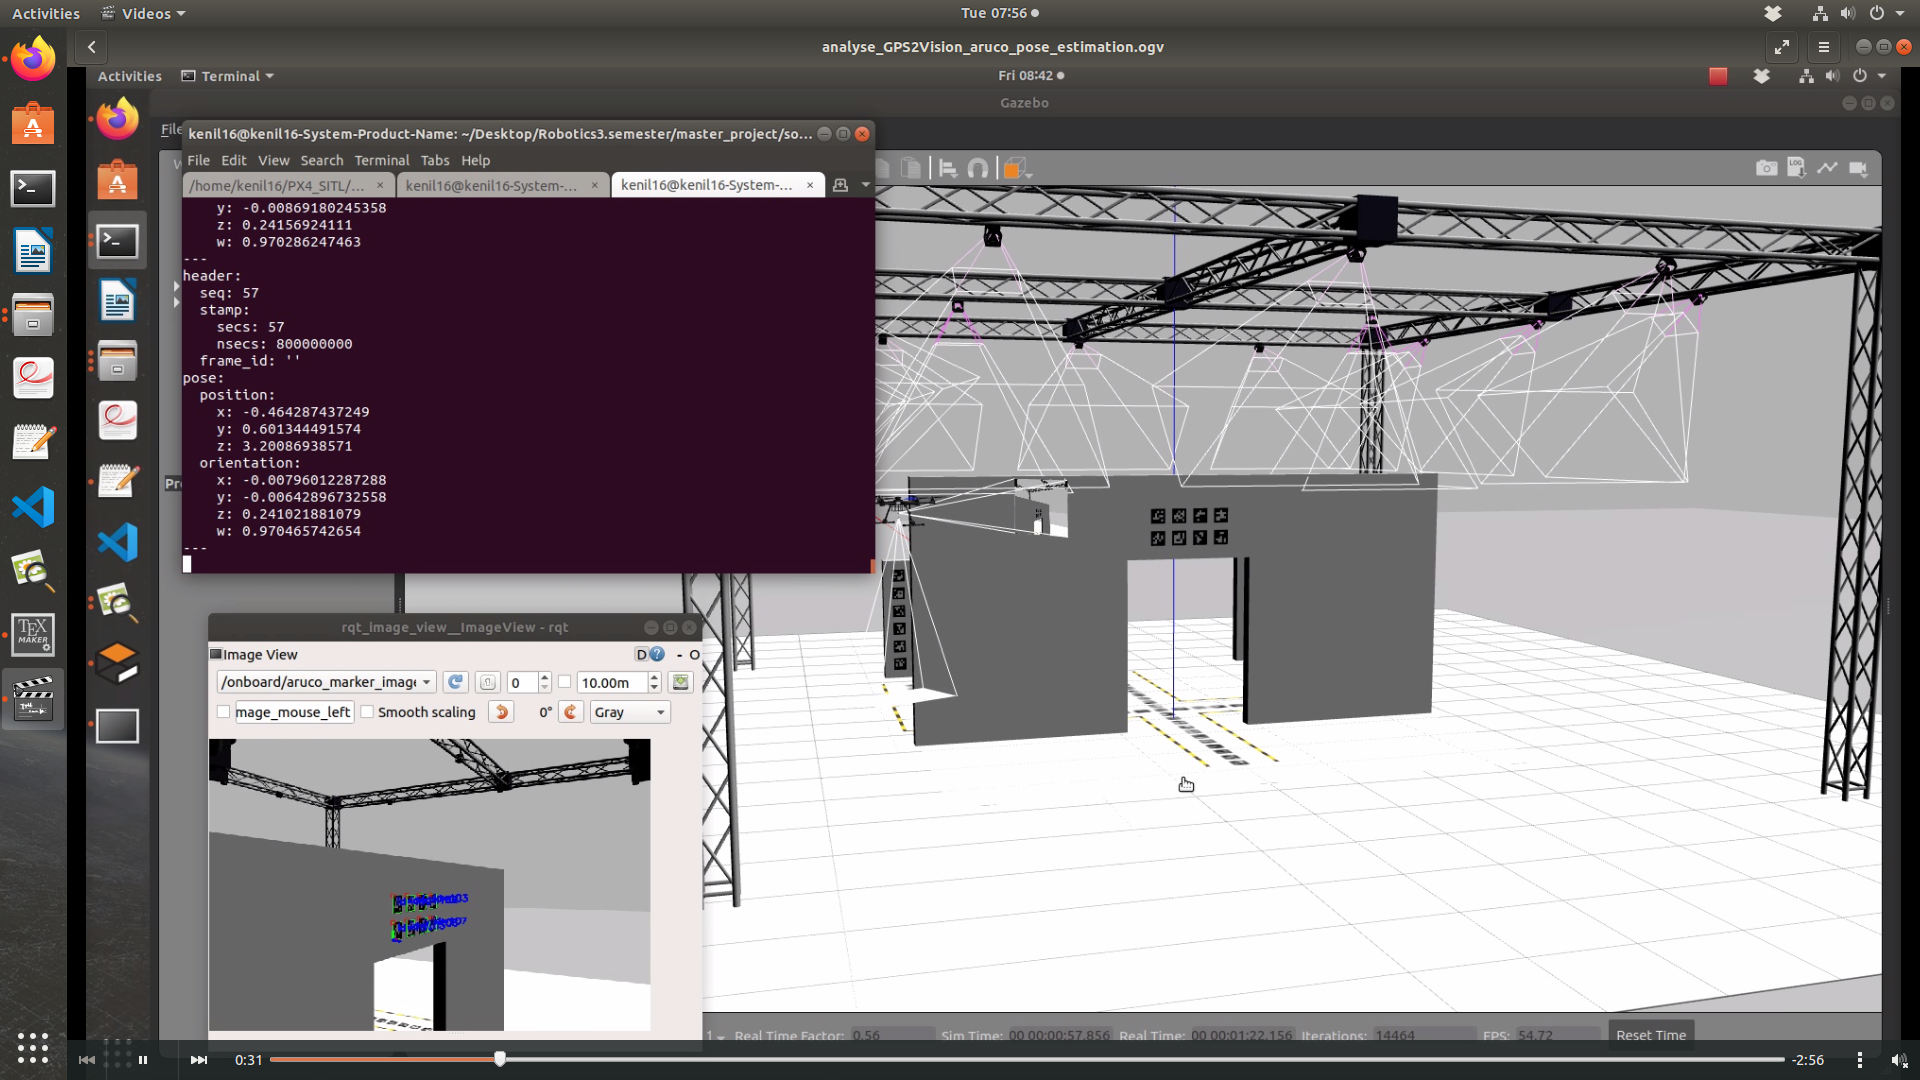
\includegraphics[width=\textwidth]{../Figures/GPS2Vision_pose_estimation_test/gps2vision_pose_estimation_one.png}
        \caption{}
        \label{fig:GPS2Vision_pose_estimation_one}
    \end{subfigure}
    \hspace{0.2em}
    \begin{subfigure}[t]{.30\textwidth}
        \centering
        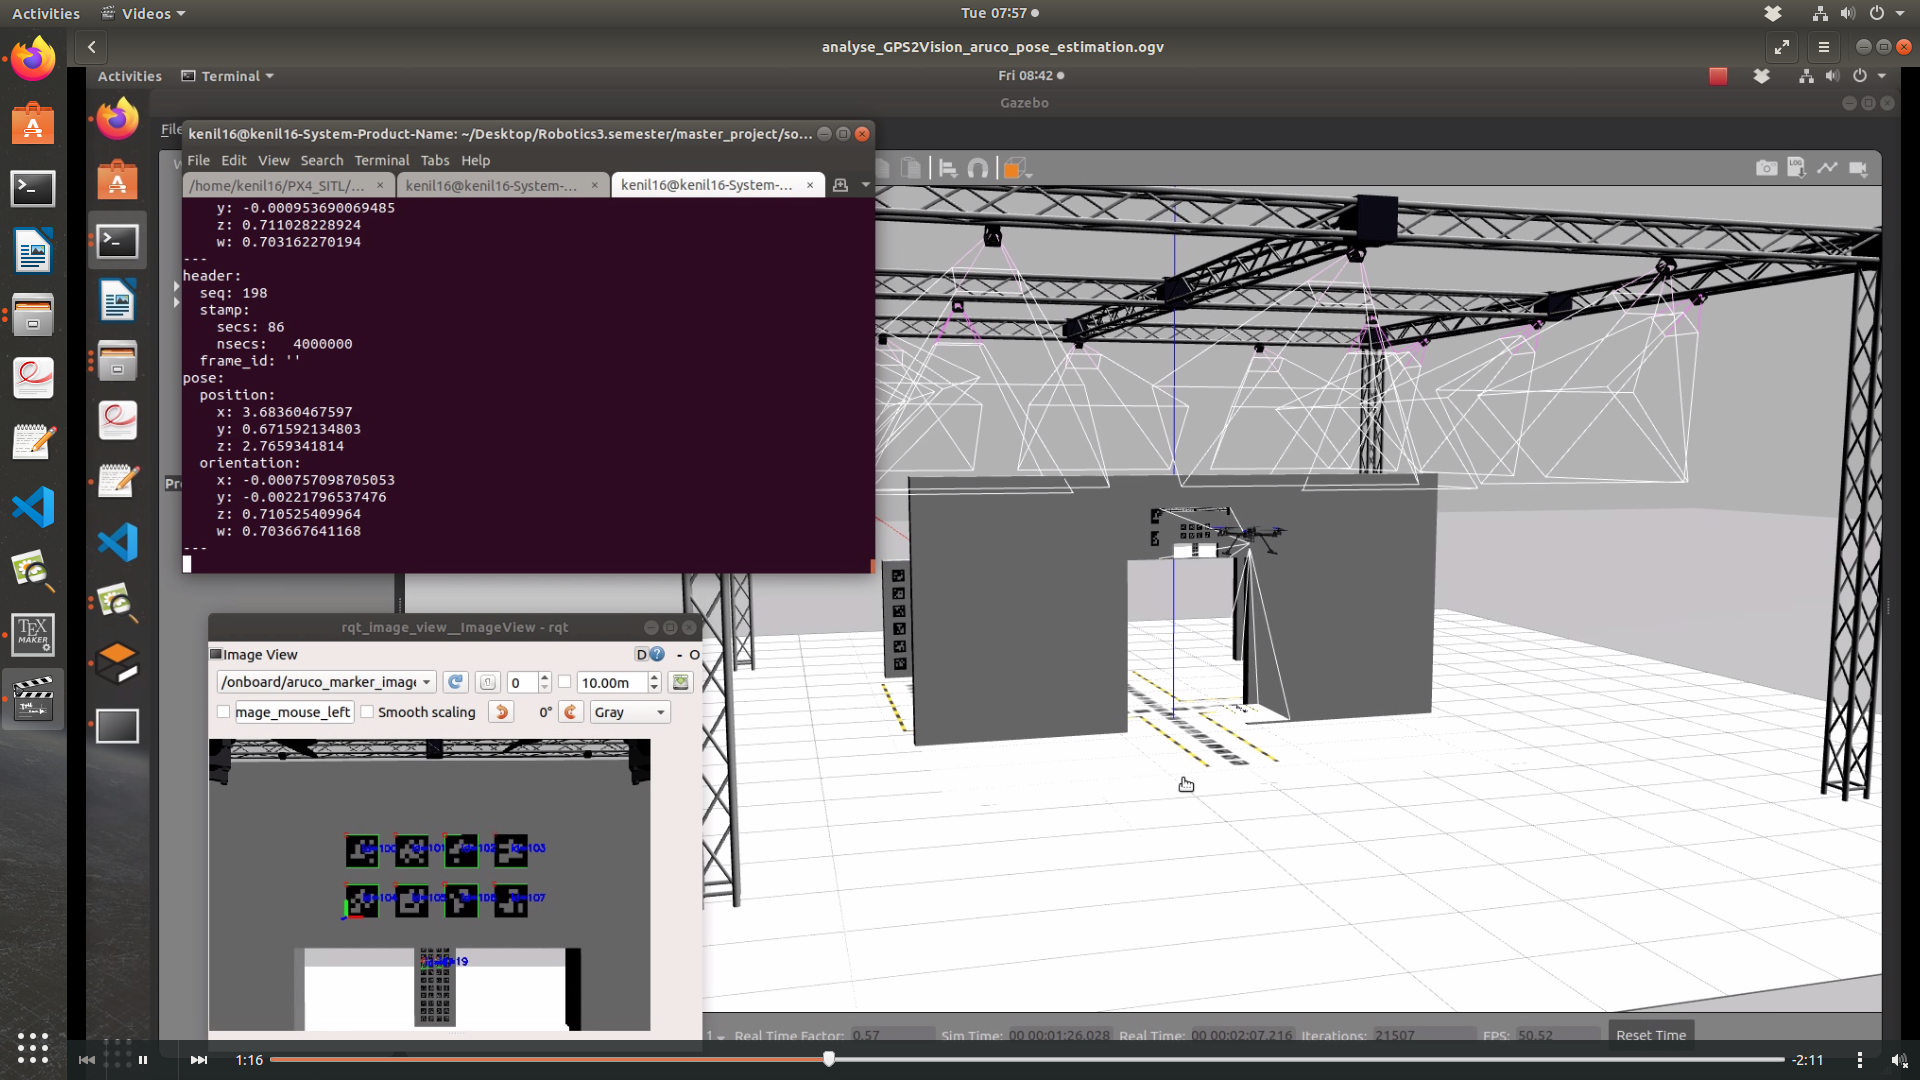
\includegraphics[width=\textwidth]{../Figures/GPS2Vision_pose_estimation_test/gps2vision_pose_estimation_two.png}
        \caption{}
        \label{fig:GPS2Vision_pose_estimation_two}
    \end{subfigure}
        \hspace{0.2em}
    \begin{subfigure}[t]{.30\textwidth}
        \centering
        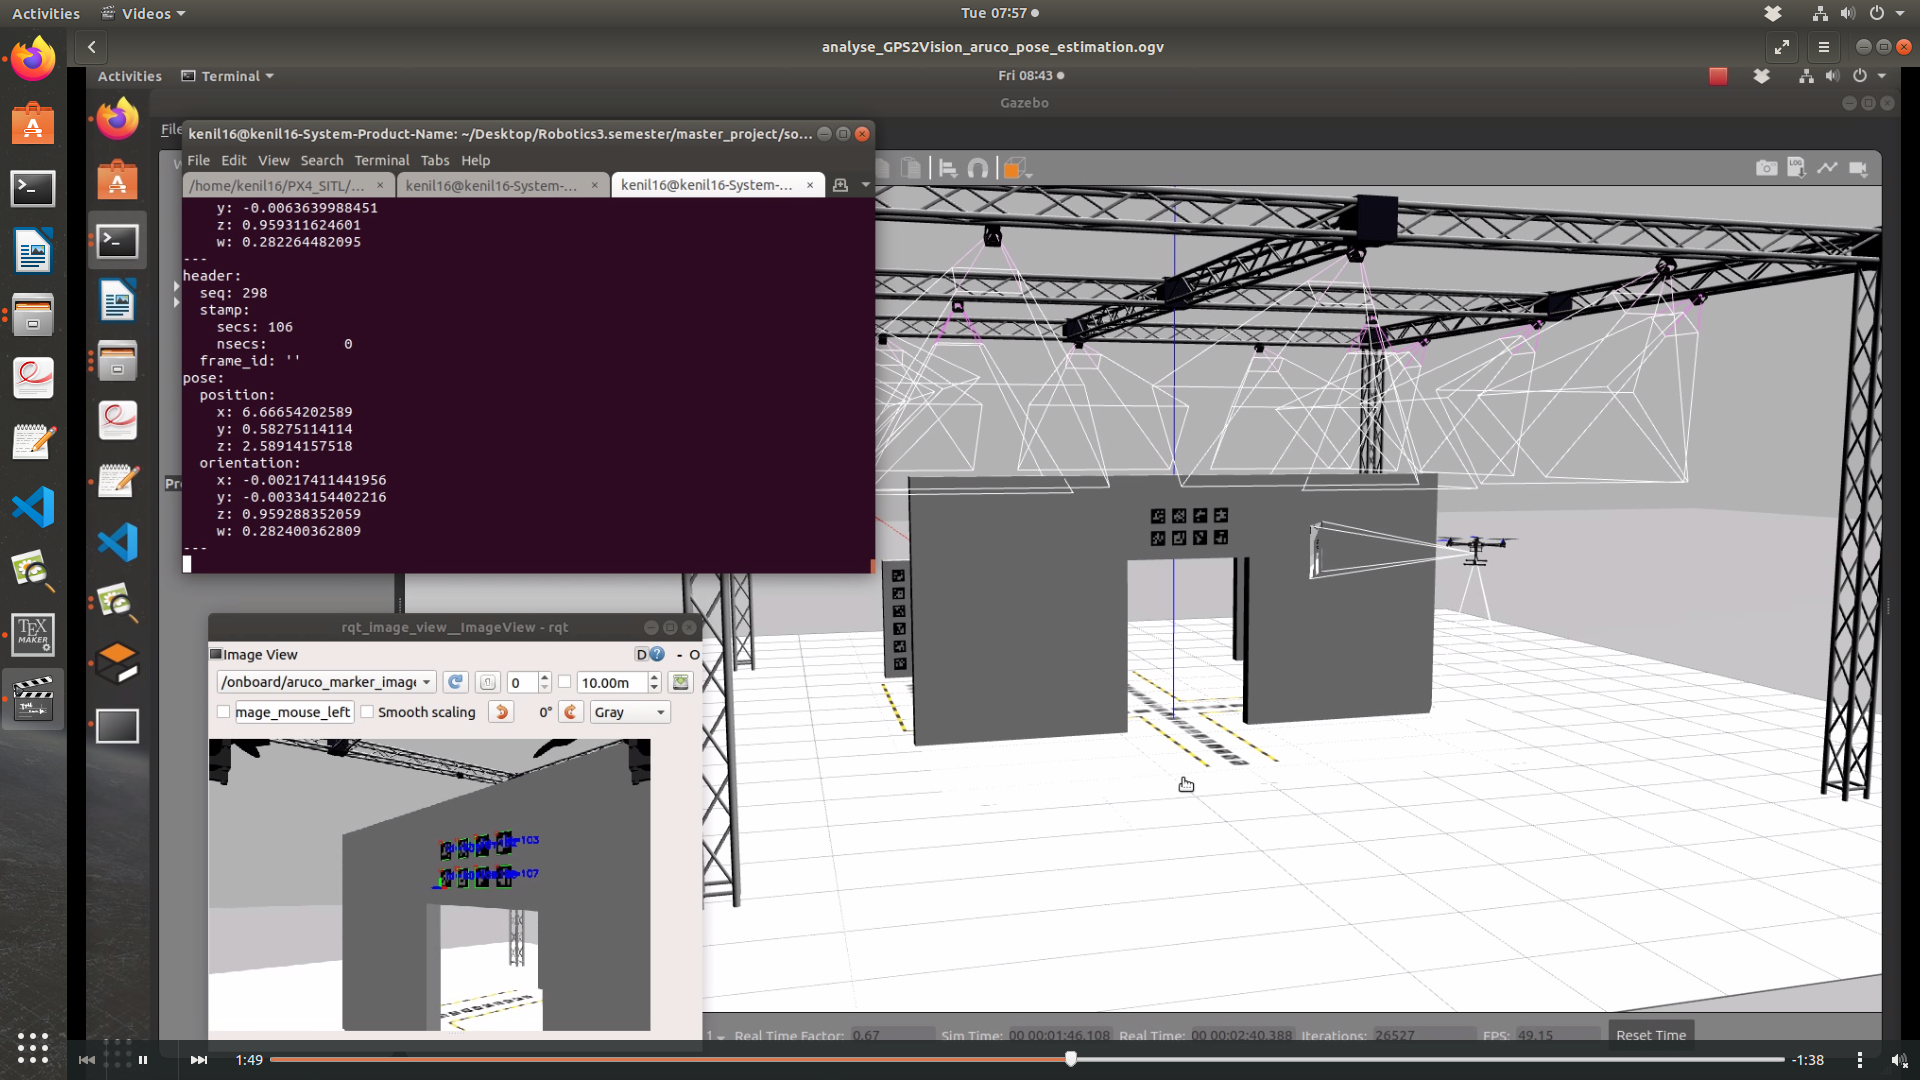
\includegraphics[width=\textwidth]{../Figures/GPS2Vision_pose_estimation_test/gps2vision_pose_estimation_three.png}
        \caption{}
        \label{fig:GPS2Vision_pose_estimation_three}
    \end{subfigure}
    \caption{Illustrations of the GPS2Vision pose estimation test in three different positions with the UAV is facing the GPS2Vision board. A video of the first couple of iterations can be seen on GitHub using \href{https://github.com/Kenil16/master_project/tree/master/test_videos/analyse_GPS2Vision_aruco_pose_estimation}{GPS2Vision pose estimation}
 }
    \label{fig:GPS2Vision_pose_estimation}
\end{figure}

\begin{figure}[H]
    \centering
    \begin{subfigure}[t]{.337\textwidth}
        \centering
        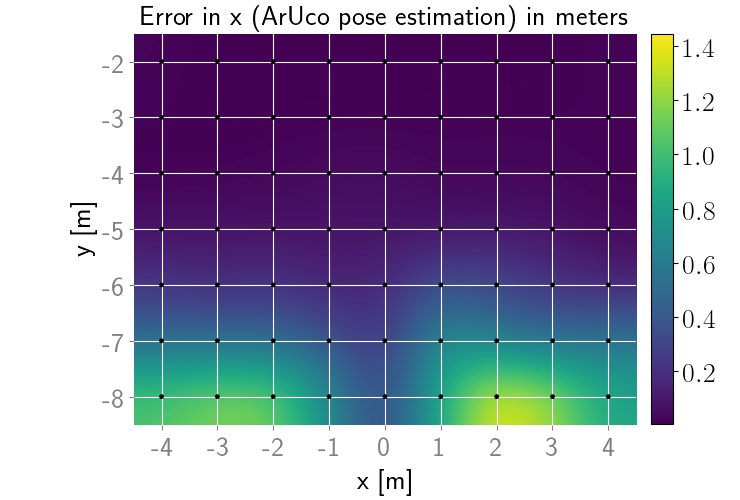
\includegraphics[width=\textwidth]{../Figures/GPS2Vision_pose_estimation_test/test1_aruco_board_width_0.2_space_0.1/aruco_pose_estimation_error_x.png}
        \caption{}
        \label{fig:GPS2Vision_pose_estimation_test1_error_x}
    \end{subfigure}
    \hspace{-0.9em}
    \begin{subfigure}[t]{.337\textwidth}
        \centering
        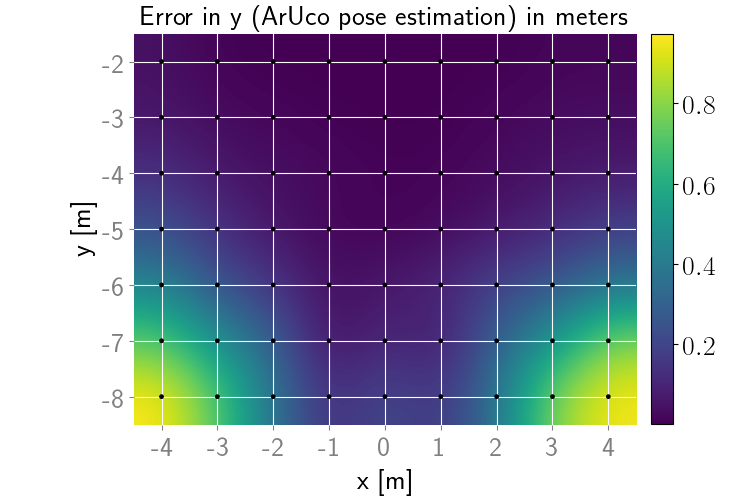
\includegraphics[width=\textwidth]{../Figures/GPS2Vision_pose_estimation_test/test1_aruco_board_width_0.2_space_0.1/aruco_pose_estimation_error_y.png}
        \caption{}
        \label{fig:GPS2Vision_pose_estimation_test1_error_y}
    \end{subfigure}
    \hspace{-0.9em}
    \begin{subfigure}[t]{.337\textwidth}
        \centering
        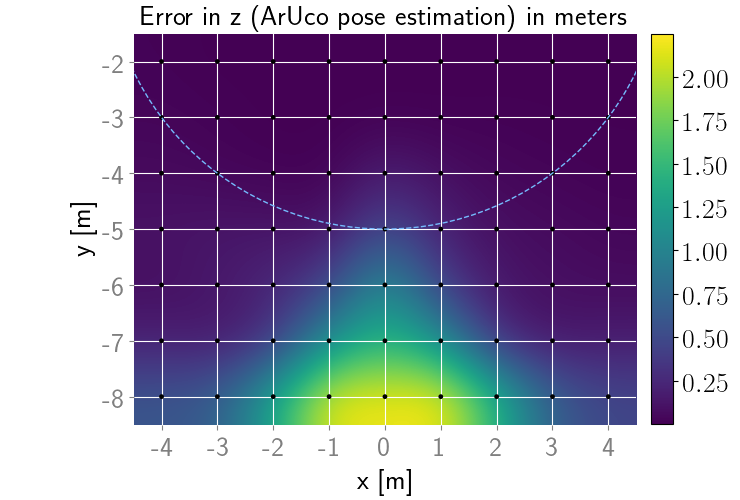
\includegraphics[width=\textwidth]{../Figures/GPS2Vision_pose_estimation_test/test1_aruco_board_width_0.2_space_0.1/aruco_pose_estimation_error_z.png}
        \caption{}
        \label{fig:GPS2Vision_pose_estimation_test1_error_z}
    \end{subfigure}
    \caption{Black dots indicates where the UAV has estimated the pose of the ArUco board and the circle colored sky blue indicates a safe GPS2Vision transition area. It may the noticed that the error in the position estimate becomes quite high when the UAV has a distance of 7-8 meters away from the GPS2Vision board}
    \label{fig:GPS2Vision_pose_estimation_test1_error_pos}
\end{figure}

\begin{figure}[H]
    \centering
    \begin{subfigure}[t]{.337\textwidth}
        \centering
        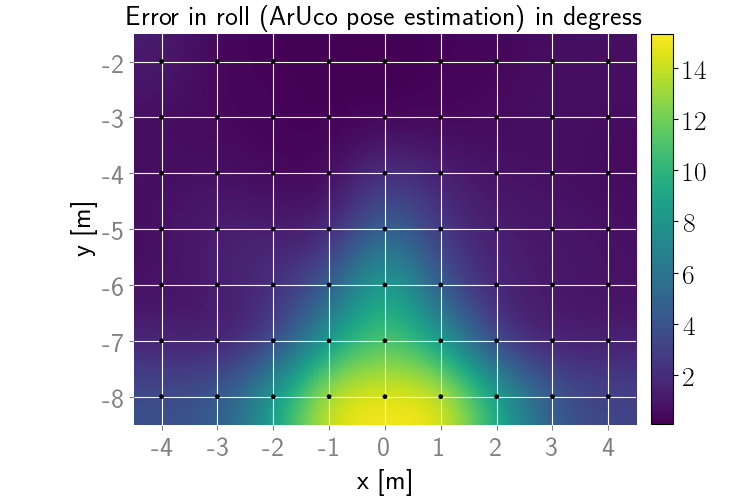
\includegraphics[width=\textwidth]{../Figures/GPS2Vision_pose_estimation_test/test1_aruco_board_width_0.2_space_0.1/aruco_pose_estimation_error_roll.png}
        \caption{}
        \label{fig:GPS2Vision_pose_estimation_test1_error_roll}
    \end{subfigure}
    \hspace{-0.9em}
    \begin{subfigure}[t]{.337\textwidth}
        \centering
        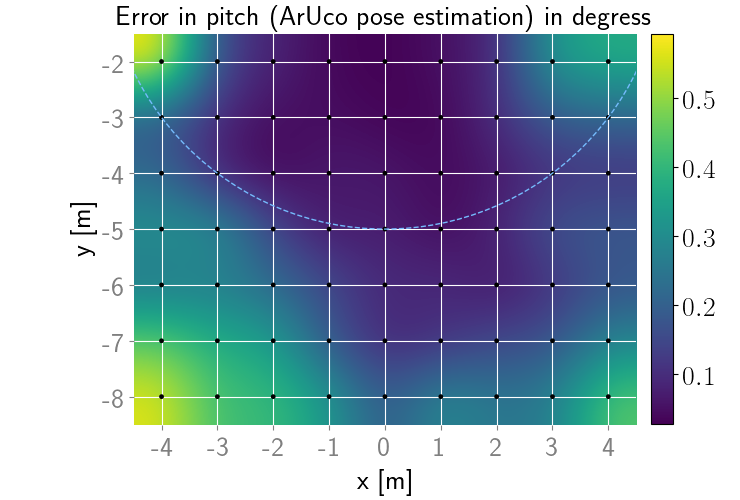
\includegraphics[width=\textwidth]{../Figures/GPS2Vision_pose_estimation_test/test1_aruco_board_width_0.2_space_0.1/aruco_pose_estimation_error_pitch.png}
        \caption{}
        \label{fig:GPS2Vision_pose_estimation_test1_error_pitch}
    \end{subfigure}
    \hspace{-0.9em}
    \begin{subfigure}[t]{.337\textwidth}
        \centering
        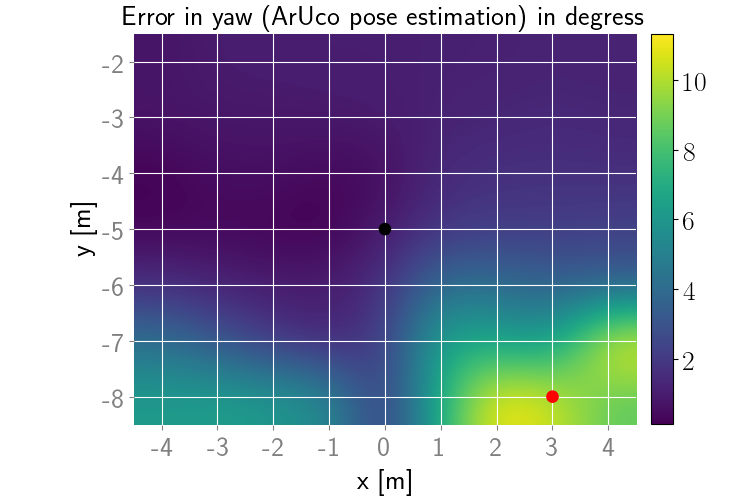
\includegraphics[width=\textwidth]{../Figures/GPS2Vision_pose_estimation_test/test1_aruco_board_width_0.2_space_0.1/aruco_pose_estimation_error_yaw.png}
        \caption{}
        \label{fig:GPS2Vision_pose_estimation_test1_error_yaw}
    \end{subfigure}
    \caption{Black dots indicates where the UAV has estimated the pose of the ArUco board and the circle colored sky blue indicates a safe GPS2Vision transition area. It may the noticed that the error in the angle estimate becomes quite high when the UAV has a distance of 7-8 meters away from the GPS2Vision board}
    \label{fig:GPS2Vision_pose_estimation_test1_error_ori}
\end{figure}

In order to replicate the test, the command in Listing \ref{lst:GPS2Vision_pose_estimation_test} can be run from the terminal.

\definecolor{lightgreen}{rgb}{0.56, 0.93, 0.56}
\definecolor{moonstoneblue}{rgb}{0.45, 0.66, 0.76}
\begin{listing}[H] 
\begin{tcolorbox}[
    enhanced,
    attach boxed title to top left={xshift=6mm,yshift=-3mm},
    colback=lightgreen!20,
    colframe=lightgreen,
    fonttitle=\bfseries\color{black},
]
\begin{minted}[ numbersep=6pt, linenos=true, breaklines=true, breakanywhere=true, mathescape, escapeinside=||,fontsize=\small]{bash}
#For execution of the giving test
roslaunch px4 gazebo_sim_v1.0.launch worlds:=optitrack_big_board_onepattern.world drone_control_args:="GPS2Vision_aruco_pose_estimation_test" x:=-3.0 y:=0.0 headless:=false gui:=true
\end{minted}
\end{tcolorbox}
\caption{Command to be used to replicate the test}
\label{lst:GPS2Vision_pose_estimation_test}    
\end{listing} 

\subsubsection{Rolling average from ArUco pose estimation}
\label{sec:rolling_average_aruco_pose_estimation}

\begin{figure}[H]
    \centering
    \begin{subfigure}[t]{.30\textwidth}
        \centering
        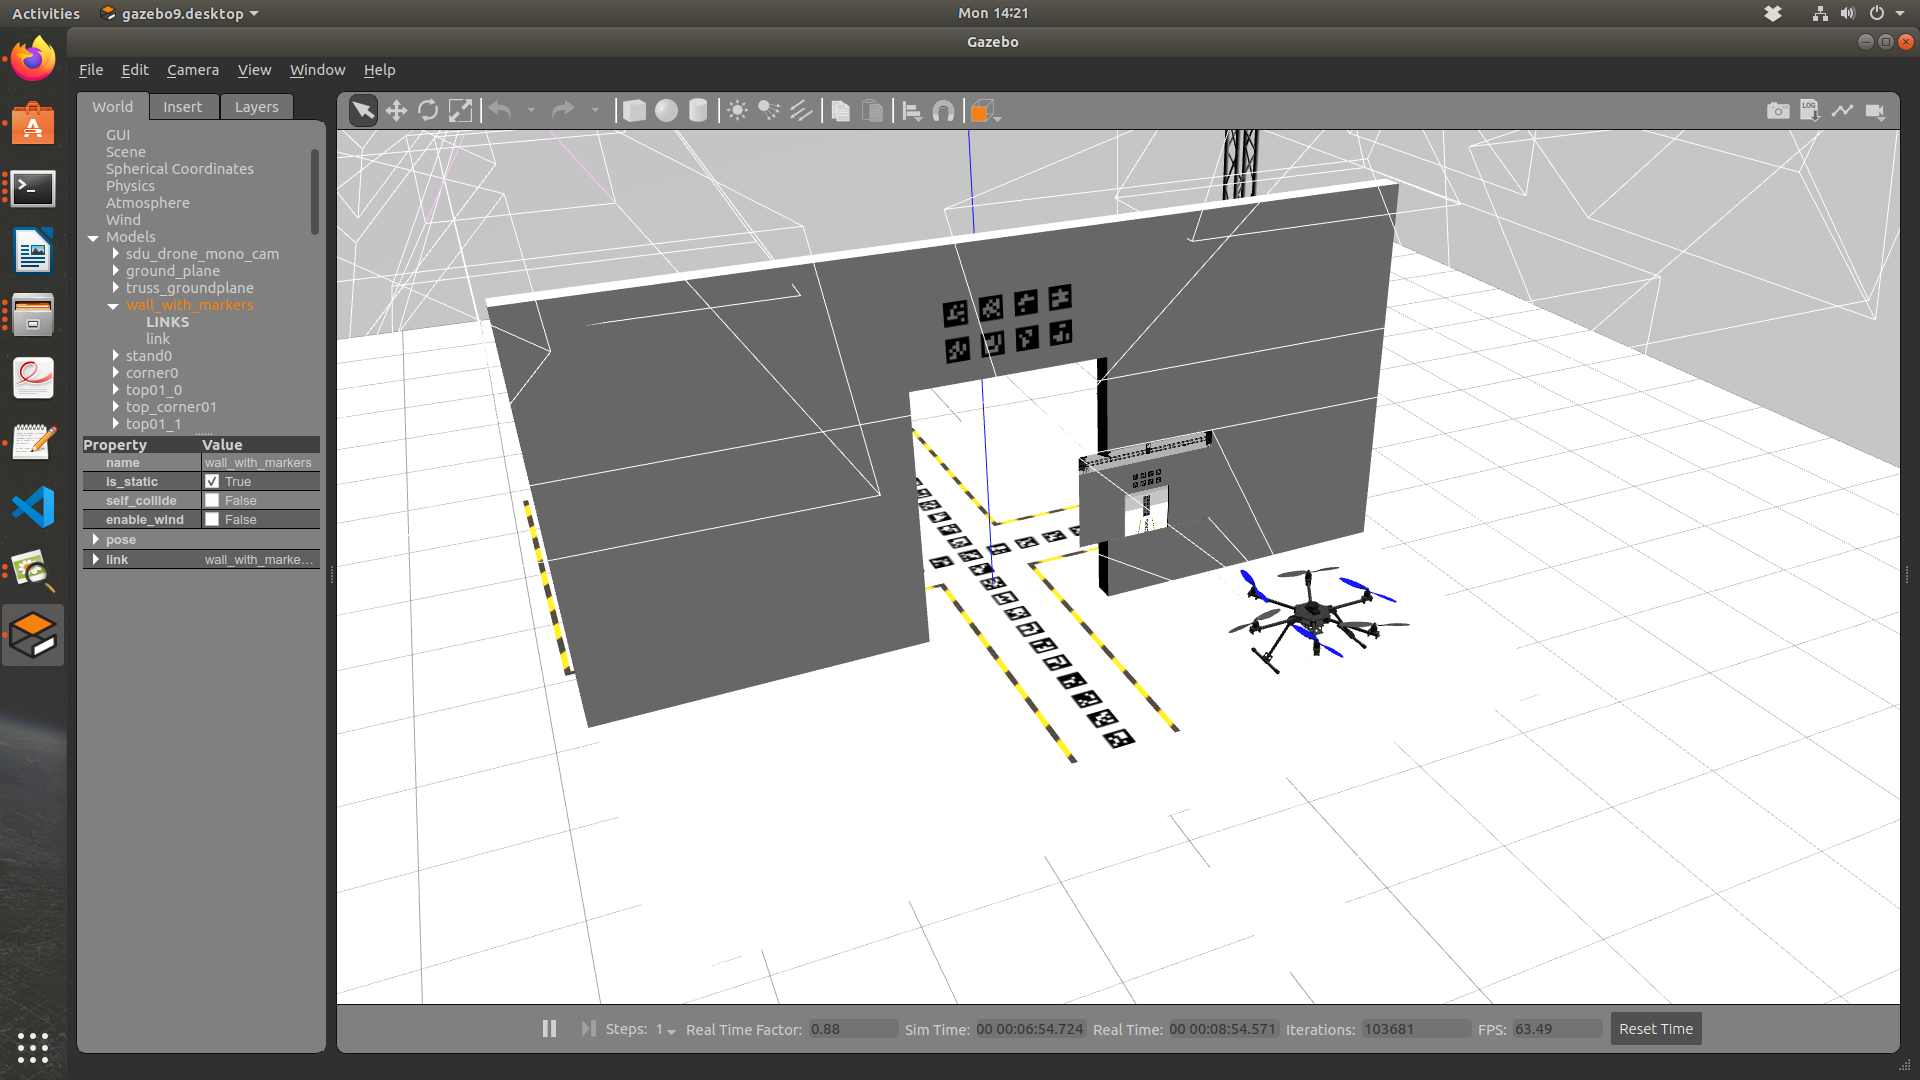
\includegraphics[width=\textwidth]{../Figures/analyse_rolling_average/optimal_pose.png}
        \caption{}
        \label{fig:rolling_average_good_pos}
    \end{subfigure}
    \hspace{0.5em}
    \begin{subfigure}[t]{.30\textwidth}
        \centering
        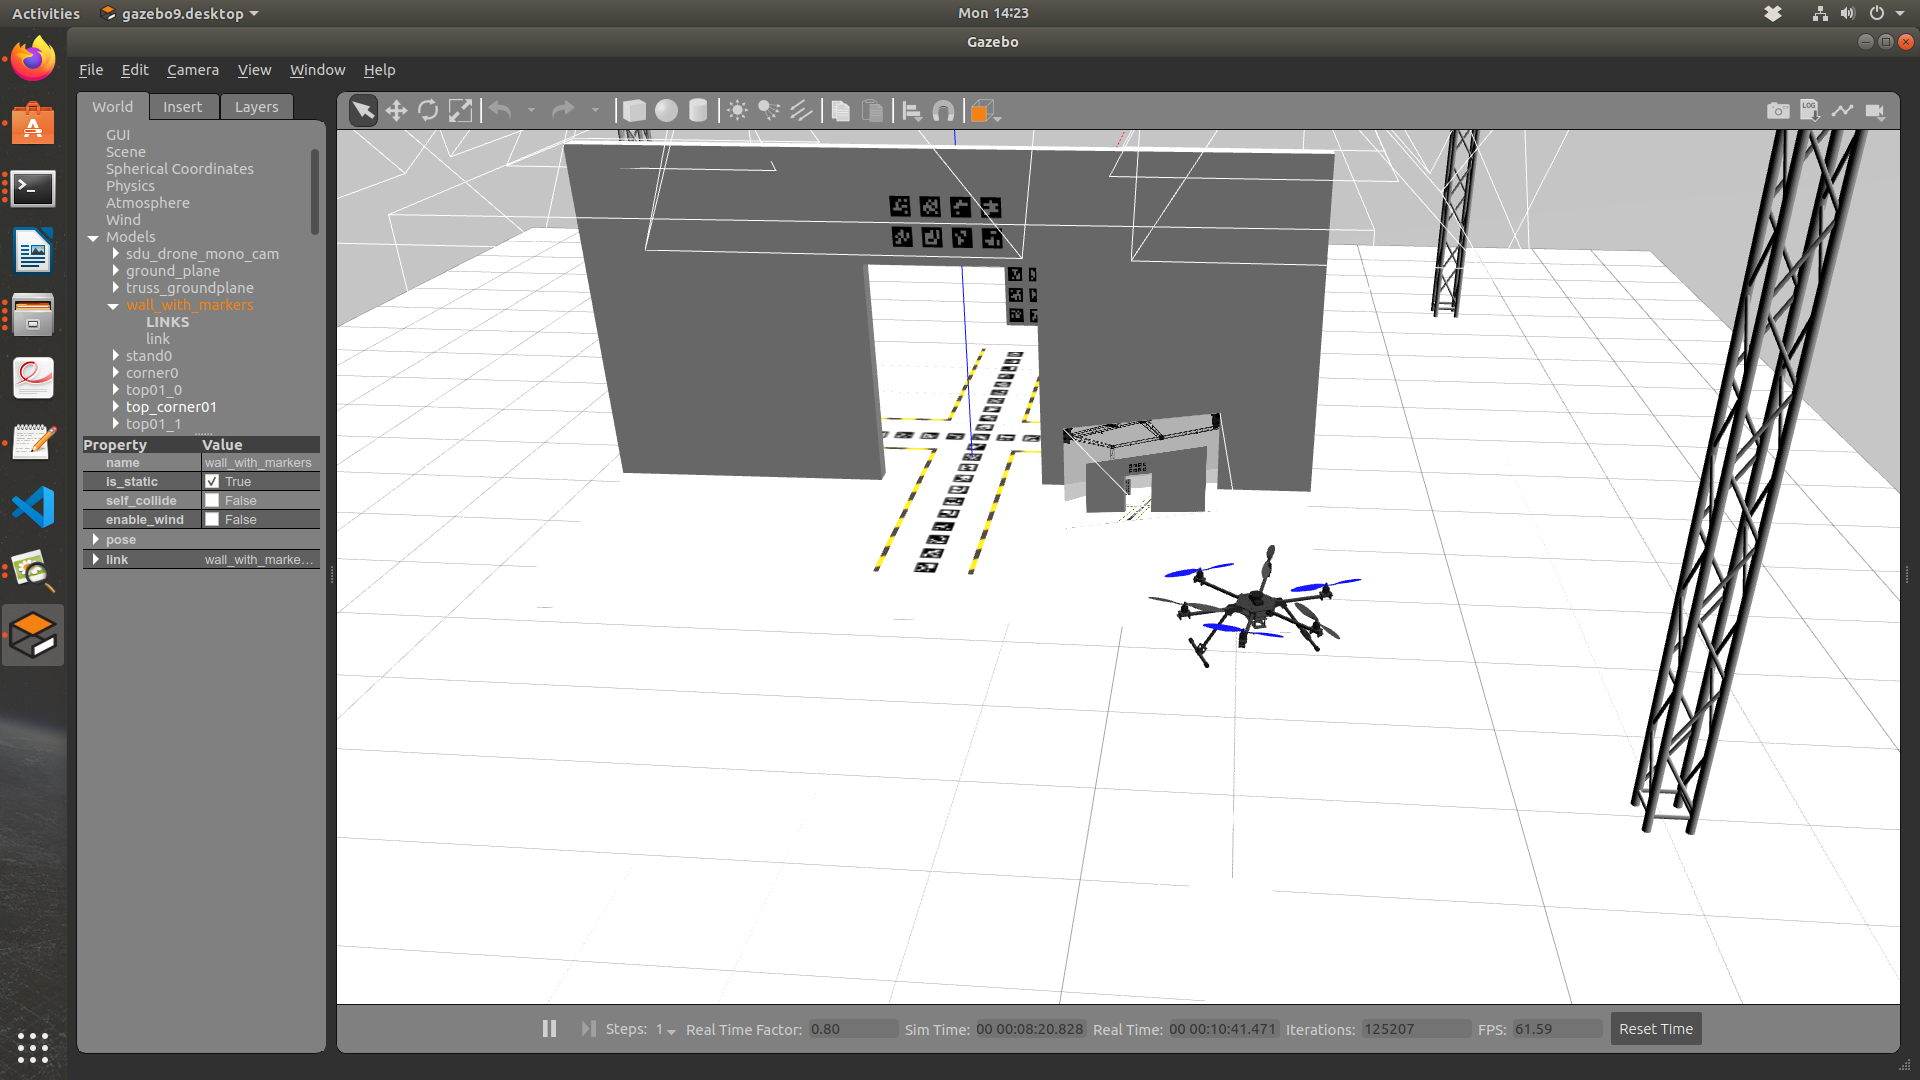
\includegraphics[width=\textwidth]{../Figures/analyse_rolling_average/bad_pose.png}
        \caption{}
        \label{fig:rolling_average_bad_pos}
    \end{subfigure}
    \caption{Illustrations of the two positions used to evaluate the rolling average for one-hundred iterations. The positions of the UAV in Figures \ref{fig:rolling_average_good_pos} and \ref{fig:rolling_average_bad_pos} are (0,-5) and (3,-7) respectively from the coordinate system in Figures \ref{fig:GPS2Vision_pose_estimation_test1_error_pos} and \ref{fig:GPS2Vision_pose_estimation_test1_error_ori}} 
    \label{fig:rolling_average_pos}
\end{figure}

To analyze the possibility of fluctuations in the ArUco pose estimates, the rolling average is used for calculating the mean and standard deviation (STD) in two different positions for one-hundred iterations. This can be seen in Figure \ref{fig:rolling_average_pos}. 

\begin{figure}[H]
    \centering
    \begin{subfigure}[t]{.30\textwidth}
        \centering
        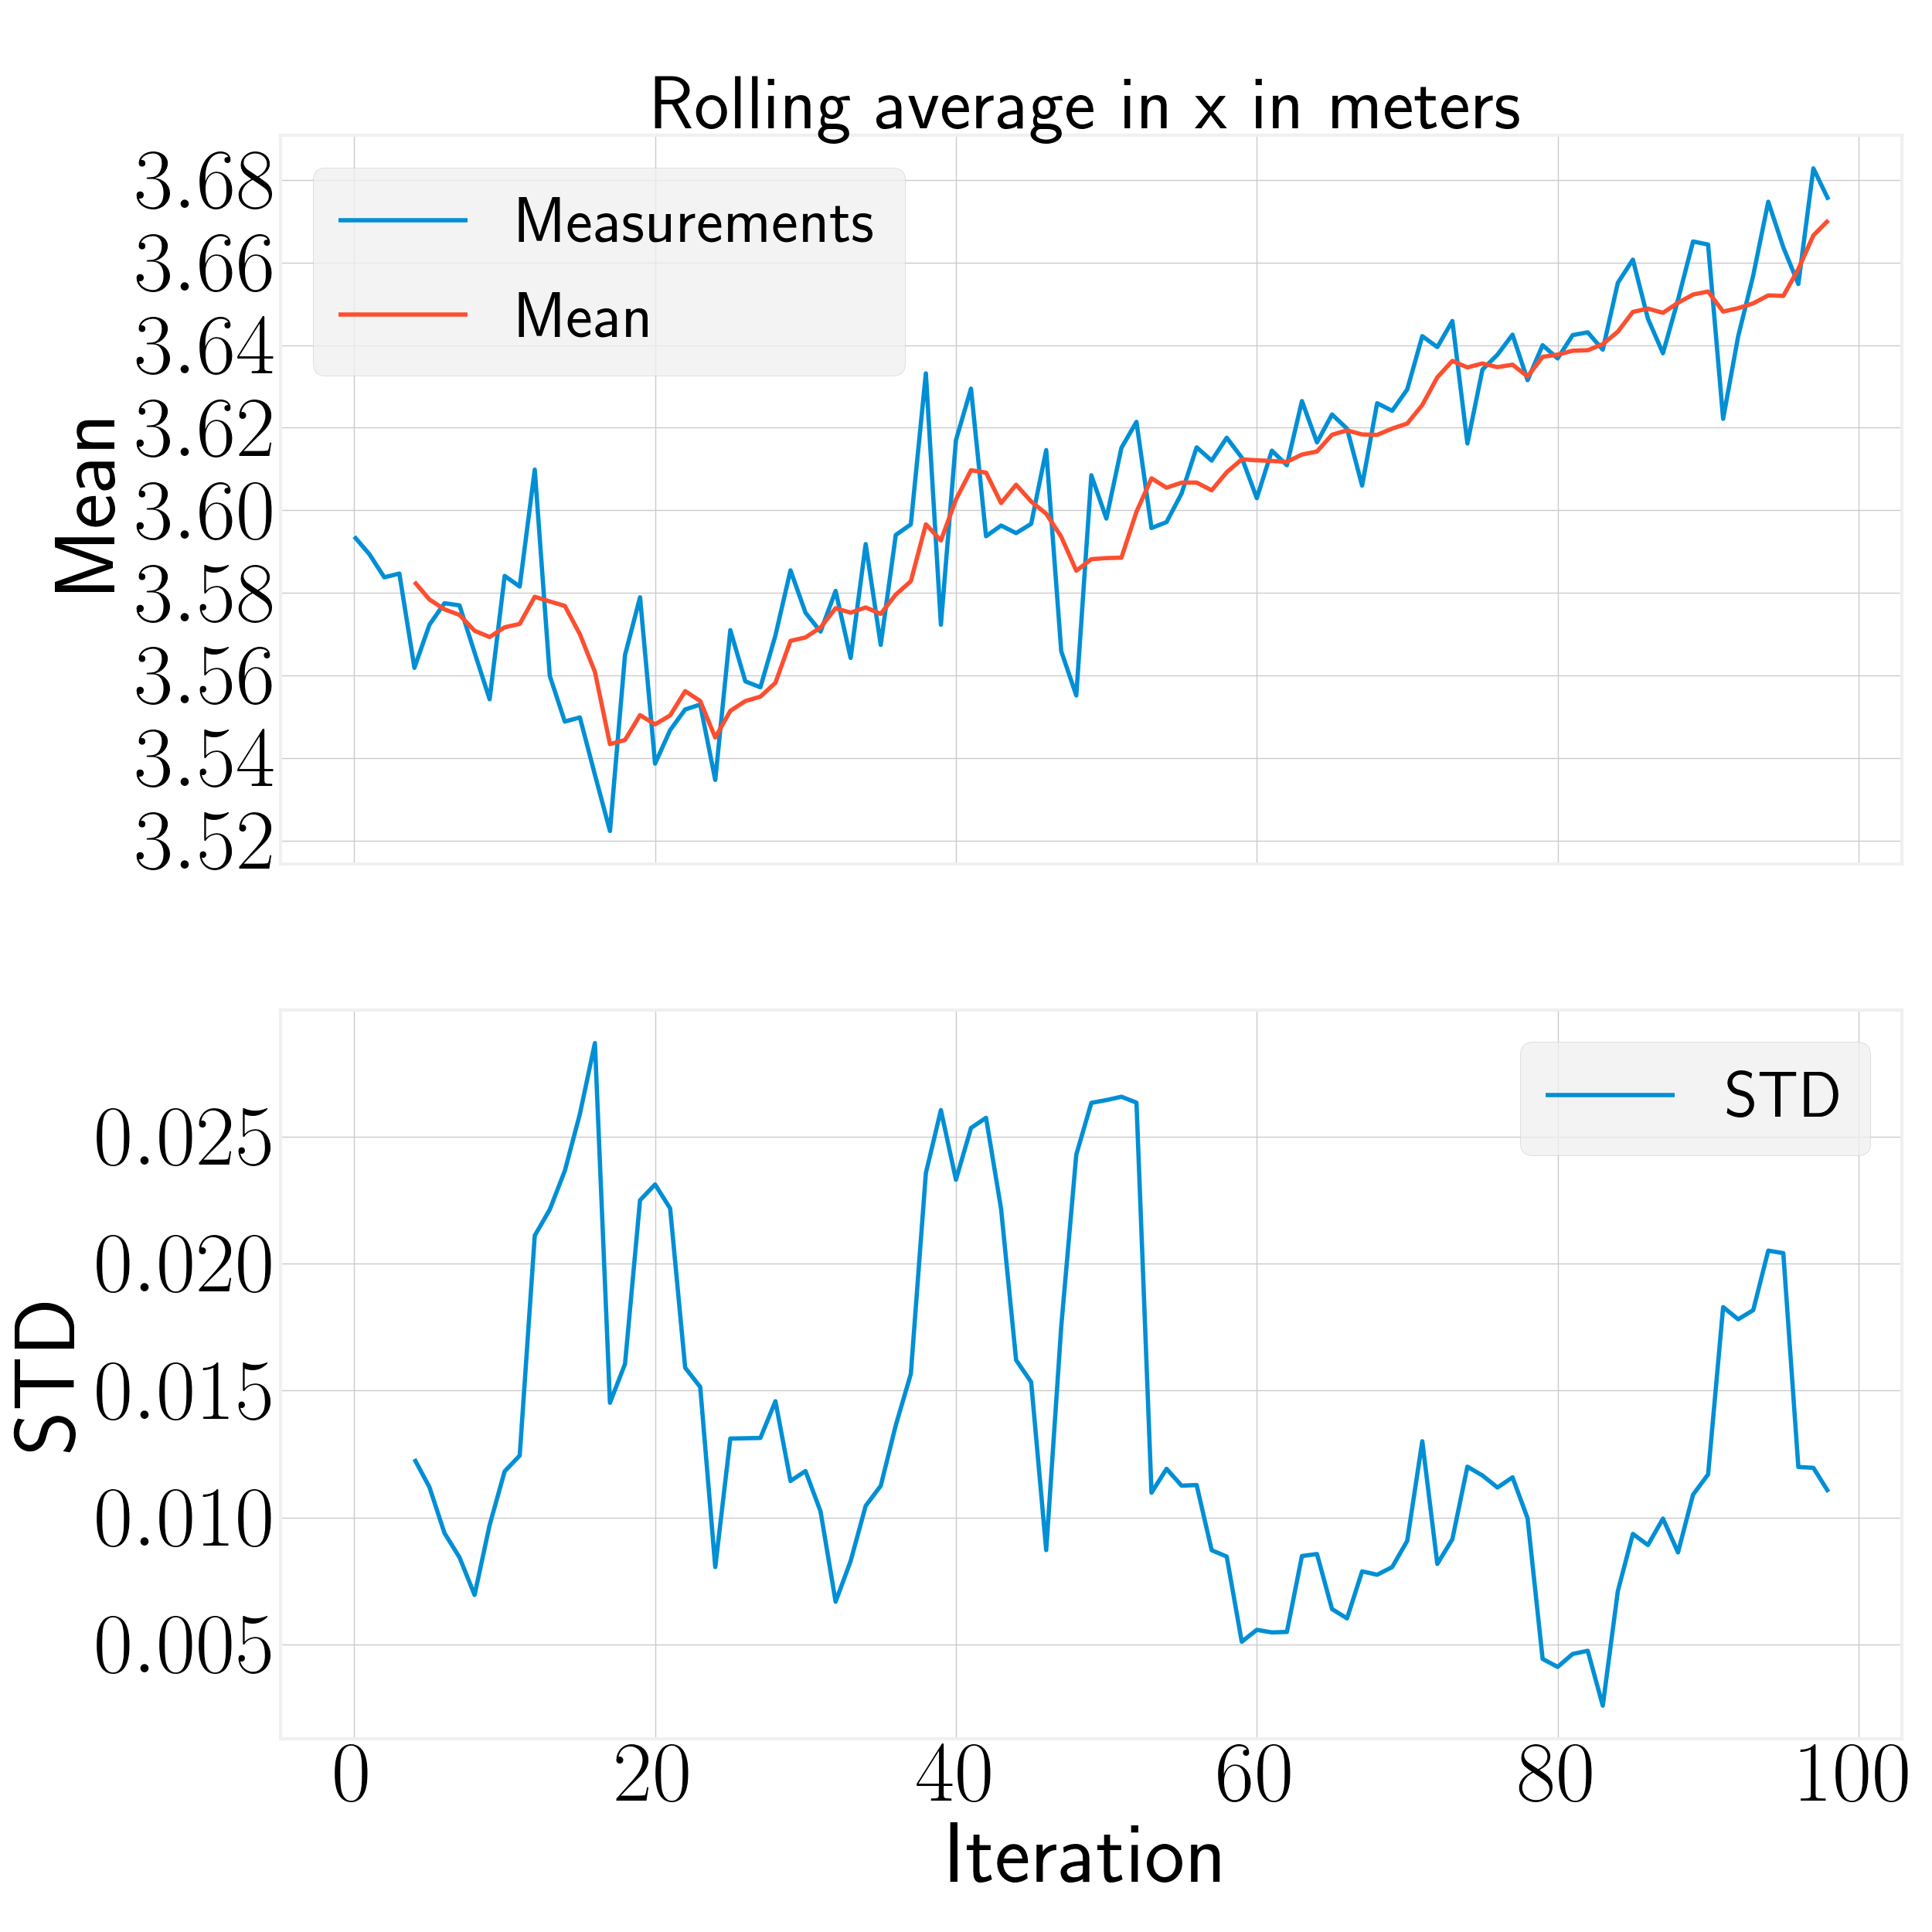
\includegraphics[width=\textwidth]{../Figures/analyse_rolling_average/test1/Calculated_rolling_average_in_x_with_mean_and_STD.png}
        \caption{}
        \label{fig:rolling_average_in_x_test1}
    \end{subfigure}
     \hspace{0.2em}
    \begin{subfigure}[t]{.30\textwidth}
        \centering
        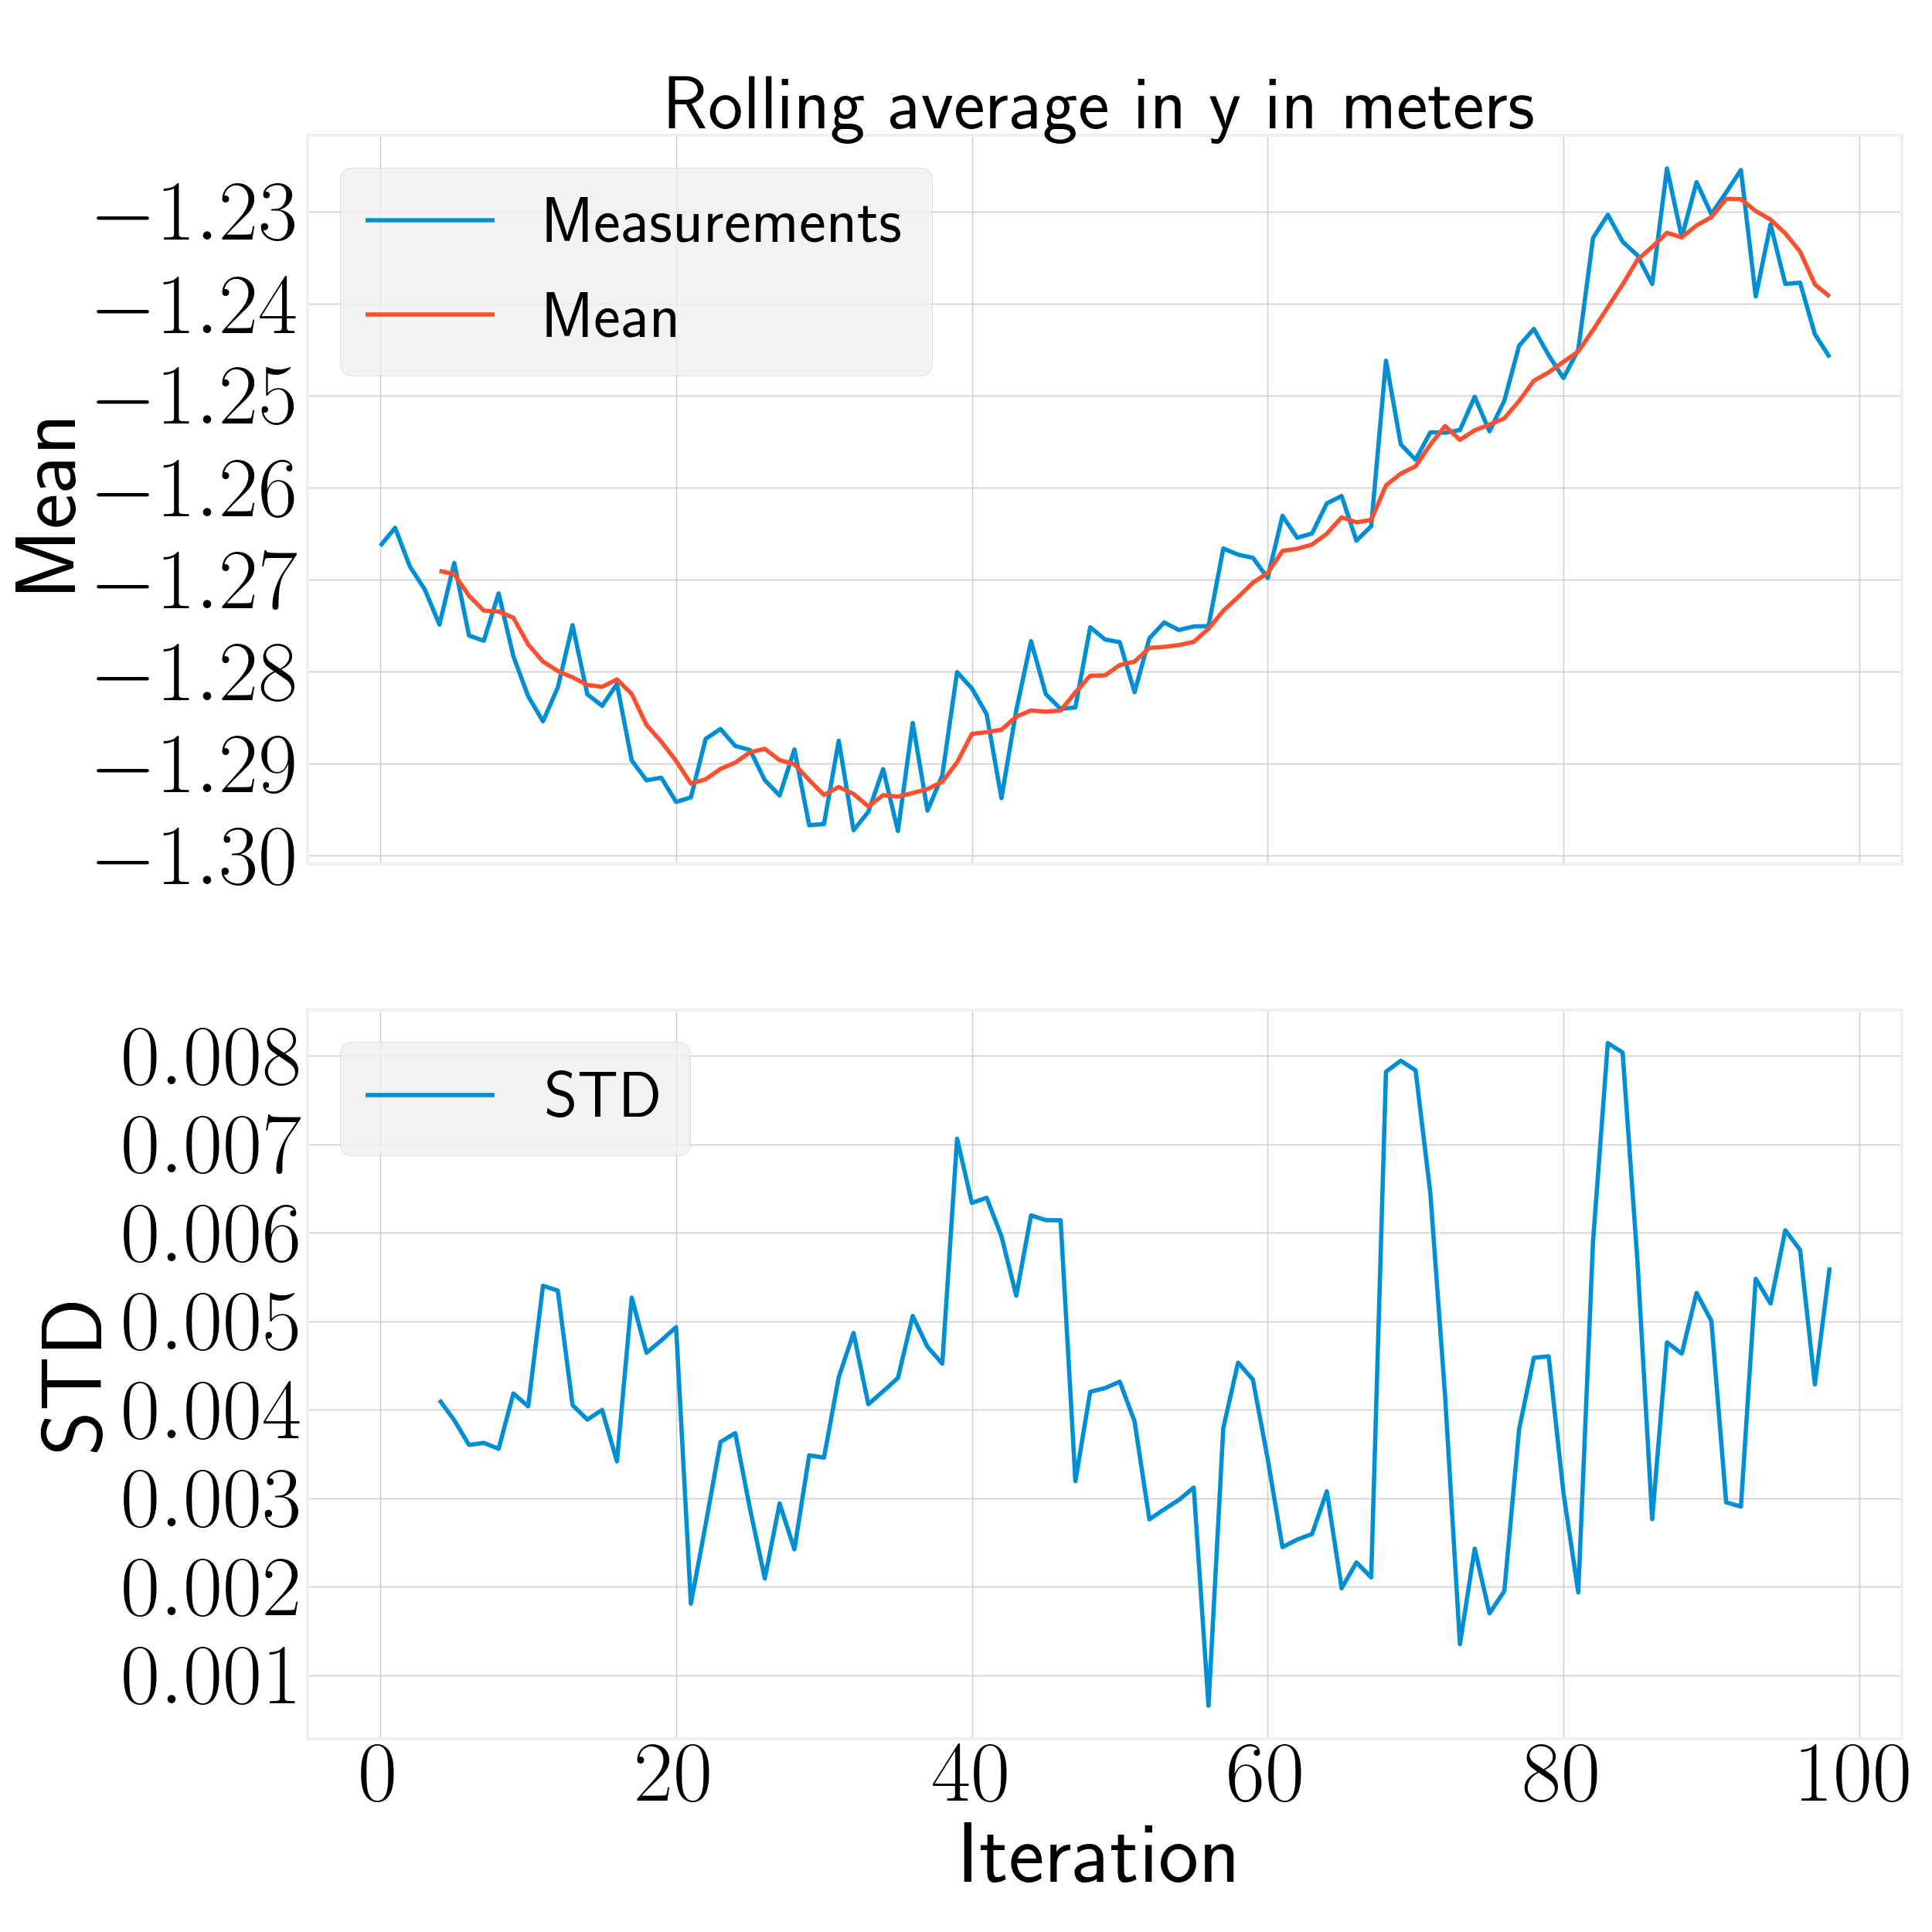
\includegraphics[width=\textwidth]{../Figures/analyse_rolling_average/test1/Calculated_rolling_average_in_y_with_mean_and_STD.png}
        \caption{}
        \label{fig:rolling_average_in_y_test1}
    \end{subfigure}
     \hspace{0.2em}
    \begin{subfigure}[t]{.30\textwidth}
        \centering
        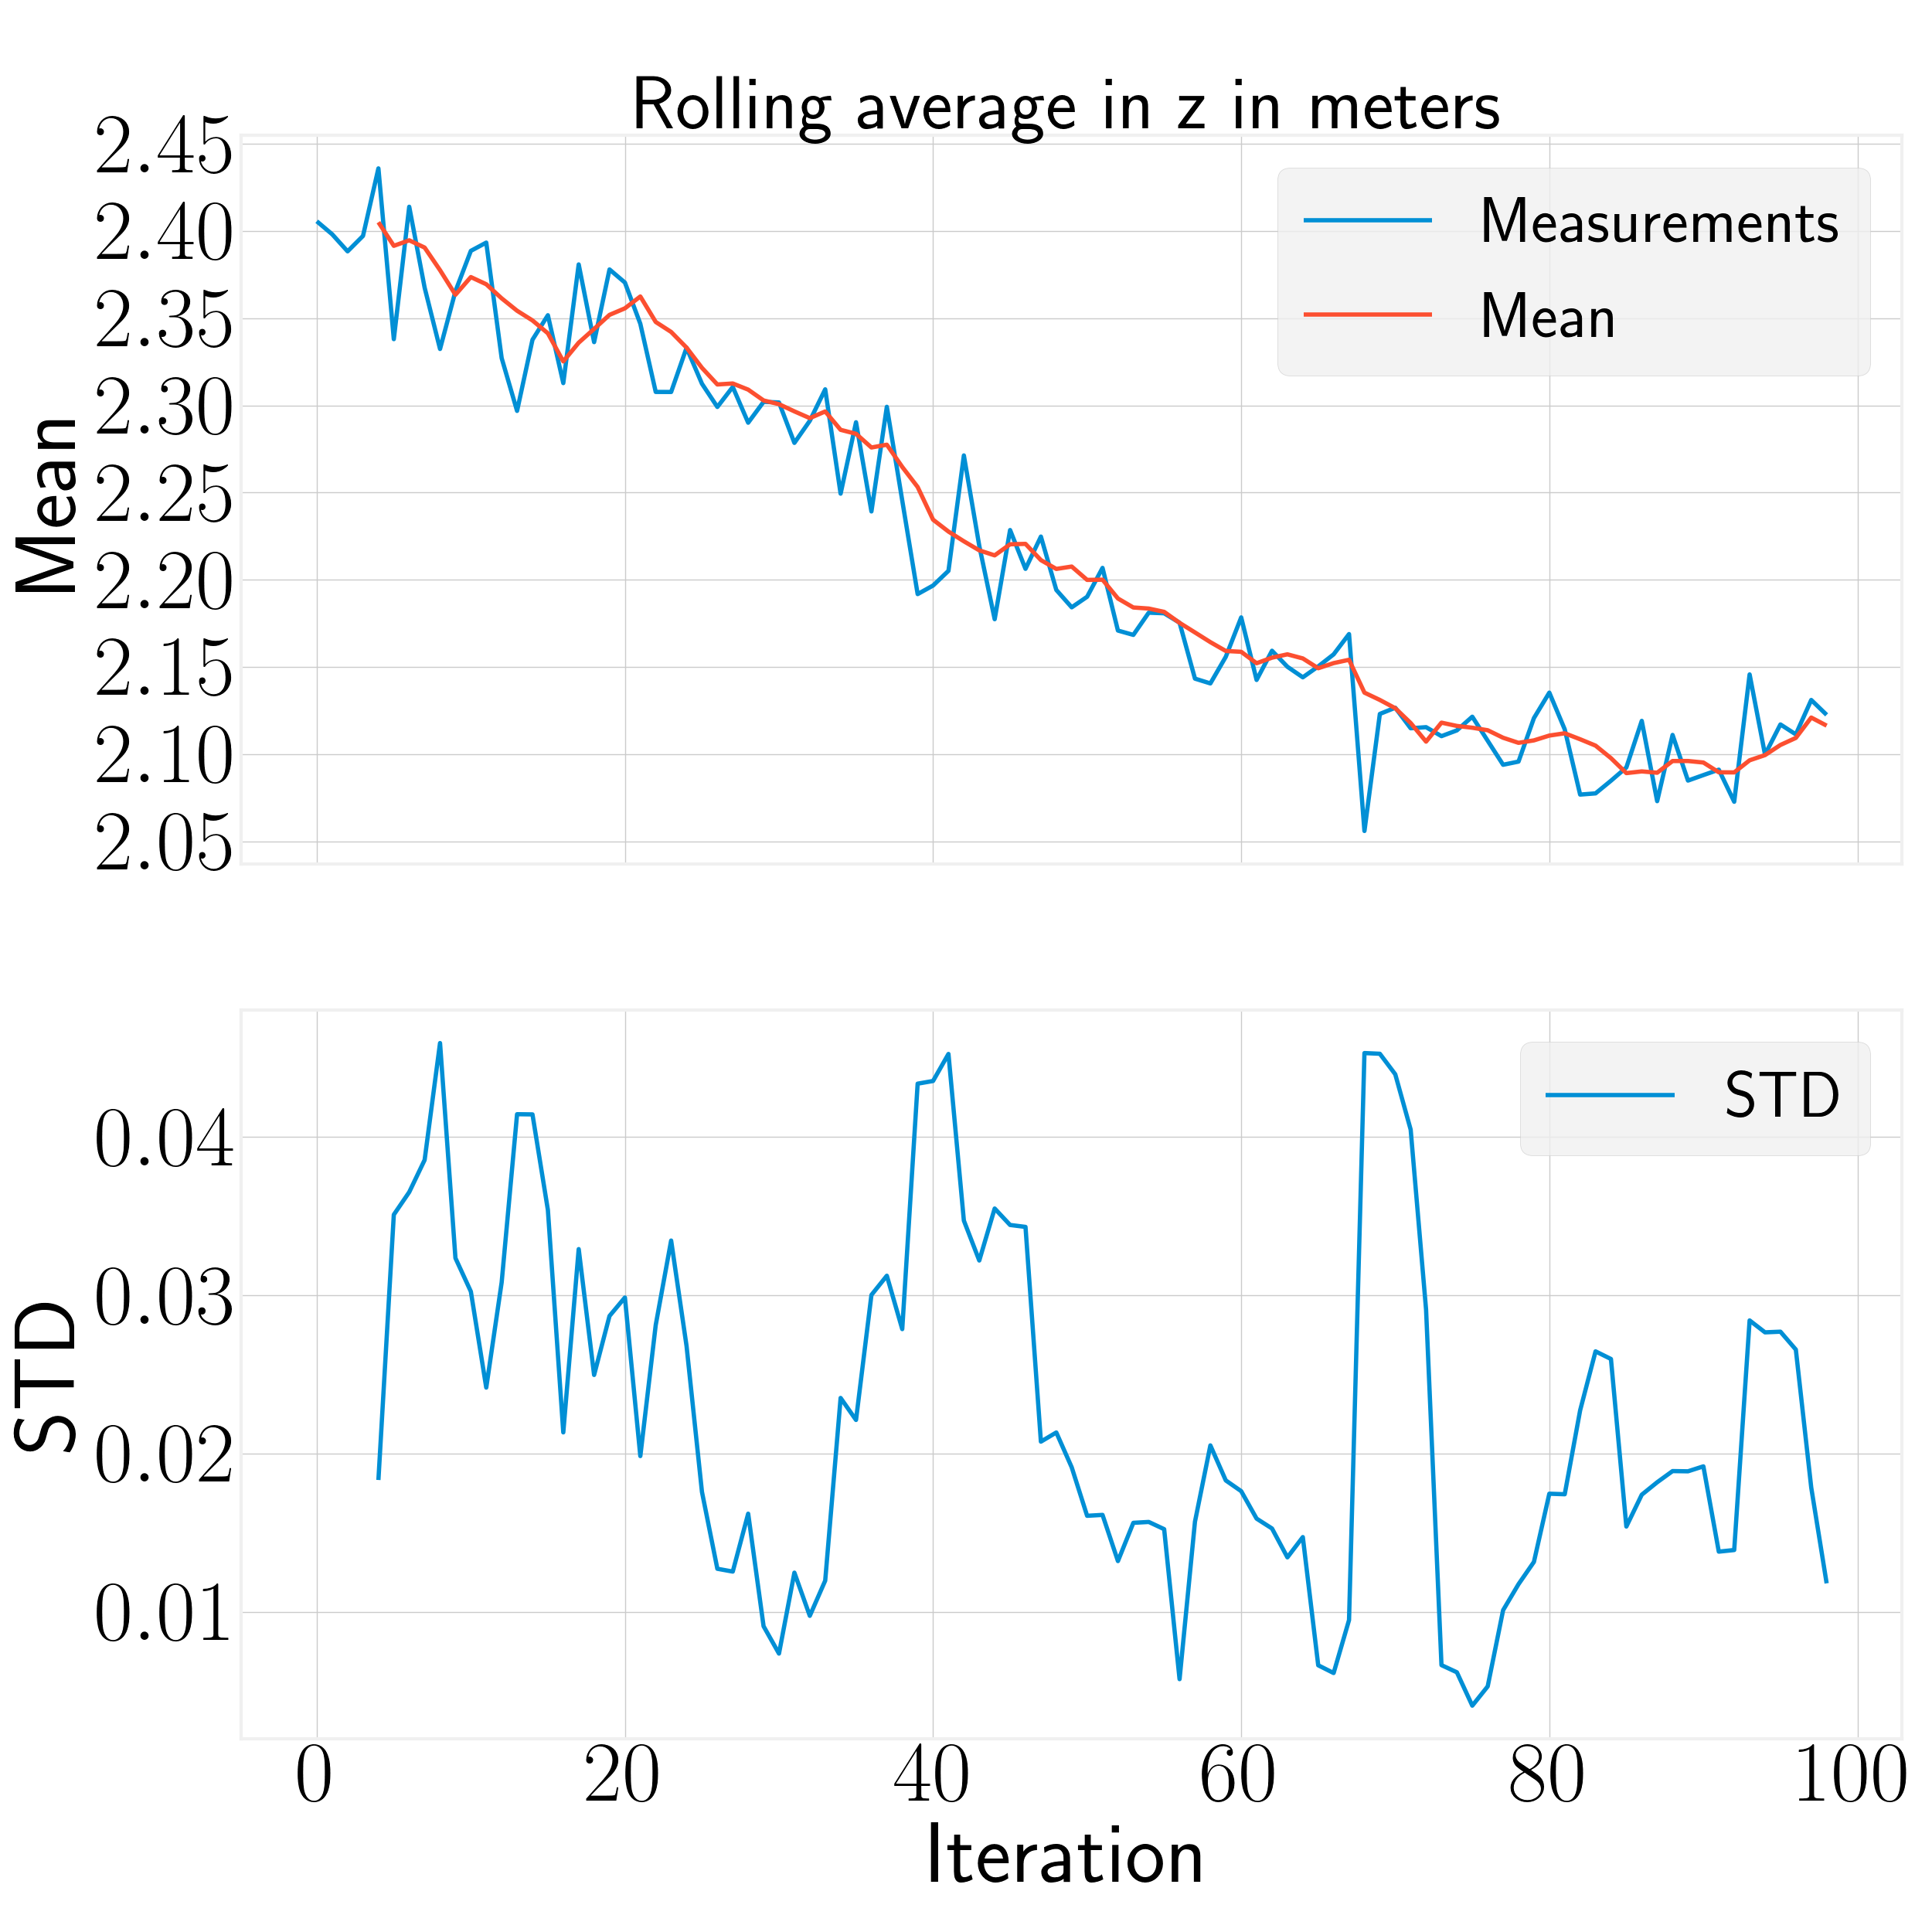
\includegraphics[width=\textwidth]{../Figures/analyse_rolling_average/test1/Calculated_rolling_average_in_z_with_mean_and_STD.png}
        \caption{}
        \label{fig:rolling_average_in_z_test1}
    \end{subfigure}
    \caption{Illustrations of the rolling average from the configuration in Figure \ref{fig:rolling_average_good_pos}. As it can be seen, the fluctuations of the position estimates are quite steady with only minor fluctuations of a few centimeters}
    \label{fig:rolling_average_pos_test1}
\end{figure}

\begin{figure}[H]
    \centering
    \begin{subfigure}[t]{.30\textwidth}
        \centering
        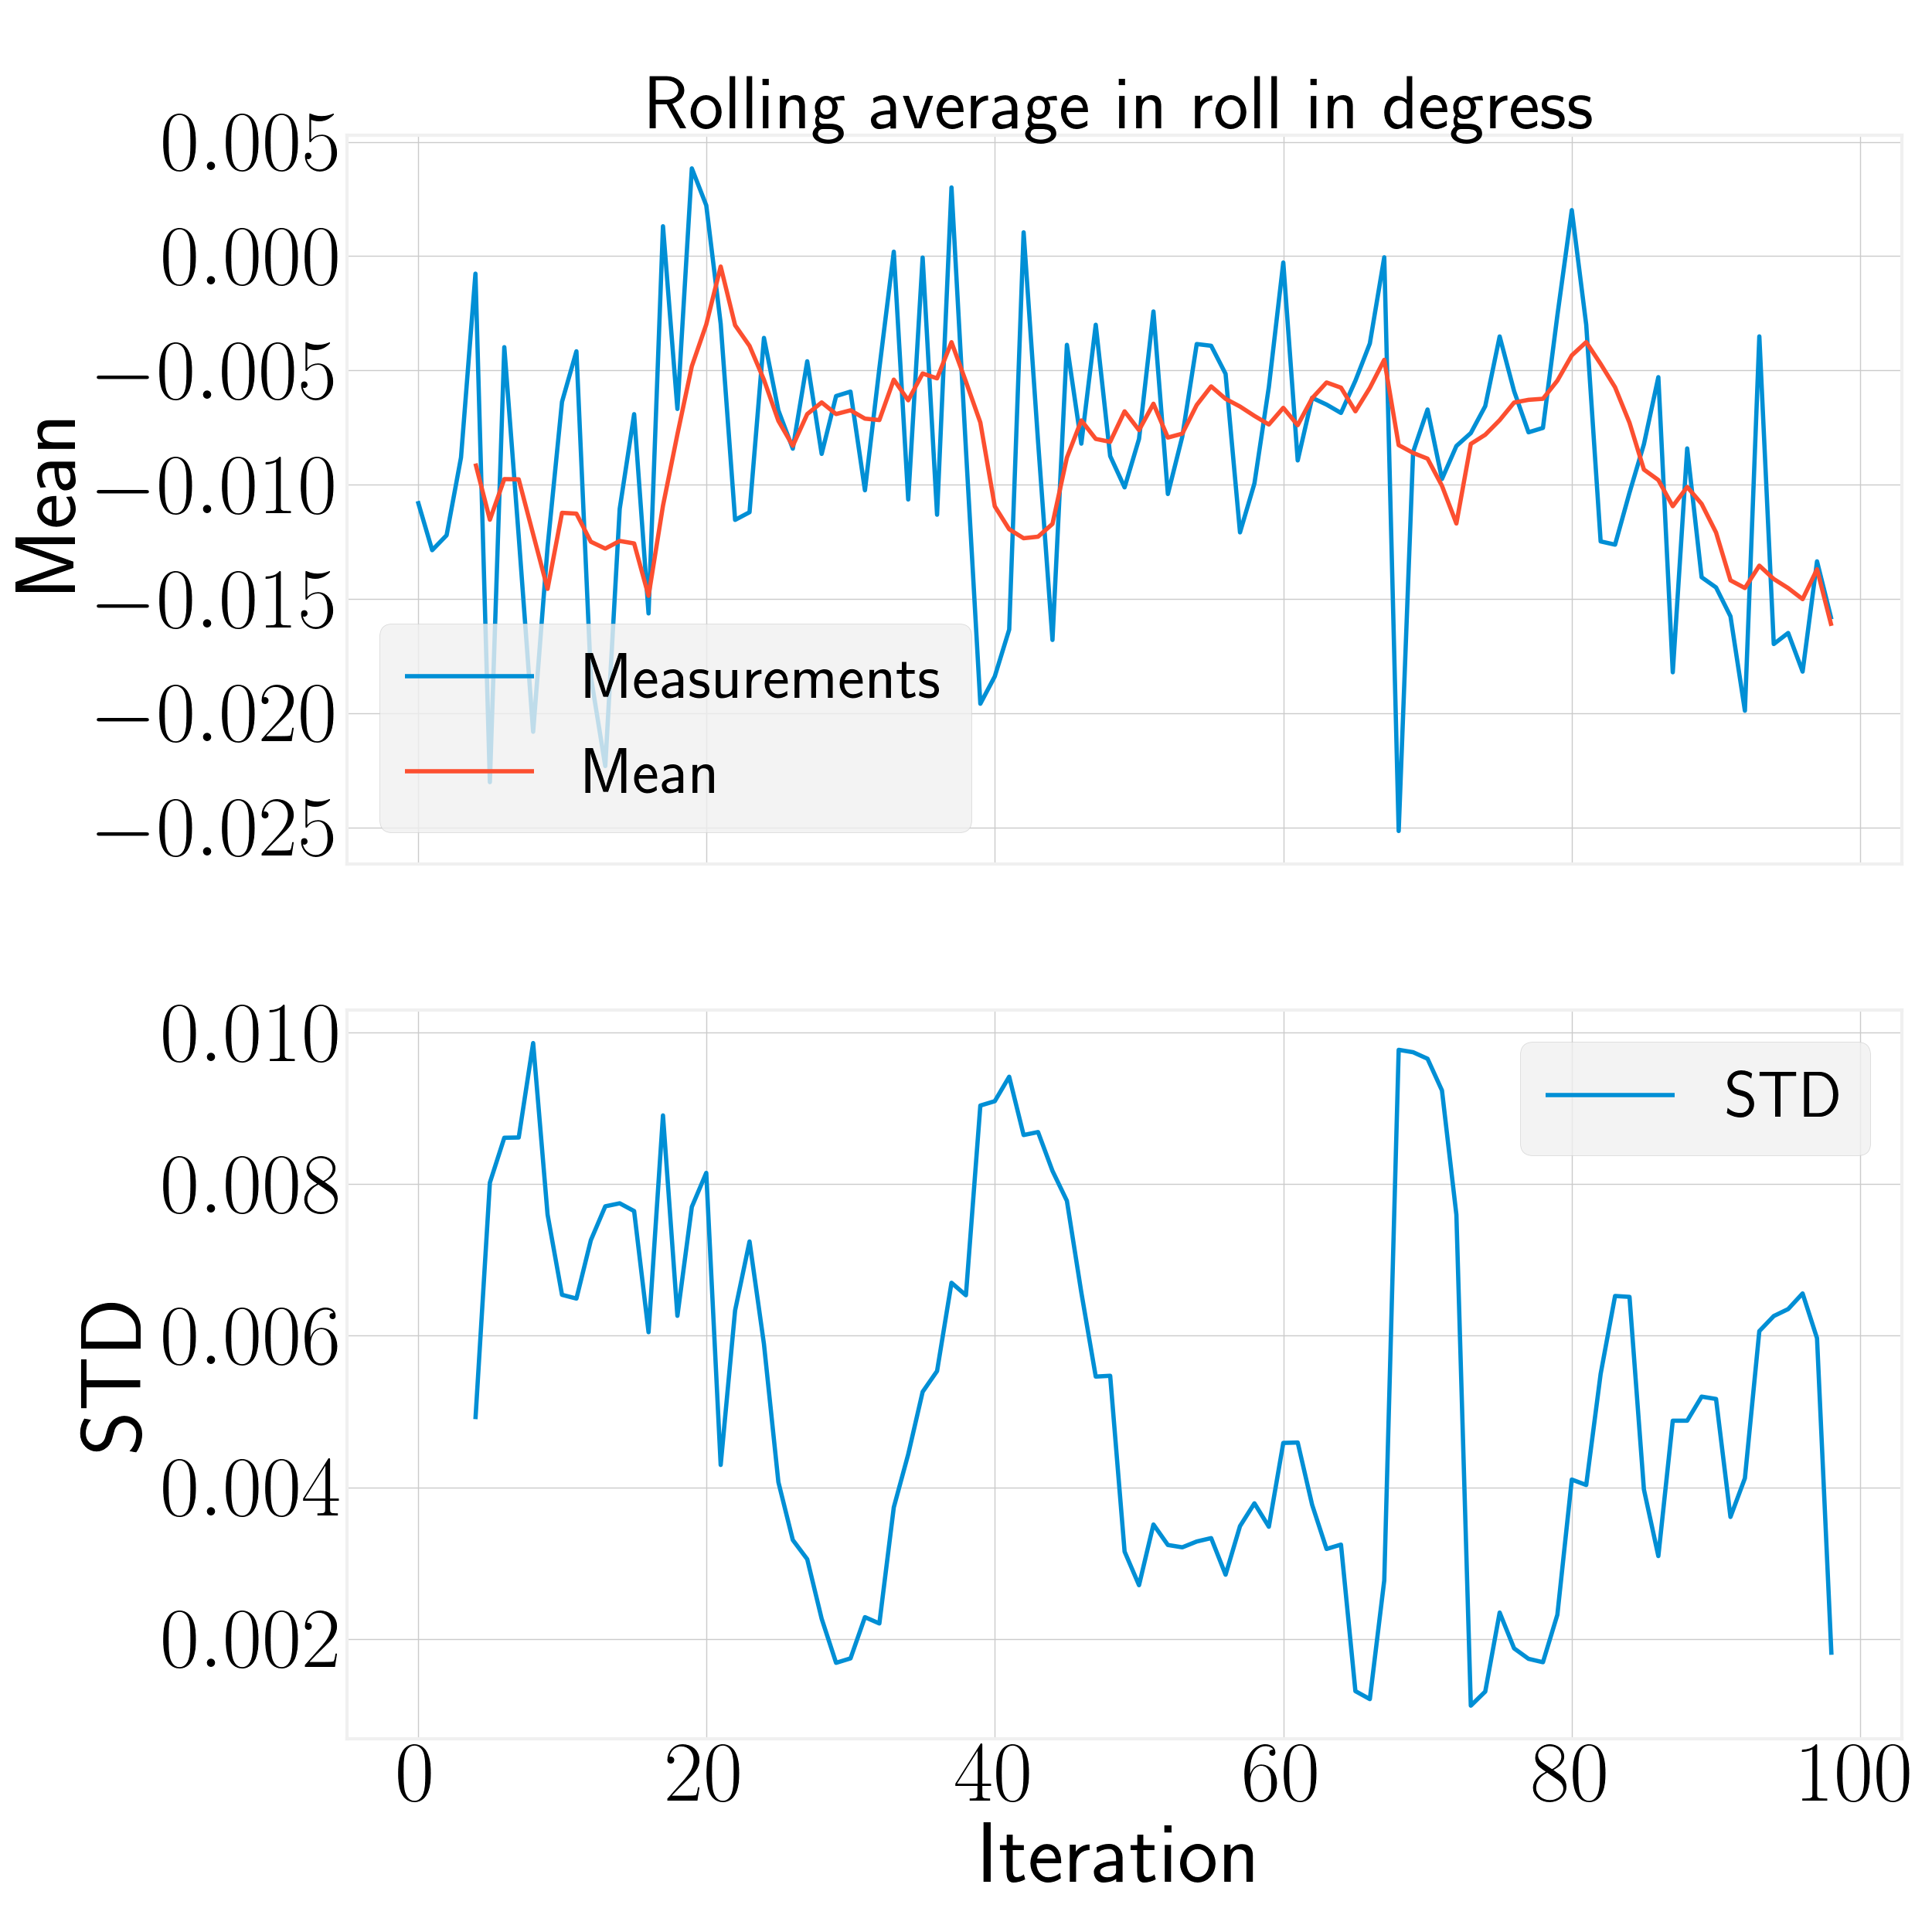
\includegraphics[width=\textwidth]{../Figures/analyse_rolling_average/test1/Calculated_rolling_average_in_roll_with_mean_and_STD.png}
        \caption{}
        \label{fig:rolling_average_in_roll_test1}
    \end{subfigure}
     \hspace{0.2em}
    \begin{subfigure}[t]{.30\textwidth}
        \centering
        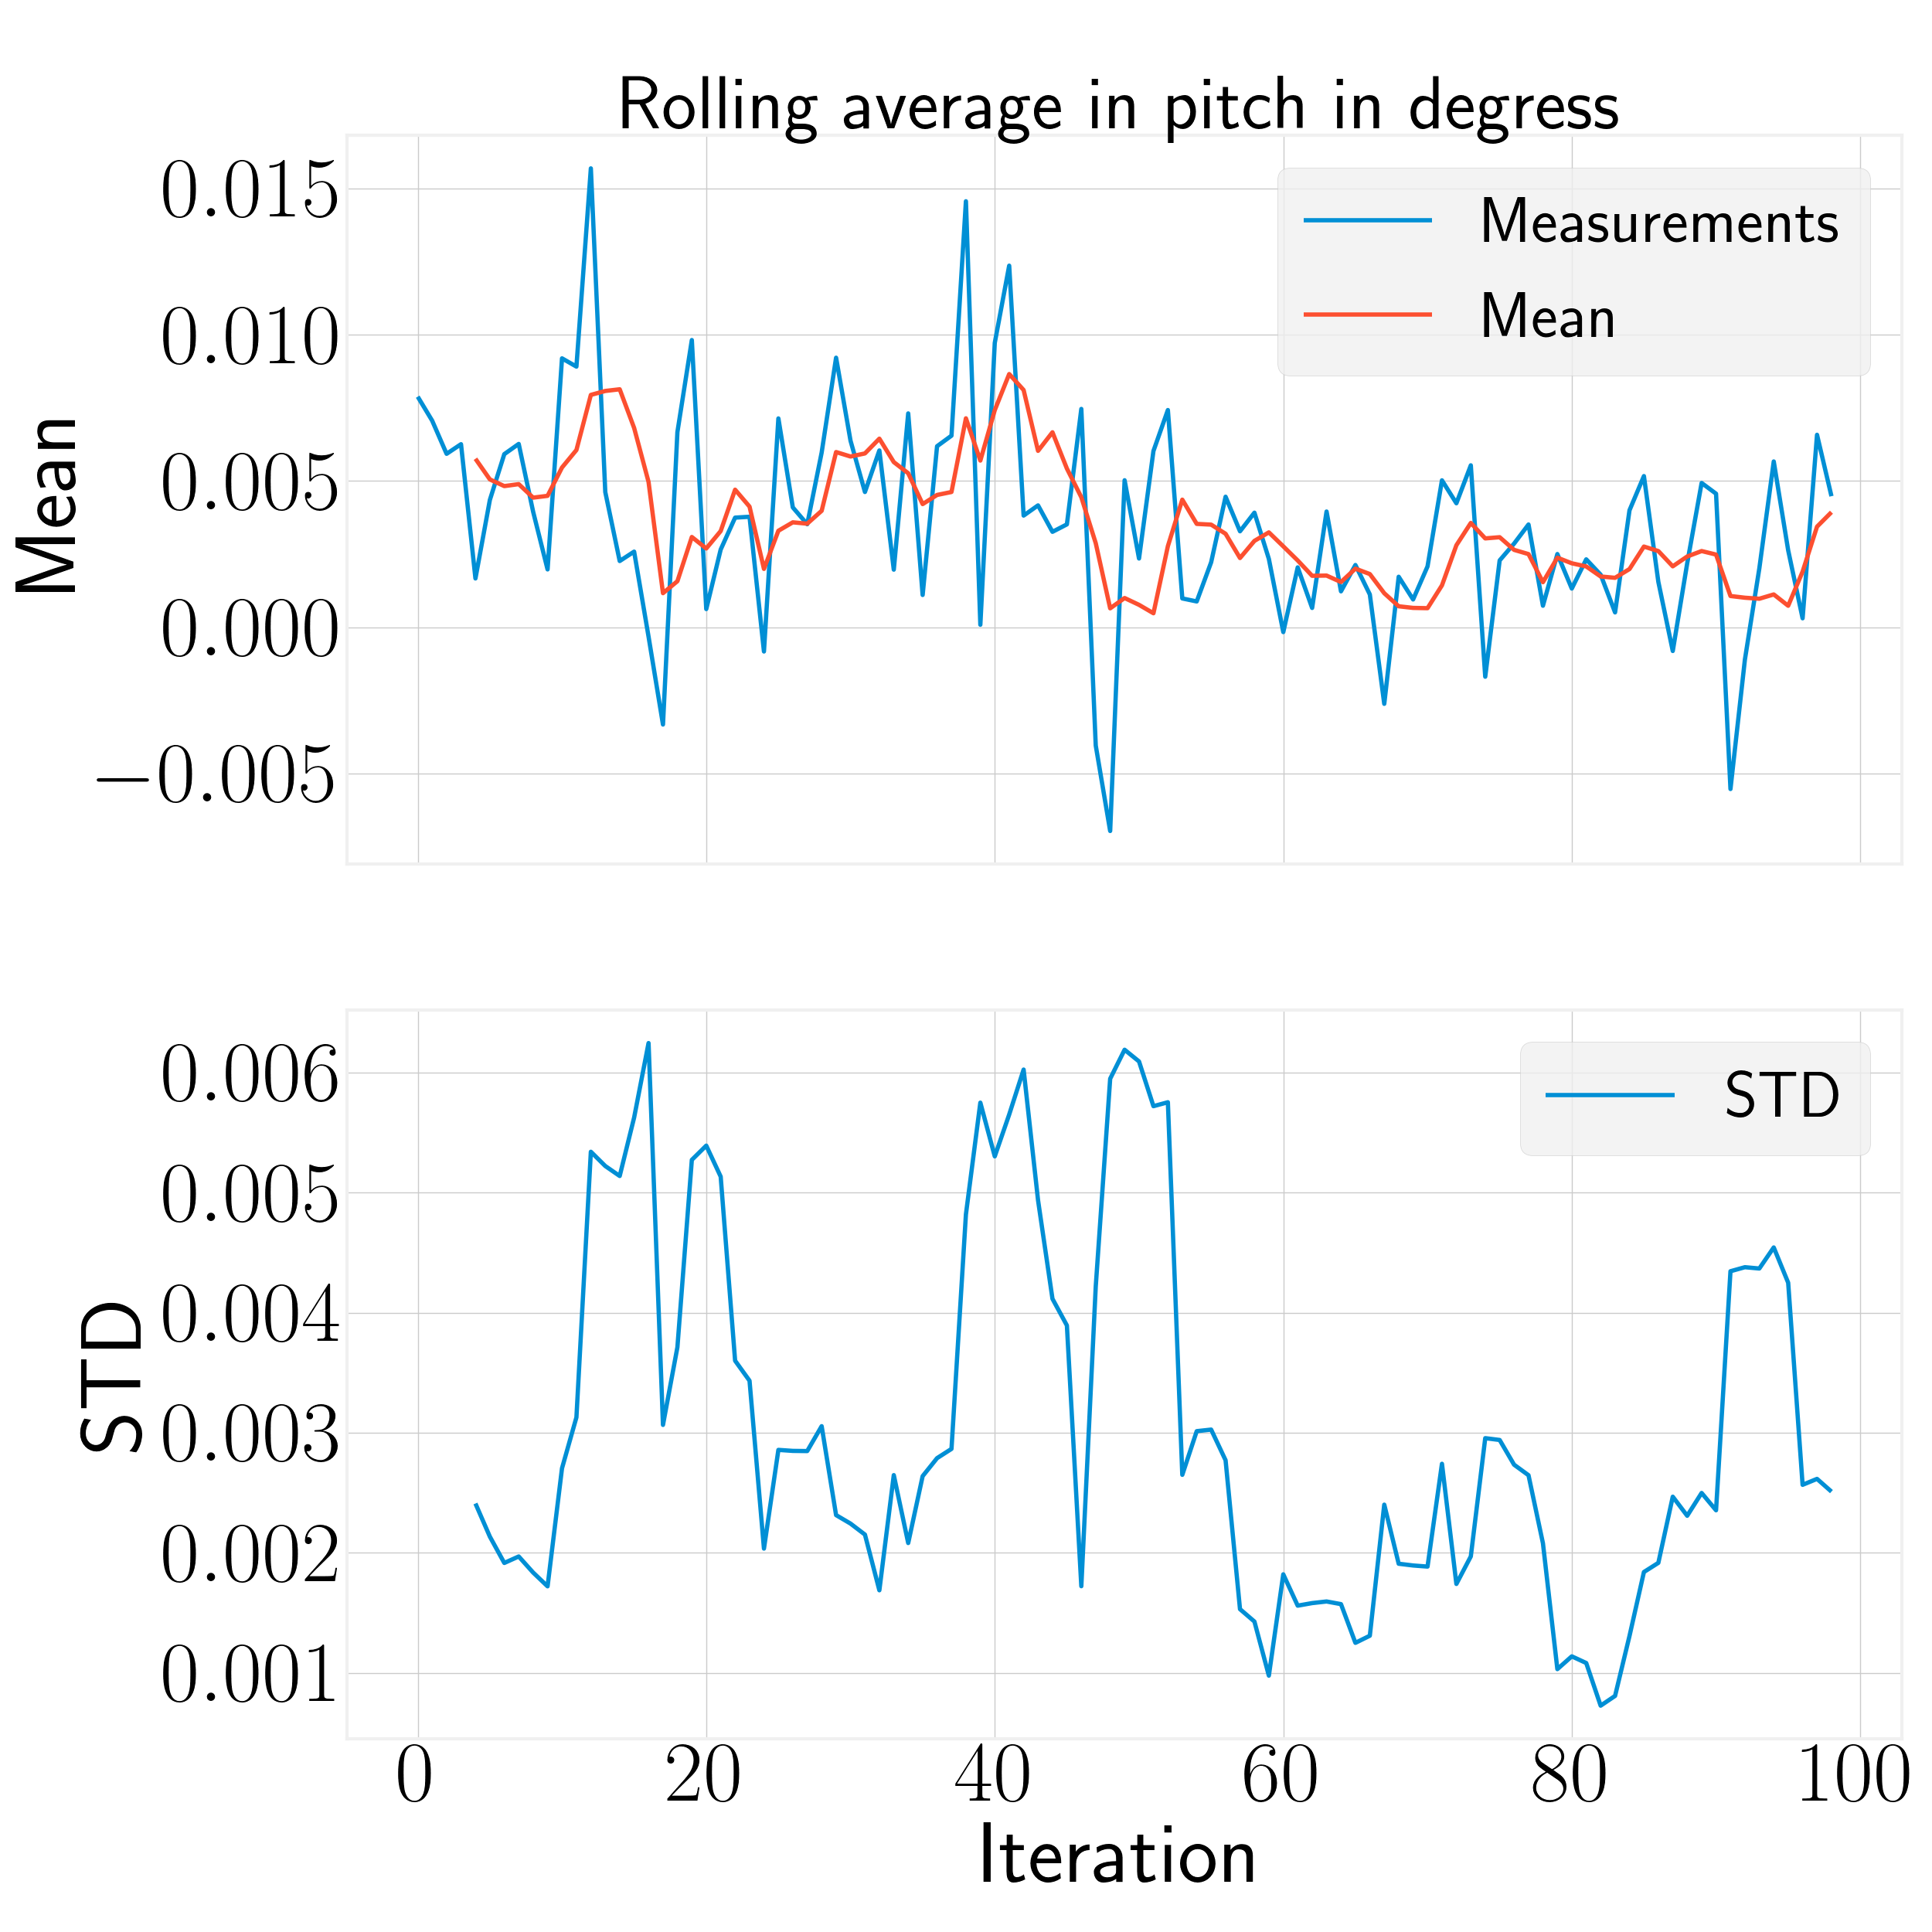
\includegraphics[width=\textwidth]{../Figures/analyse_rolling_average/test1/Calculated_rolling_average_in_pitch_with_mean_and_STD.png}
        \caption{}
        \label{fig:rolling_average_in_pitch_test1}
    \end{subfigure}
     \hspace{0.2em}
    \begin{subfigure}[t]{.30\textwidth}
        \centering
        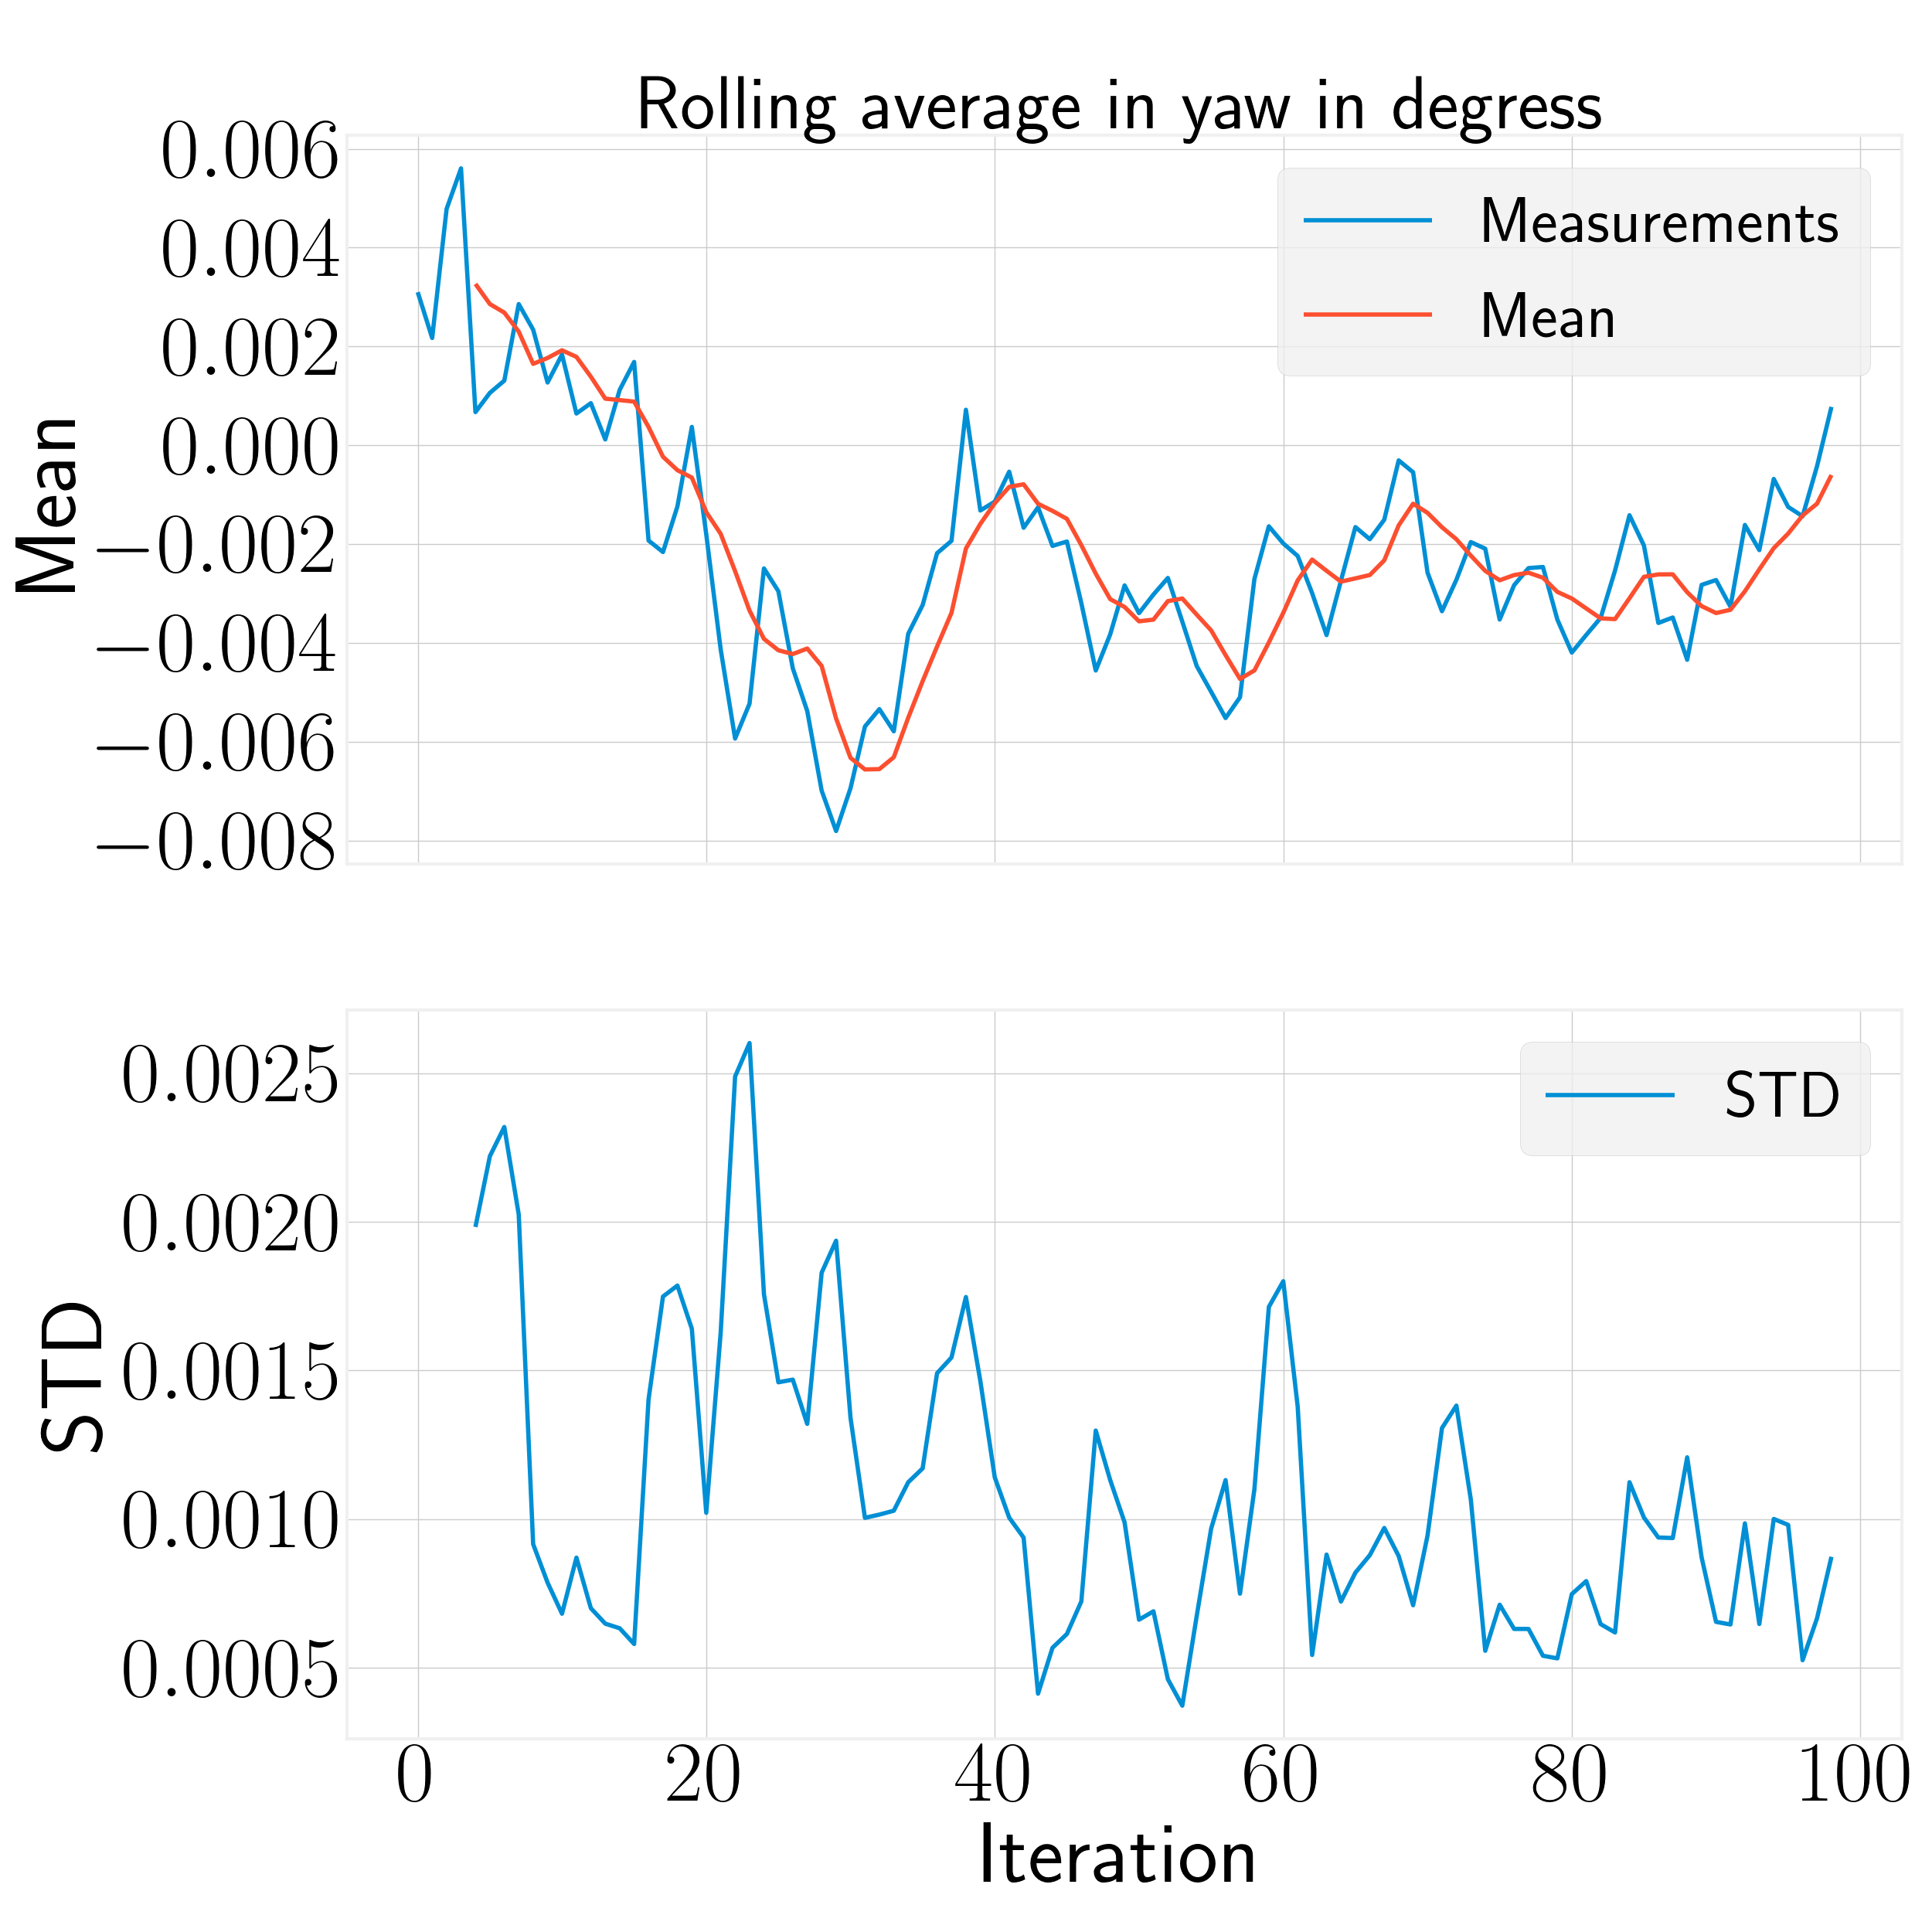
\includegraphics[width=\textwidth]{../Figures/analyse_rolling_average/test1/Calculated_rolling_average_in_yaw_with_mean_and_STD.png}
        \caption{}
        \label{fig:rolling_average_in_yaw_test1}
    \end{subfigure}
    \caption{Illustrations of the rolling average from the configuration in Figure \ref{fig:rolling_average_good_pos}. As it can be seen, the fluctuations in the angle estimates are steady with only negligible deviations}
    \label{fig:rolling_average_angle_test1}
\end{figure}

\begin{figure}[H]
    \centering
    \begin{subfigure}[t]{.30\textwidth}
        \centering
        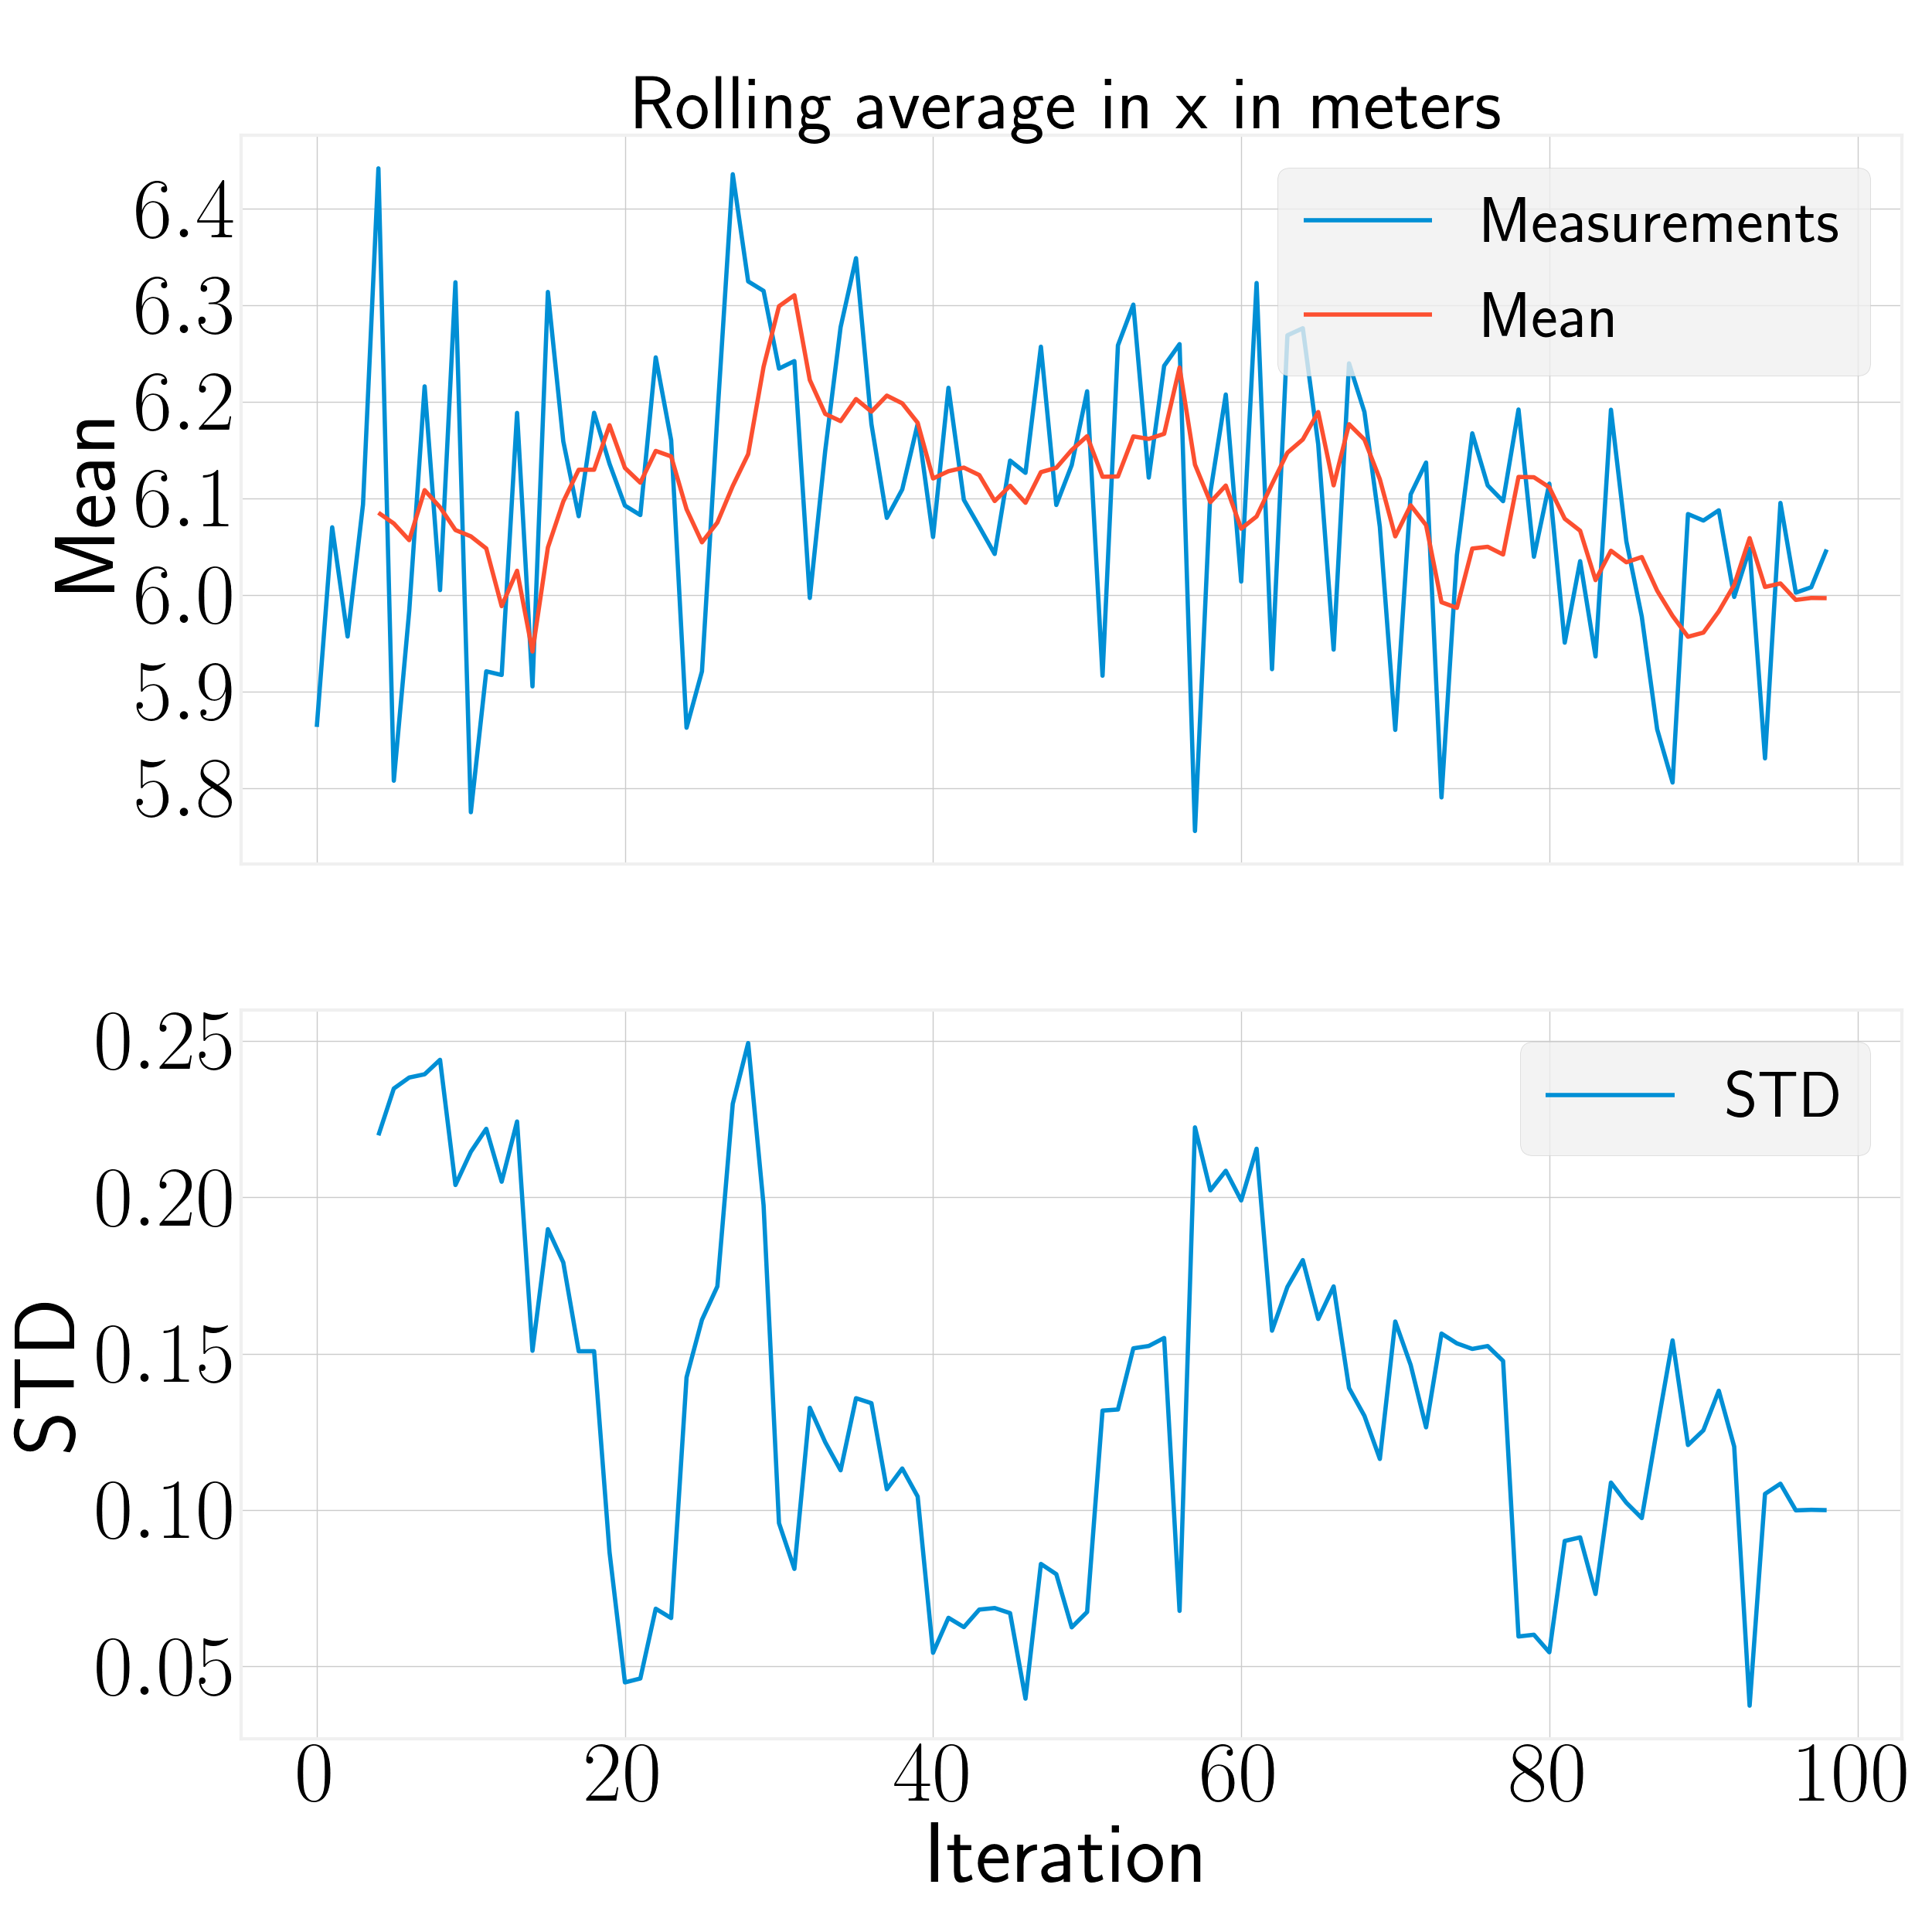
\includegraphics[width=\textwidth]{../Figures/analyse_rolling_average/test2/Calculated_rolling_average_in_x_with_mean_and_STD.png}
        \caption{}
        \label{fig:rolling_average_in_x_test2}
    \end{subfigure}
     \hspace{0.2em}
    \begin{subfigure}[t]{.30\textwidth}
        \centering
        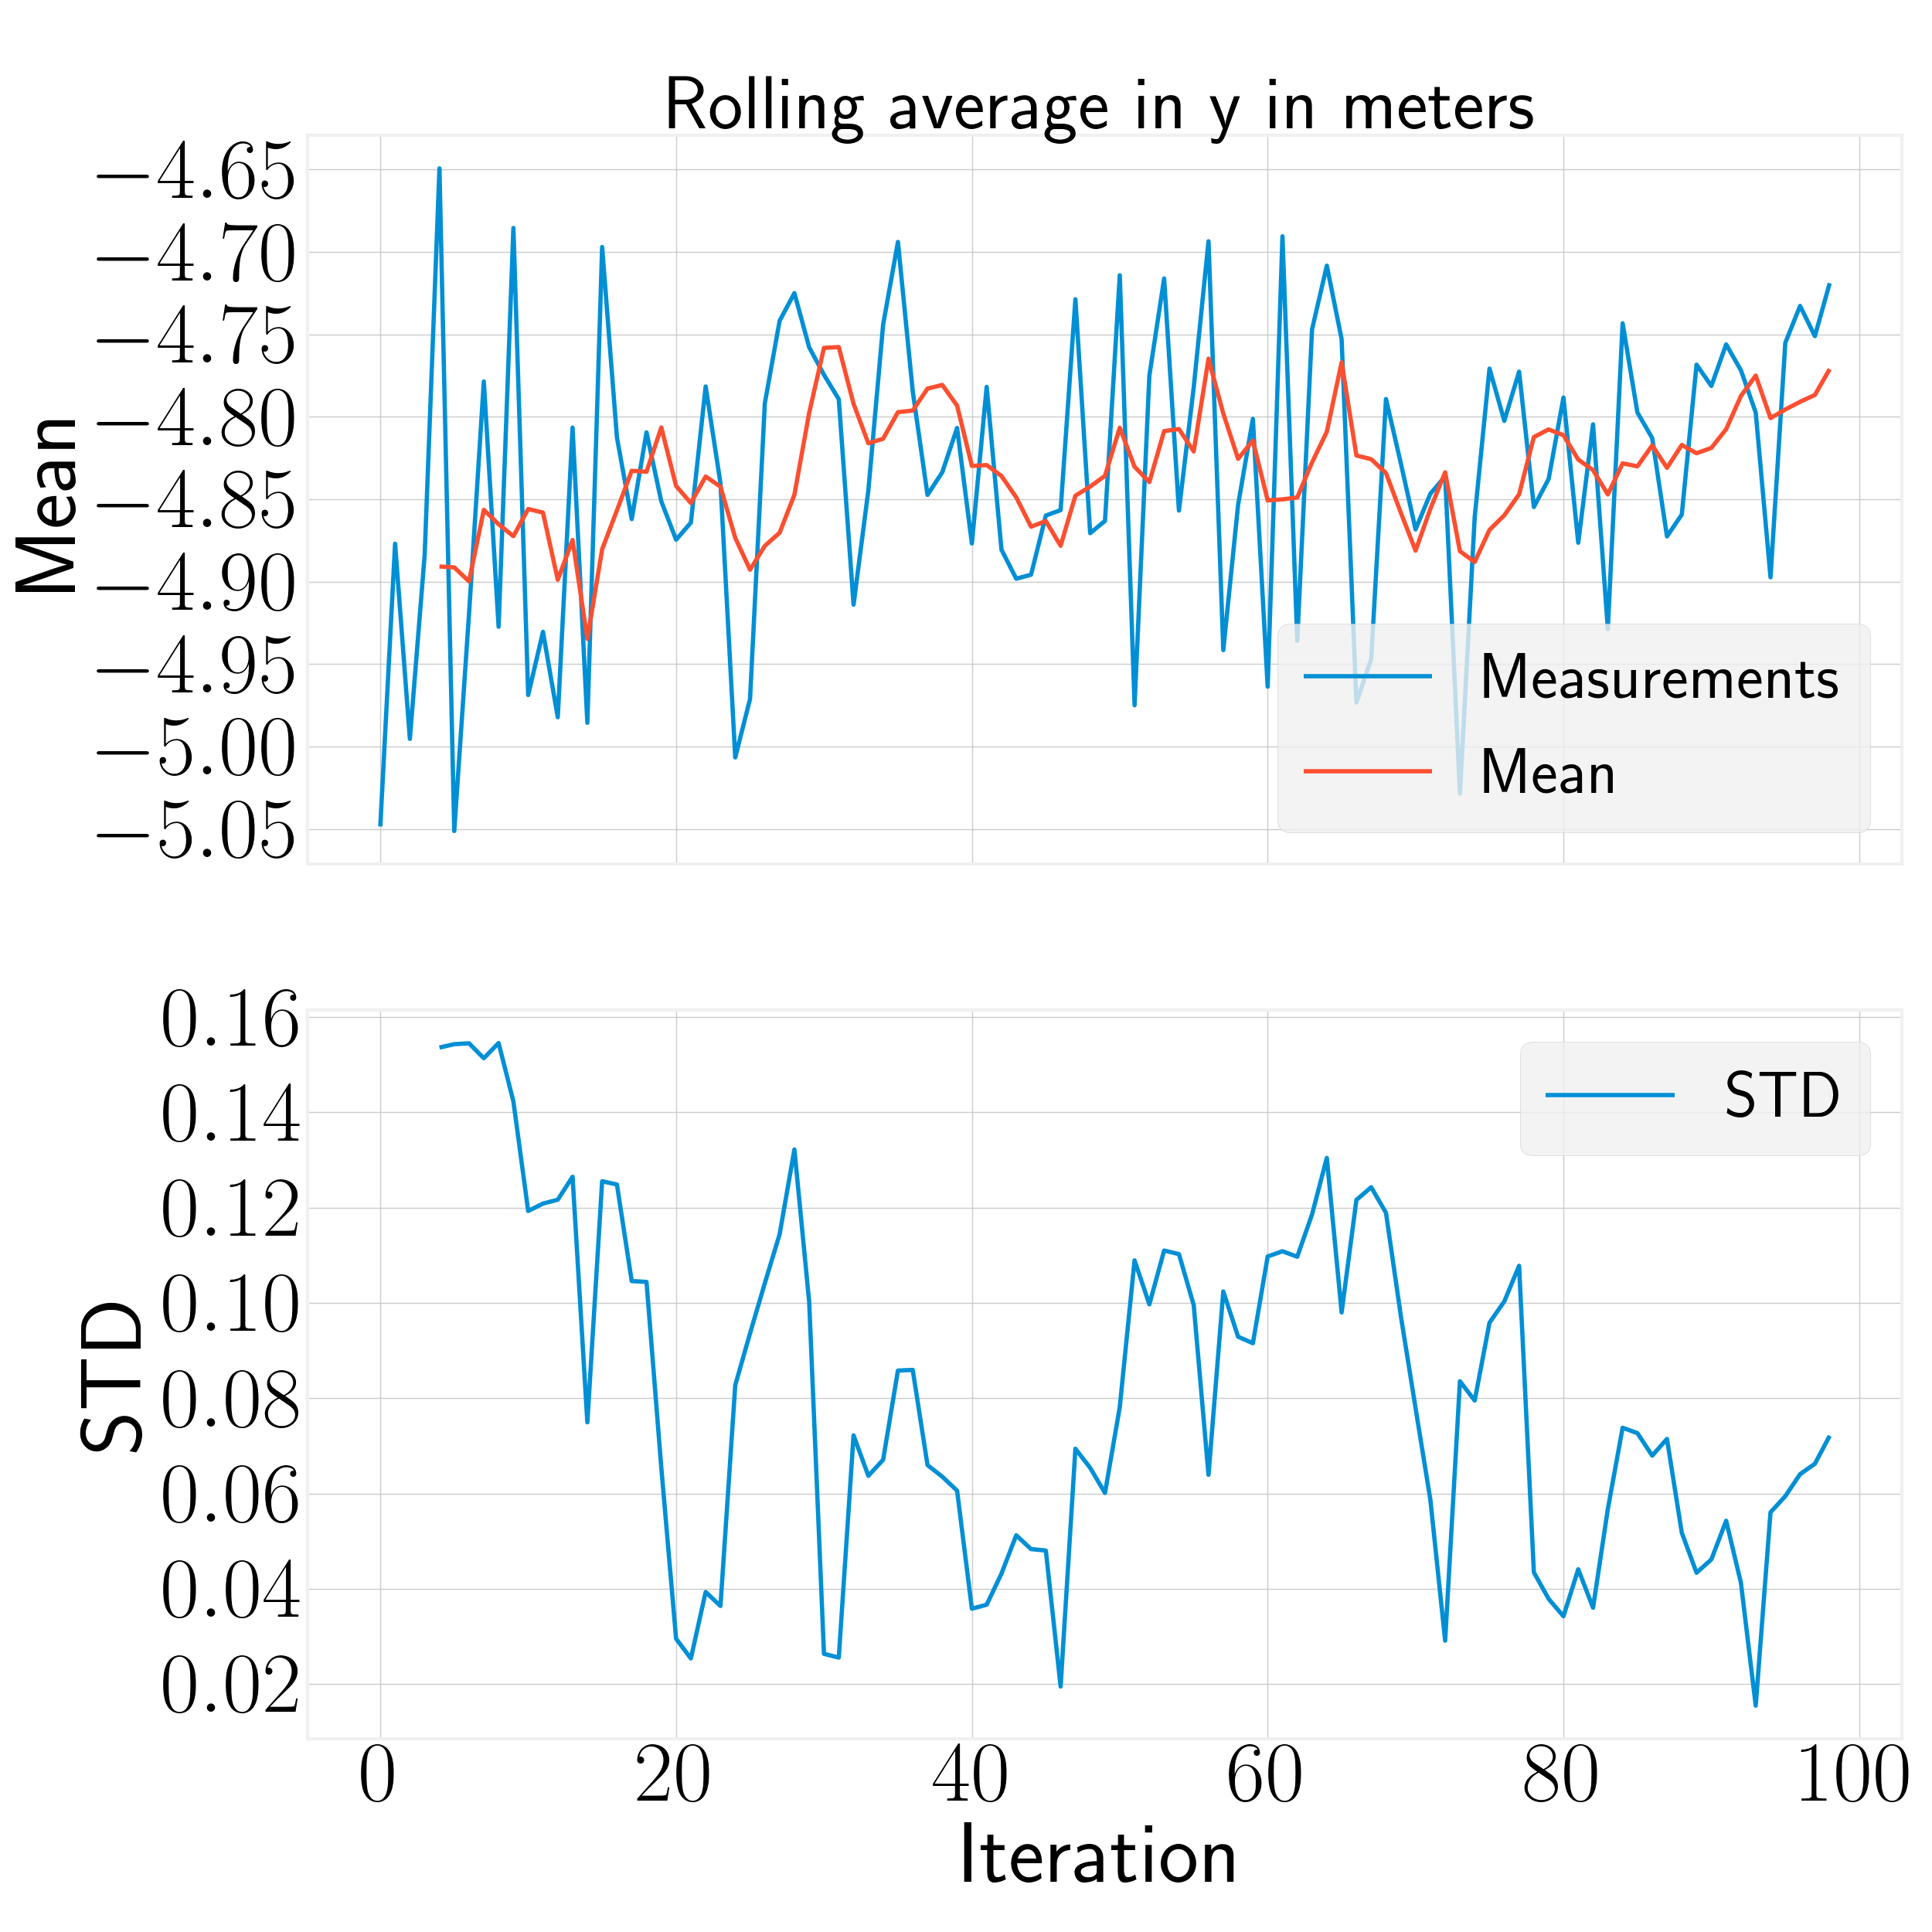
\includegraphics[width=\textwidth]{../Figures/analyse_rolling_average/test2/Calculated_rolling_average_in_y_with_mean_and_STD.png}
        \caption{}
        \label{fig:rolling_average_in_y_test2}
    \end{subfigure}
     \hspace{0.2em}
    \begin{subfigure}[t]{.30\textwidth}
        \centering
        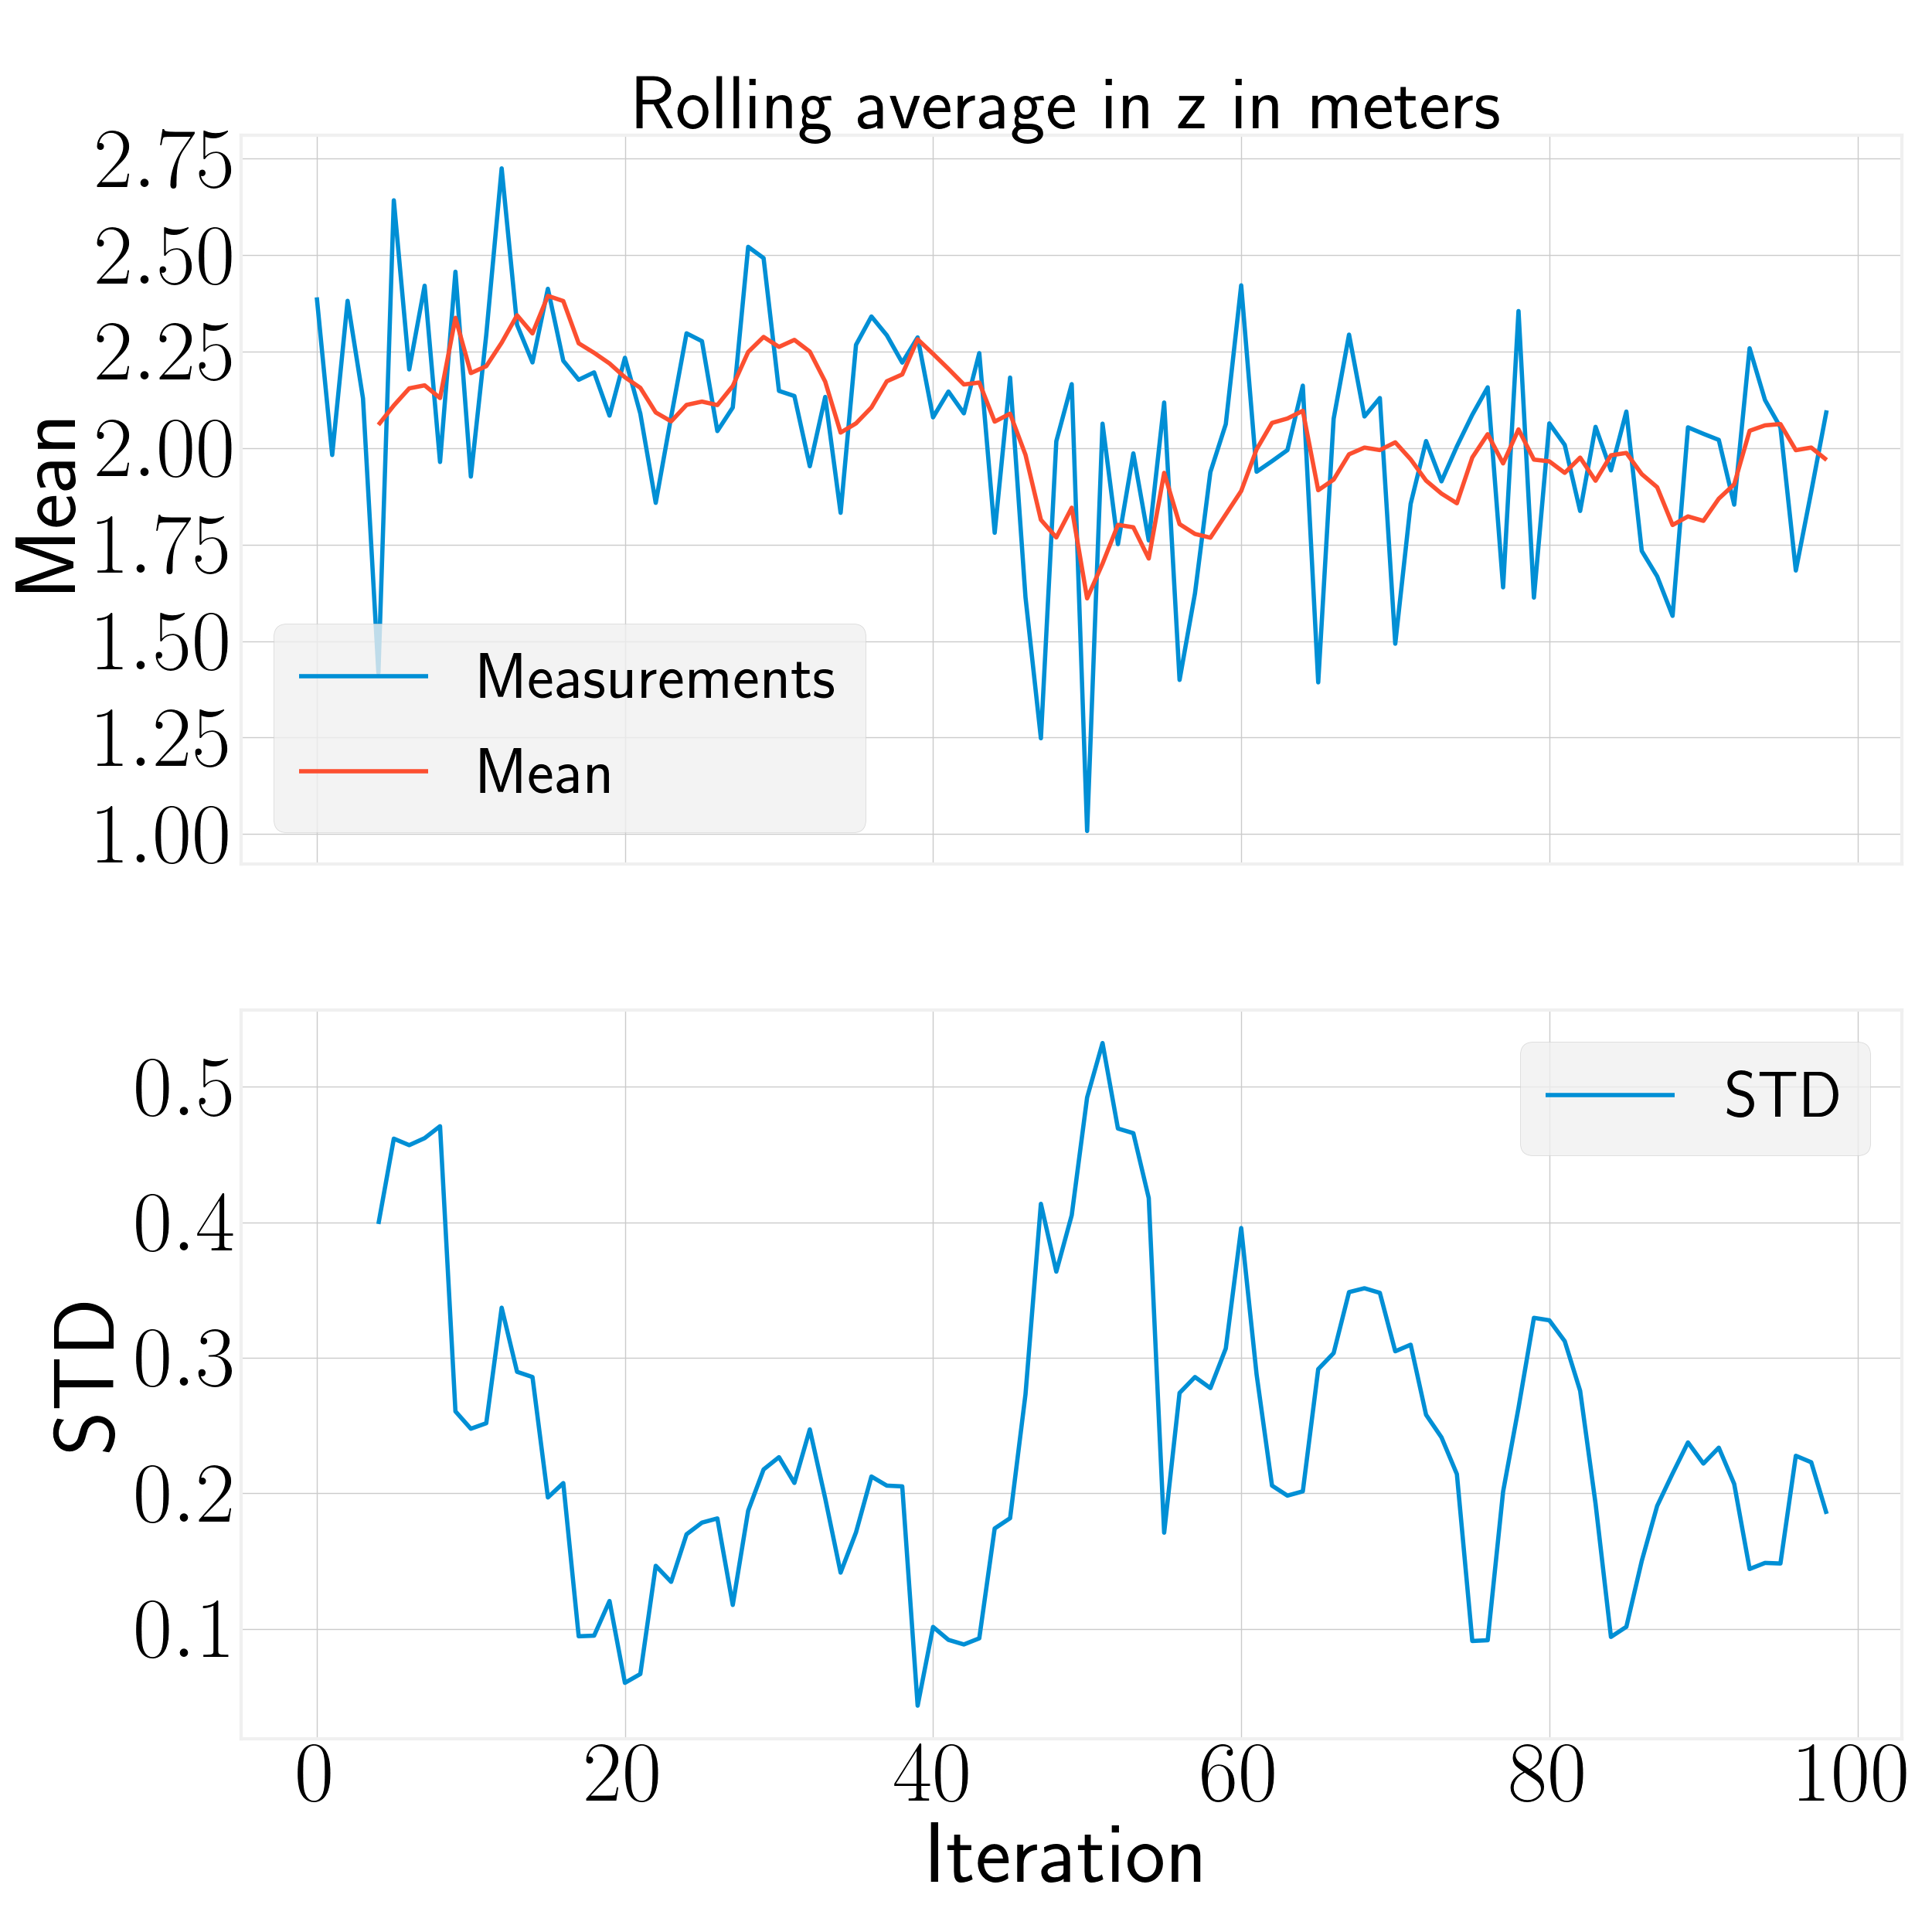
\includegraphics[width=\textwidth]{../Figures/analyse_rolling_average/test2/Calculated_rolling_average_in_z_with_mean_and_STD.png}
        \caption{}
        \label{fig:rolling_average_in_z_test2}
    \end{subfigure}
    \caption{Illustrations of the rolling average from the configuration in Figure \ref{fig:rolling_average_bad_pos}. As it can be seen, the fluctuations of the position estimates fluctuates a lot especially in the altitude}
    \label{fig:rolling_average_pos_test2}
\end{figure}

\begin{figure}[H]
    \centering
    \begin{subfigure}[t]{.30\textwidth}
        \centering
        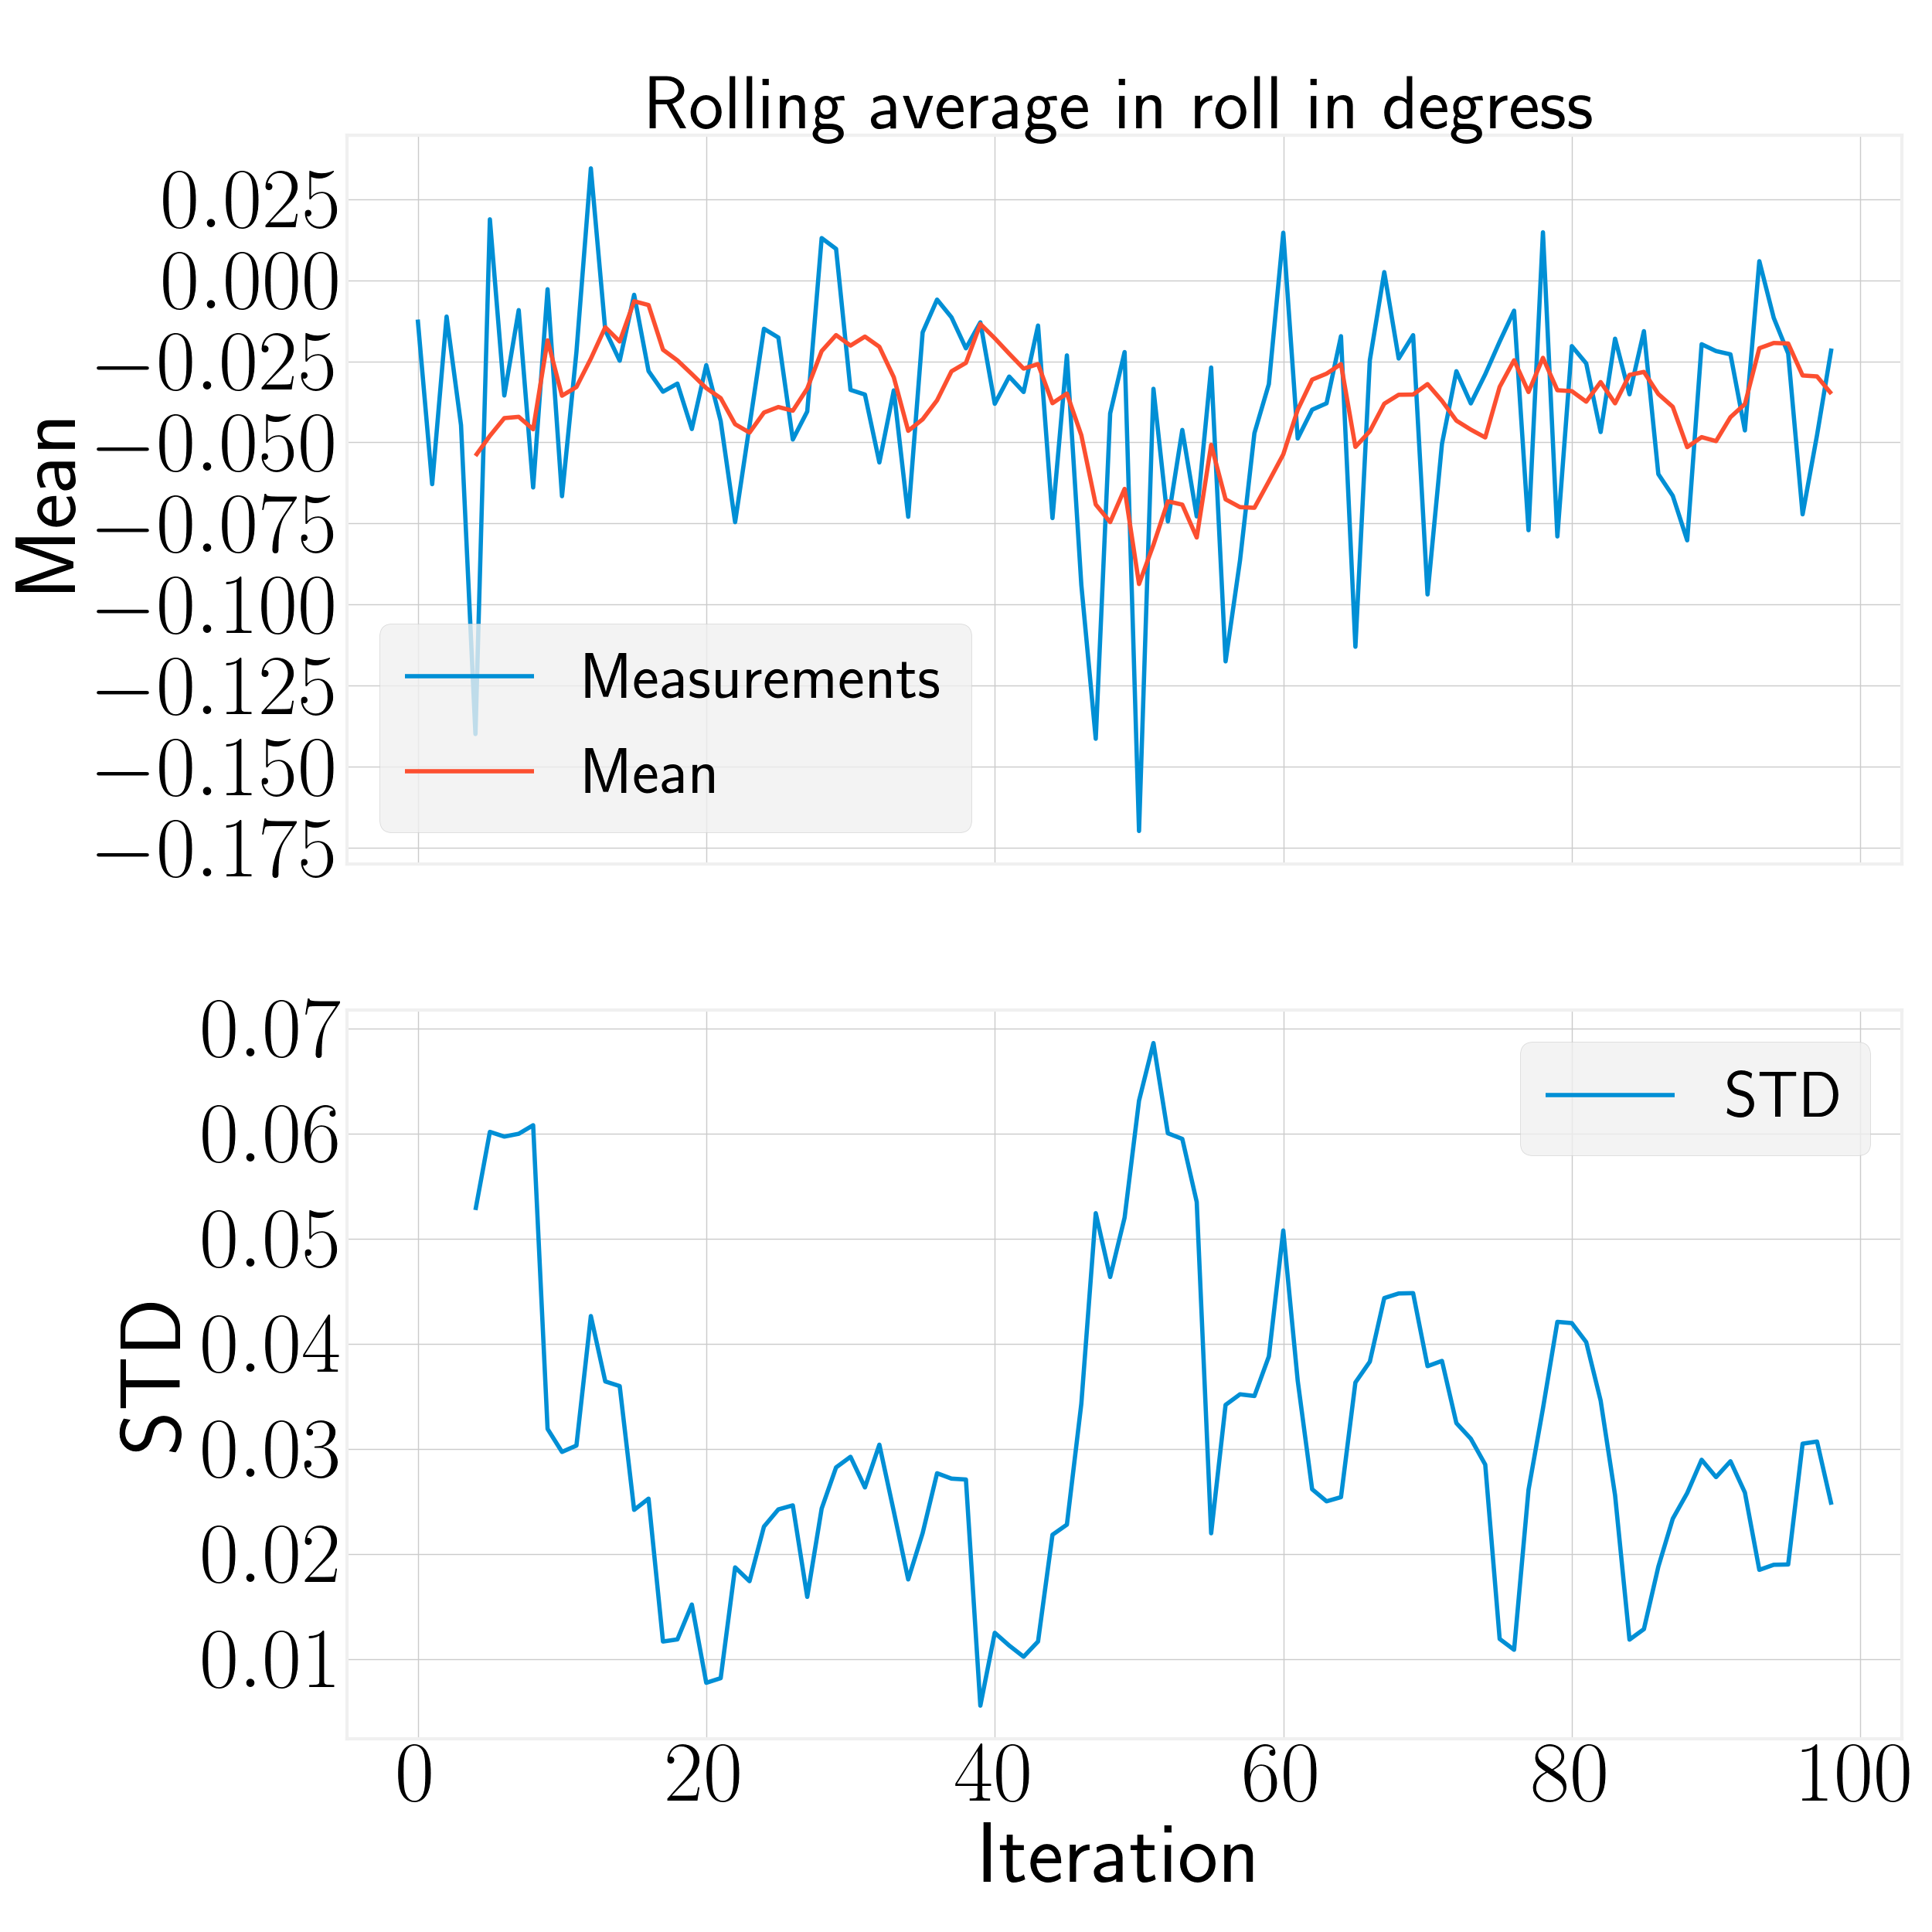
\includegraphics[width=\textwidth]{../Figures/analyse_rolling_average/test2/Calculated_rolling_average_in_roll_with_mean_and_STD.png}
        \caption{}
        \label{fig:rolling_average_in_roll_test2}
    \end{subfigure}
     \hspace{0.2em}
    \begin{subfigure}[t]{.30\textwidth}
        \centering
        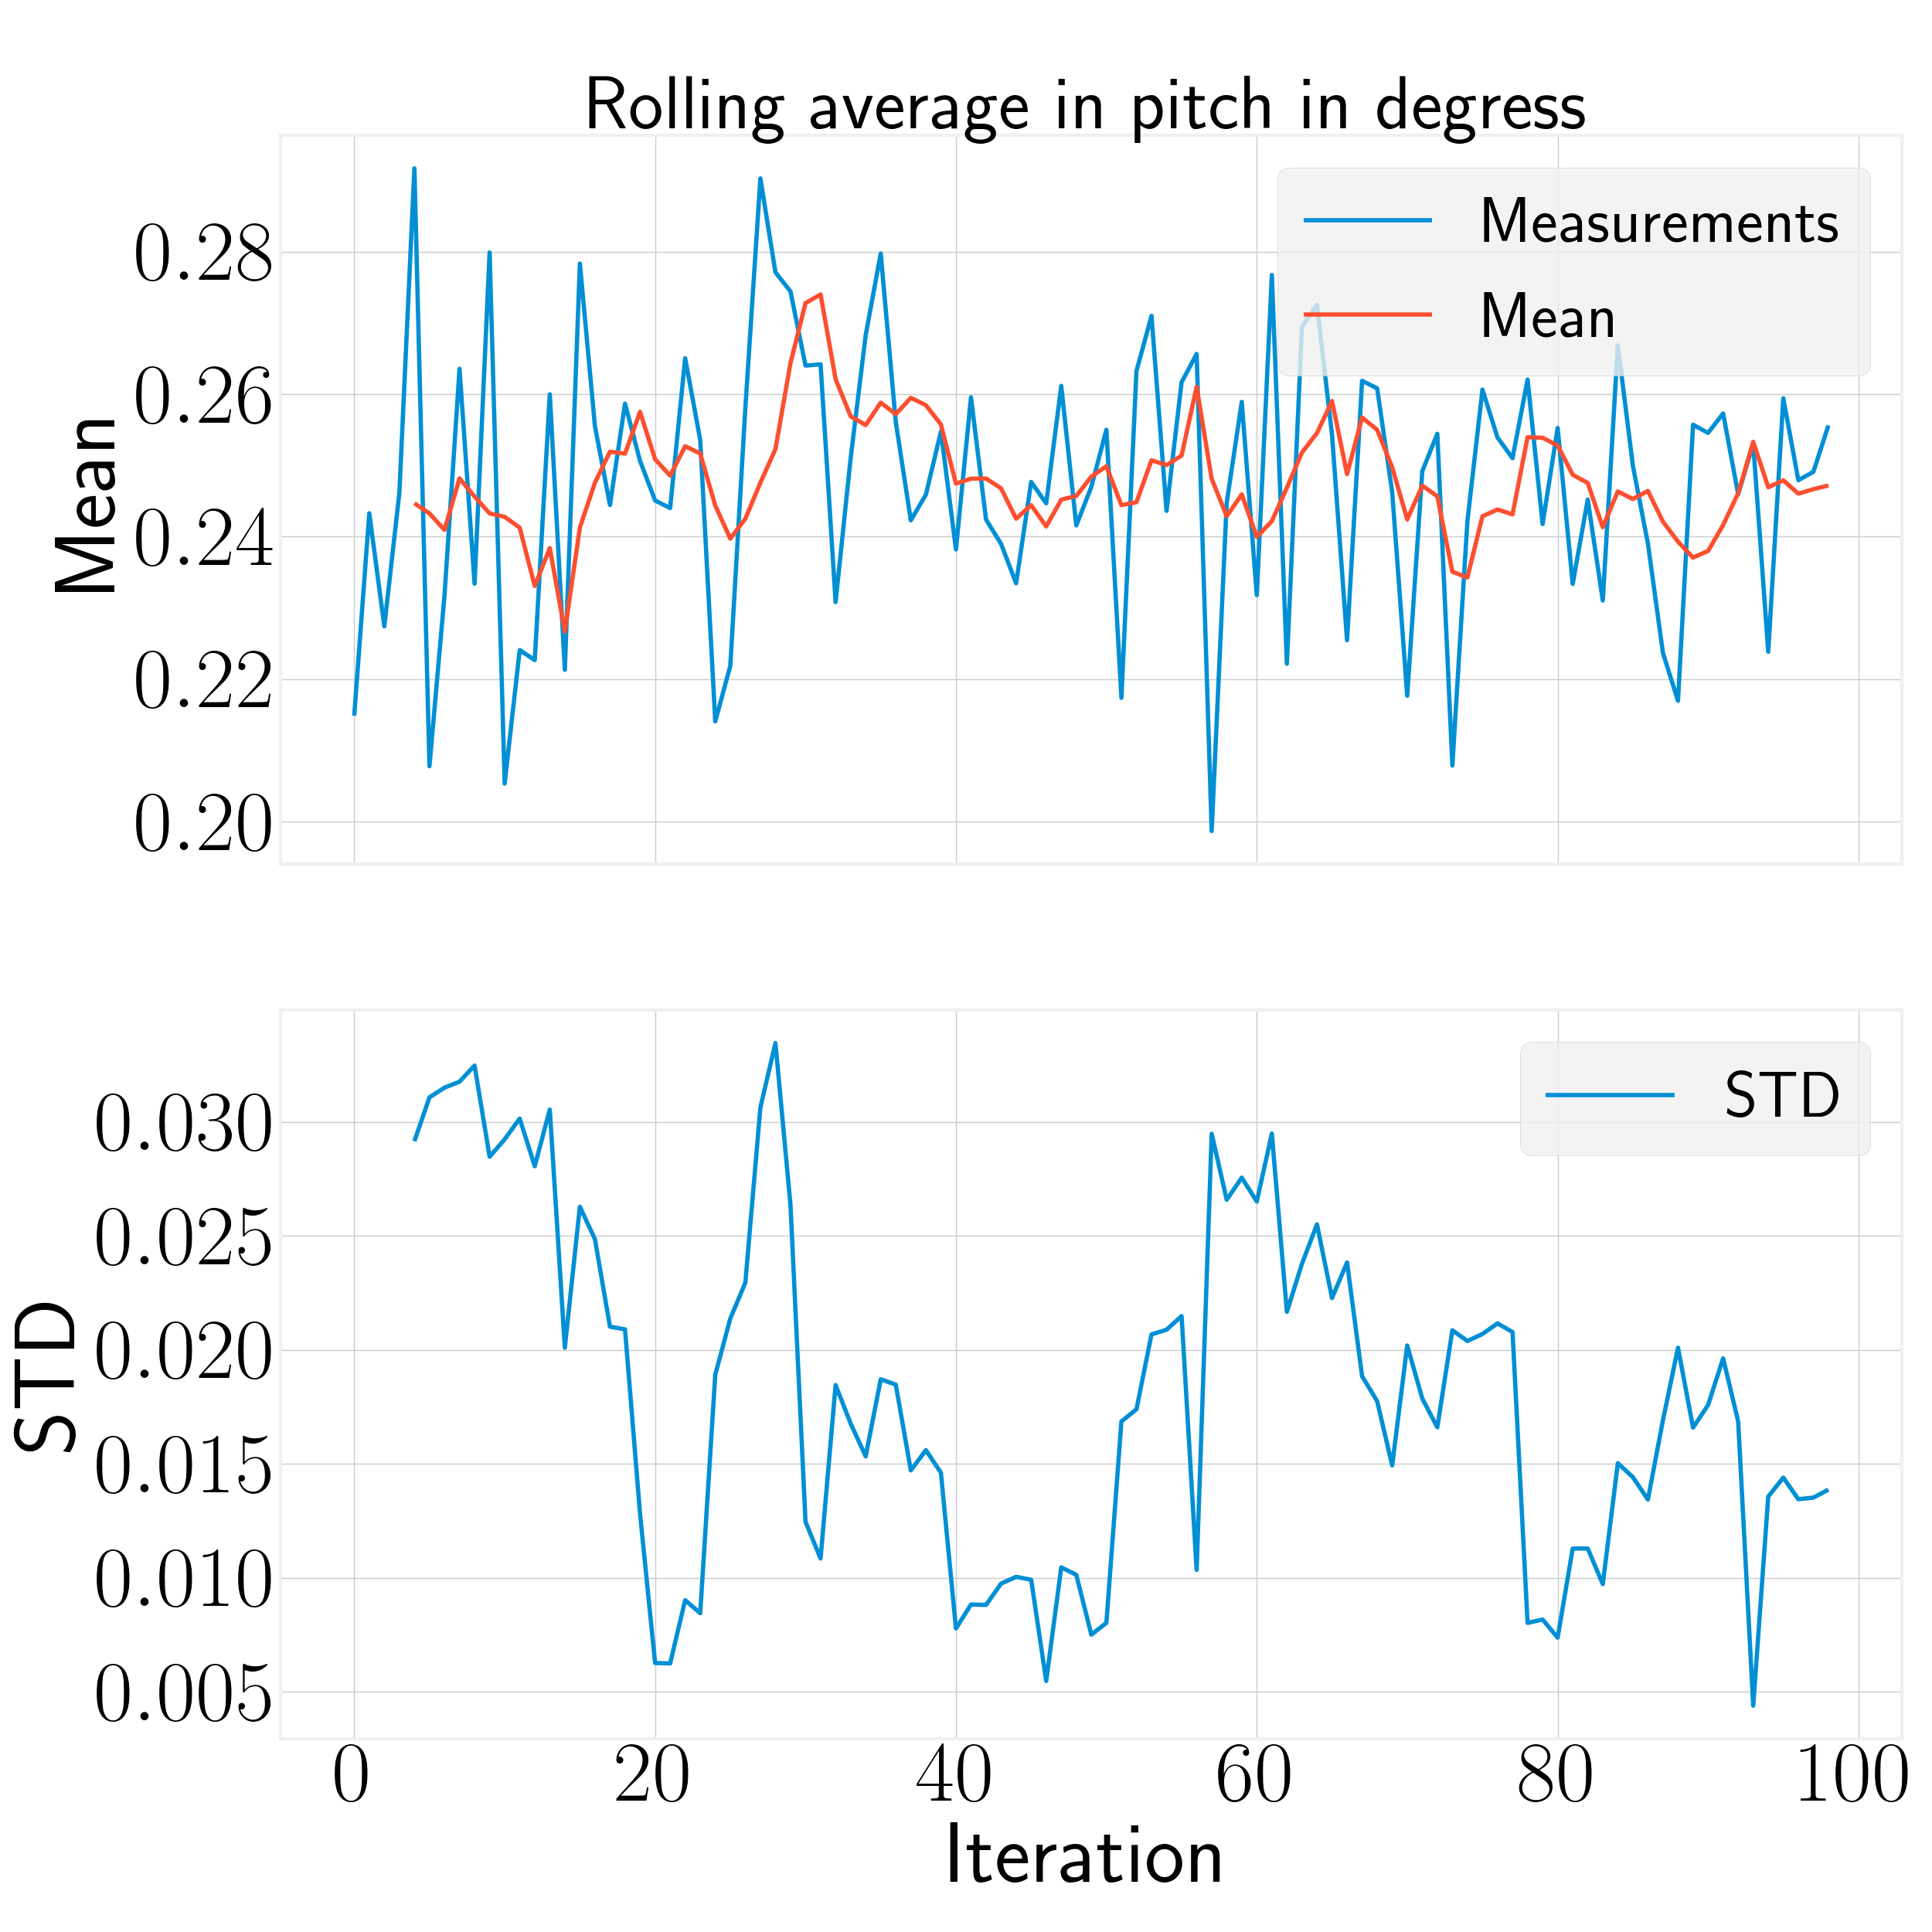
\includegraphics[width=\textwidth]{../Figures/analyse_rolling_average/test2/Calculated_rolling_average_in_pitch_with_mean_and_STD.png}
        \caption{}
        \label{fig:rolling_average_in_pitch_test2}
    \end{subfigure}
     \hspace{0.2em}
    \begin{subfigure}[t]{.30\textwidth}
        \centering
        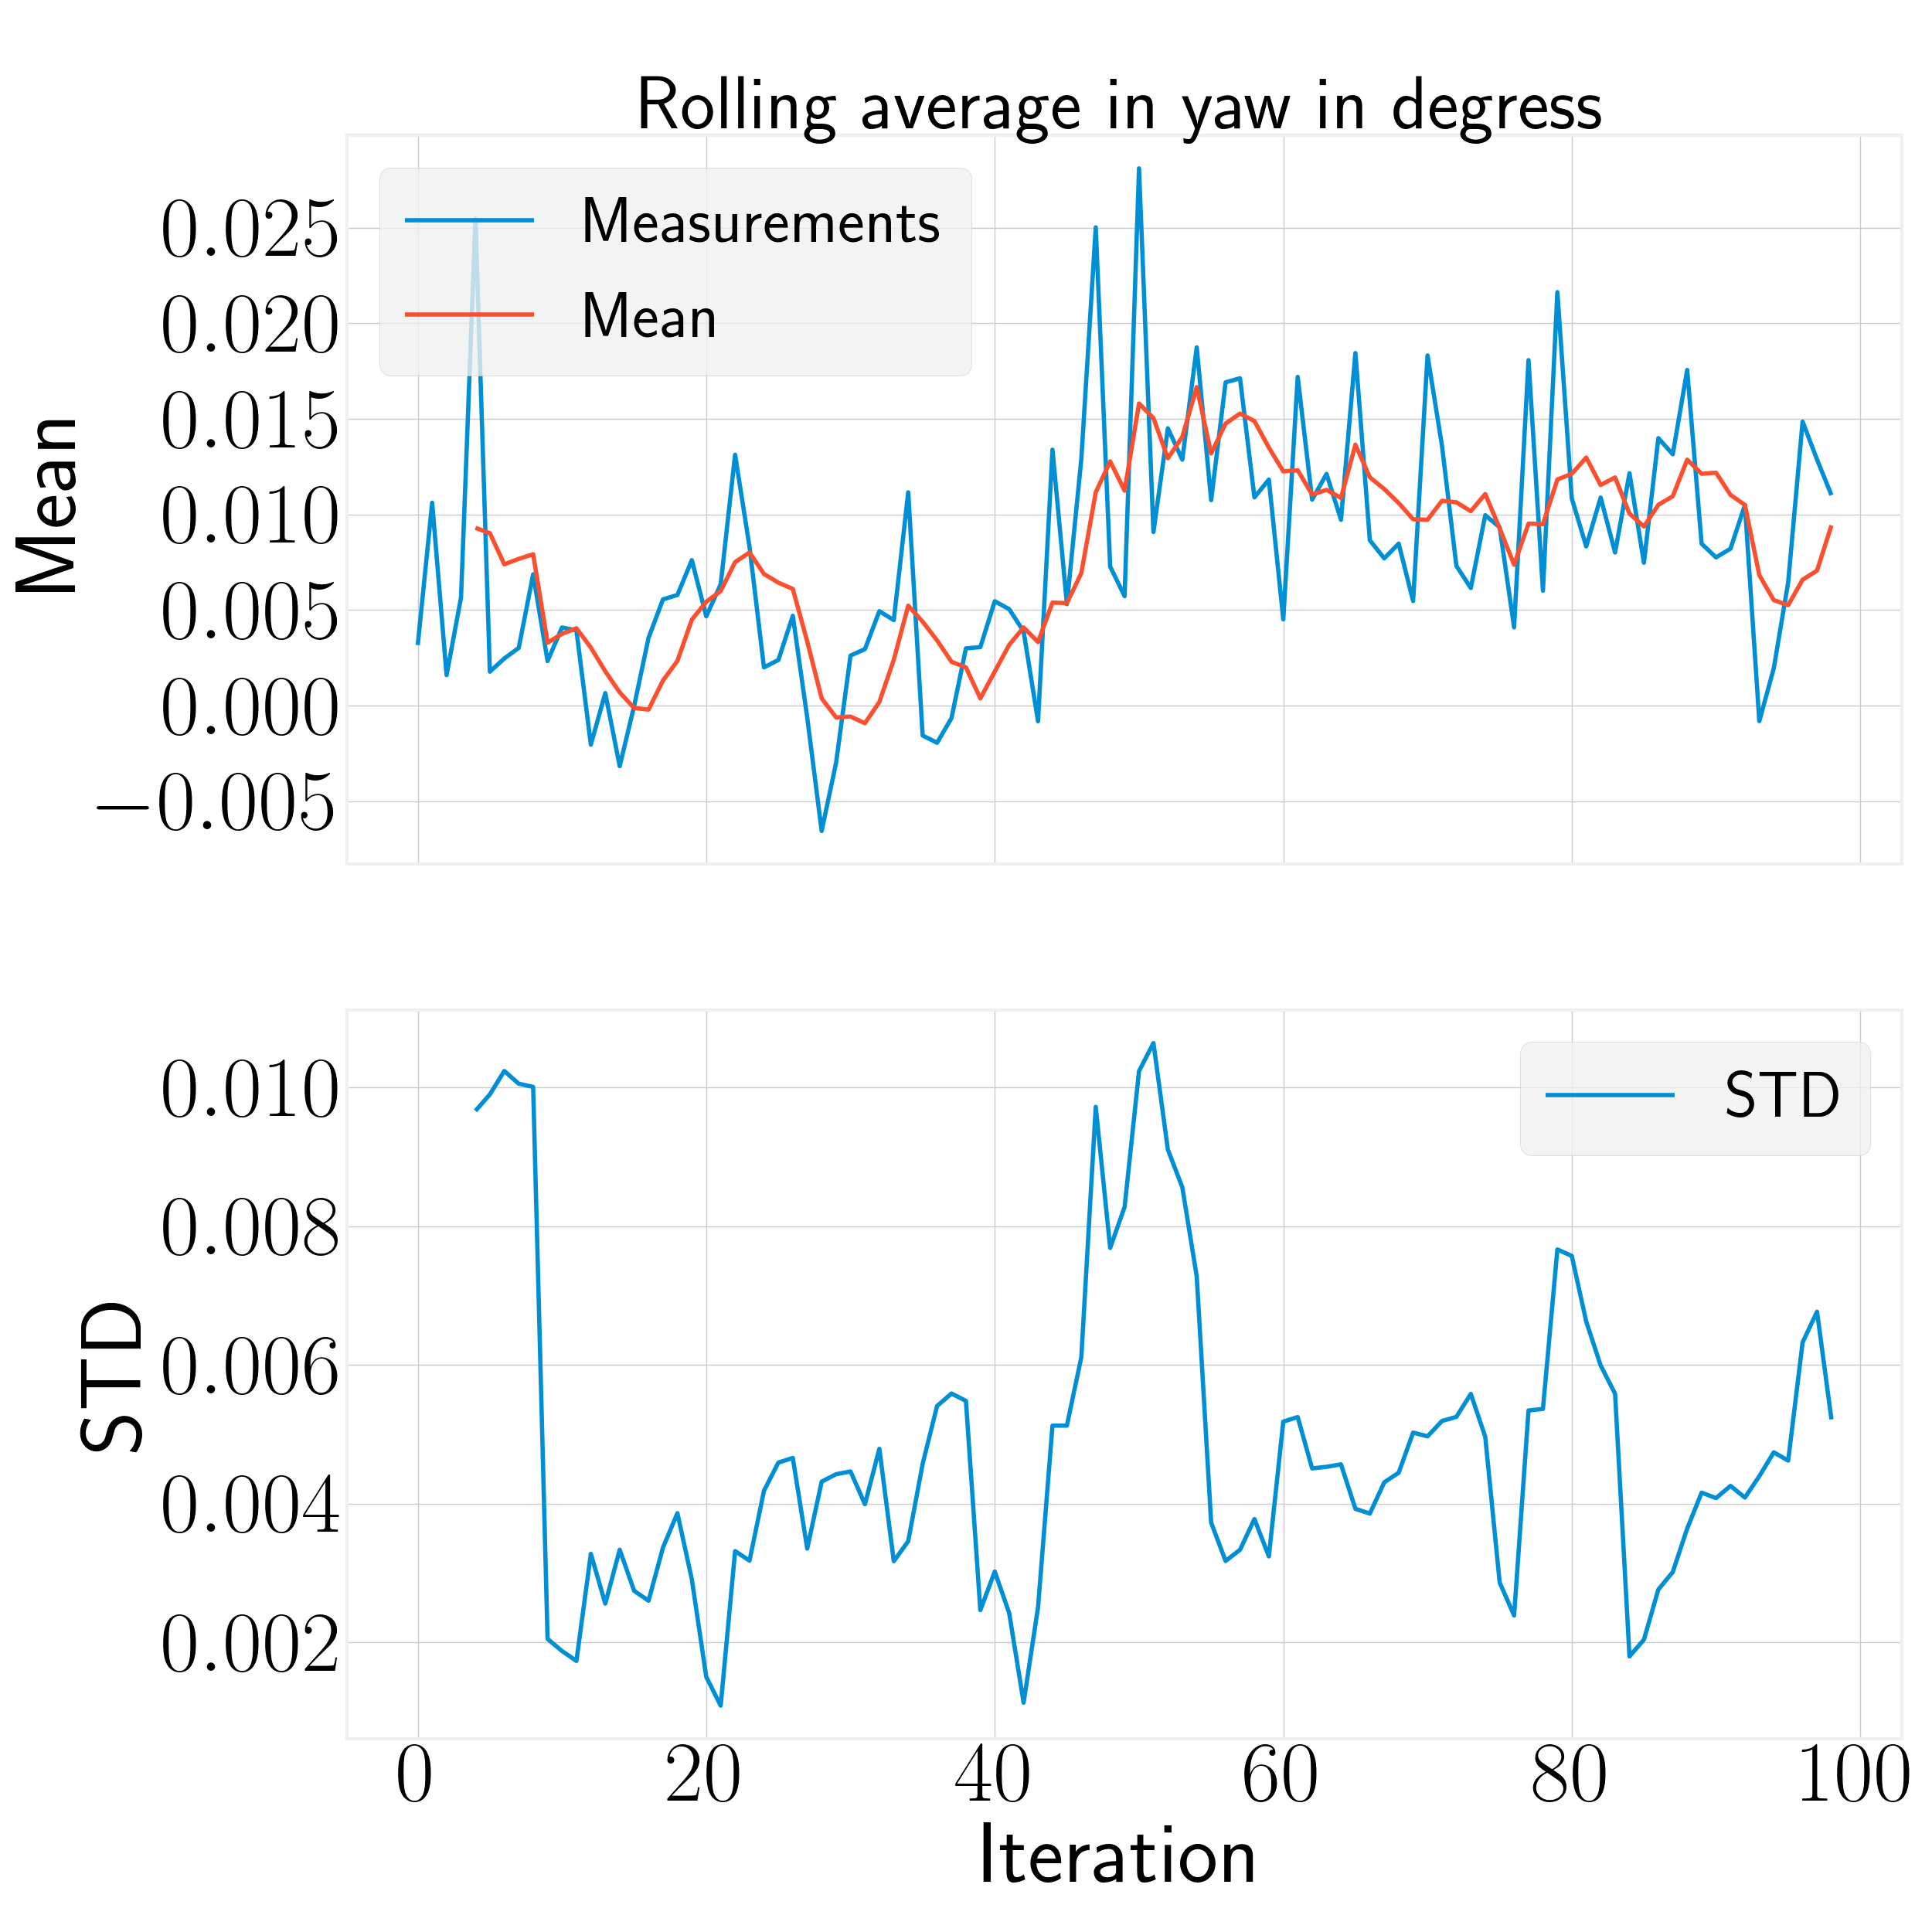
\includegraphics[width=\textwidth]{../Figures/analyse_rolling_average/test2/Calculated_rolling_average_in_yaw_with_mean_and_STD.png}
        \caption{}
        \label{fig:rolling_average_in_yaw_test2}
    \end{subfigure}
    \caption{Illustrations of the rolling average from the configuration in Figure \ref{fig:rolling_average_bad_pos}. As it can be seen, the fluctuations in the angle are steady even in this configuration}
    \label{fig:rolling_average_angle_test2}
\end{figure}  

This is done as an extension to the maximum allowed distance from the GPS2Vision marker from Section \ref{sec:GPS2Vision_pose_estimation} to insure that the GPS to vision transition is only performed when the pose estimates are stable and reliable. 

\subsubsection{Hold pose using ArUco pose estimation}
\label{sec:hold_pose_using_aruco_pose_estimation}

\begin{figure}[H]
    \centering
    \begin{subfigure}[t]{.30\textwidth}
        \centering
        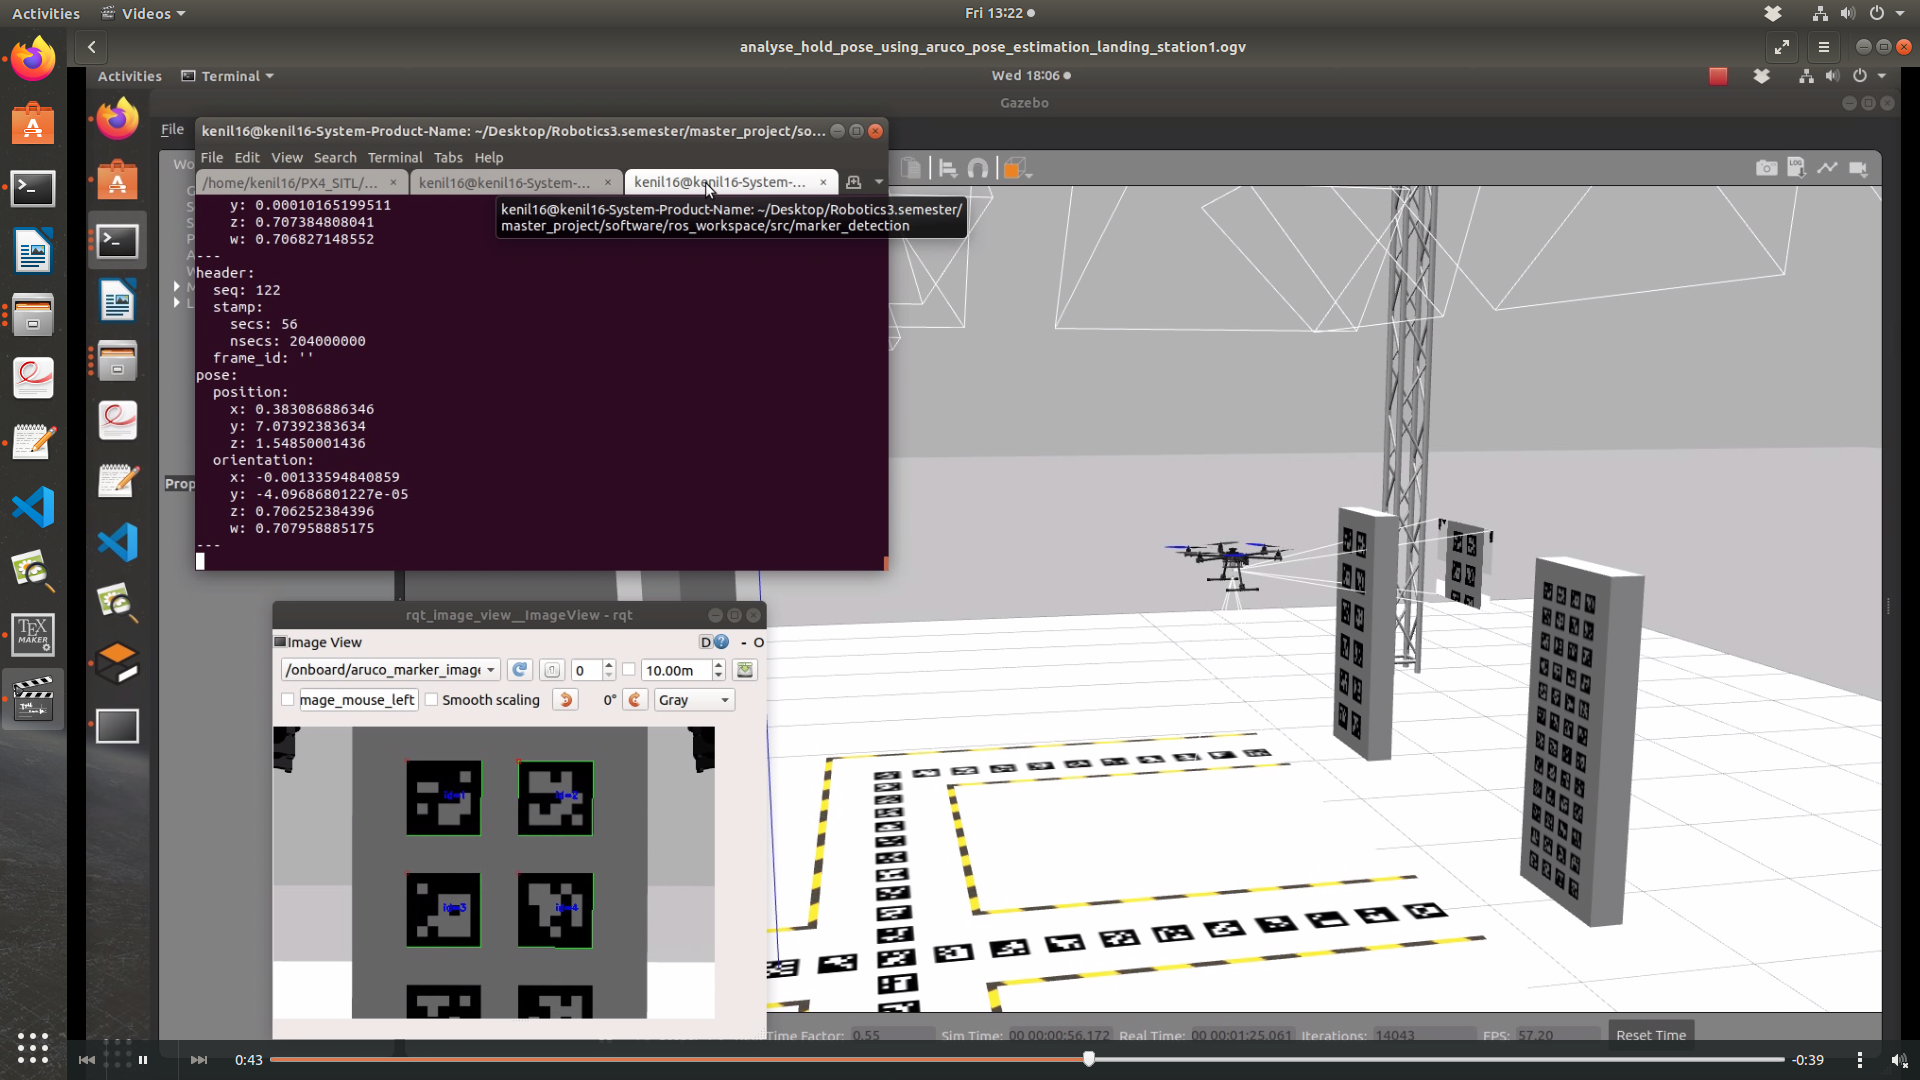
\includegraphics[width=\textwidth]{../Figures/hold_pose_using_aruco_pose_estimation/aruco_board_three.png}
        \caption{}
        \label{fig:hold_pose_aruco_board_three}
    \end{subfigure}
     \hspace{0.2em}
    \begin{subfigure}[t]{.30\textwidth}
        \centering
        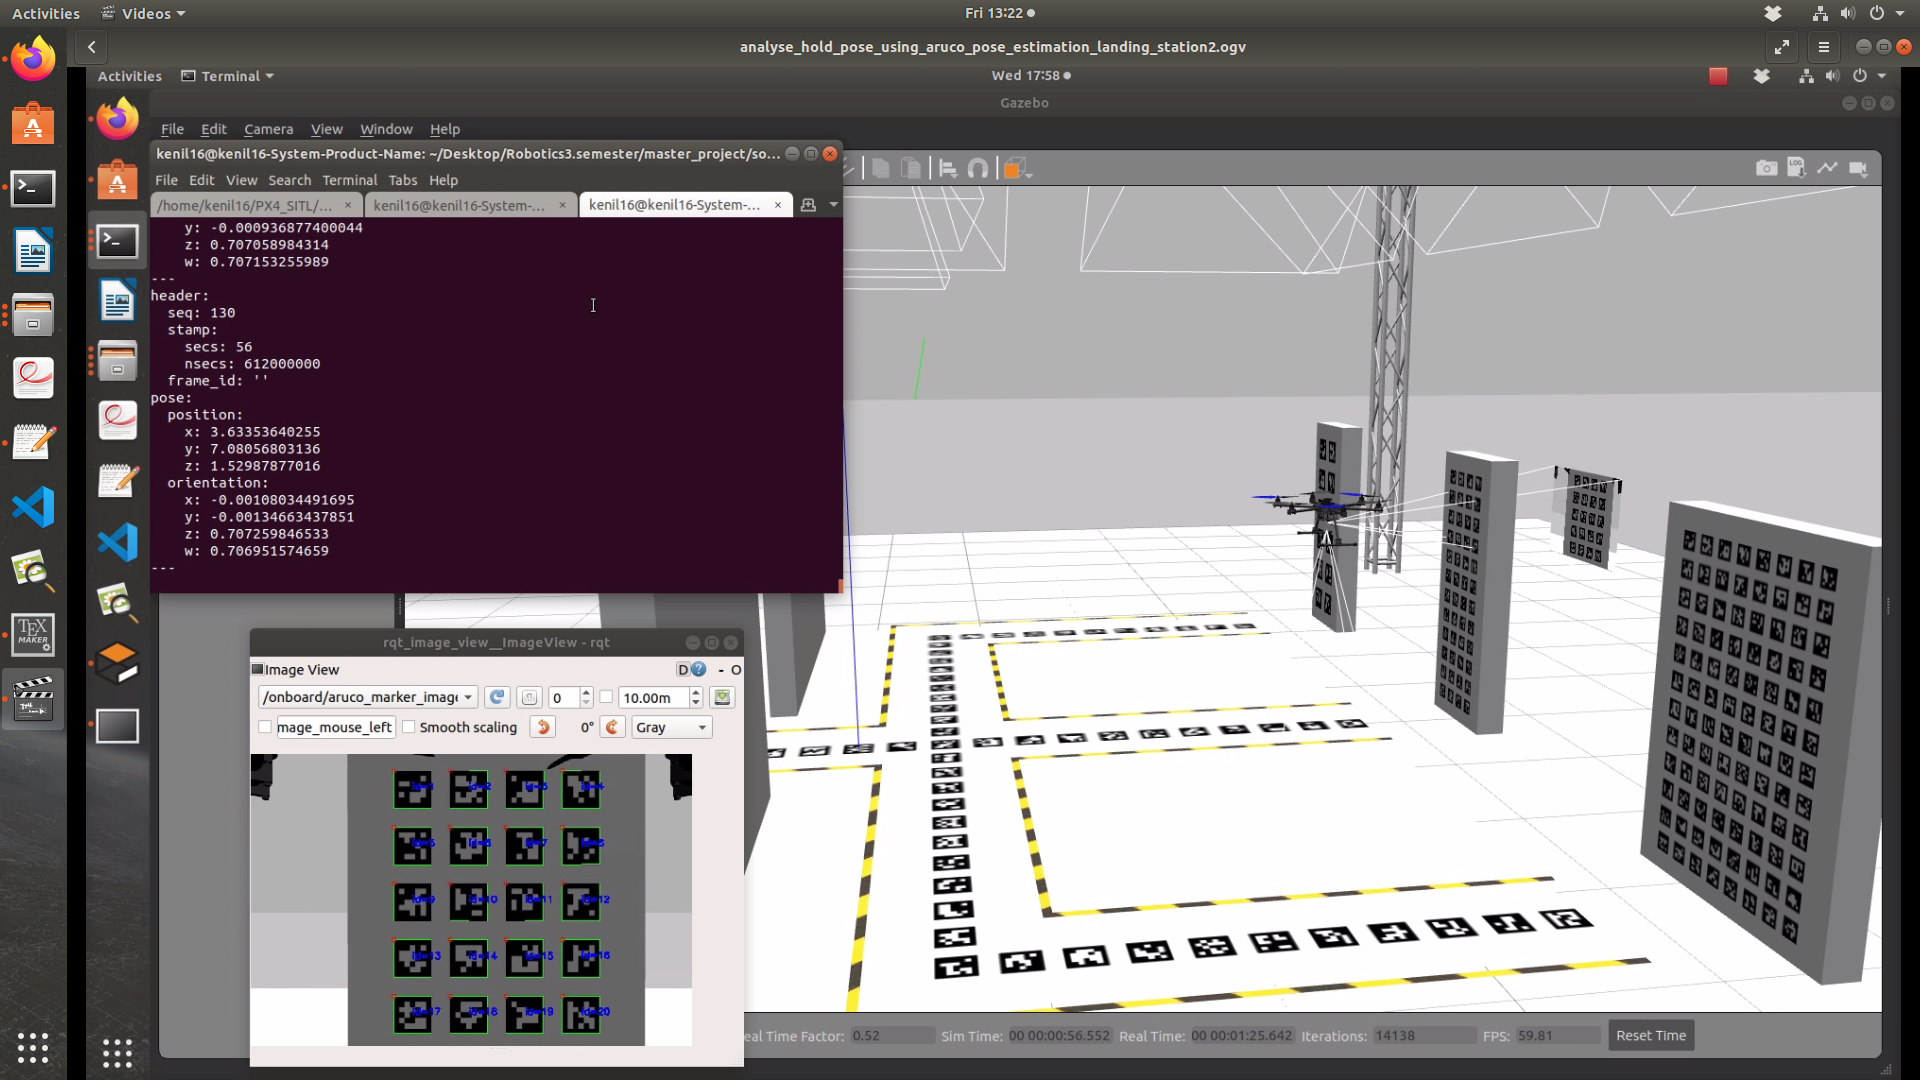
\includegraphics[width=\textwidth]{../Figures/hold_pose_using_aruco_pose_estimation/aruco_board_four.png}
        \caption{}
        \label{fig:hold_pose_aruco_board_four}
    \end{subfigure}
     \hspace{0.2em}
    \begin{subfigure}[t]{.30\textwidth}
        \centering
        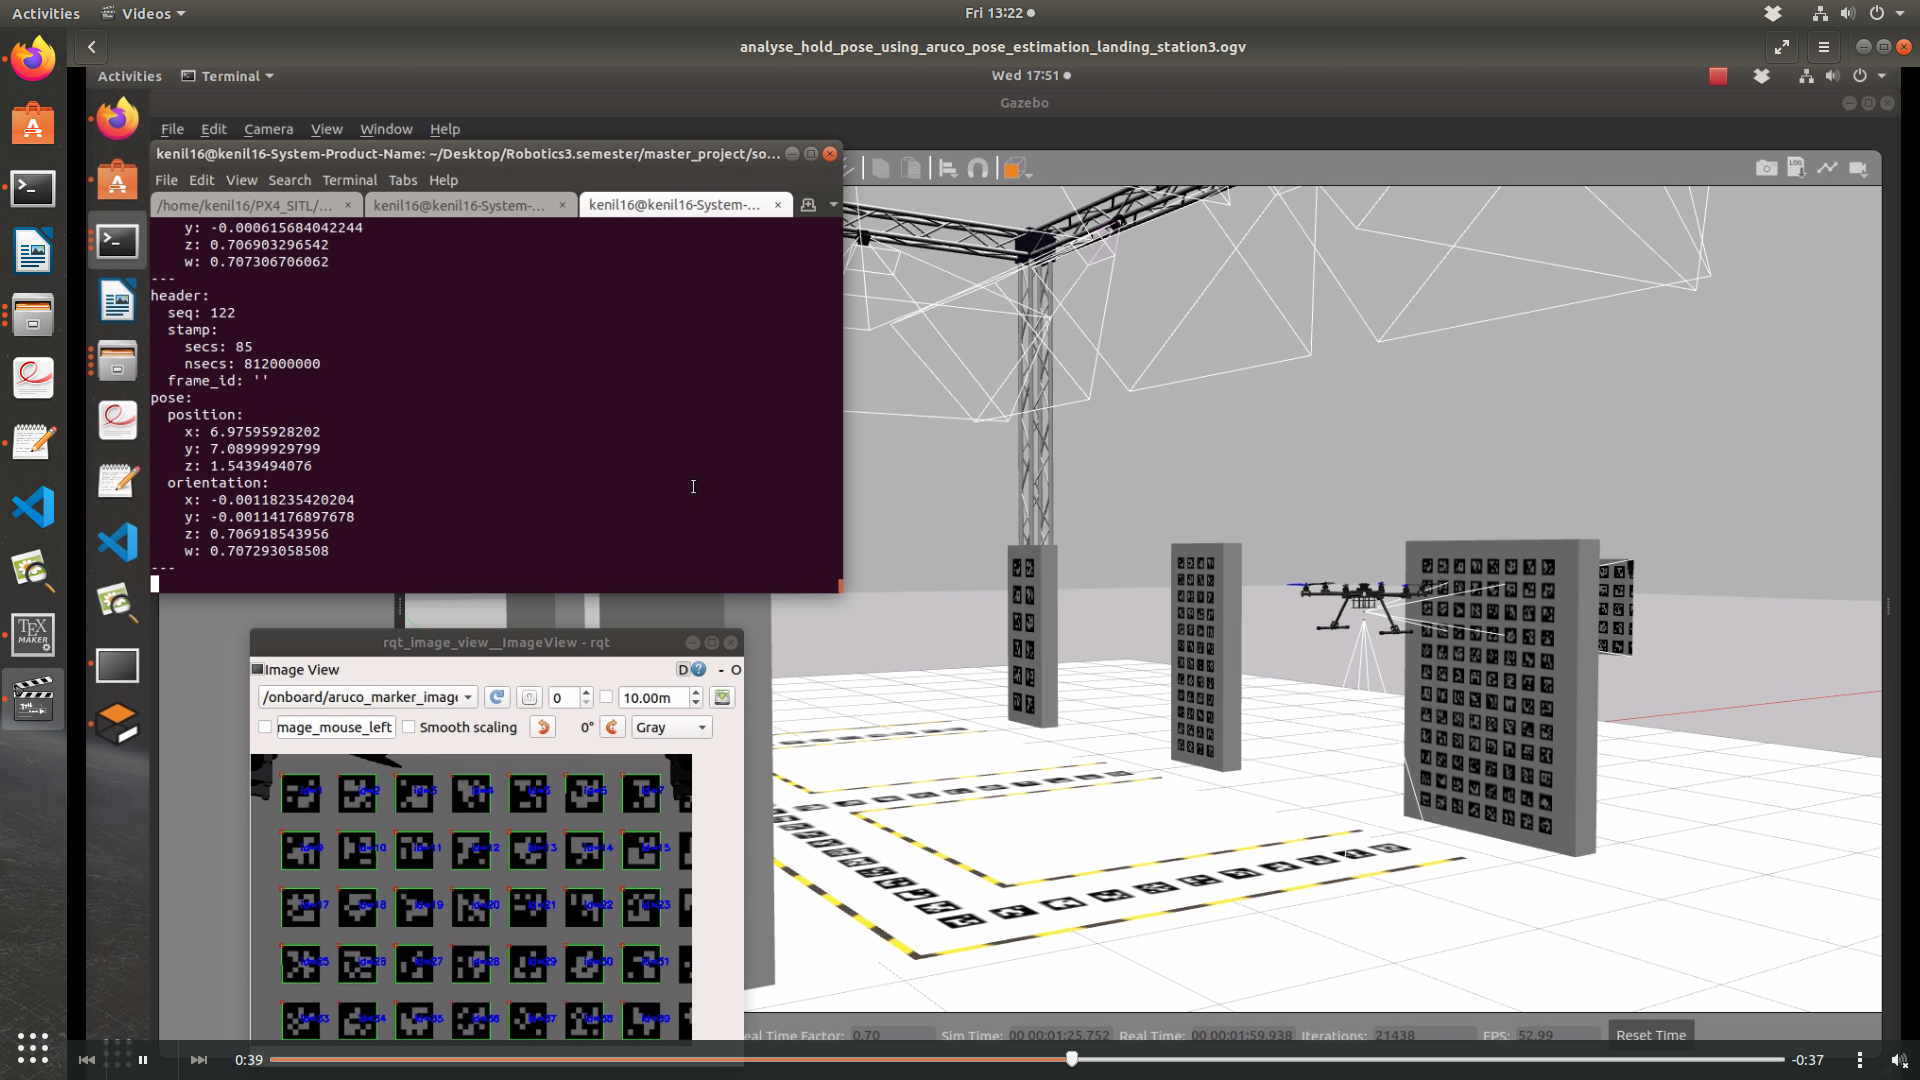
\includegraphics[width=\textwidth]{../Figures/hold_pose_using_aruco_pose_estimation/aruco_board_five.png}
        \caption{}
        \label{fig:hold_pose_aruco_board_five}
    \end{subfigure}
    \hspace{0.2em}
        \begin{subfigure}[t]{.30\textwidth}
        \centering
        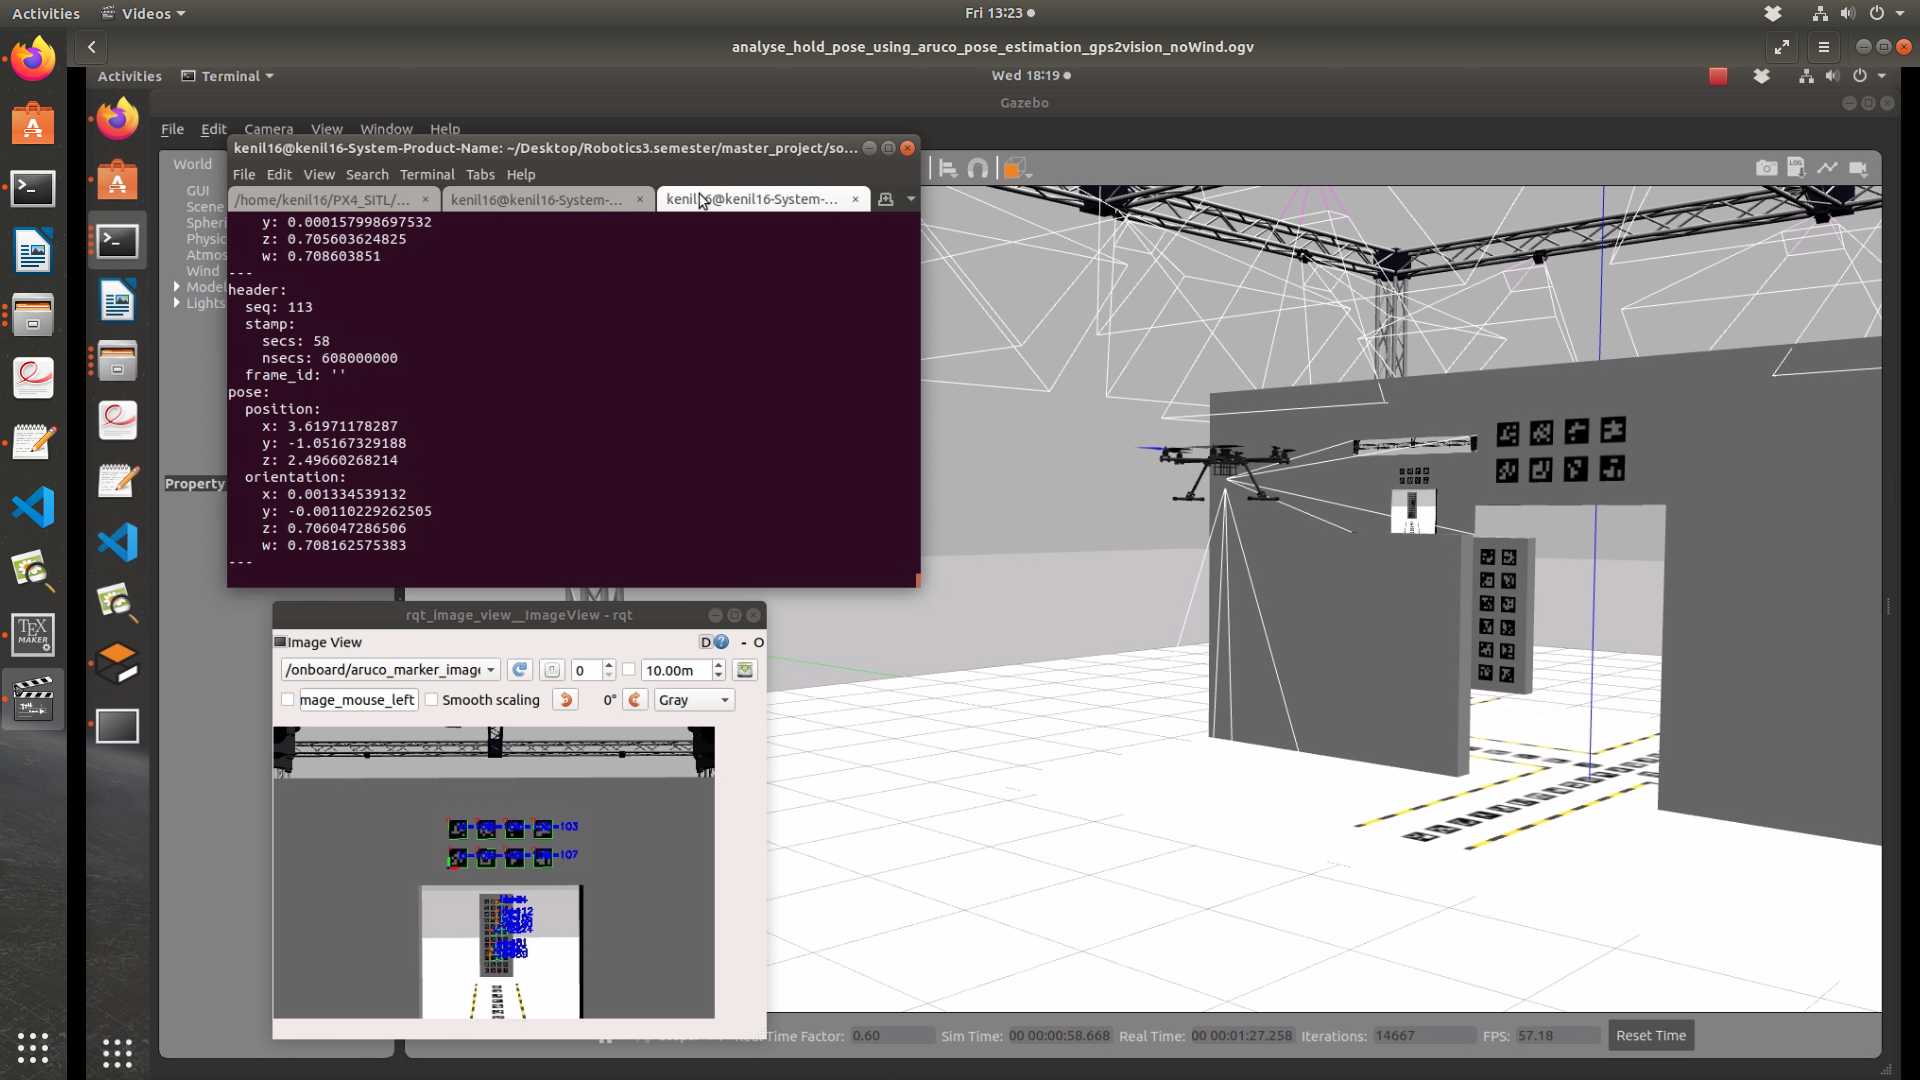
\includegraphics[width=\textwidth]{../Figures/hold_pose_using_aruco_pose_estimation/aruco_board_one_noWind.png}
        \caption{}
        \label{fig:hold_pose_aruco_board_one_noWind}
    \end{subfigure}
        \begin{subfigure}[t]{.30\textwidth}
        \centering
        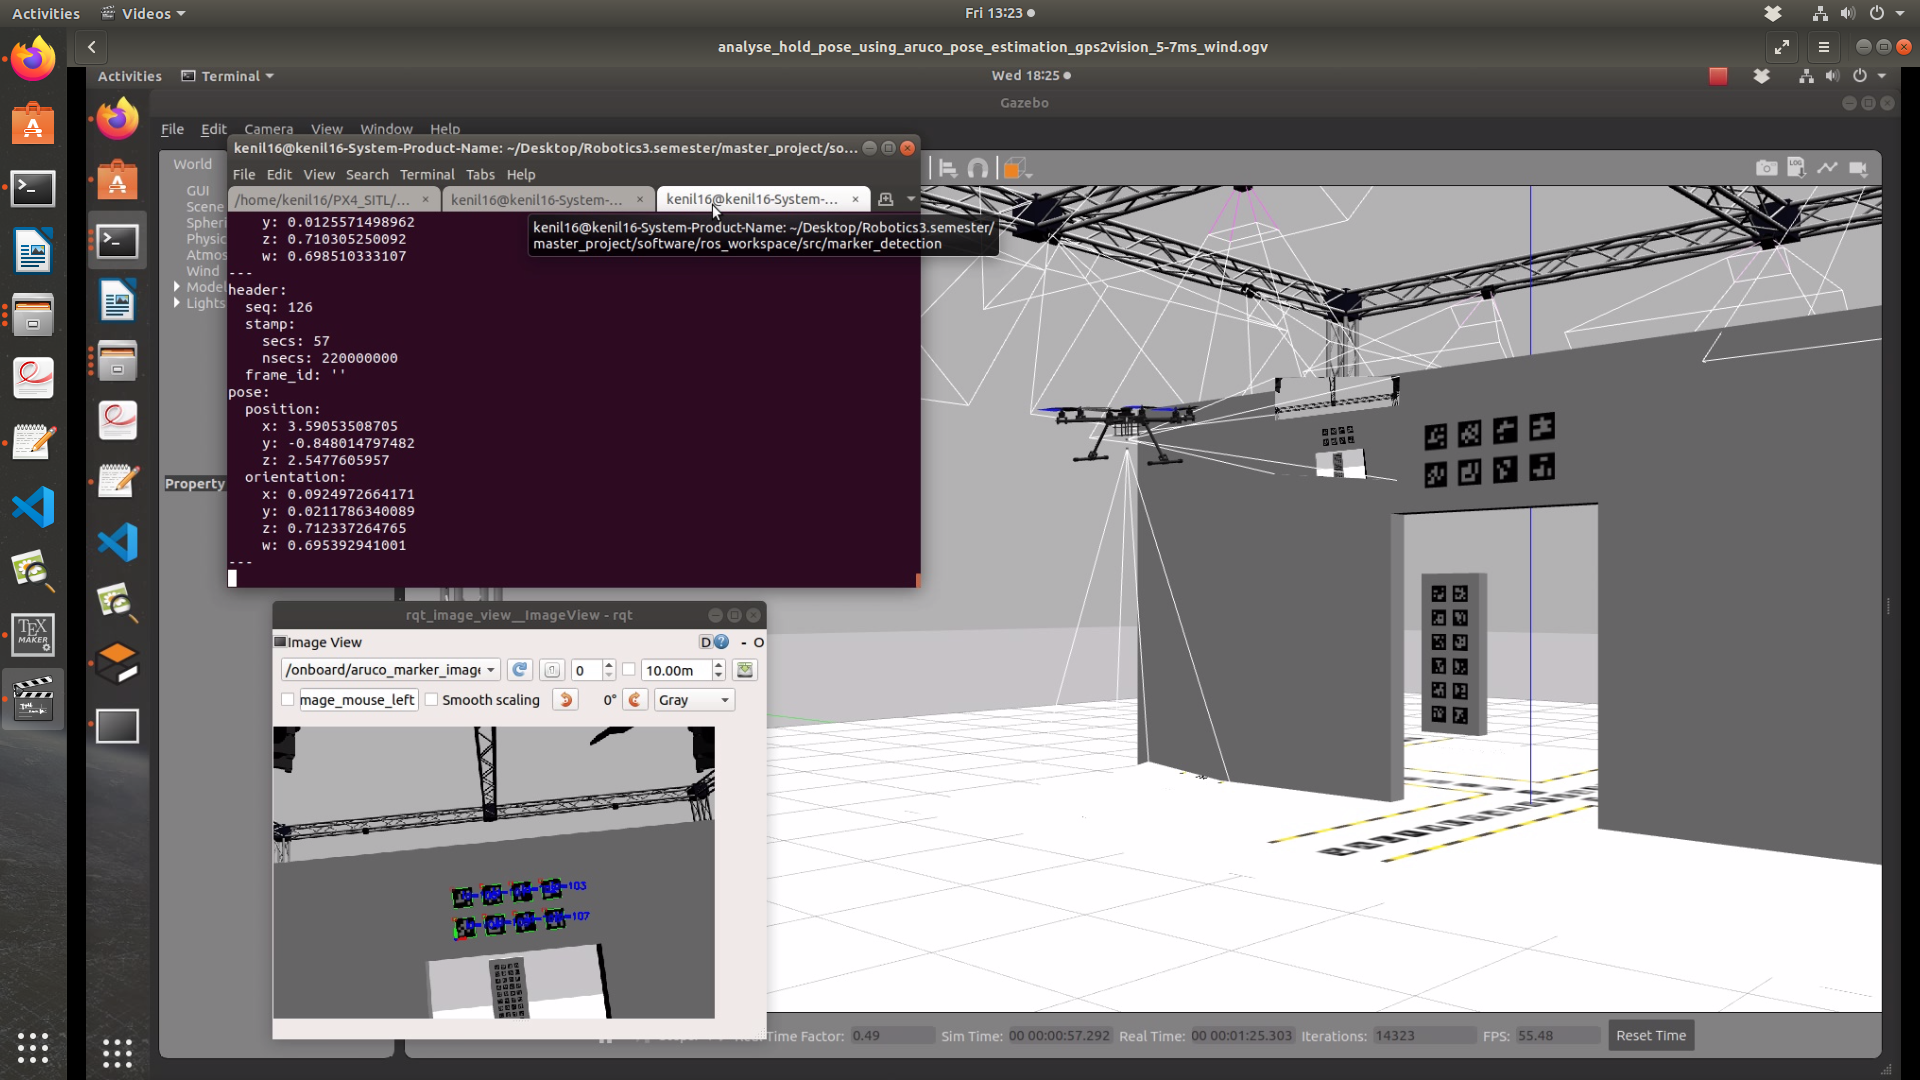
\includegraphics[width=\textwidth]{../Figures/hold_pose_using_aruco_pose_estimation/aruco_board_one_5-7ms_wind.png}
        \caption{}
        \label{fig:hold_pose_aruco_board_one_5-7ms_wind}
    \end{subfigure}
    \caption{Illustrations of the different configurations for the tests. The ArUco landing boards are used in Figures \ref{fig:hold_pose_aruco_board_three}, \ref{fig:hold_pose_aruco_board_four} and \ref{fig:hold_pose_aruco_board_five} for landing stations one, two and three respectively. The GPS2Vision board is used in \ref{fig:hold_pose_aruco_board_one_noWind} and \ref{fig:hold_pose_aruco_board_one_5-7ms_wind} without and with simulated wind. Videos of the tests can be seen on Github using \href{https://github.com/Kenil16/master_project/tree/master/test_videos/analyse_hold_pose_using_aruco_pose_estimation_landing_station1}{Landing station one}, \href{https://github.com/Kenil16/master_project/tree/master/test_videos/analyse_hold_pose_using_aruco_pose_estimation_landing_station2}{Landing station two}, \href{https://github.com/Kenil16/master_project/tree/master/test_videos/analyse_hold_pose_using_aruco_pose_estimation_landing_station3}{Landing station three}, \href{https://github.com/Kenil16/master_project/tree/master/test_videos/analyse_hold_pose_using_aruco_pose_estimation_gps2vision_noWind}{GPS2Vision board} and  \href{https://github.com/Kenil16/master_project/tree/master/test_videos/analyse_hold_pose_using_aruco_pose_estimation_gps2vision_5-7ms_wind}{GPS2Vision board with 5-7 $\frac{m}{s}$ wind}}
    \label{fig:hold_pose_aruco_boards}
\end{figure}

To analyses how the ArUco pose estimations effects the algorithms for pose control, the UAV was set to hold its pose for 30 seconds in a number of different configurations as seen in Figure \ref{fig:hold_pose_aruco_boards}. 


In Figures \ref{fig:hold_pose_aruco_board_three}, \ref{fig:hold_pose_aruco_board_four} and \ref{fig:hold_pose_aruco_board_five}, the ArUco landing boards are used where the UAV are set to keep its pose one meter in front of the board with an altitude of 1.5 meters. This is done to insure that most of the markers in the board can be seen in the image without been too close to the board to cause damage to the UAV. In Figures \ref{fig:hold_pose_aruco_board_one_noWind} and \ref{fig:hold_pose_aruco_board_one_5-7ms_wind}, the GPS2Vision board is used without and with simulated wind. Here the UAV are set to keep and altitude of 2.5 meters approximately 4 meters in front of the board.

This distance in front of the GPS2Vision board is chosen on the basis of the results in Section \ref{sec:GPS2Vision_pose_estimation} and \ref{sec:rolling_average_aruco_pose_estimation} which was found to be a safe transition area when going from using GPS to vision based navigation.   

\begin{table}[H]
    \centering
    \addtolength{\leftskip} {-2cm}
    \addtolength{\rightskip}{-2cm}
        \caption{Statistics of the results of holding the pose using the GPS2Vision boards. It may be noticed that adding wind to the simulation, hence giving the UAV an angle in roll and pitch, does not seem no effect the pose estimation error significantly. Only the target setpoints are effected}
        \pgfplotstabletypeset[normal,
                columns/eg/.style={
                column name={Runs},
                dec sep align
        }
        ]{ %
        Estimation error & eg & Wind & Mean position & STD position & Mean angle & STD angle\\
        \topmidheader{8}{\textbf{Test 1}}
ArUco pose GPV2Vision board & 10      & No & $1.43cm$ & $1.10cm$ & $0.18^{\circ}$ & $0.13^{\circ}$\\
Setpoint         & 10      & No & $3.12cm $ & $2.58cm$ & $0.28^{\circ}$ & $0.22^{\circ}$\\
		\midheader{8}{\textbf{Test 2}}
ArUco pose GPV2Vision board & 10      & 5-7 $\frac{m}{s}$ & $1.47cm $ & $0.95cm$ & $0.49^{\circ}$ & $0.31^{\circ}$\\
Setpoint         & 10      & 5-7 $\frac{m}{s}$ & $4.04cm $ & $3.35cm$ & $4.45^{\circ}$ & $1.49^{\circ}$\\
 }
 \label{tab:hold_pose_using_gps2vision_board}
\end{table}

\begin{table}[H]
    \centering
    \addtolength{\leftskip} {-2cm}
    \addtolength{\rightskip}{-2cm}
        \caption{Statistics of the results of holding the pose using the ArUco landing boards. It may be noticed that as more ArUco markers are present in the image, the lesser is the pose estimation error. However, no significant decrease in the pose estimation error is seen between using landing board one and three even though the entire image is filled with ArUco markers as seen in Figure \ref{fig:hold_pose_aruco_board_five}}
        \pgfplotstabletypeset[normal,
                columns/eg/.style={
                column name={Runs},
                dec sep align
        }
        ]{ %
        Estimation error & eg & Wind & Mean position & STD position & Mean angle & STD angle\\
        \topmidheader{8}{\textbf{Test 3}}
ArUco pose landing board one       & 10      & No & $0.12cm $ & $0.23cm$ & $0.03^{\circ}$ & $0.05^{\circ}$\\
Setpoint         & 10      & No & $2.93cm$ & $2.90cm$ & $0.12^{\circ}$ & $0.12^{\circ}$\\
		\midheader{8}{\textbf{Test 4}}
ArUco pose landing board two       & 10      & No & $0.11cm $ & $0.21cm$ & $0.02^{\circ}$ & $0.01^{\circ}$\\
Setpoint         & 10      & No & $2.92cm$ & $2.89cm$ & $0.11^{\circ}$ & $0.09^{\circ}$\\
		\midheader{8}{\textbf{Test 5}}
ArUco pose landing board three       & 10      & No & $0.09cm $ & $0.20cm$ &
$0.02^{\circ}$ & $0.01^{\circ}$\\
Setpoint         & 10      & No & $2.89cm$ & $2.85cm$ & $0.11^{\circ}$ & $0.09^{\circ}$\\
 }
 \label{tab:hold_pose_using_landing_station_boards}
\end{table}


\begin{figure}[H]
    \centering
    \begin{subfigure}[t]{.30\textwidth}
        \centering
        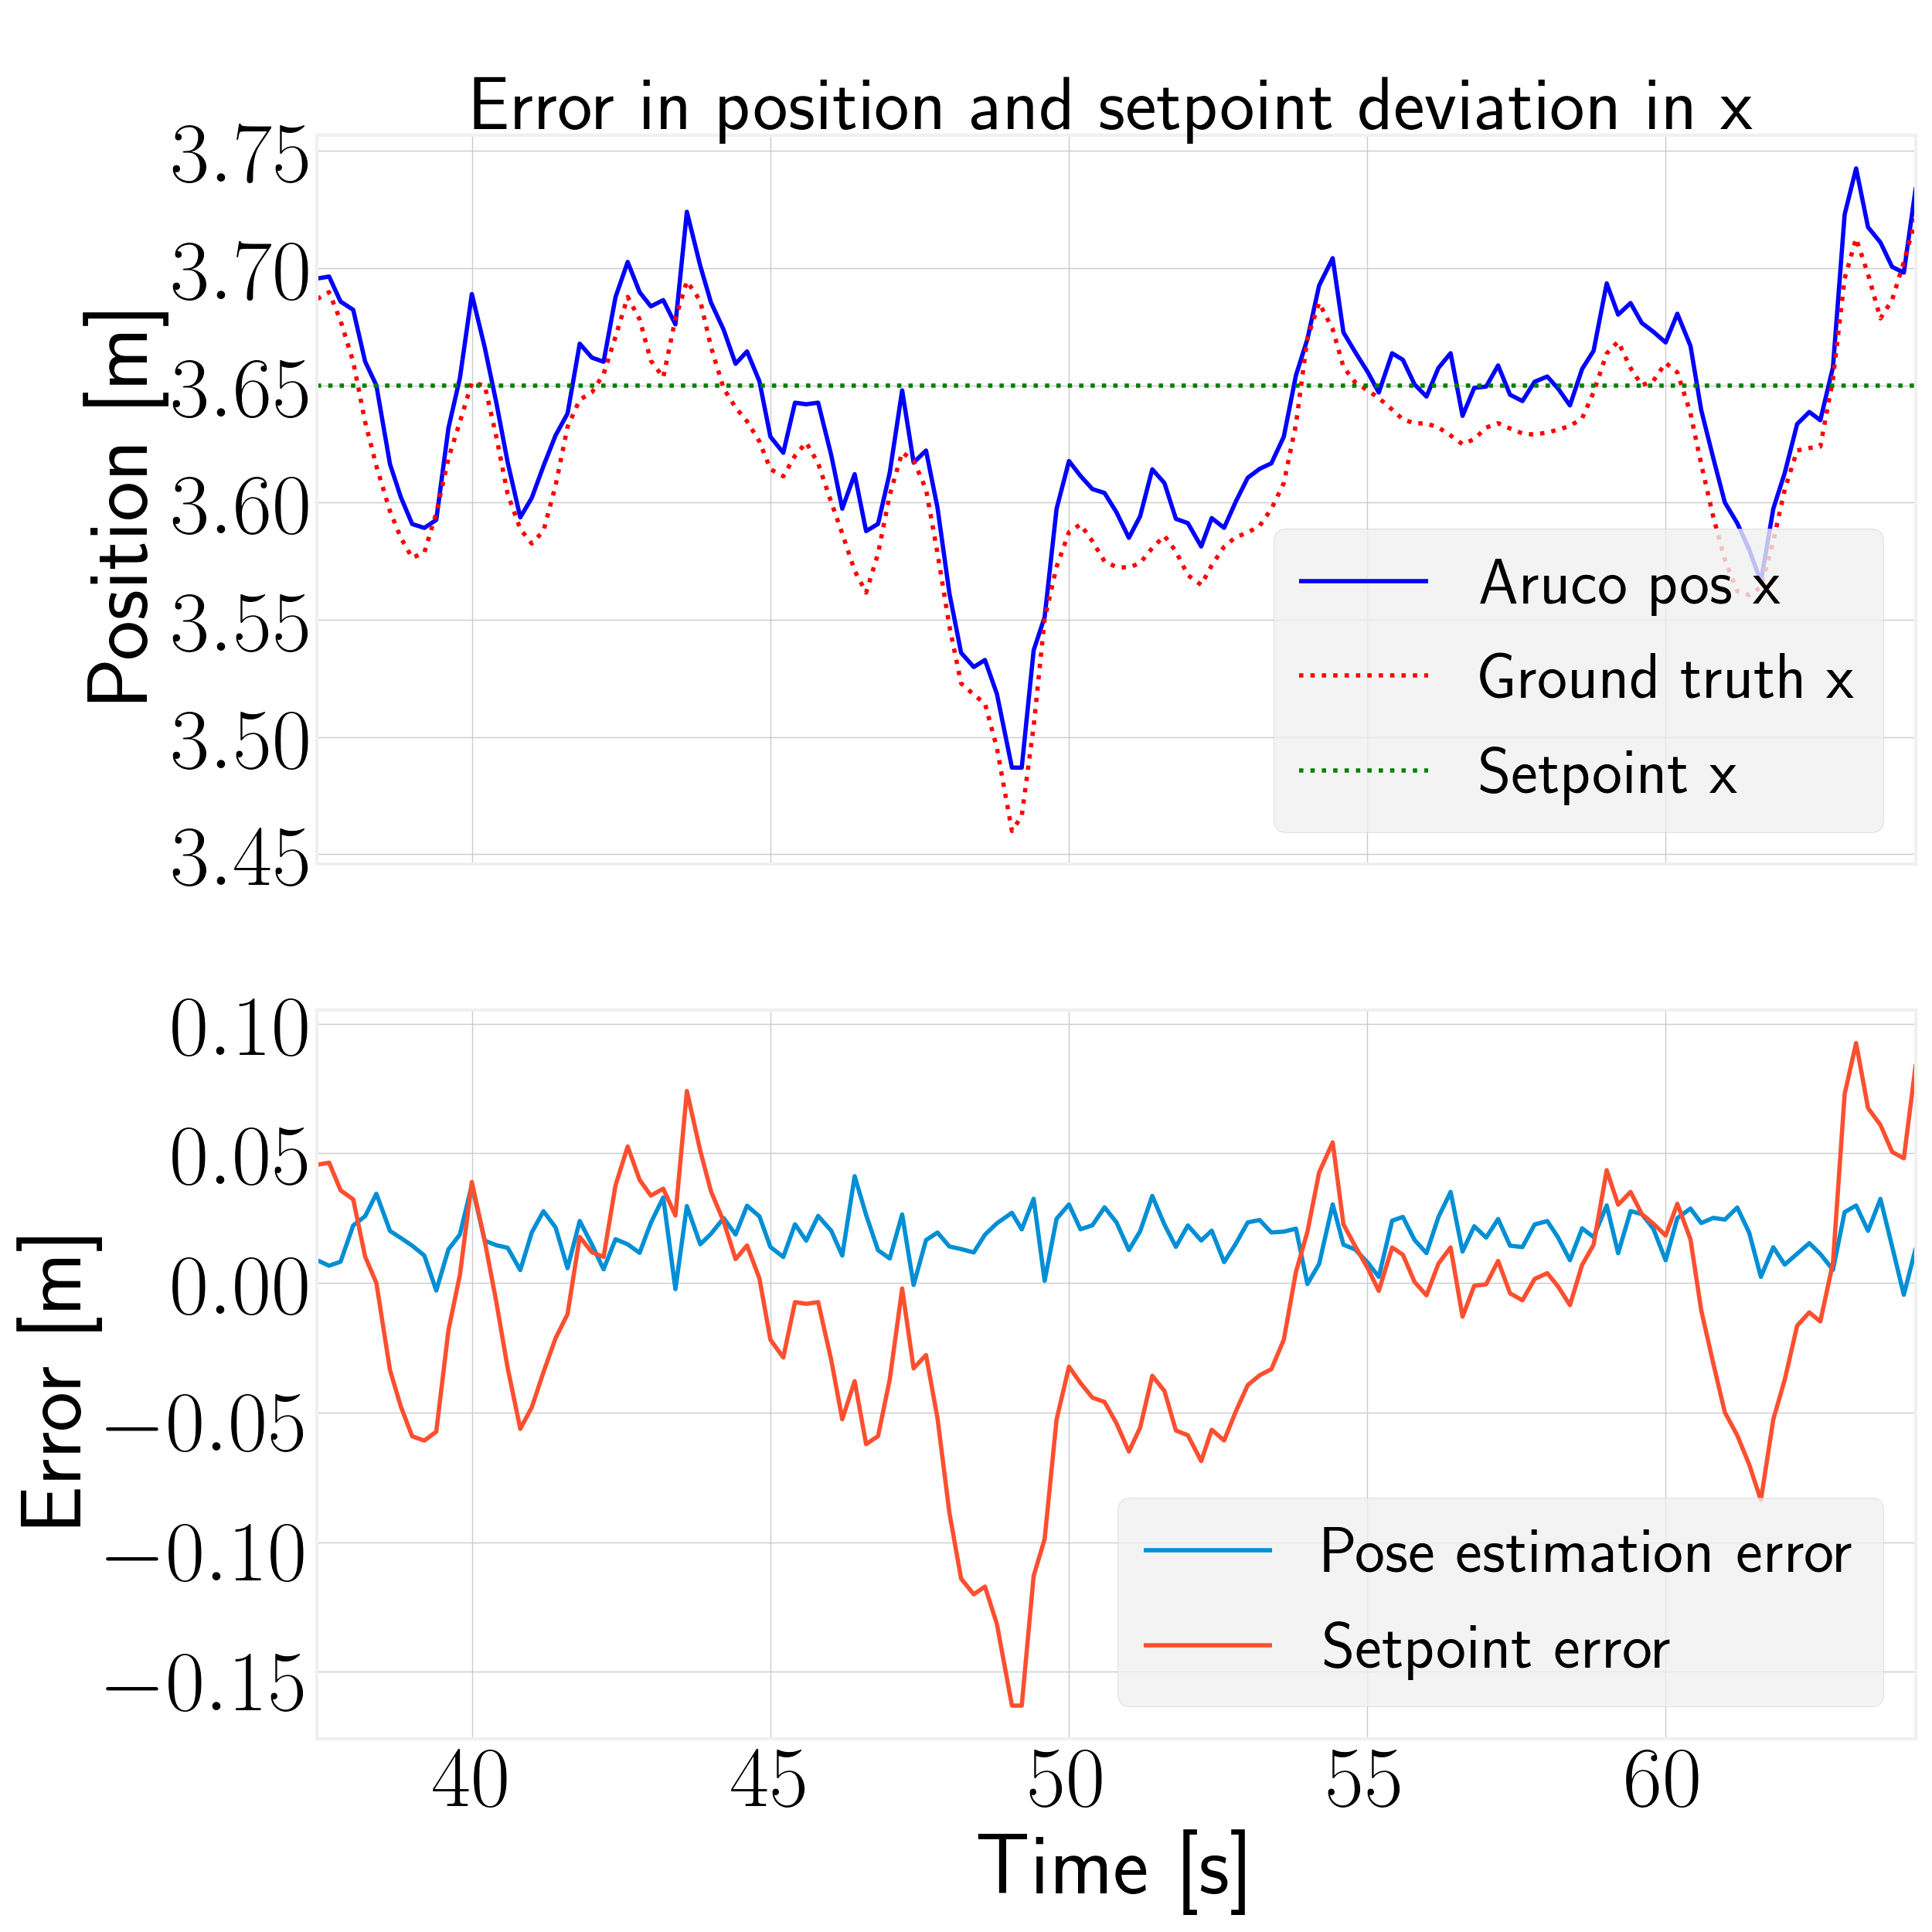
\includegraphics[width=\textwidth]{../Figures/hold_pose_using_aruco_pose_estimation/pose_error_x_test2.png}
        \caption{}
        \label{fig:hold_pose_estimation_test2_x}
    \end{subfigure}
     \hspace{0.2em}
    \begin{subfigure}[t]{.30\textwidth}
        \centering
        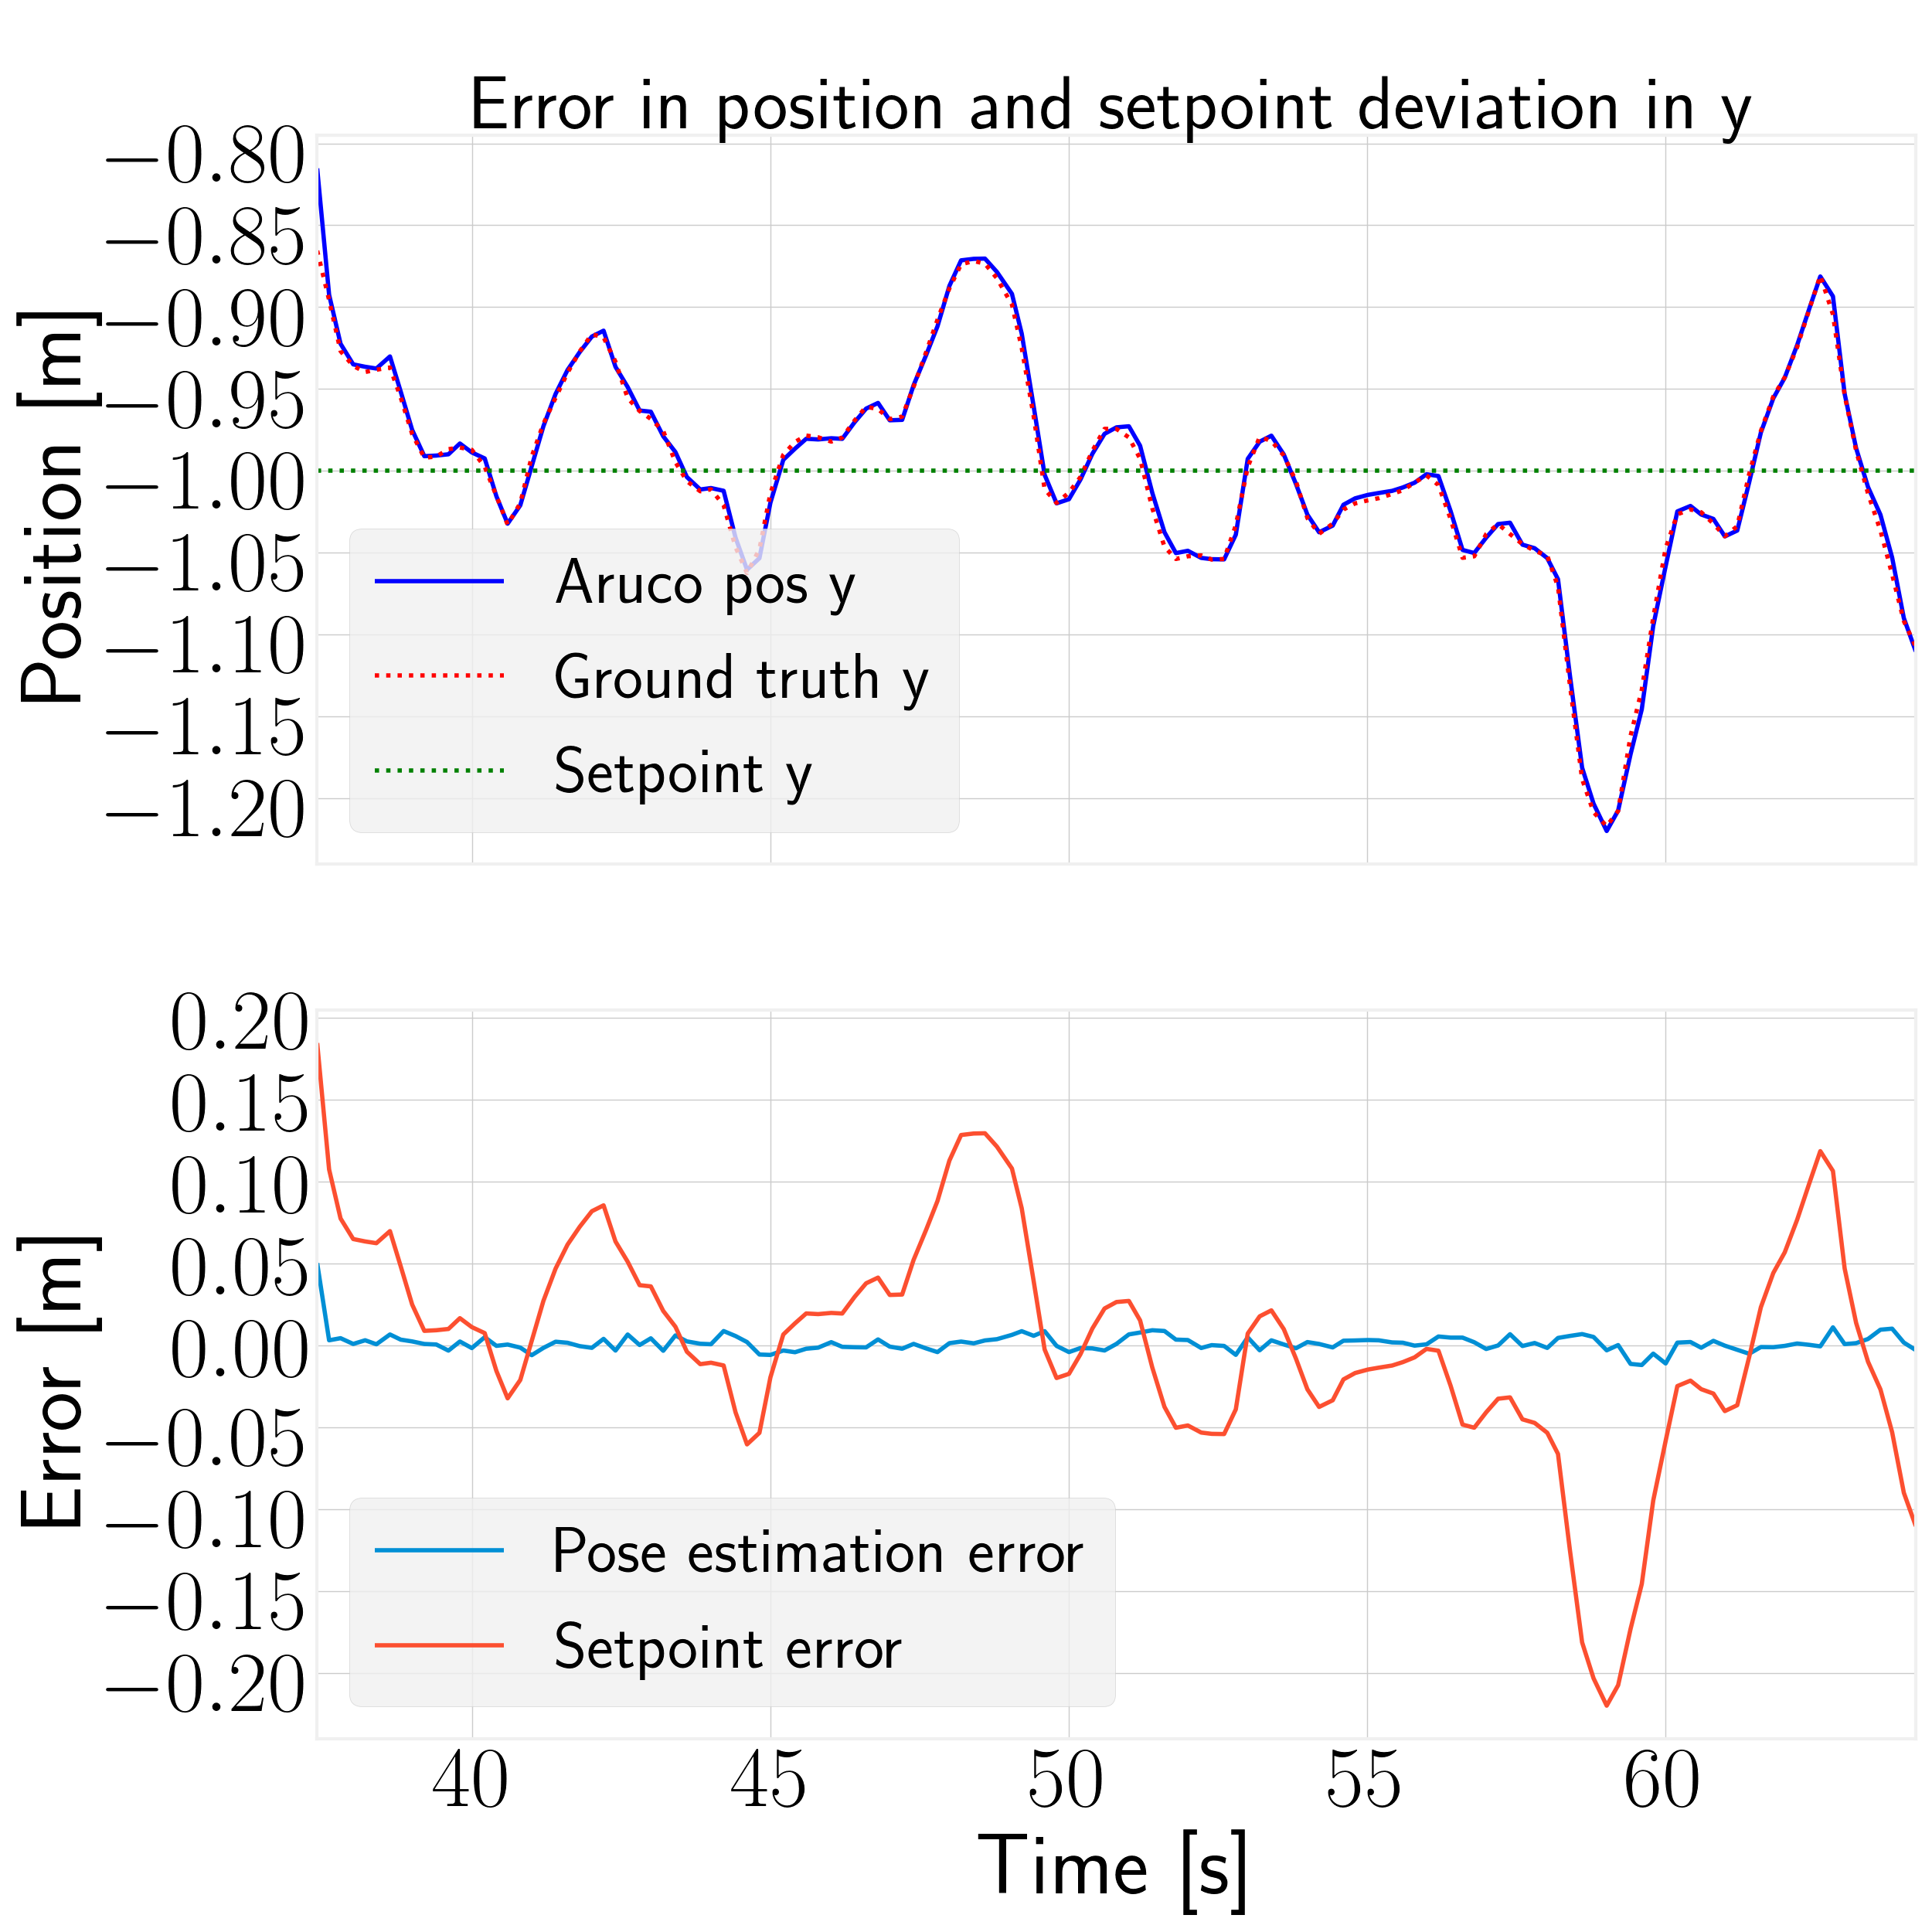
\includegraphics[width=\textwidth]{../Figures//hold_pose_using_aruco_pose_estimation/pose_error_y_test2.png}
        \caption{}
        \label{fig:hold_pose_estimation_test2_y}
    \end{subfigure}
     \hspace{0.2em}
    \begin{subfigure}[t]{.30\textwidth}
        \centering
        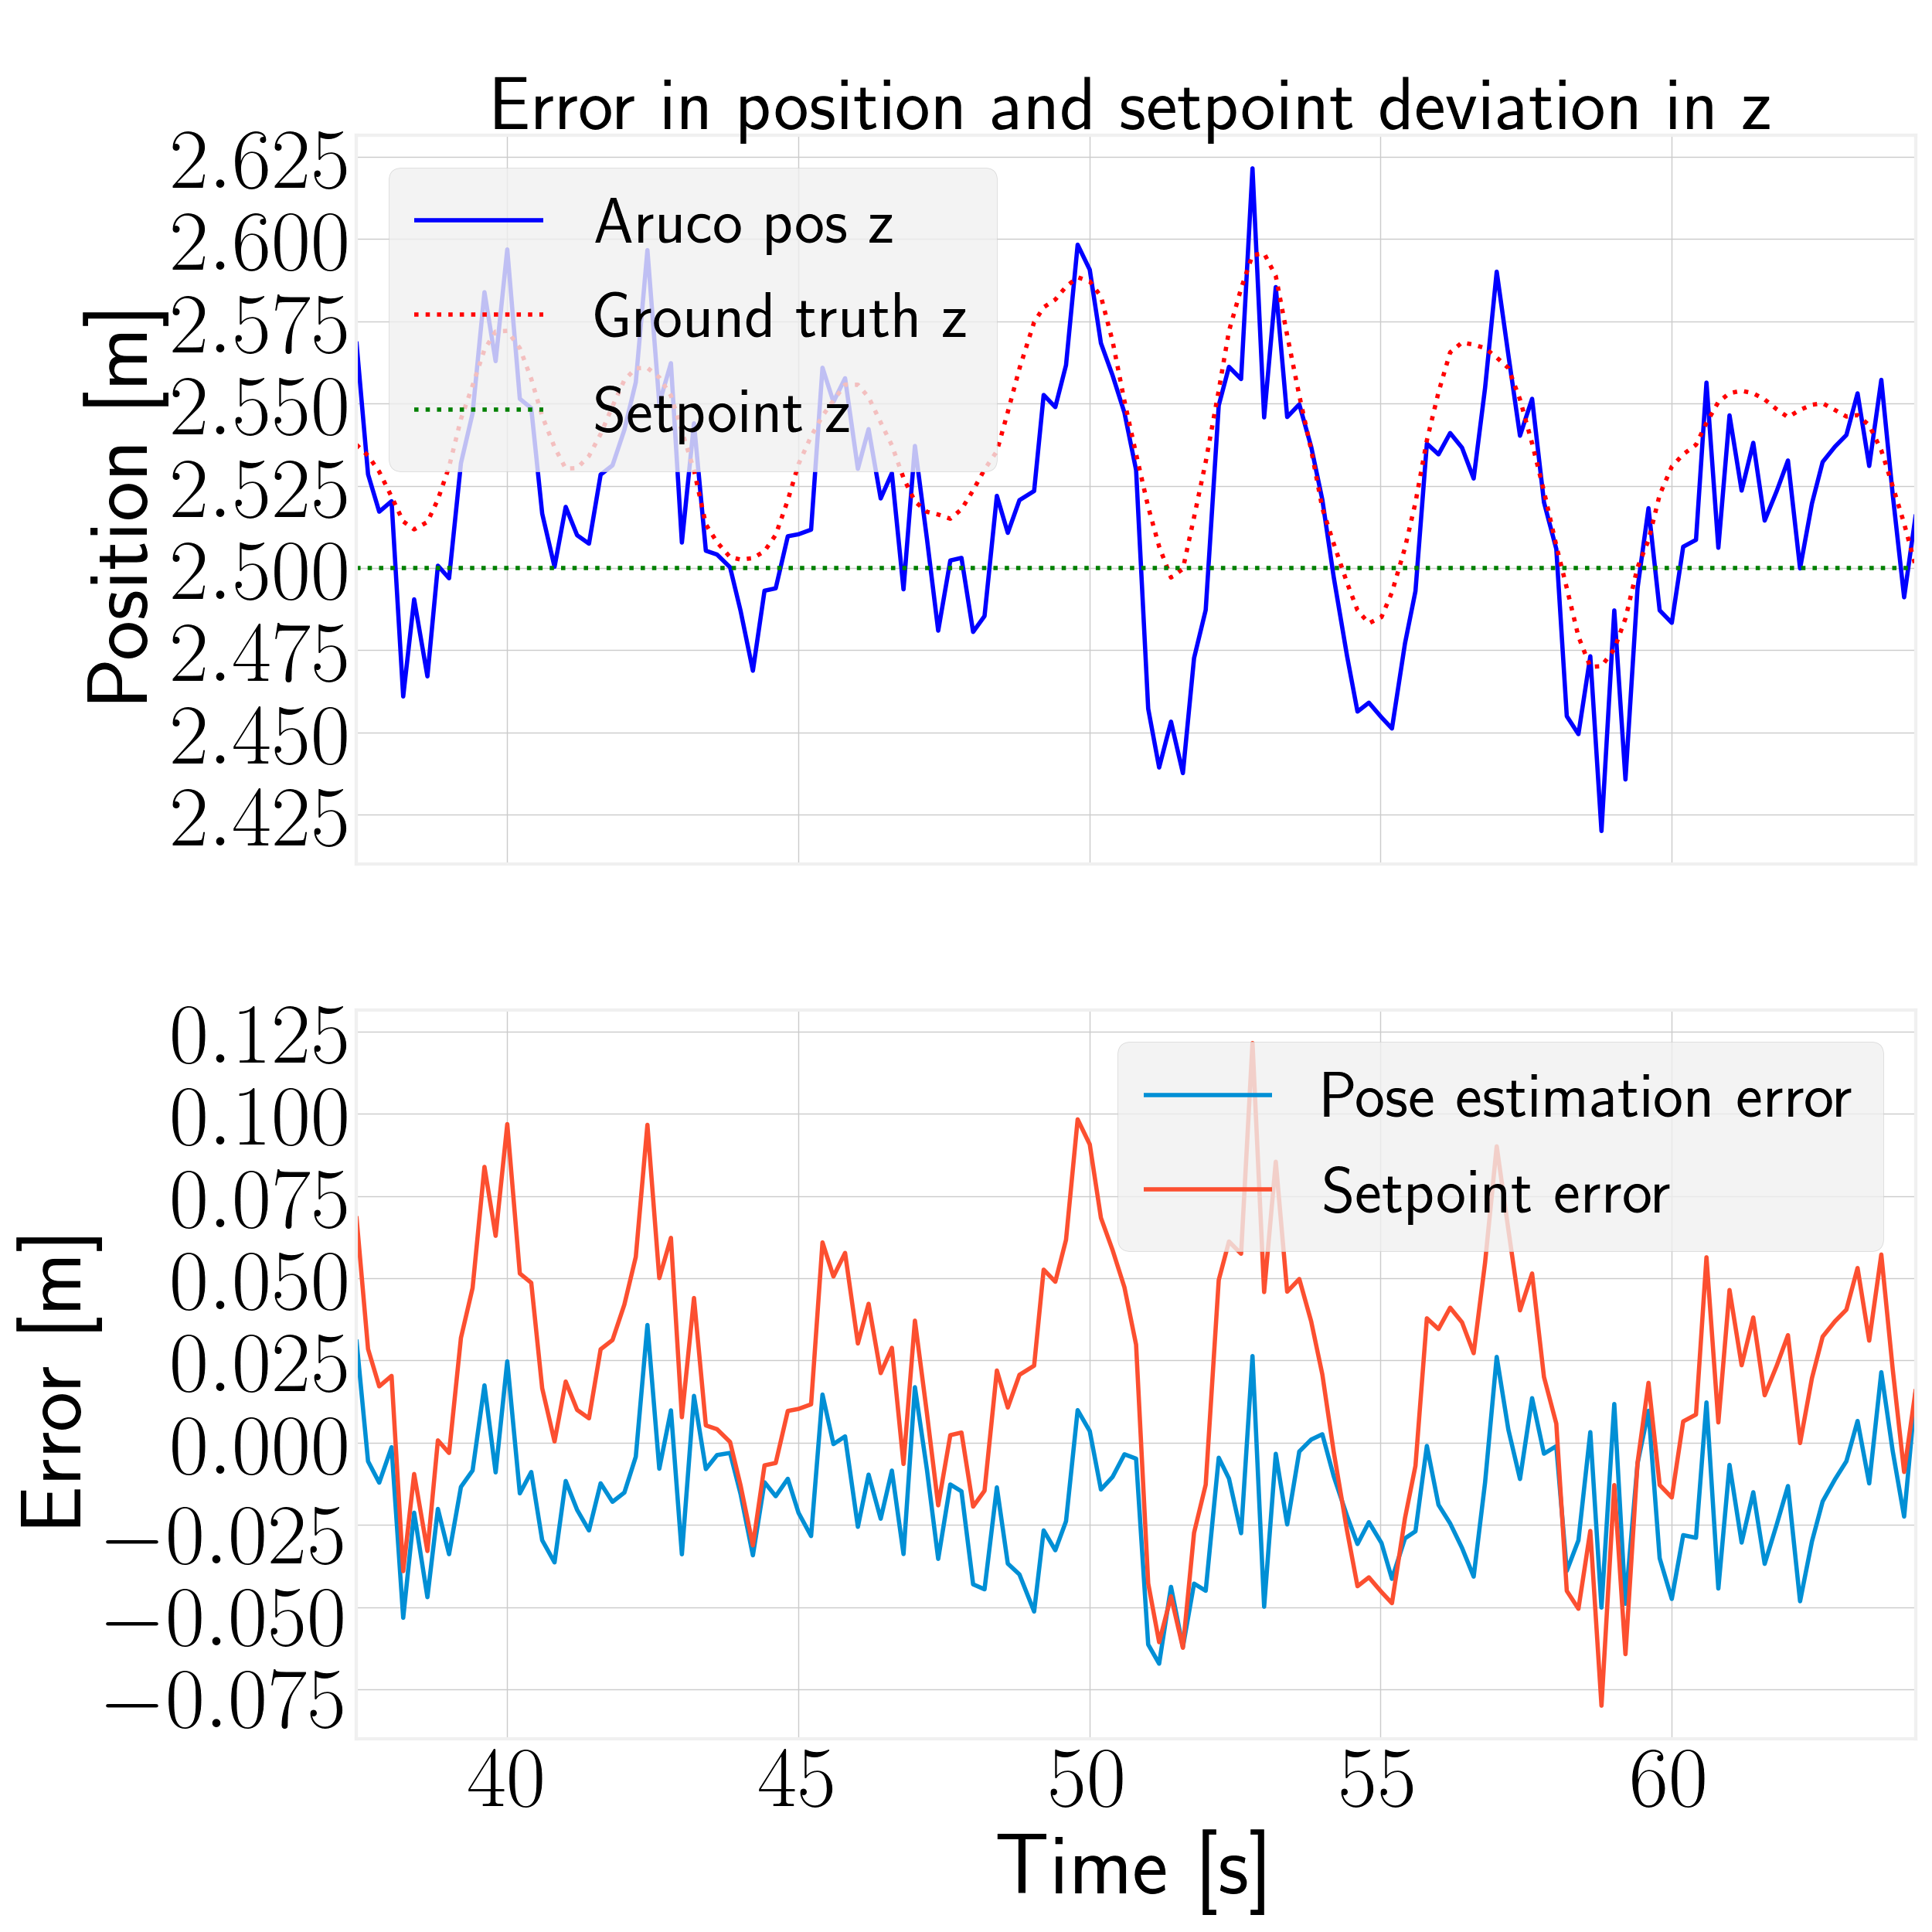
\includegraphics[width=\textwidth]{../Figures/hold_pose_using_aruco_pose_estimation/pose_error_z_test2.png}
        \caption{}
        \label{fig:hold_pose_estimation_test2_z}
    \end{subfigure}
    \caption{Illustration of the pose estimation and setpoint error using configuration in Figure \ref{fig:hold_pose_aruco_board_one_5-7ms_wind}. It may be noticed that the pose estimation errors in x and y are in the orders of centimeters with a bit increase in error in z}
    \label{fig:hold_pose_estimation_test2_error_pos}
\end{figure}

\begin{figure}[H]
    \centering
    \begin{subfigure}[t]{.30\textwidth}
        \centering
        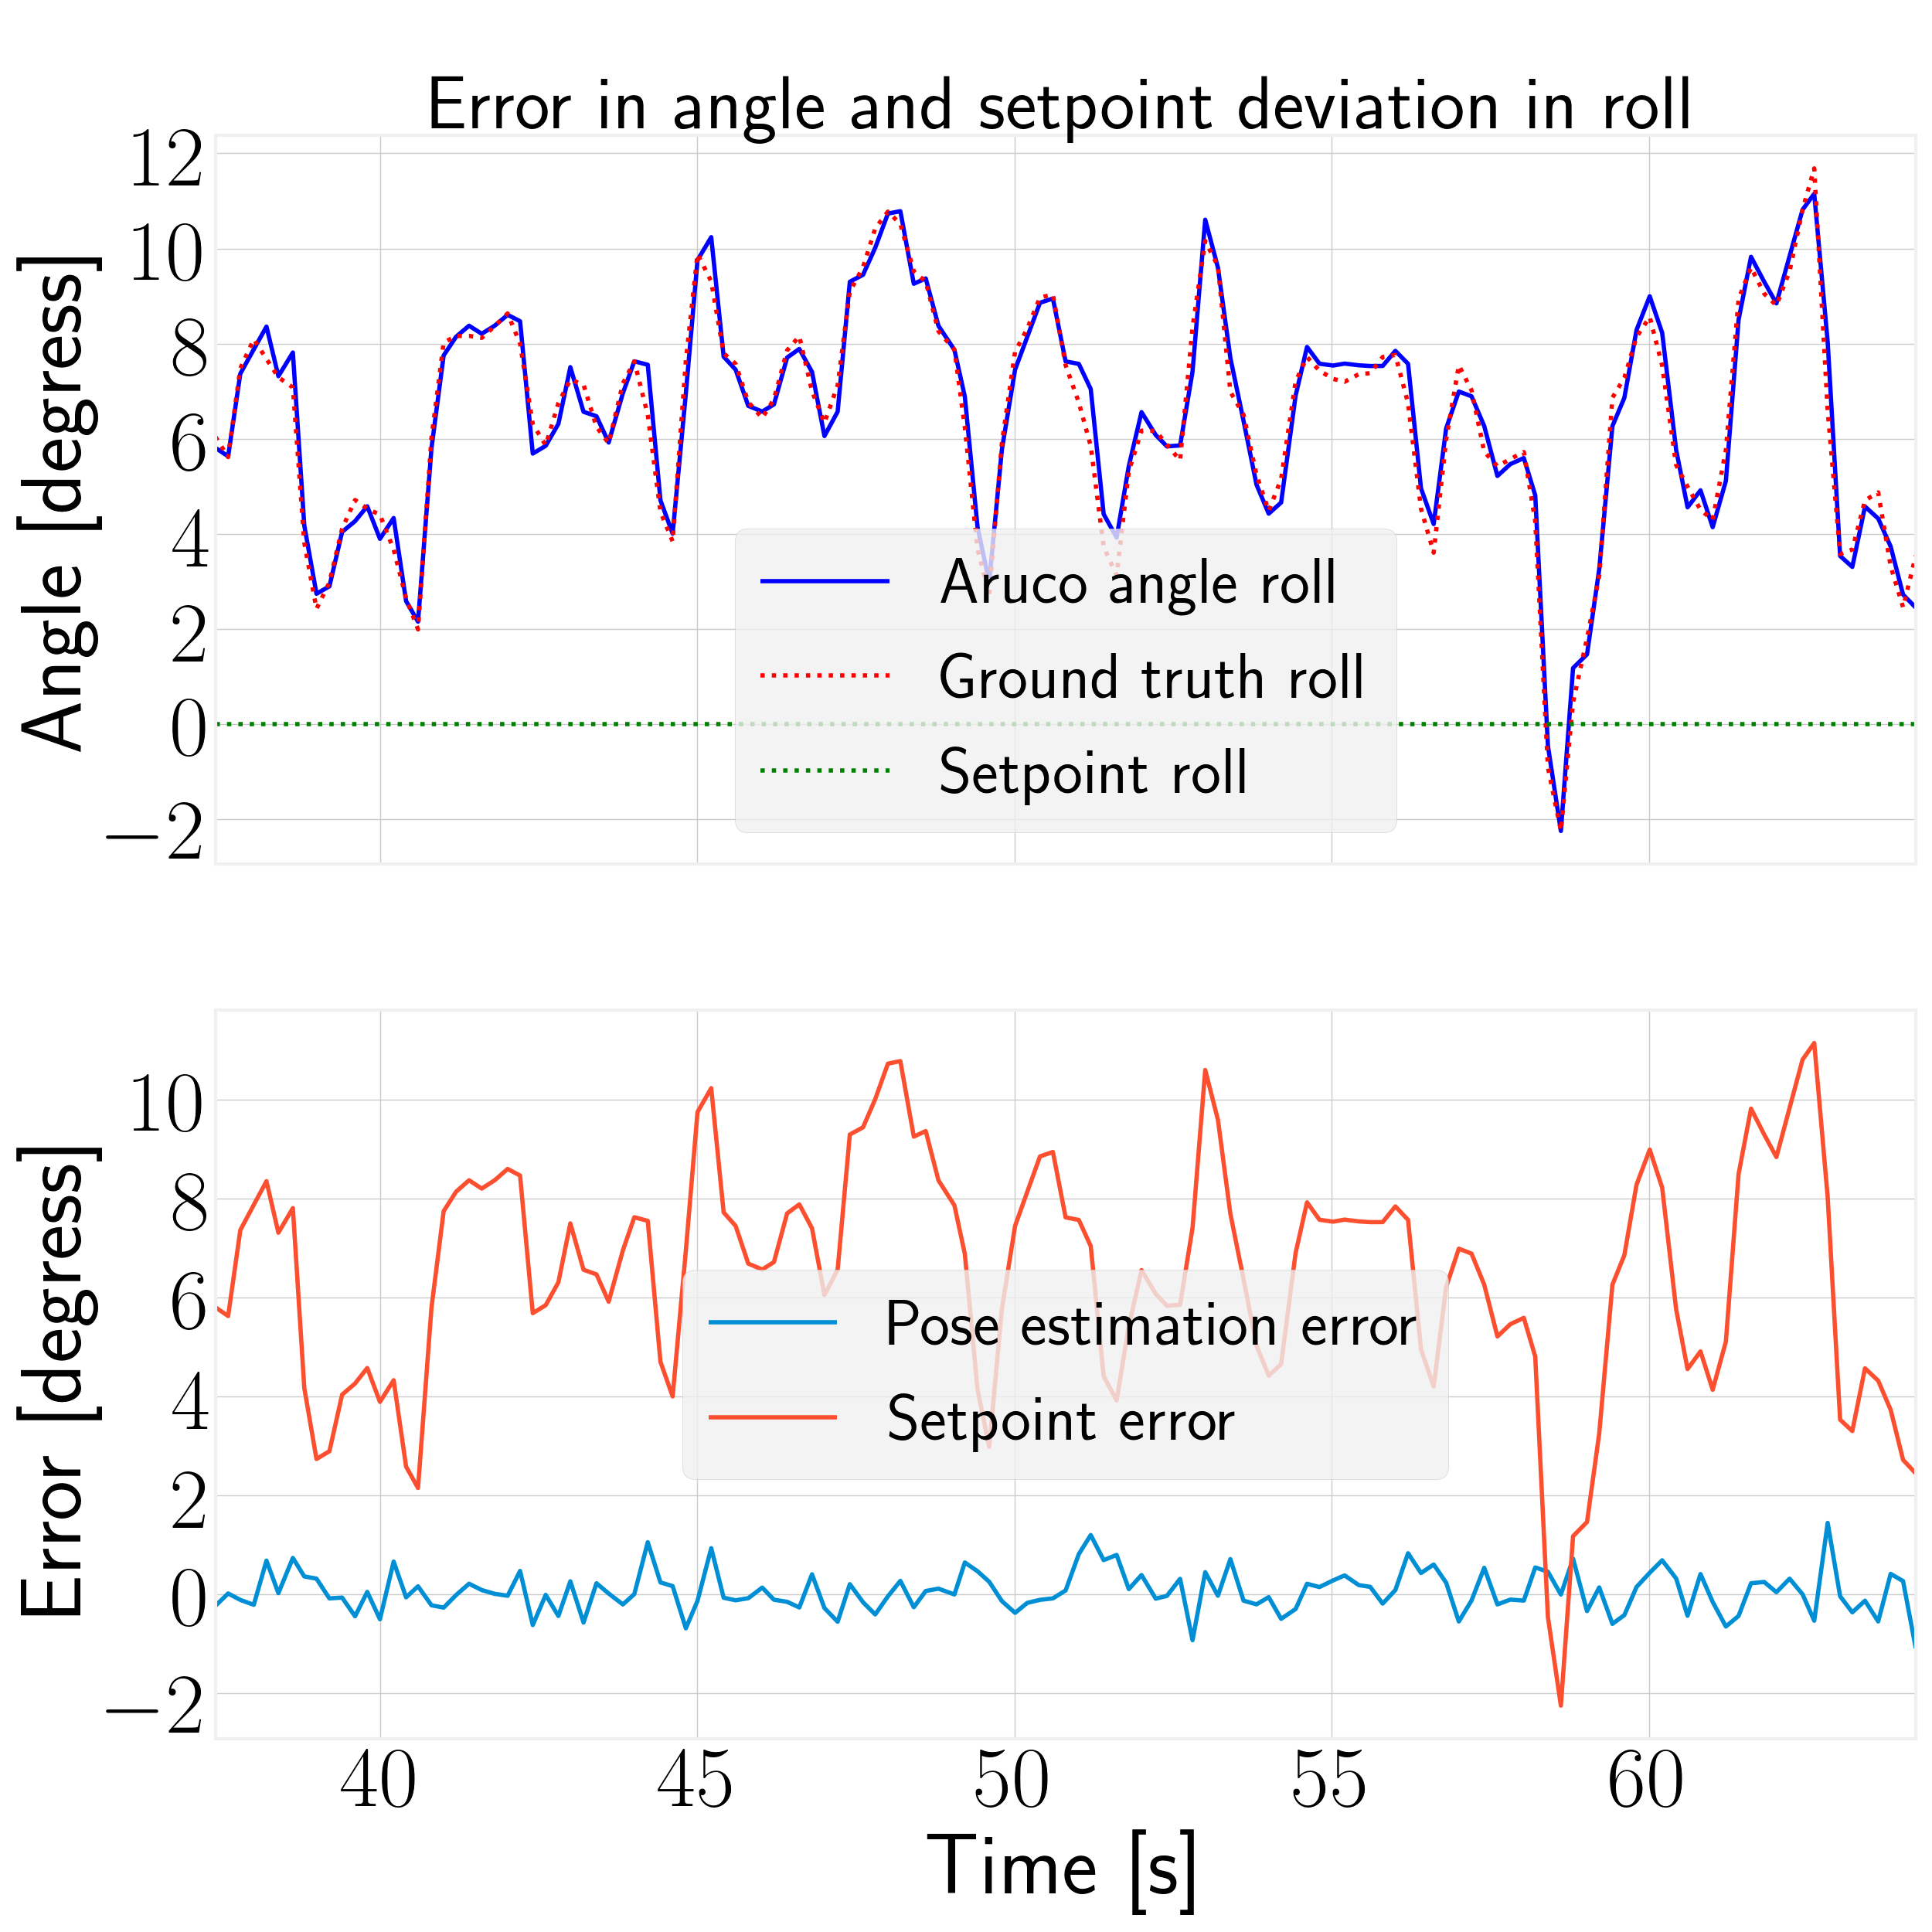
\includegraphics[width=\textwidth]{../Figures/hold_pose_using_aruco_pose_estimation/pose_error_roll_test2.png}
        \caption{}
        \label{fig:hold_pose_estimation_test2_roll}
    \end{subfigure}
     \hspace{0.2em}
    \begin{subfigure}[t]{.30\textwidth}
        \centering
        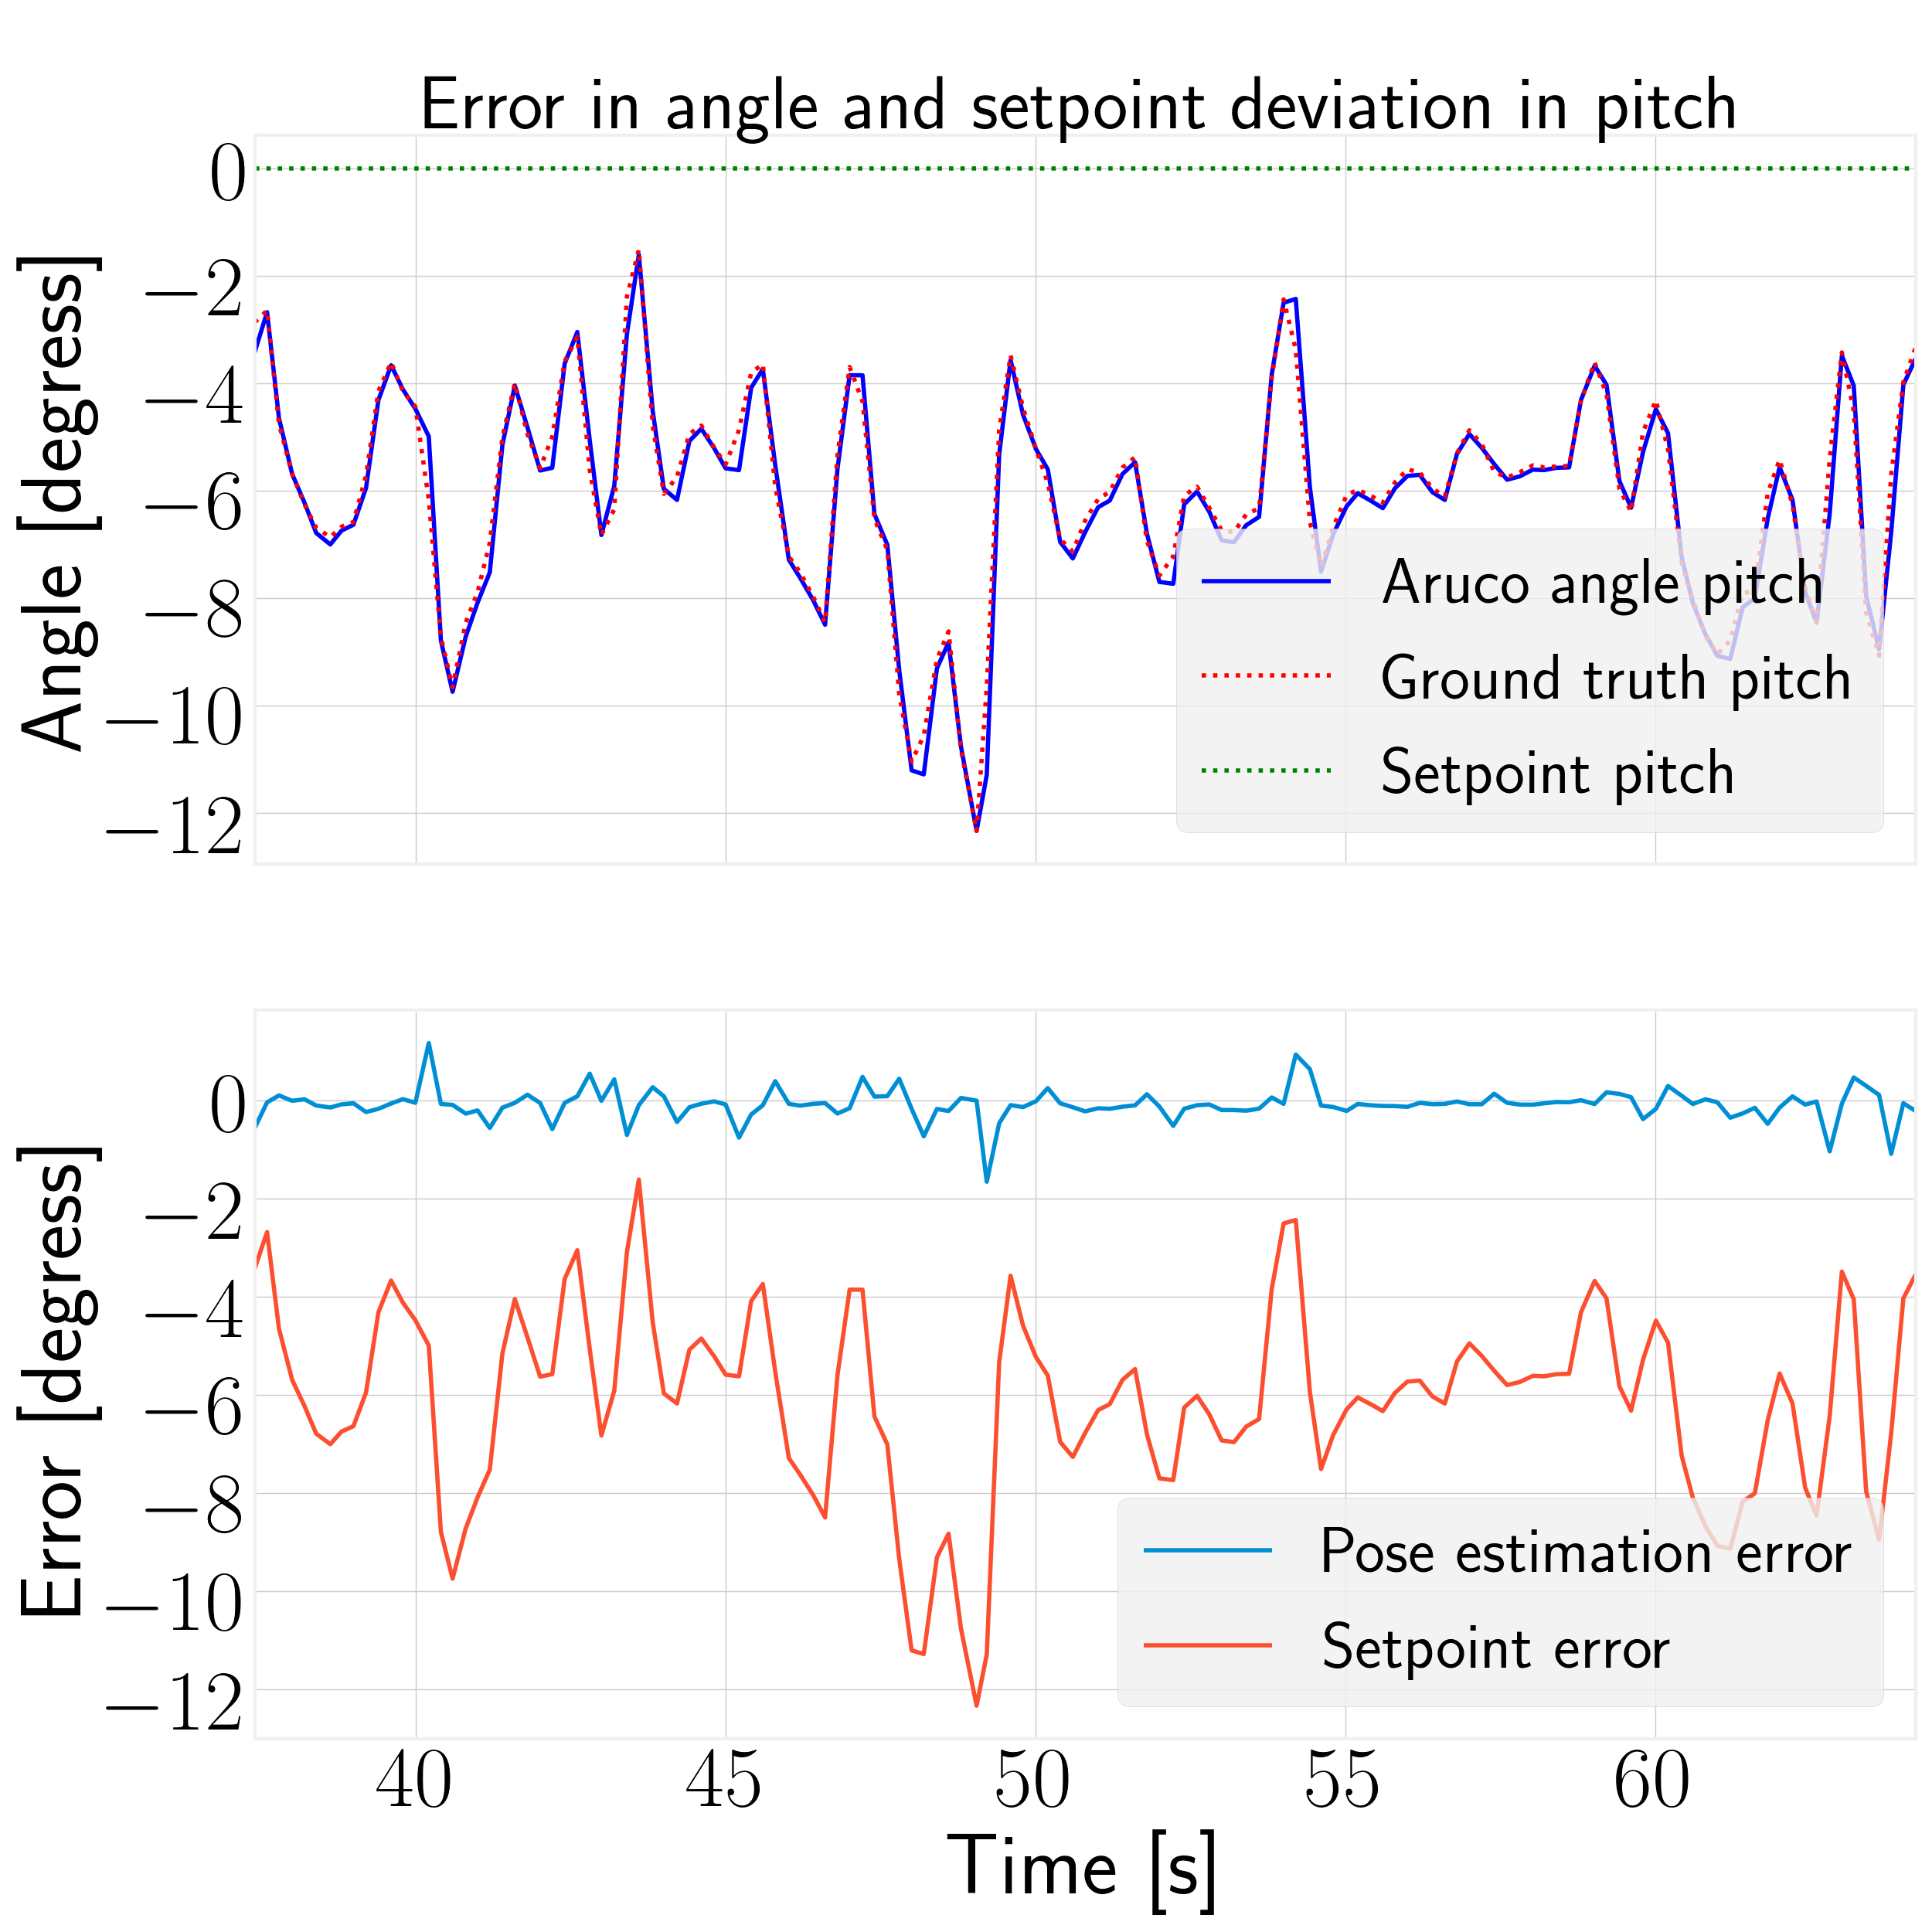
\includegraphics[width=\textwidth]{../Figures//hold_pose_using_aruco_pose_estimation/pose_error_pitch_test2.png}
        \caption{}
        \label{fig:hold_pose_estimation_test2_pitch}
    \end{subfigure}
     \hspace{0.2em}
    \begin{subfigure}[t]{.30\textwidth}
        \centering
        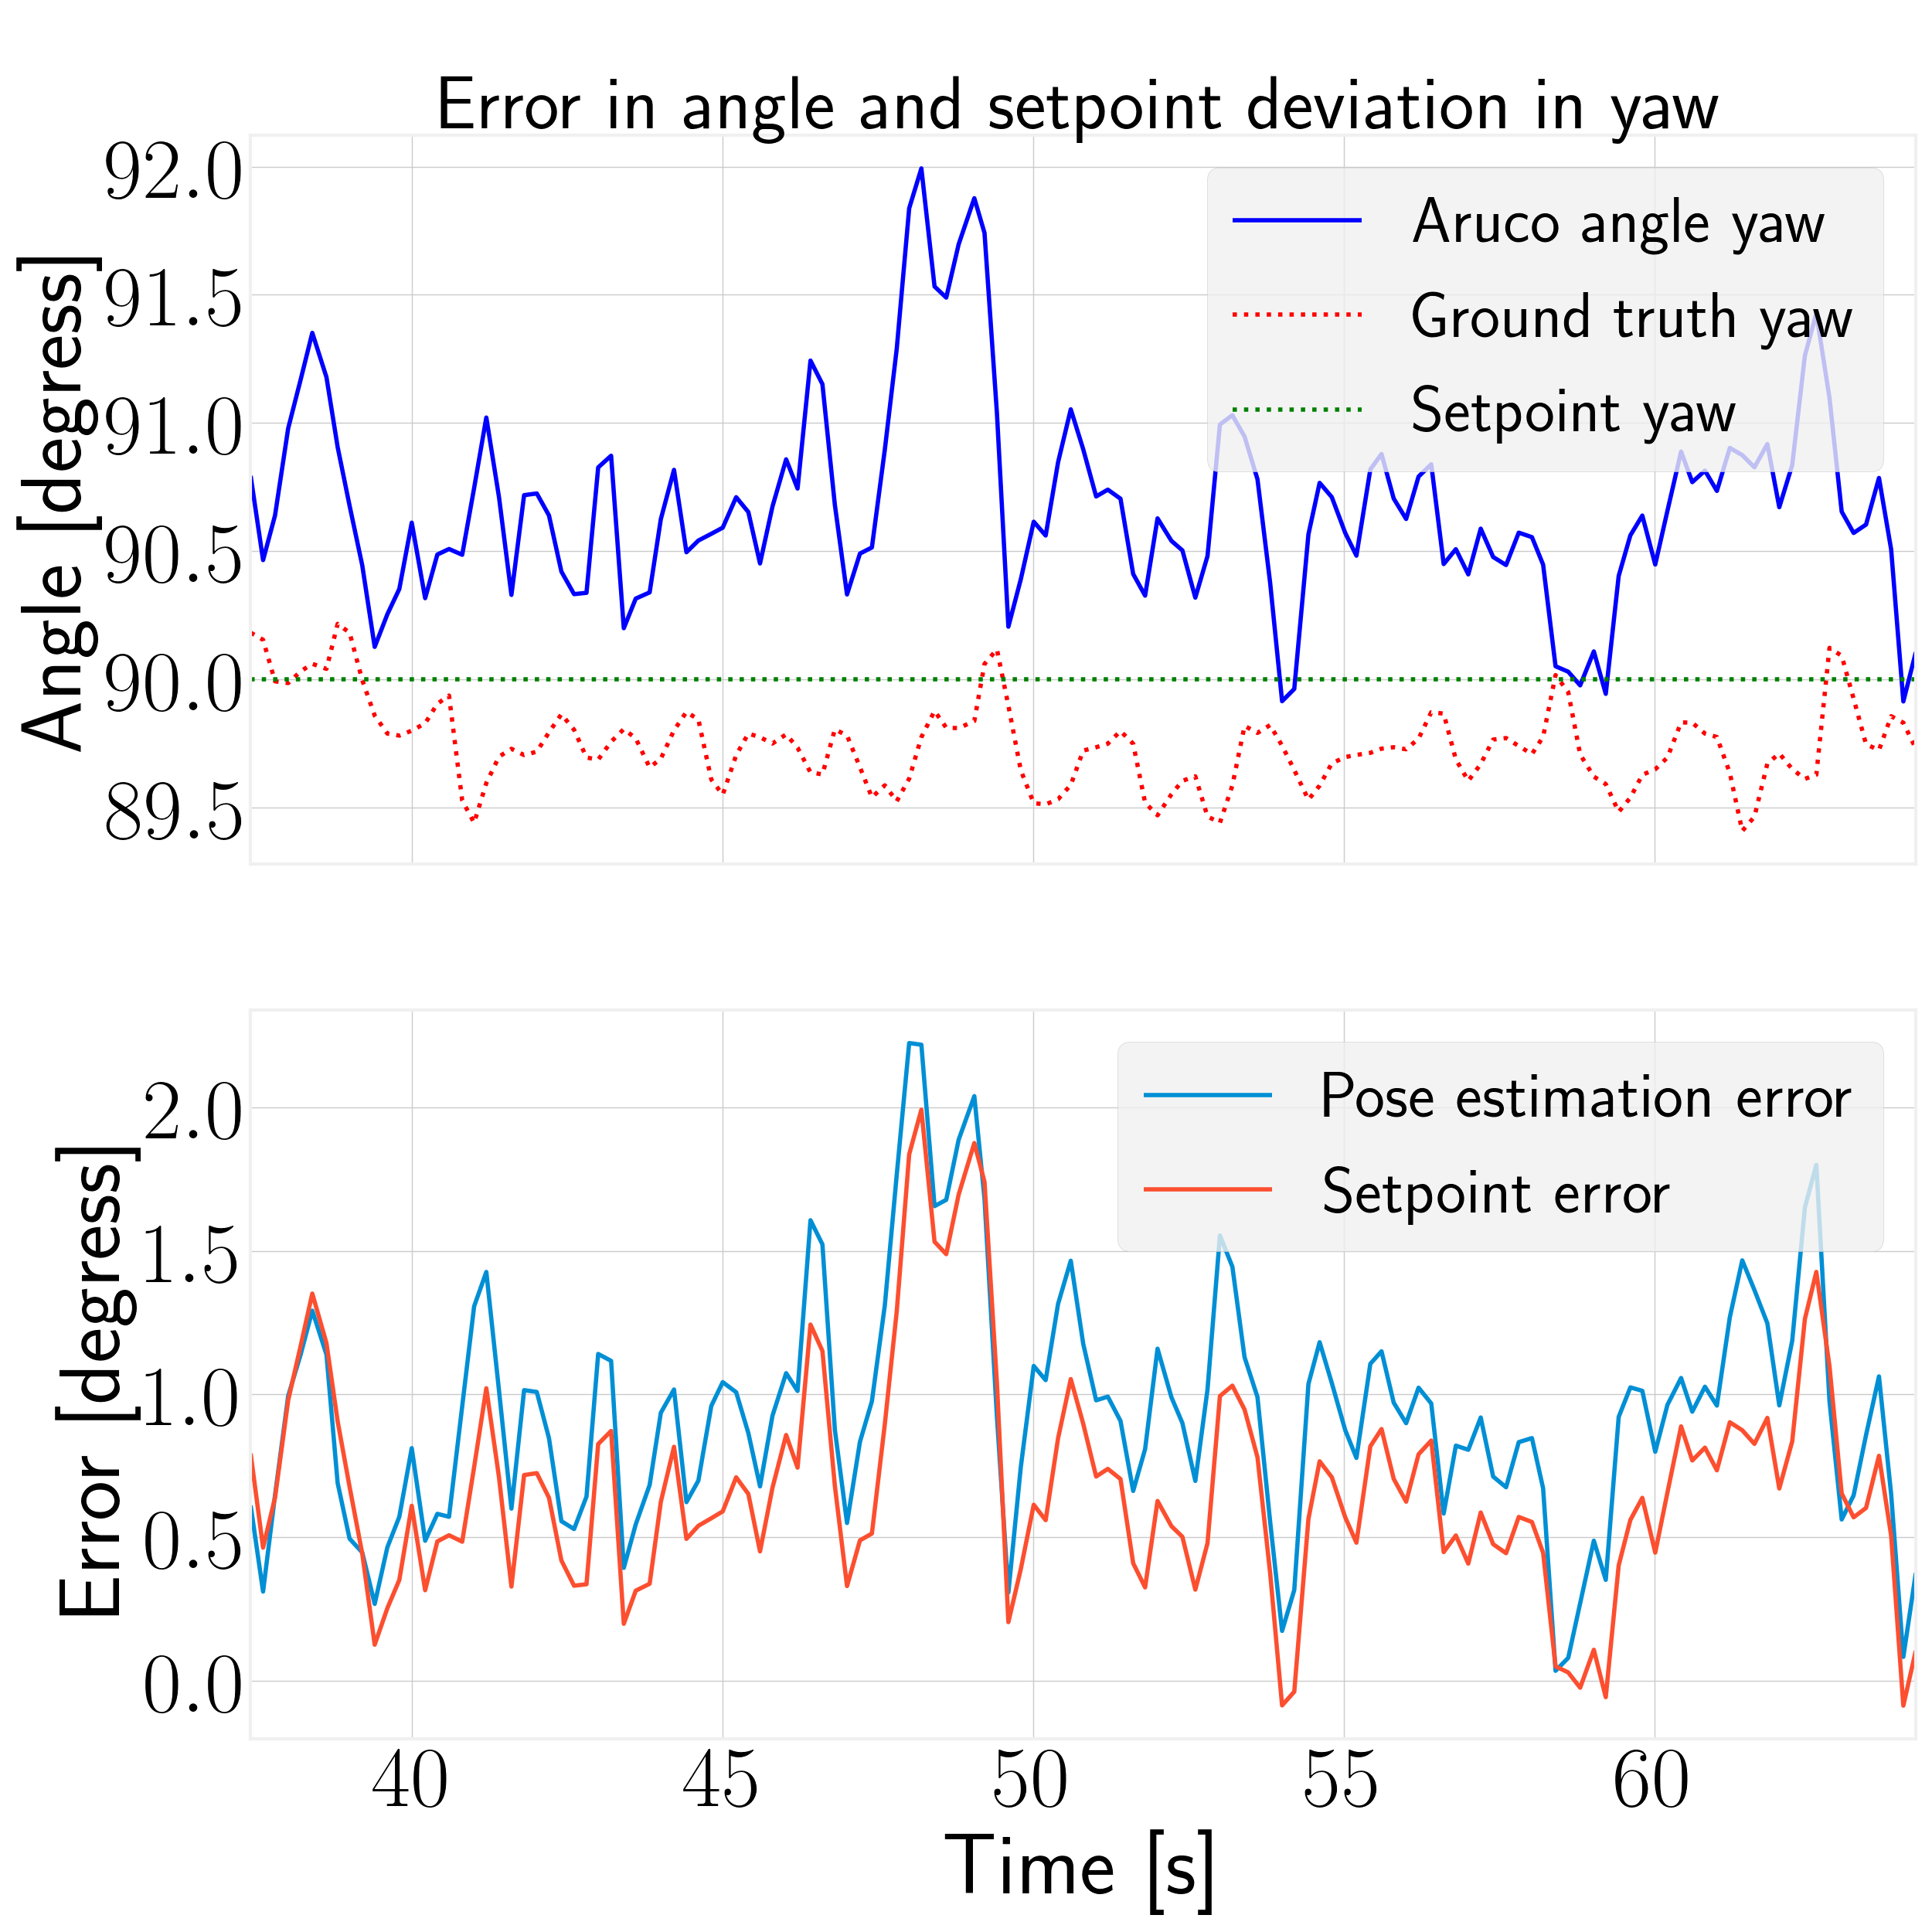
\includegraphics[width=\textwidth]{../Figures/hold_pose_using_aruco_pose_estimation/pose_error_yaw_test2.png}
        \caption{}
        \label{fig:hold_pose_estimation_test2_yaw}
    \end{subfigure}
    \caption{Illustration of the pose estimation and setpoint error using configuration in Figure \ref{fig:hold_pose_aruco_board_one_5-7ms_wind}. It may be noticed that the UAV has trouble keeping roll and pitch close to zero due to the wind in the simulation in Figures \ref{fig:hold_pose_estimation_test2_roll} and \ref{fig:hold_pose_estimation_test2_pitch}}
    \label{fig:hold_pose_estimation_test2_error_angle}
\end{figure}

\begin{figure}[H]
    \centering
    \begin{subfigure}[t]{.30\textwidth}
        \centering
        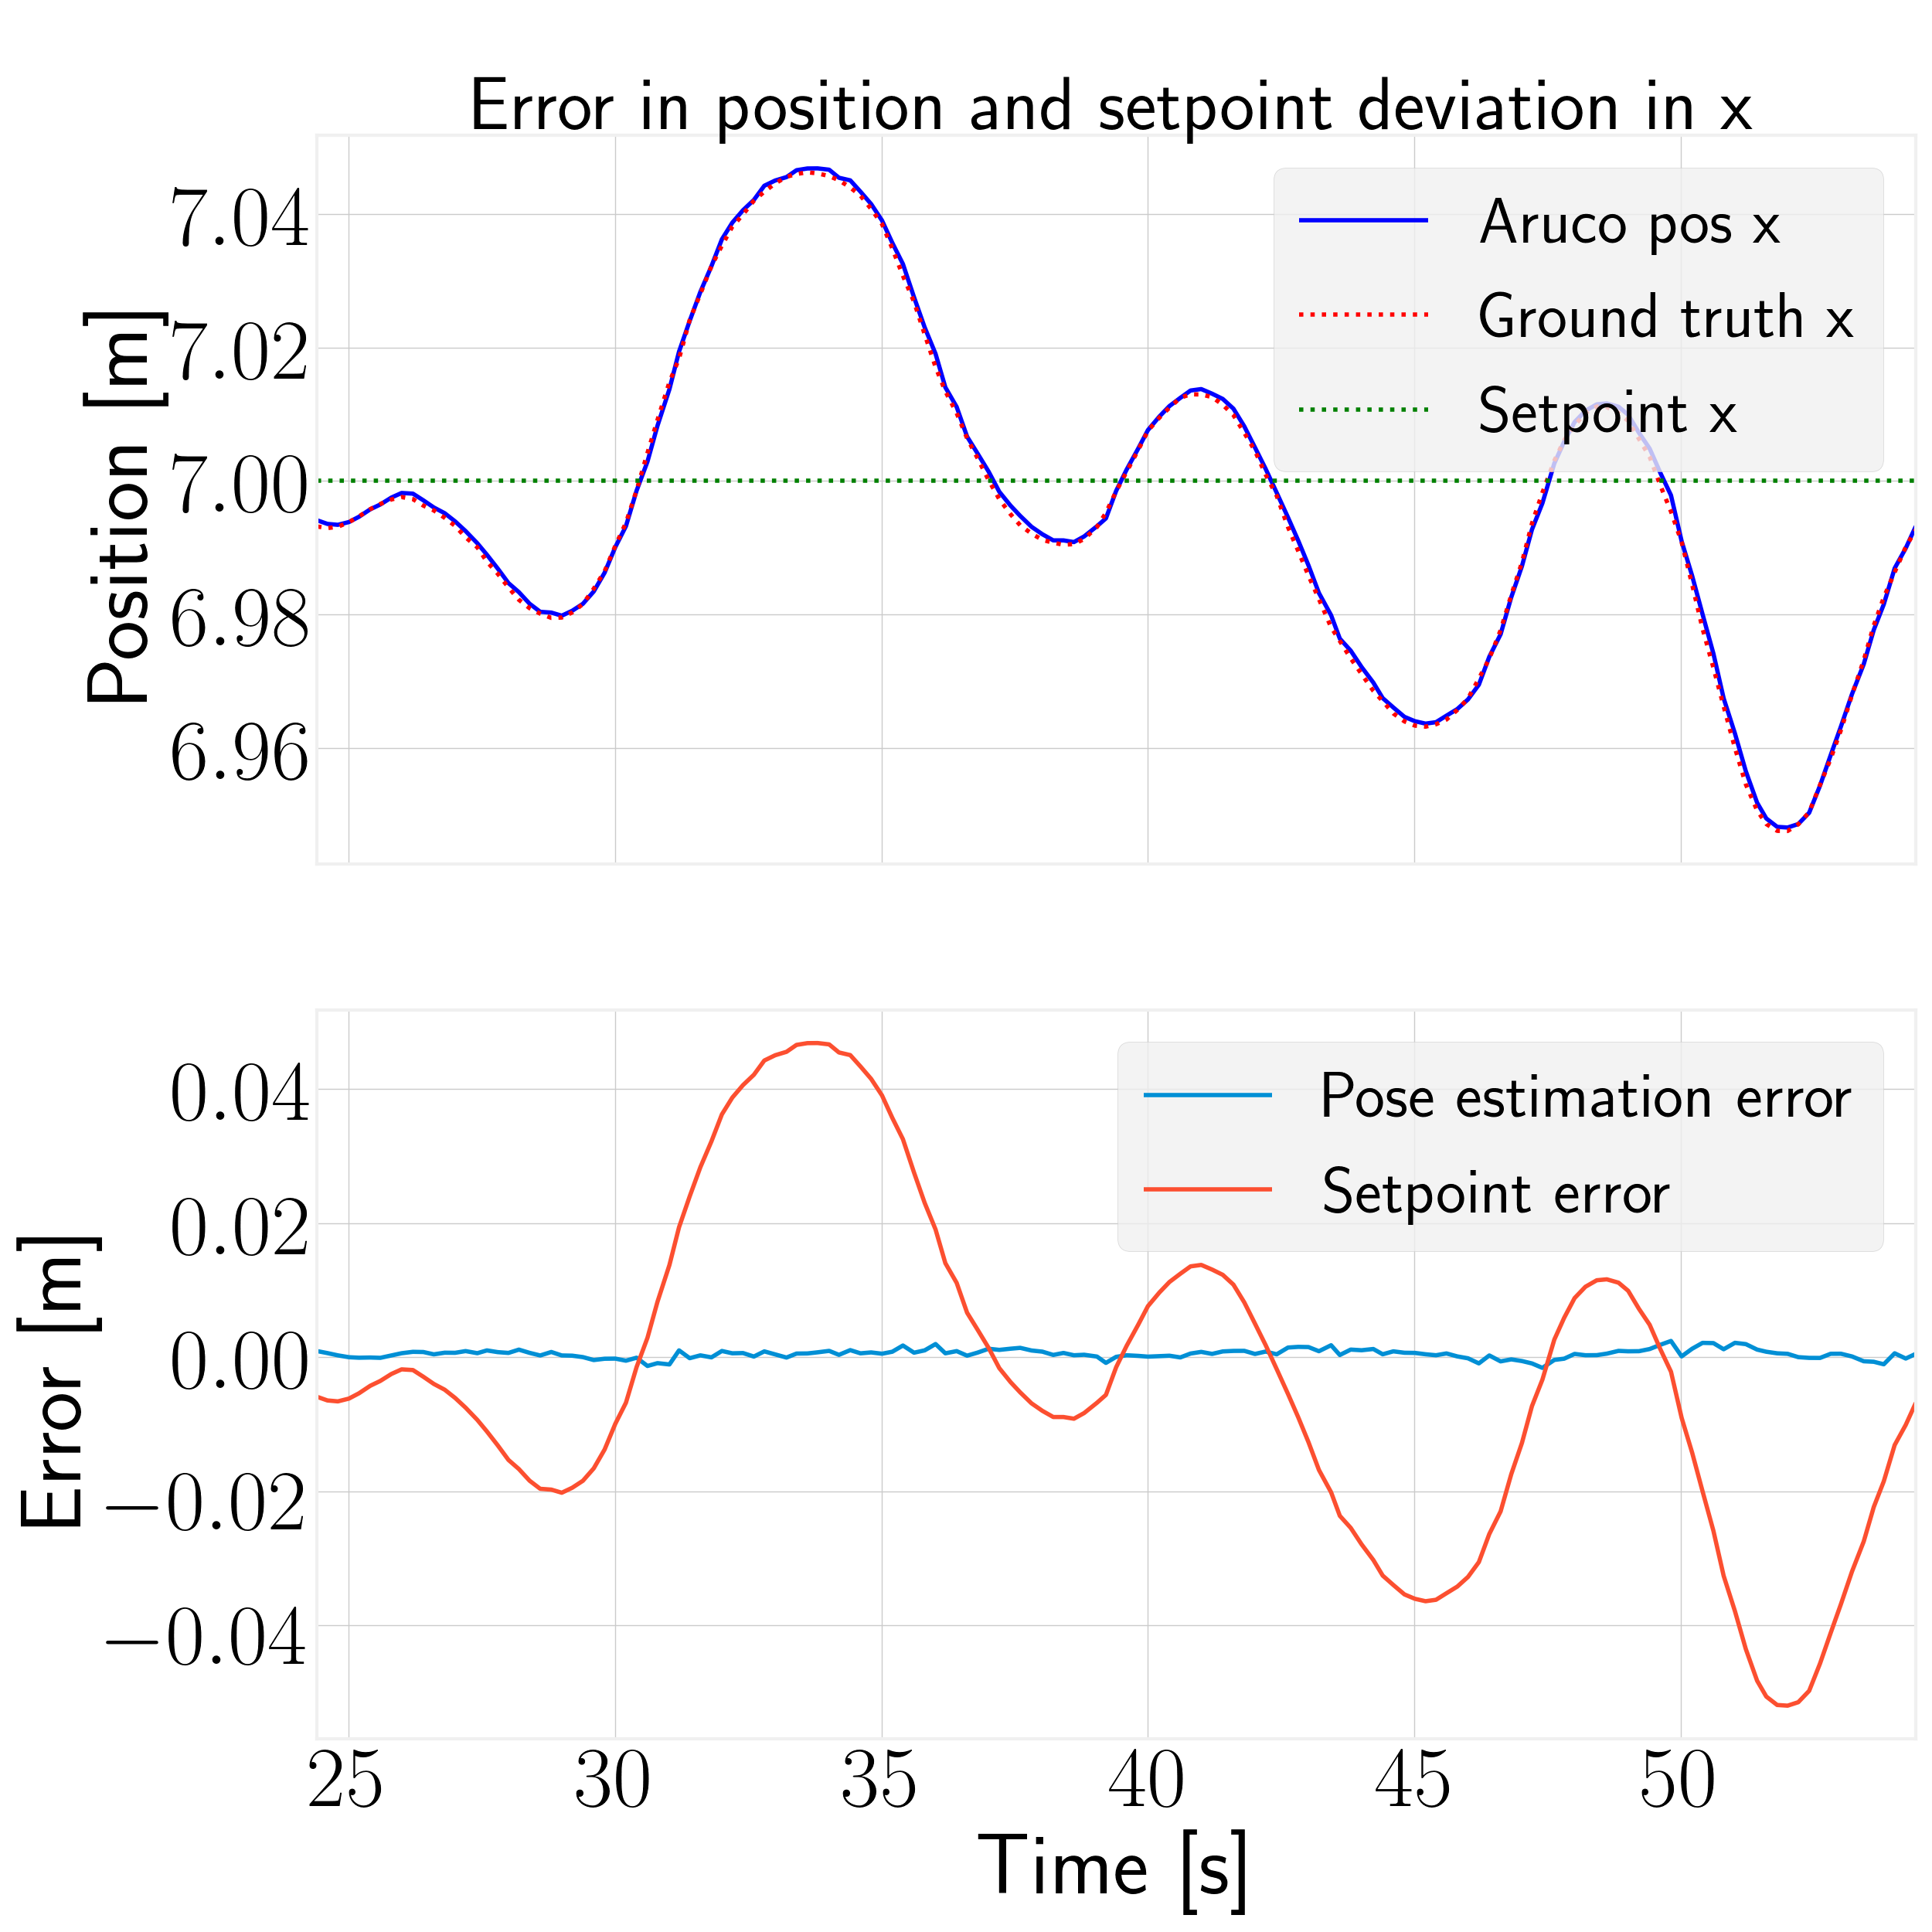
\includegraphics[width=\textwidth]{../Figures/hold_pose_using_aruco_pose_estimation/pose_error_x_test1.png}
        \caption{}
        \label{fig:hold_pose_estimation_test5_x}
    \end{subfigure}
     \hspace{0.2em}
    \begin{subfigure}[t]{.30\textwidth}
        \centering
        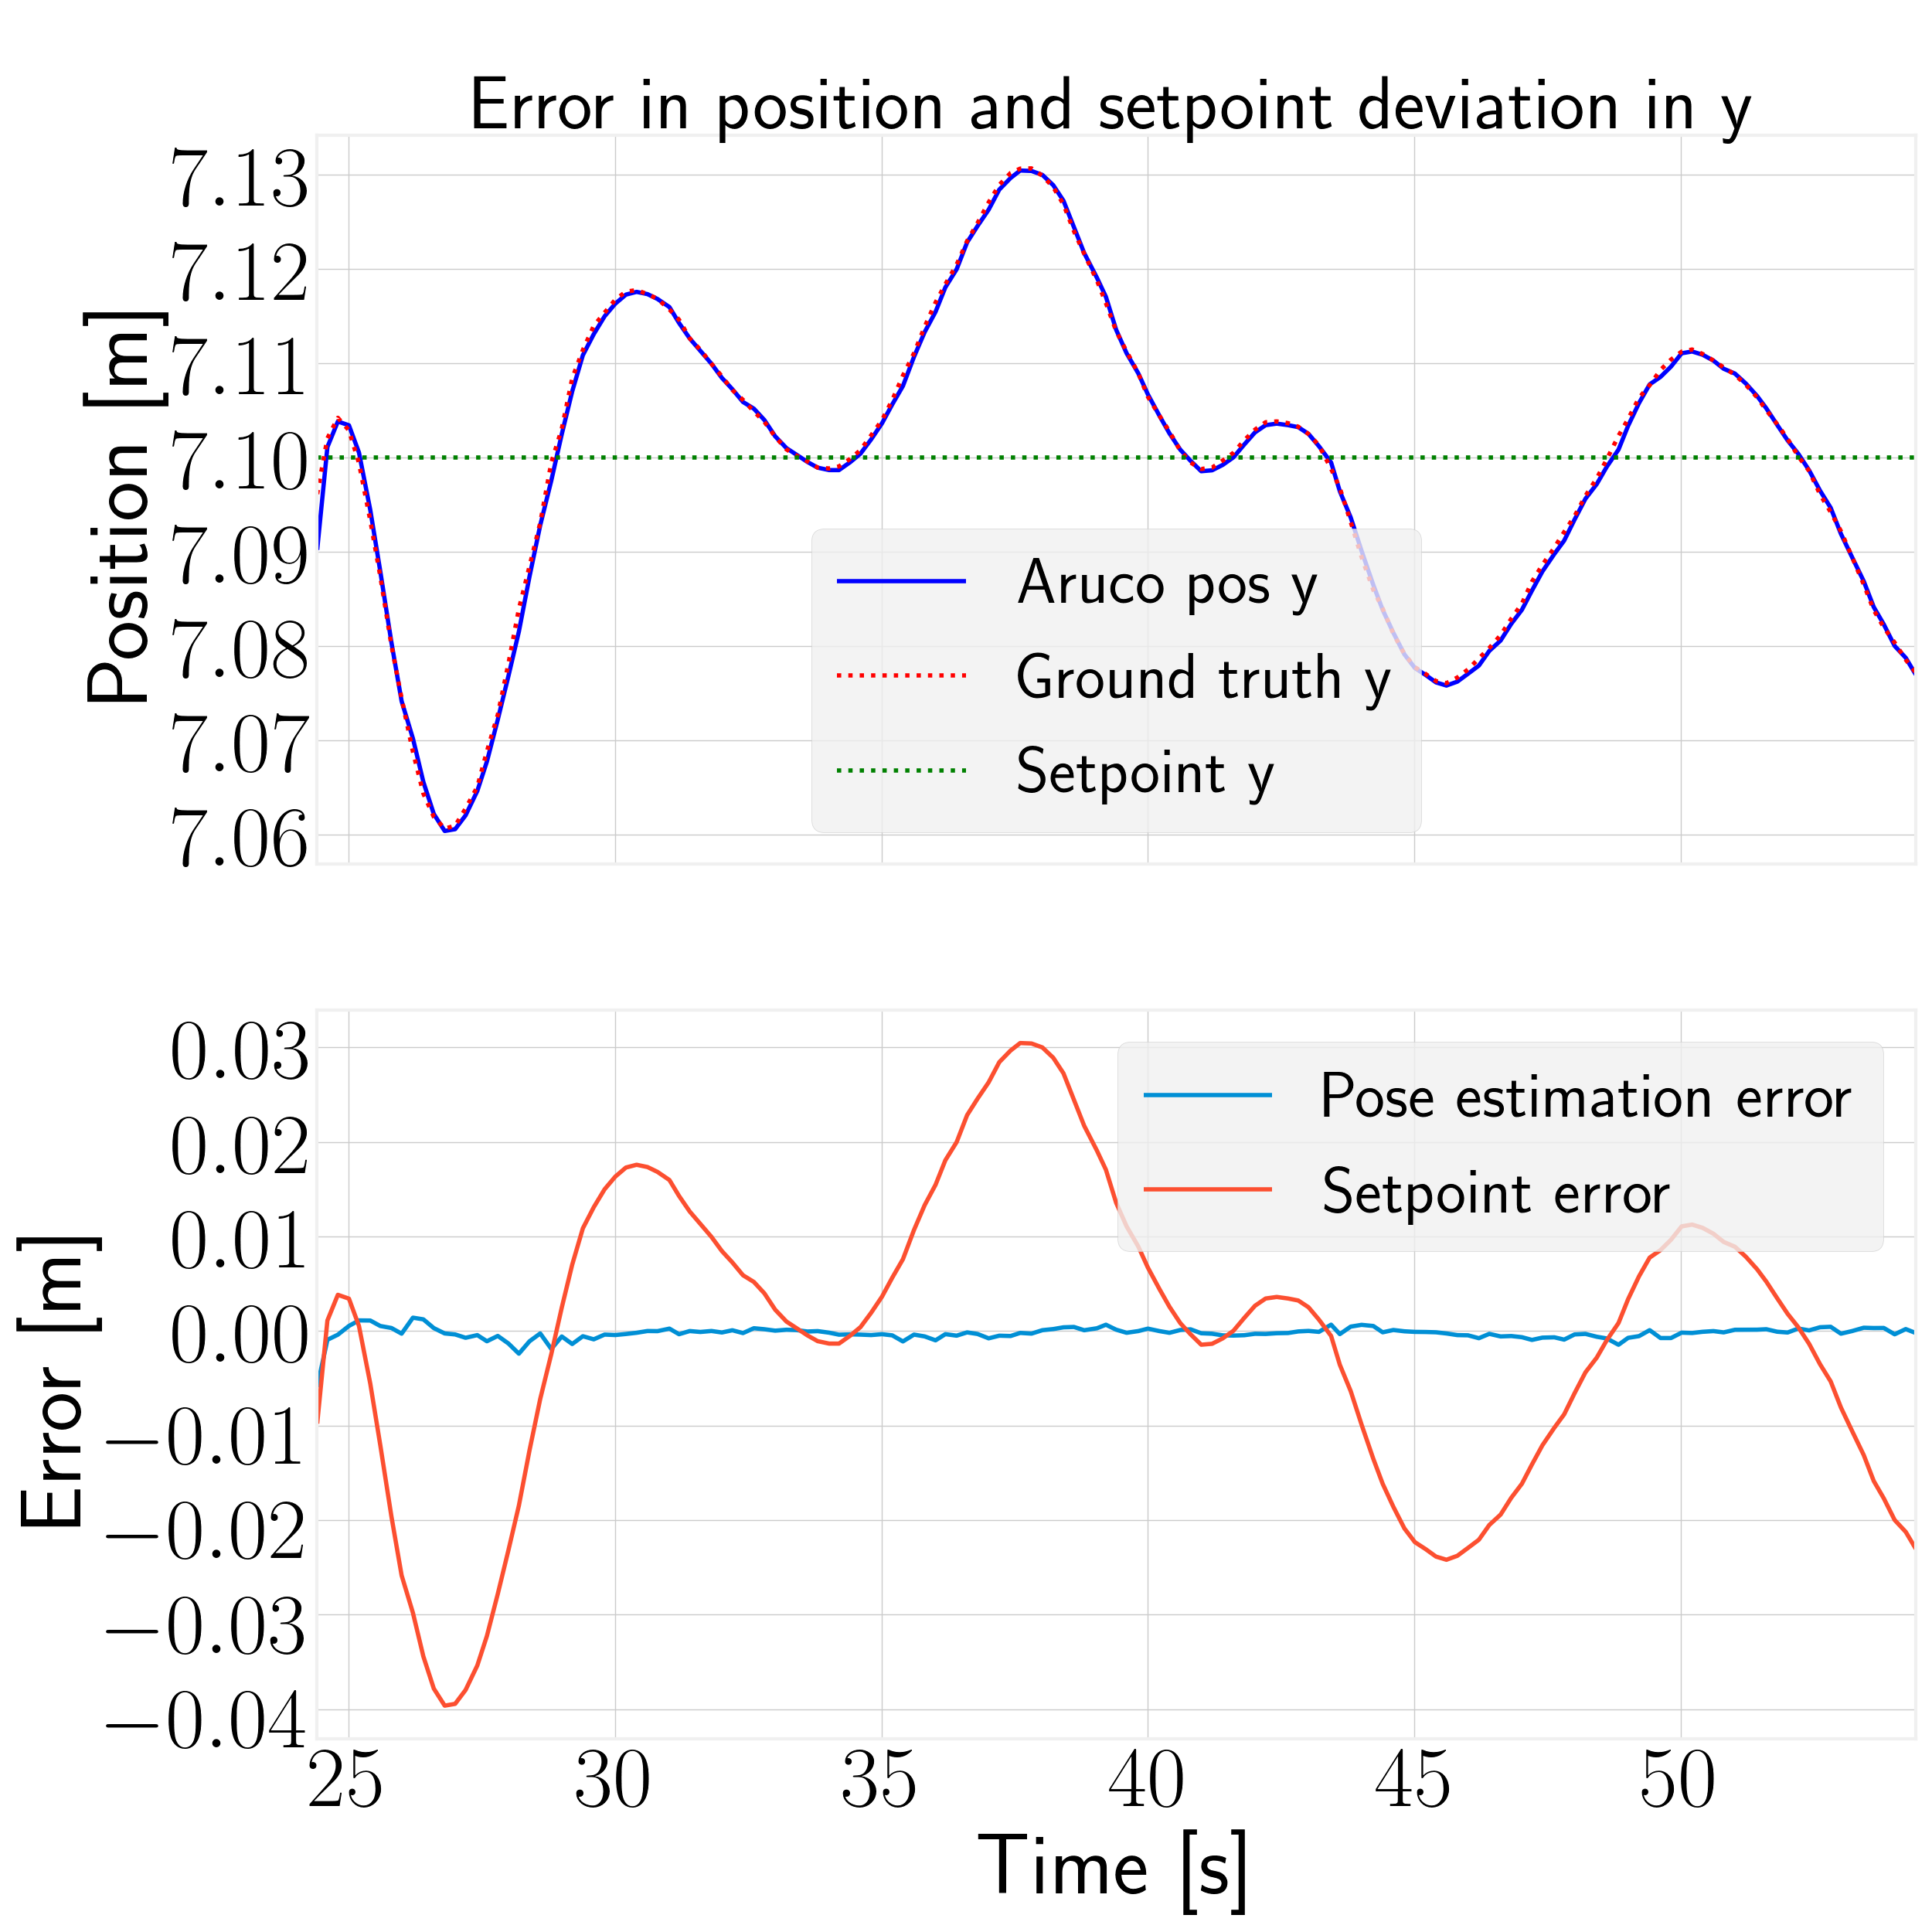
\includegraphics[width=\textwidth]{../Figures/hold_pose_using_aruco_pose_estimation/pose_error_y_test1.png}
        \caption{}
        \label{fig:hold_pose_estimation_test5_y}
    \end{subfigure}
     \hspace{0.2em}
    \begin{subfigure}[t]{.30\textwidth}
        \centering
        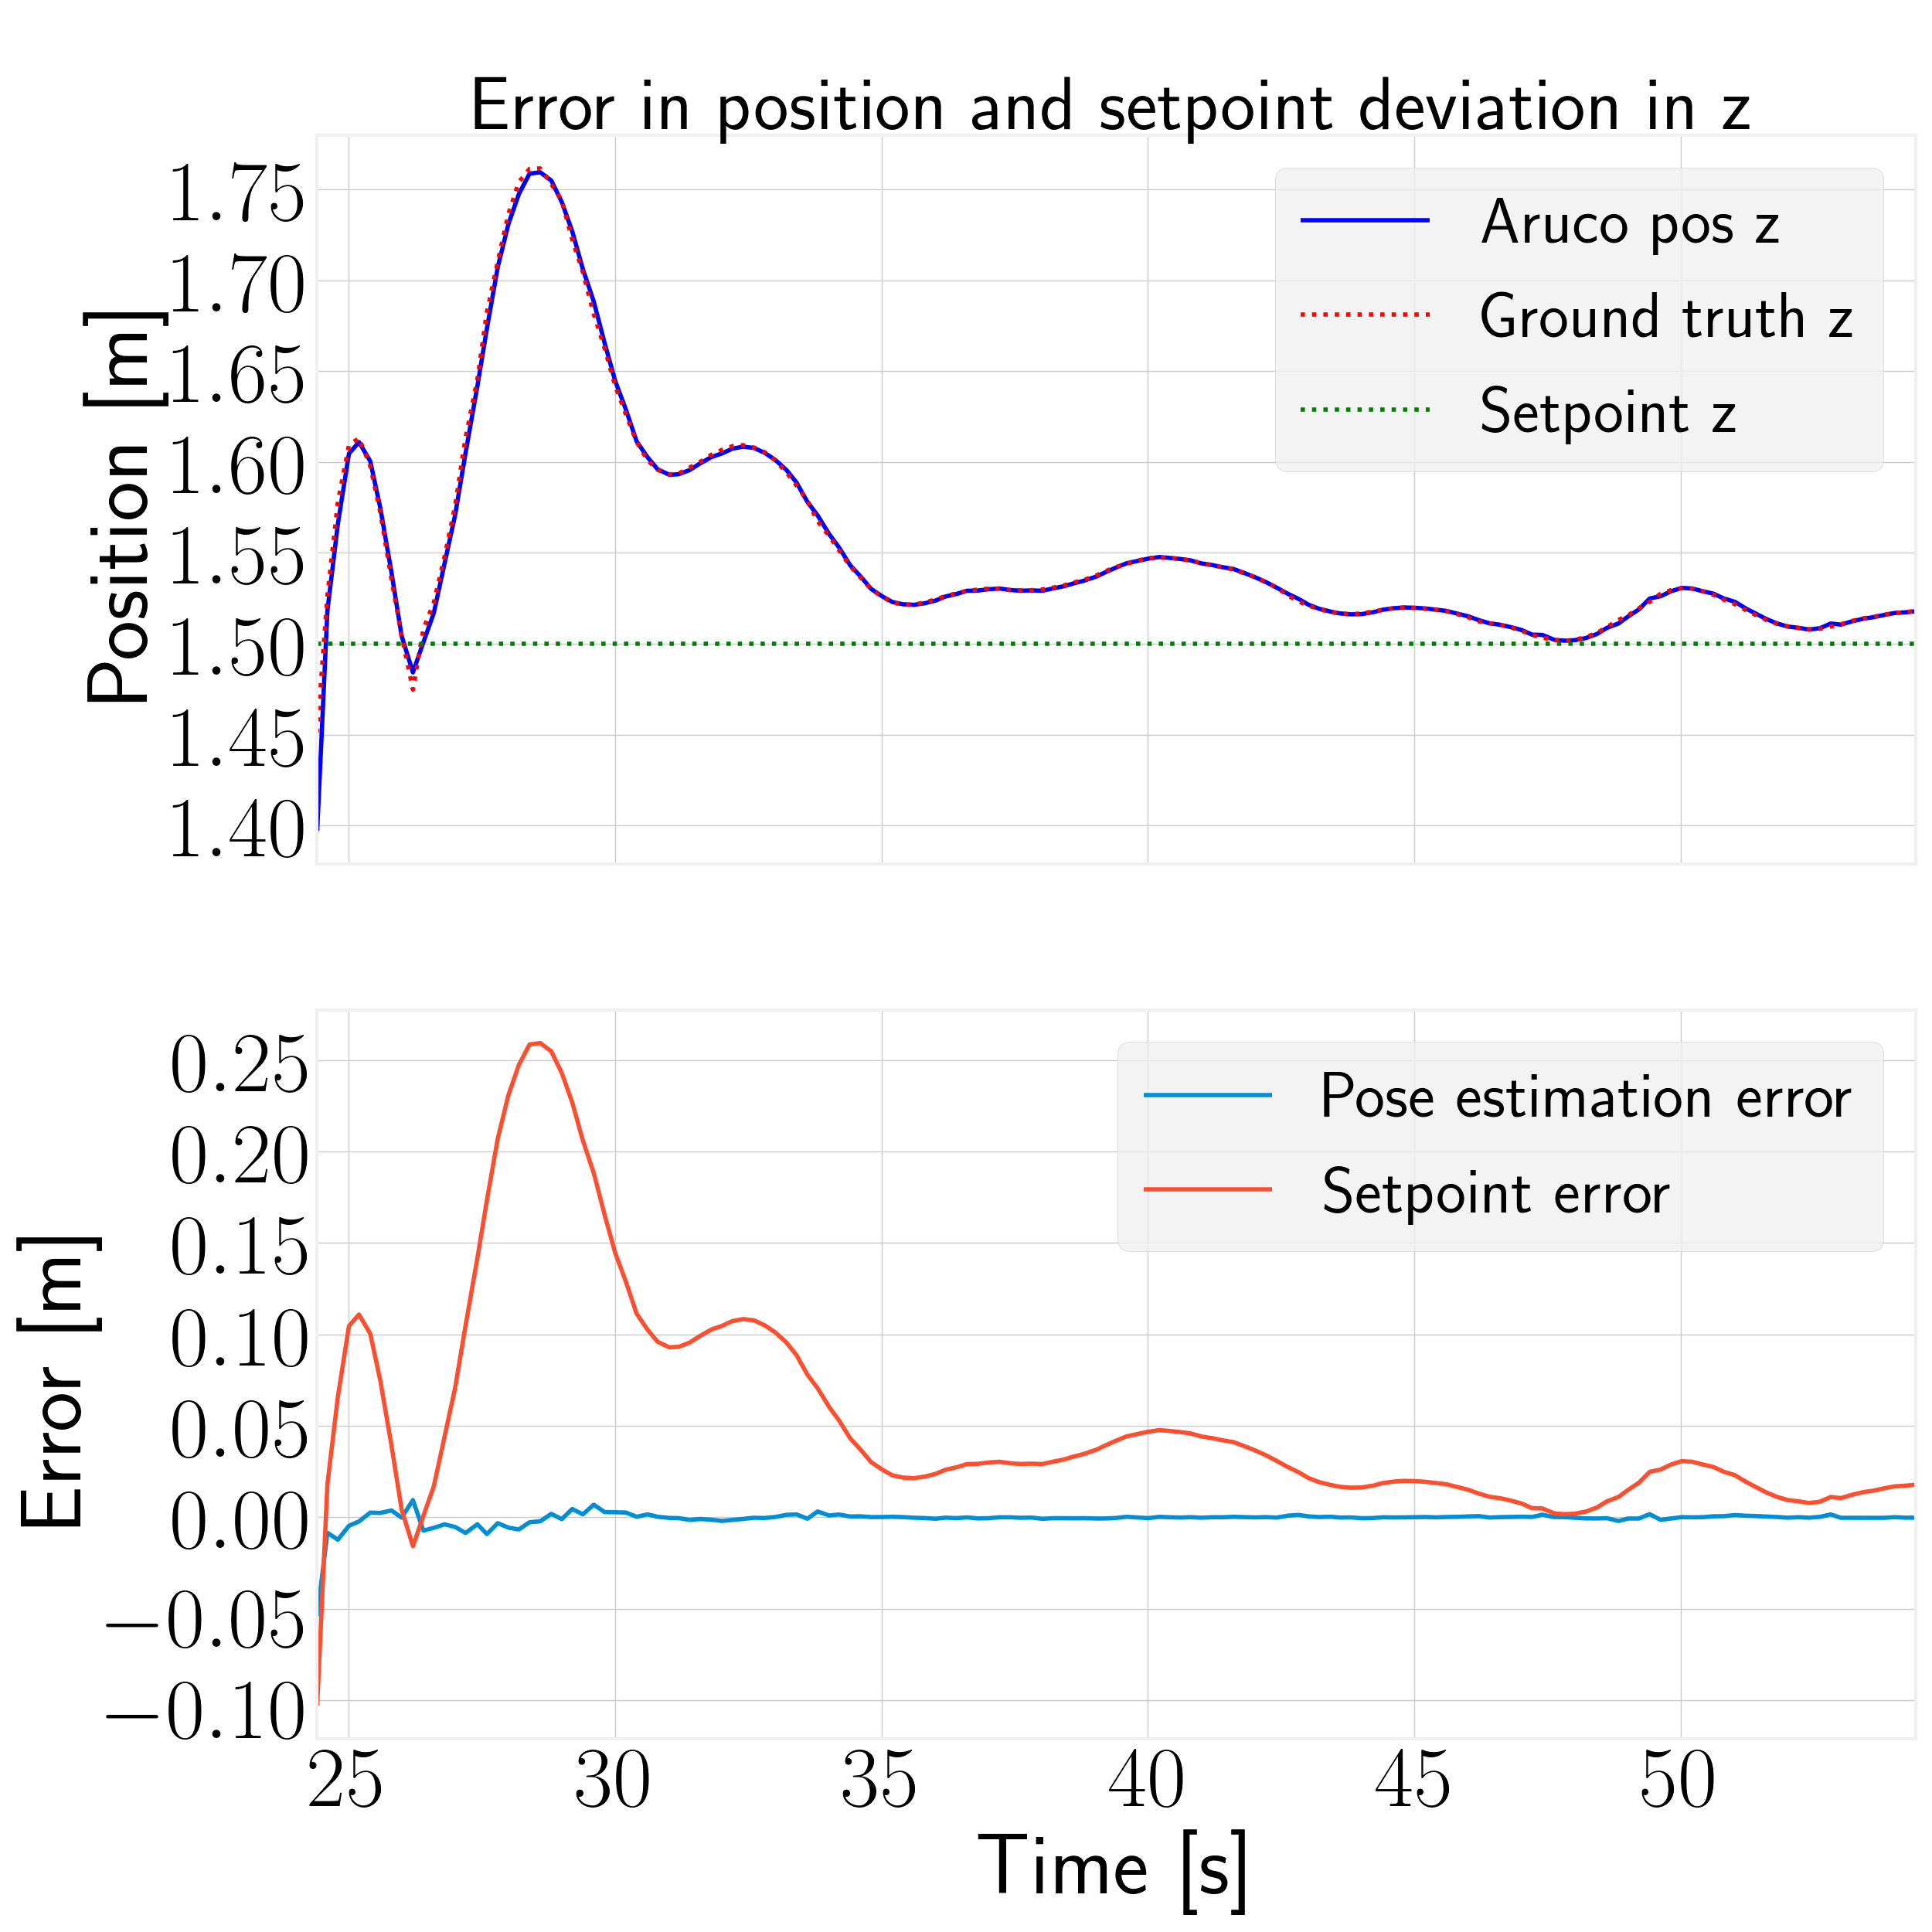
\includegraphics[width=\textwidth]{../Figures/hold_pose_using_aruco_pose_estimation/pose_error_z_test1.png}
        \caption{}
        \label{fig:hold_pose_estimation_test5_z}
    \end{subfigure}
    \caption{Illustration of the pose estimation and setpoint error using configuration in Figure \ref{fig:hold_pose_aruco_board_five}. It can be seen that the error in position estimation is almost negligible down to millimeters of error which was also mentioned in Table \ref{tab:hold_pose_using_landing_station_boards}. Moreover, the setpoint error has decreased significantly which illustrates that the overall stability of the system increases when the UAV operates closer to the board}
    \label{fig:hold_pose_estimation_test5_error_pos}
\end{figure}

\begin{figure}[H]
    \centering
    \begin{subfigure}[t]{.30\textwidth}
        \centering
        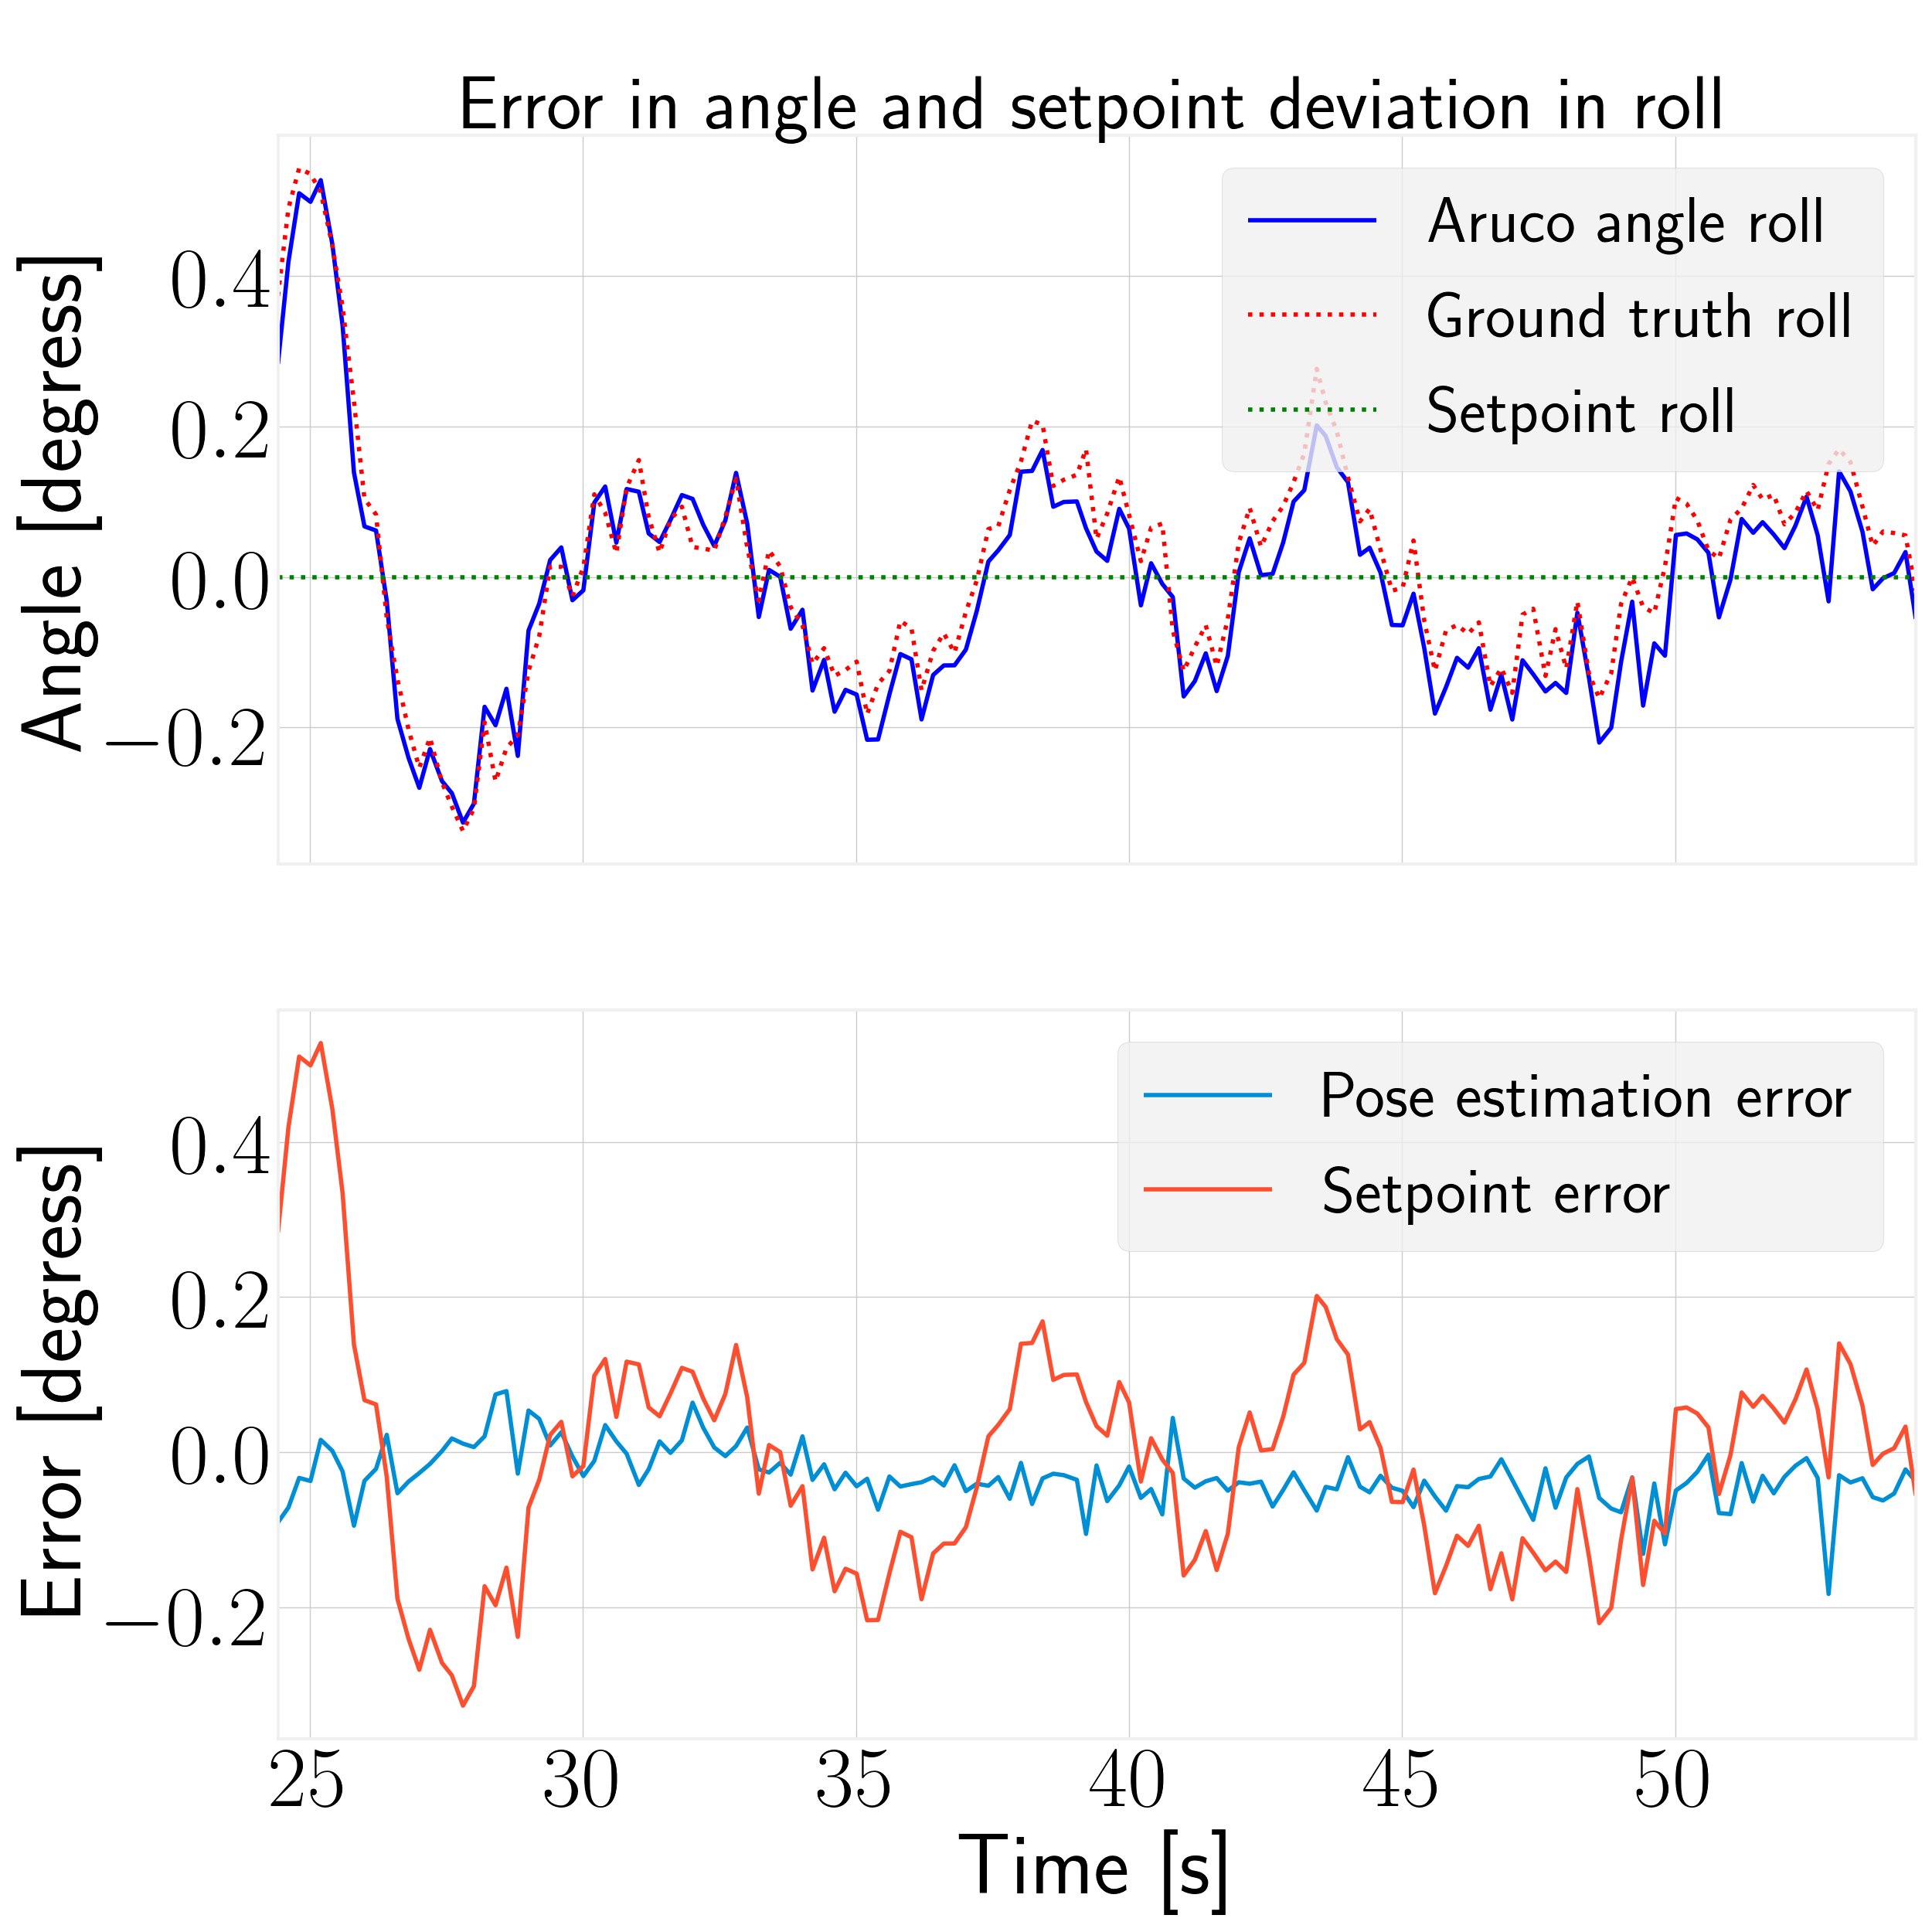
\includegraphics[width=\textwidth]{../Figures/hold_pose_using_aruco_pose_estimation/pose_error_roll_test1.png}
        \caption{}
        \label{fig:hold_pose_estimation_test5_roll}
    \end{subfigure}
     \hspace{0.2em}
    \begin{subfigure}[t]{.30\textwidth}
        \centering
        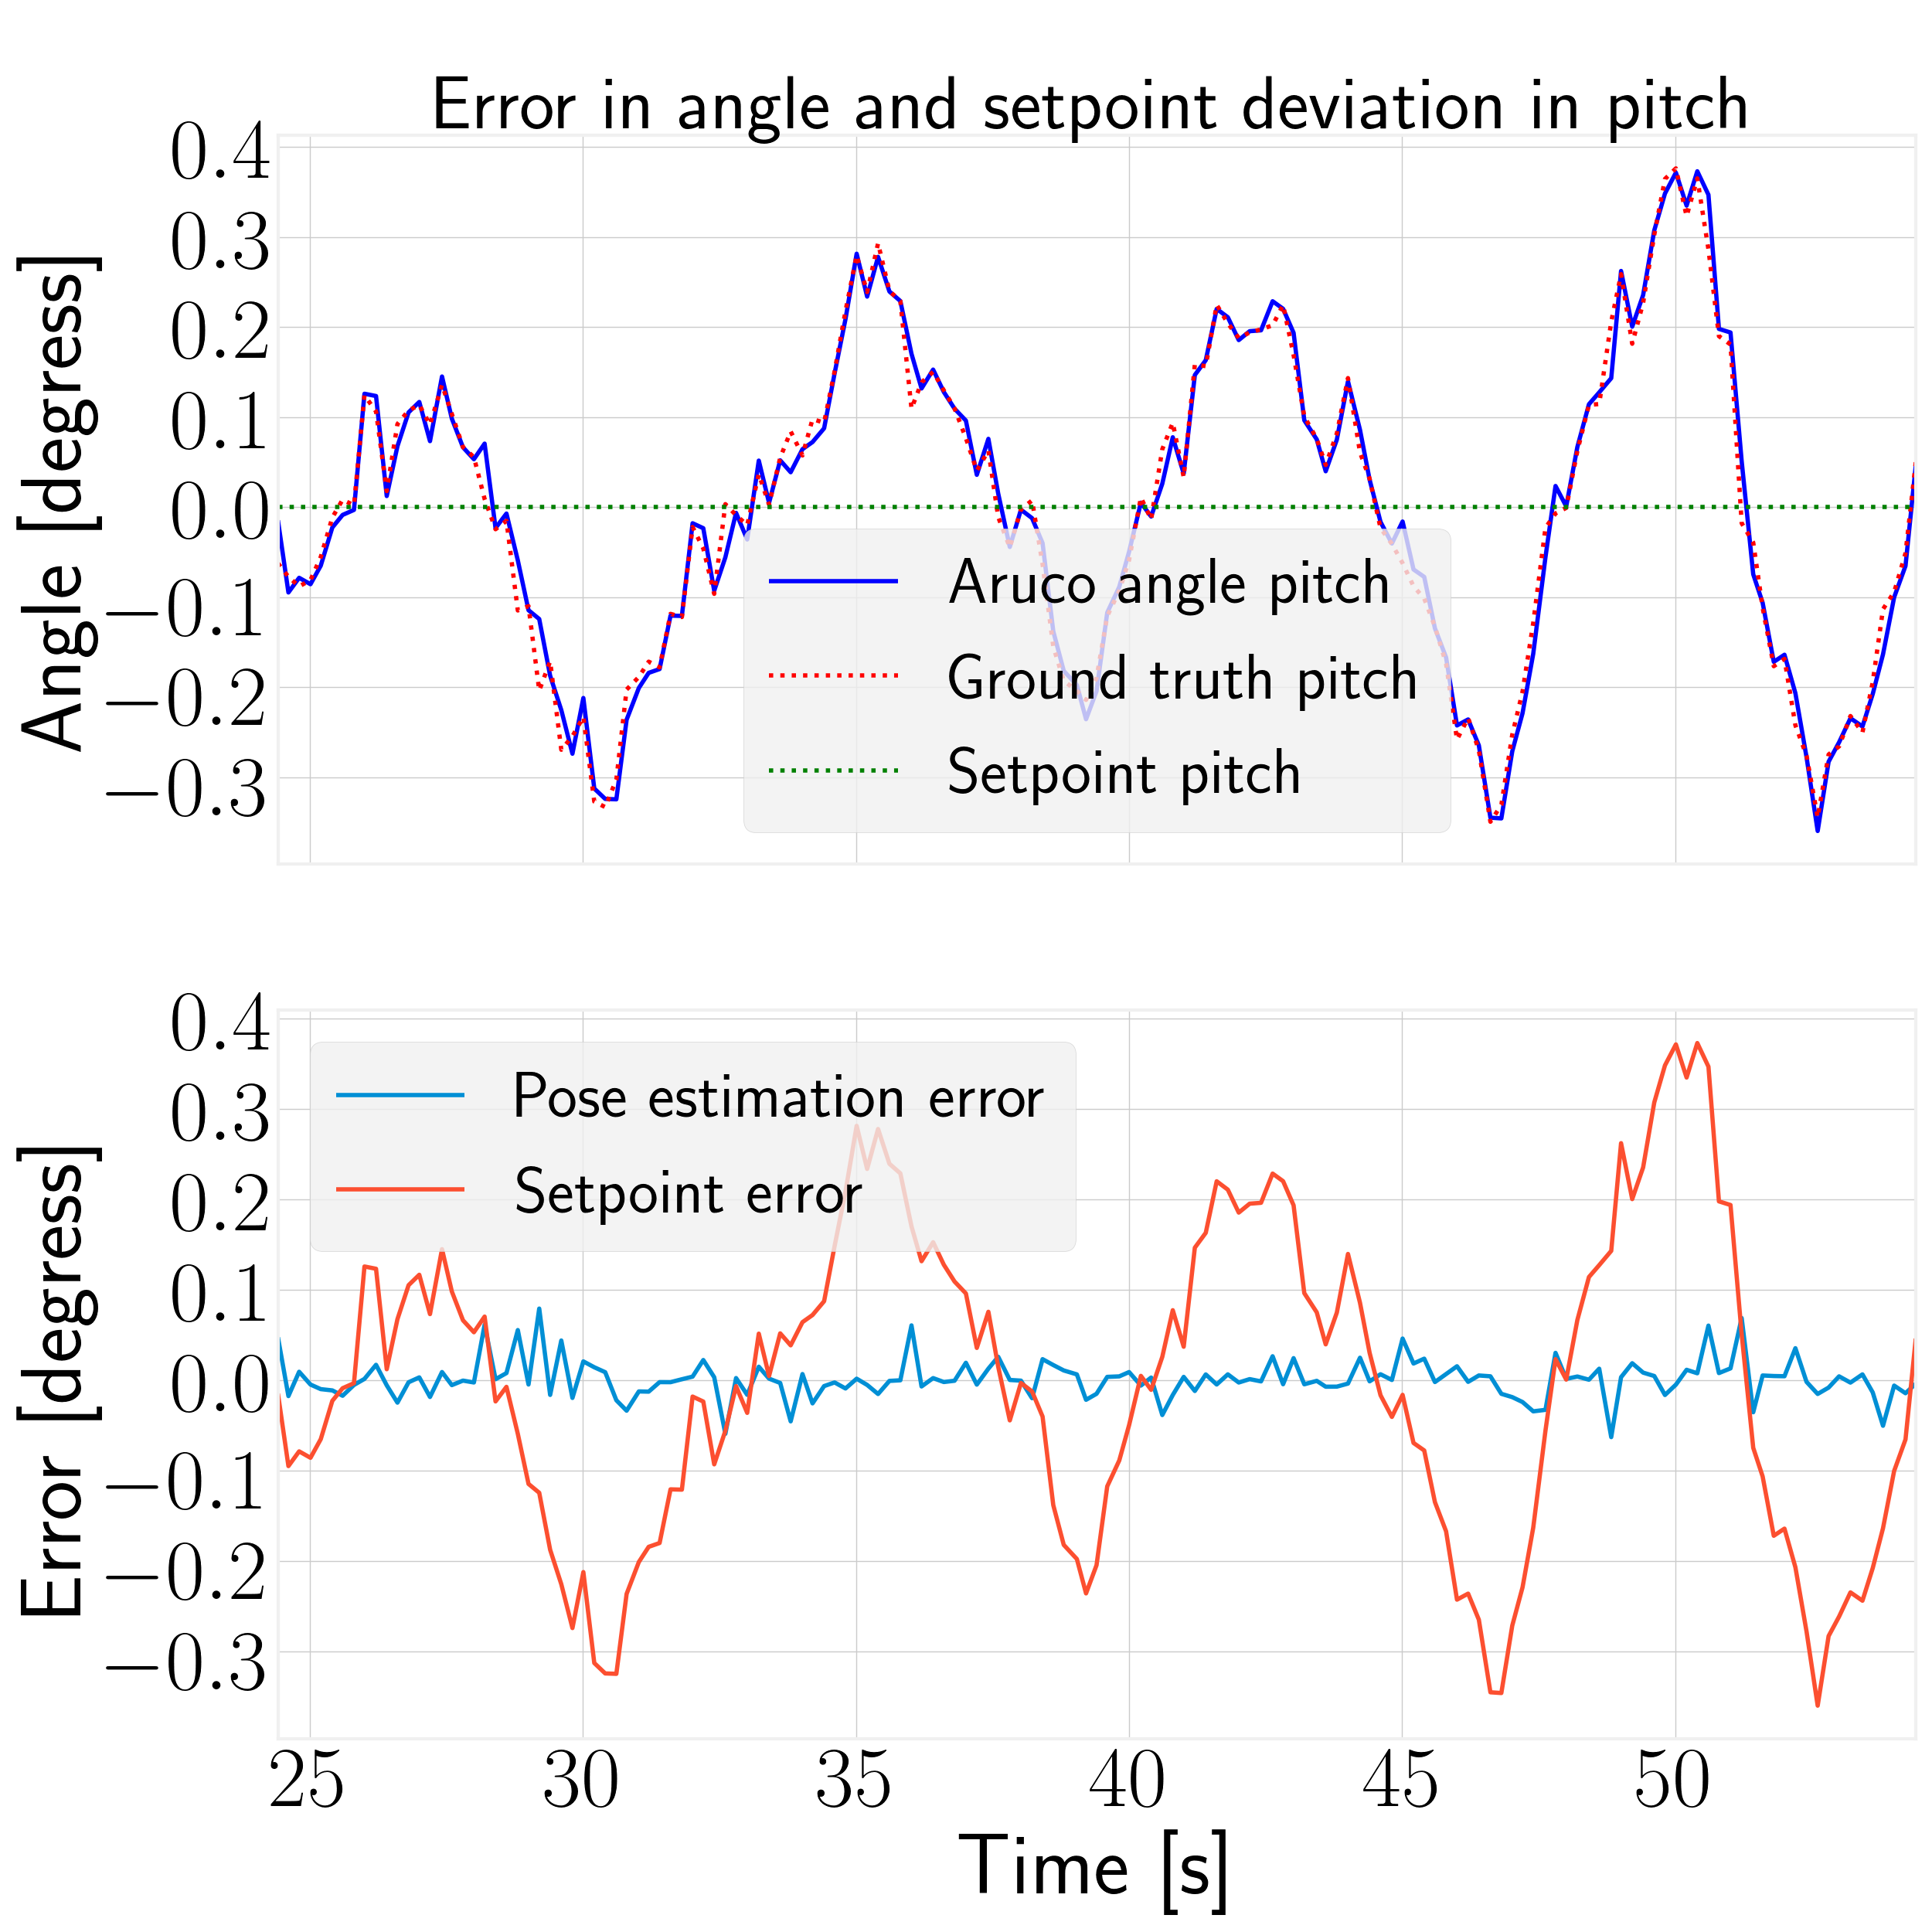
\includegraphics[width=\textwidth]{../Figures/hold_pose_using_aruco_pose_estimation/pose_error_pitch_test1.png}
        \caption{}
        \label{fig:hold_pose_estimation_test5_pitch}
    \end{subfigure}
     \hspace{0.2em}
    \begin{subfigure}[t]{.30\textwidth}
        \centering
        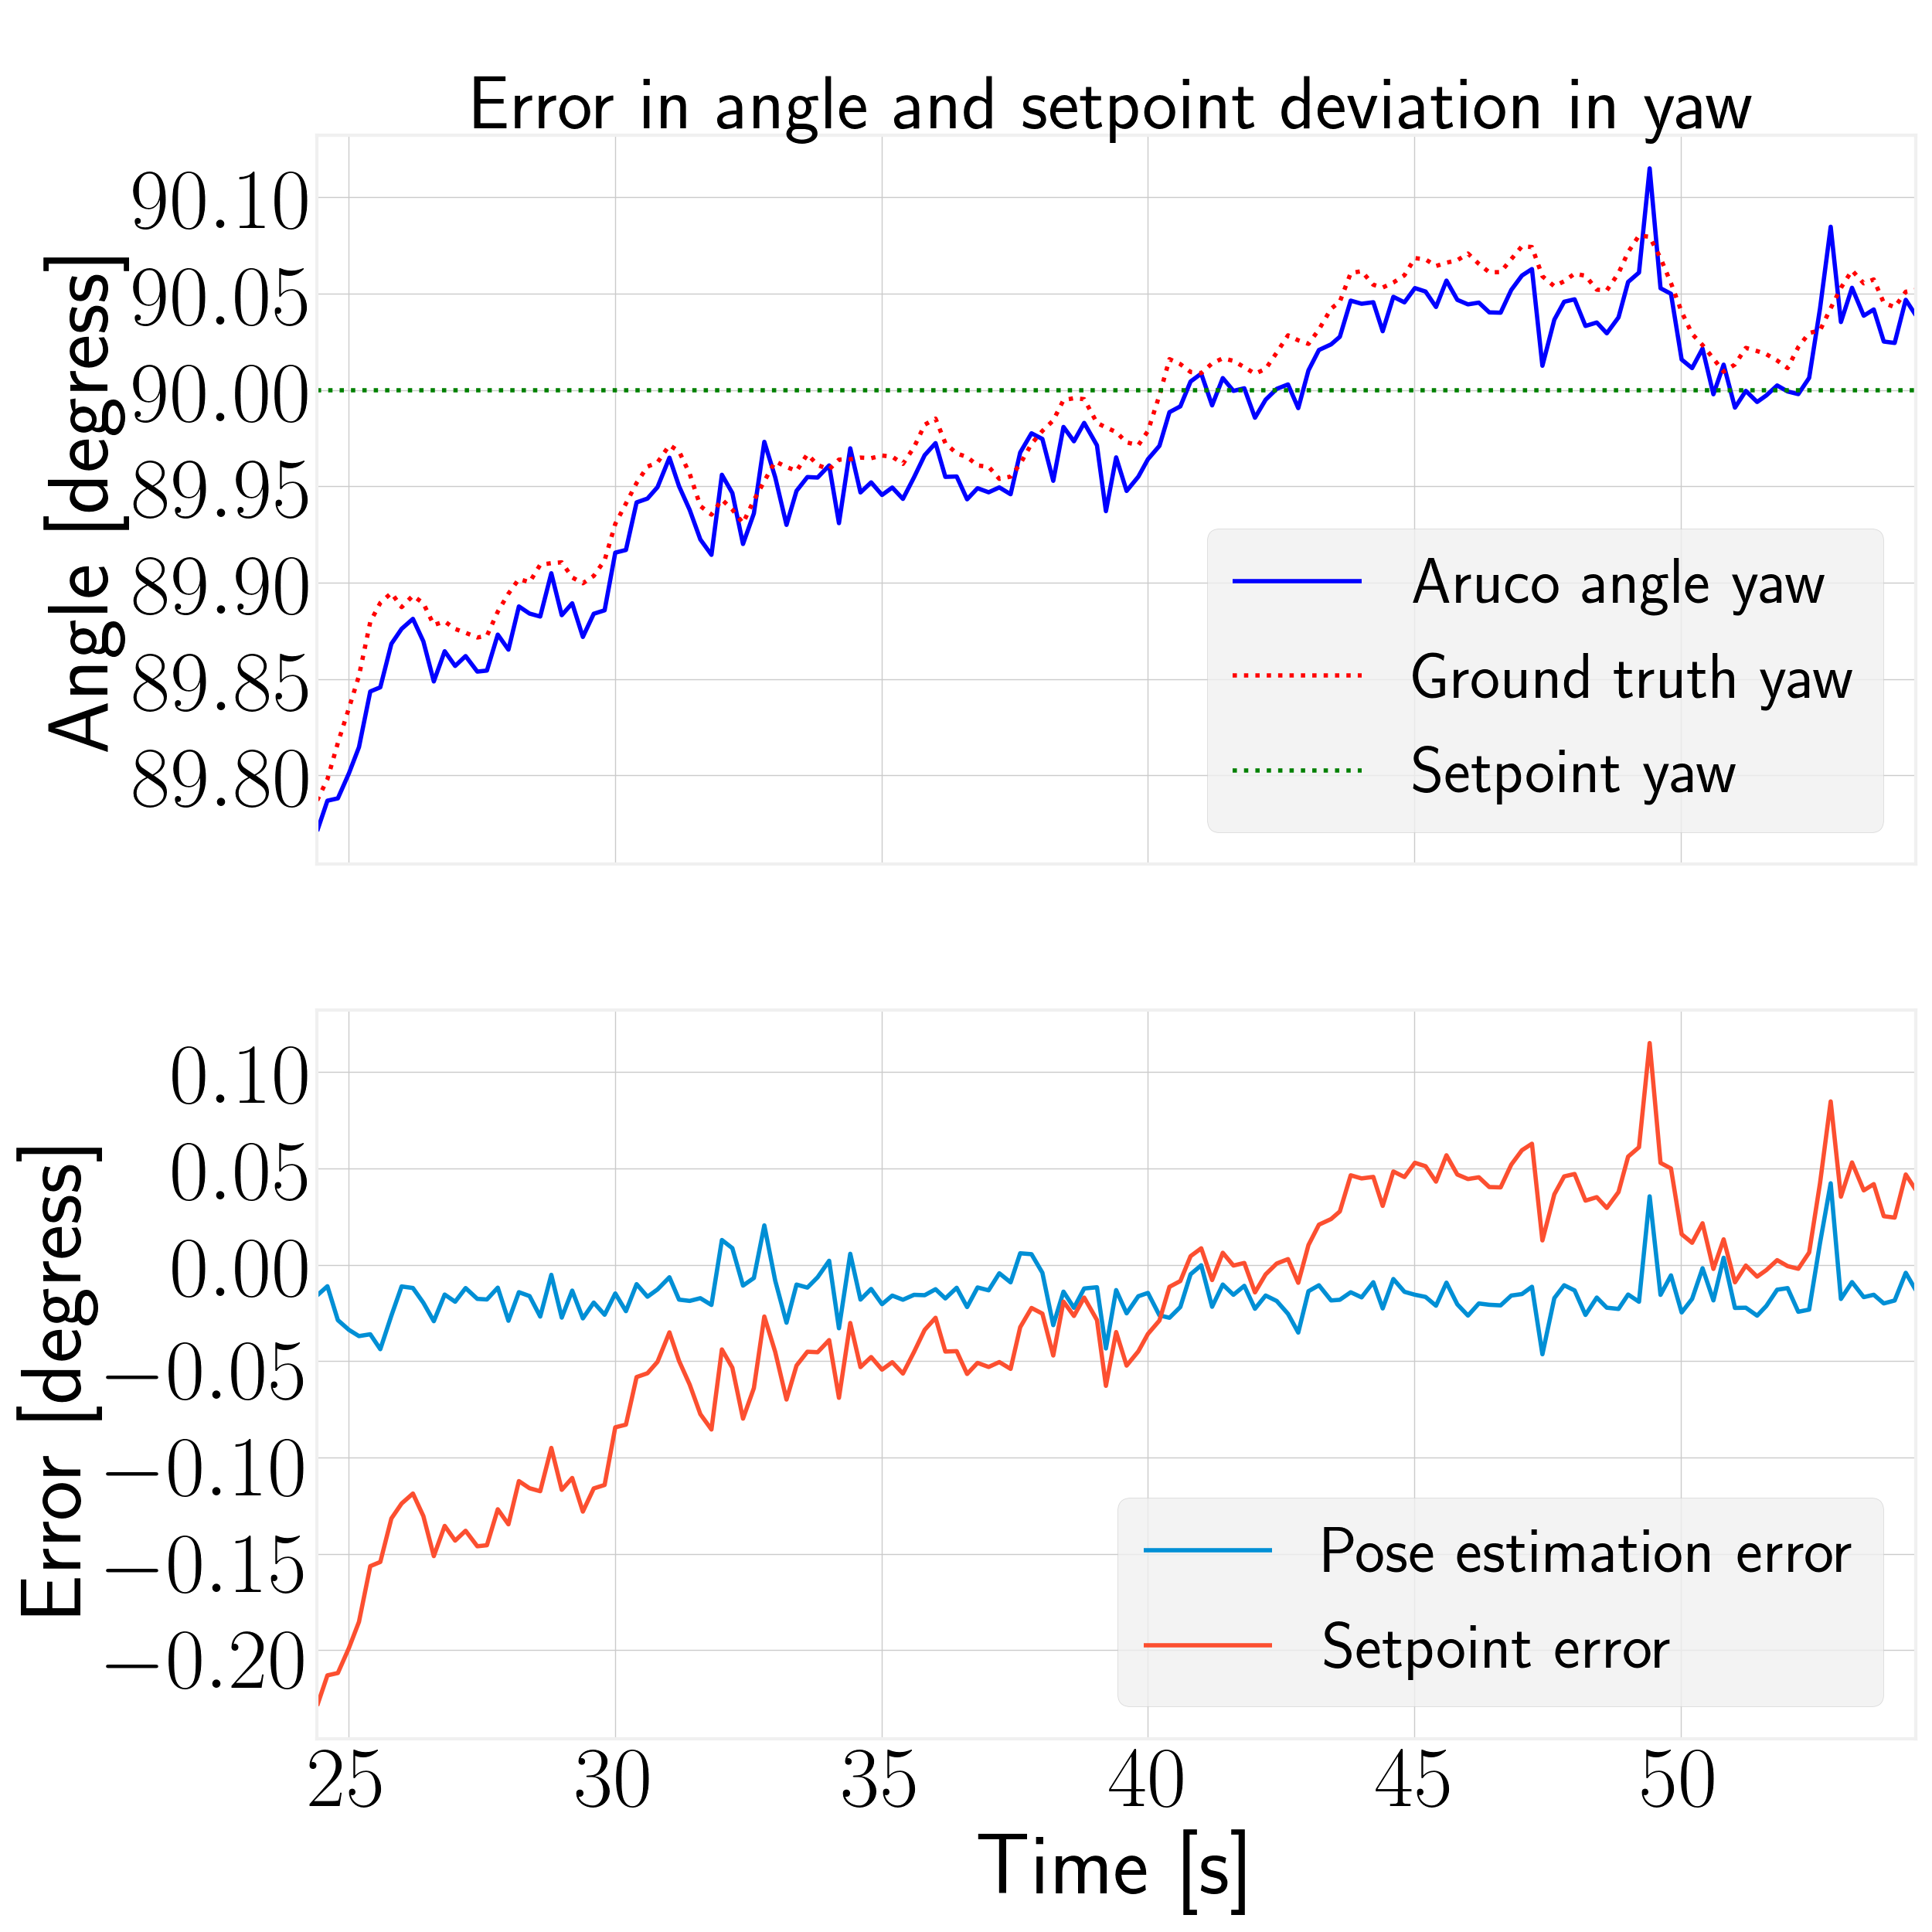
\includegraphics[width=\textwidth]{../Figures/hold_pose_using_aruco_pose_estimation/pose_error_yaw_test1.png}
        \caption{}
        \label{fig:hold_pose_estimation_test5_yaw}
    \end{subfigure}
    \caption{Illustration of the pose estimation and setpoint error using configuration in Figure \ref{fig:hold_pose_aruco_board_five}. The error in the angle estimations can be seen to be very small as well as the target setpoint which again confirms that operating close to the board decreases the pose estimation error}
    \label{fig:hold_pose_estimation_test5_error_angle}
\end{figure}

In order to replicate the tests, the command in Listing \ref{lst:hold_aruco_pose_test} can be run from the terminal.

\definecolor{lightgreen}{rgb}{0.56, 0.93, 0.56}
\definecolor{moonstoneblue}{rgb}{0.45, 0.66, 0.76}
\begin{listing}[H] 
\begin{tcolorbox}[
    enhanced,
    attach boxed title to top left={xshift=6mm,yshift=-3mm},
    colback=lightgreen!20,
    colframe=lightgreen,
    fonttitle=\bfseries\color{black},
]
\begin{minted}[ numbersep=6pt, linenos=true, breaklines=true, breakanywhere=true, mathescape, escapeinside=||,fontsize=\small]{bash}
#For execution of the giving test
roslaunch px4 gazebo_sim_v1.0.launch worlds:=optitrack_big_board_onepattern.world drone_control_args:="hold_aruco_pose_test" x:=-4.0 y:=0.0 headless:=false gui:=true
\end{minted}
\end{tcolorbox}
\caption{Command to be used to replicate the test}
\label{lst:hold_aruco_pose_test}    
\end{listing} 

Here the position for x and y is set to (3, 3.3), (3,0), (3,-3.3), (-4,0) and (-4,0) for the test in Figure \ref{fig:hold_pose_aruco_board_three}, \ref{fig:hold_pose_aruco_board_four}, \ref{fig:hold_pose_aruco_board_five}, \ref{fig:hold_pose_aruco_board_one_noWind} and \ref{fig:hold_pose_aruco_board_one_5-7ms_wind} respectively. The wind in the simulation can be activated by changing the followings lines in Listing \ref{lst:hold_aruco_pose_test_activate_wind} in the file /software/ros\_workspace/PX4-software/optitrack\_big\_board\_onepattern.world. All these values were initially set to zero to disable the use of wind. 

\definecolor{lightgreen}{rgb}{0.56, 0.93, 0.56}
\definecolor{moonstoneblue}{rgb}{0.45, 0.66, 0.76}
\begin{listing}[H] 
\begin{tcolorbox}[
    enhanced,
    attach boxed title to top left={xshift=6mm,yshift=-3mm},
    colback=lightgreen!20,
    colframe=lightgreen,
    fonttitle=\bfseries\color{black},
]
\begin{minted}[ numbersep=6pt, linenos=true, breaklines=true, breakanywhere=true, mathescape, escapeinside=||,fontsize=\small]{bash}
<plugin name='wind_plugin' filename='libgazebo_wind_plugin.so'>
  <frameId>base_link</frameId>
  <namespace>/foo/bar</namespace>
  <xyzOffset>0 0 0</xyzOffset>
  <windDirectionMean>1 1 1</windDirectionMean>
  <windDirectionVariance>0.05</windDirectionVariance>
  <windVelocityMean>1.0</windVelocityMean>
  <windVelocityVariance>0.05</windVelocityVariance>
  <windGustDirection>1 1 1</windGustDirection>
  <windPubTopic>world_wind</windPubTopic>
</plugin>
\end{minted}
\end{tcolorbox}
\caption{Activation of wind plugin for the \textit{optitrack\_big\_board\_onepattern.world} world}
\label{lst:hold_aruco_pose_test_activate_wind}    
\end{listing} 

\subsubsection{GPS to vision navigation}
\label{sec:gps2vision_transition}

The most important part of the simulations was the actual transitions between using GPS and vision as navigation. Because the influences of wind plays a major part of the stability of this transition, the simulated environment will include wind speeds between 5-7 $\frac{m}{s}$ and 7-10 $\frac{m}{s}$ for stress test of the system. This can be seen in Figure \ref{fig:gps2vision_states}. 

\begin{figure}[H]
    \centering
    \begin{subfigure}[t]{.30\textwidth}
        \centering
        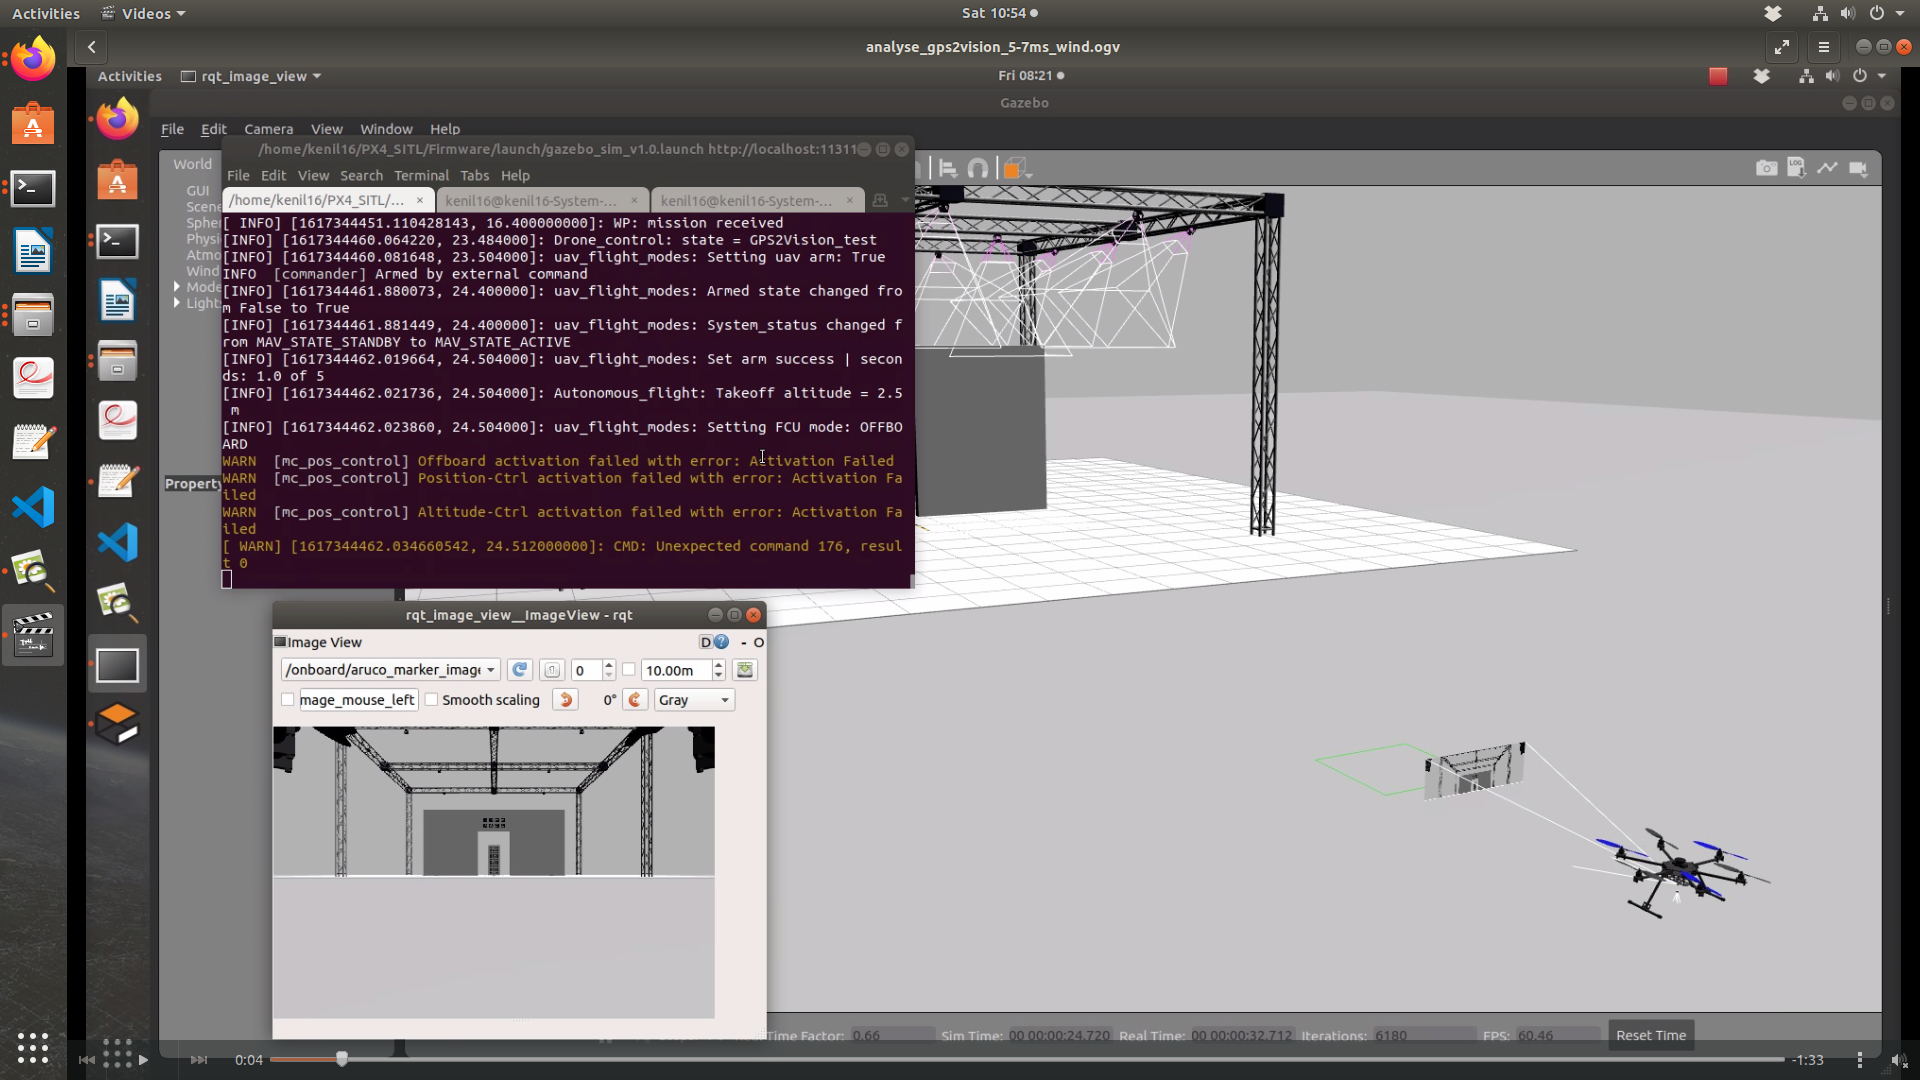
\includegraphics[width=\textwidth]{../Figures/GPS2Vision/drone_start_pose_gps.png}
        \caption{}
        \label{fig:gps2vision_gps}
    \end{subfigure}
     \hspace{0.2em}
    \begin{subfigure}[t]{.30\textwidth}
        \centering
        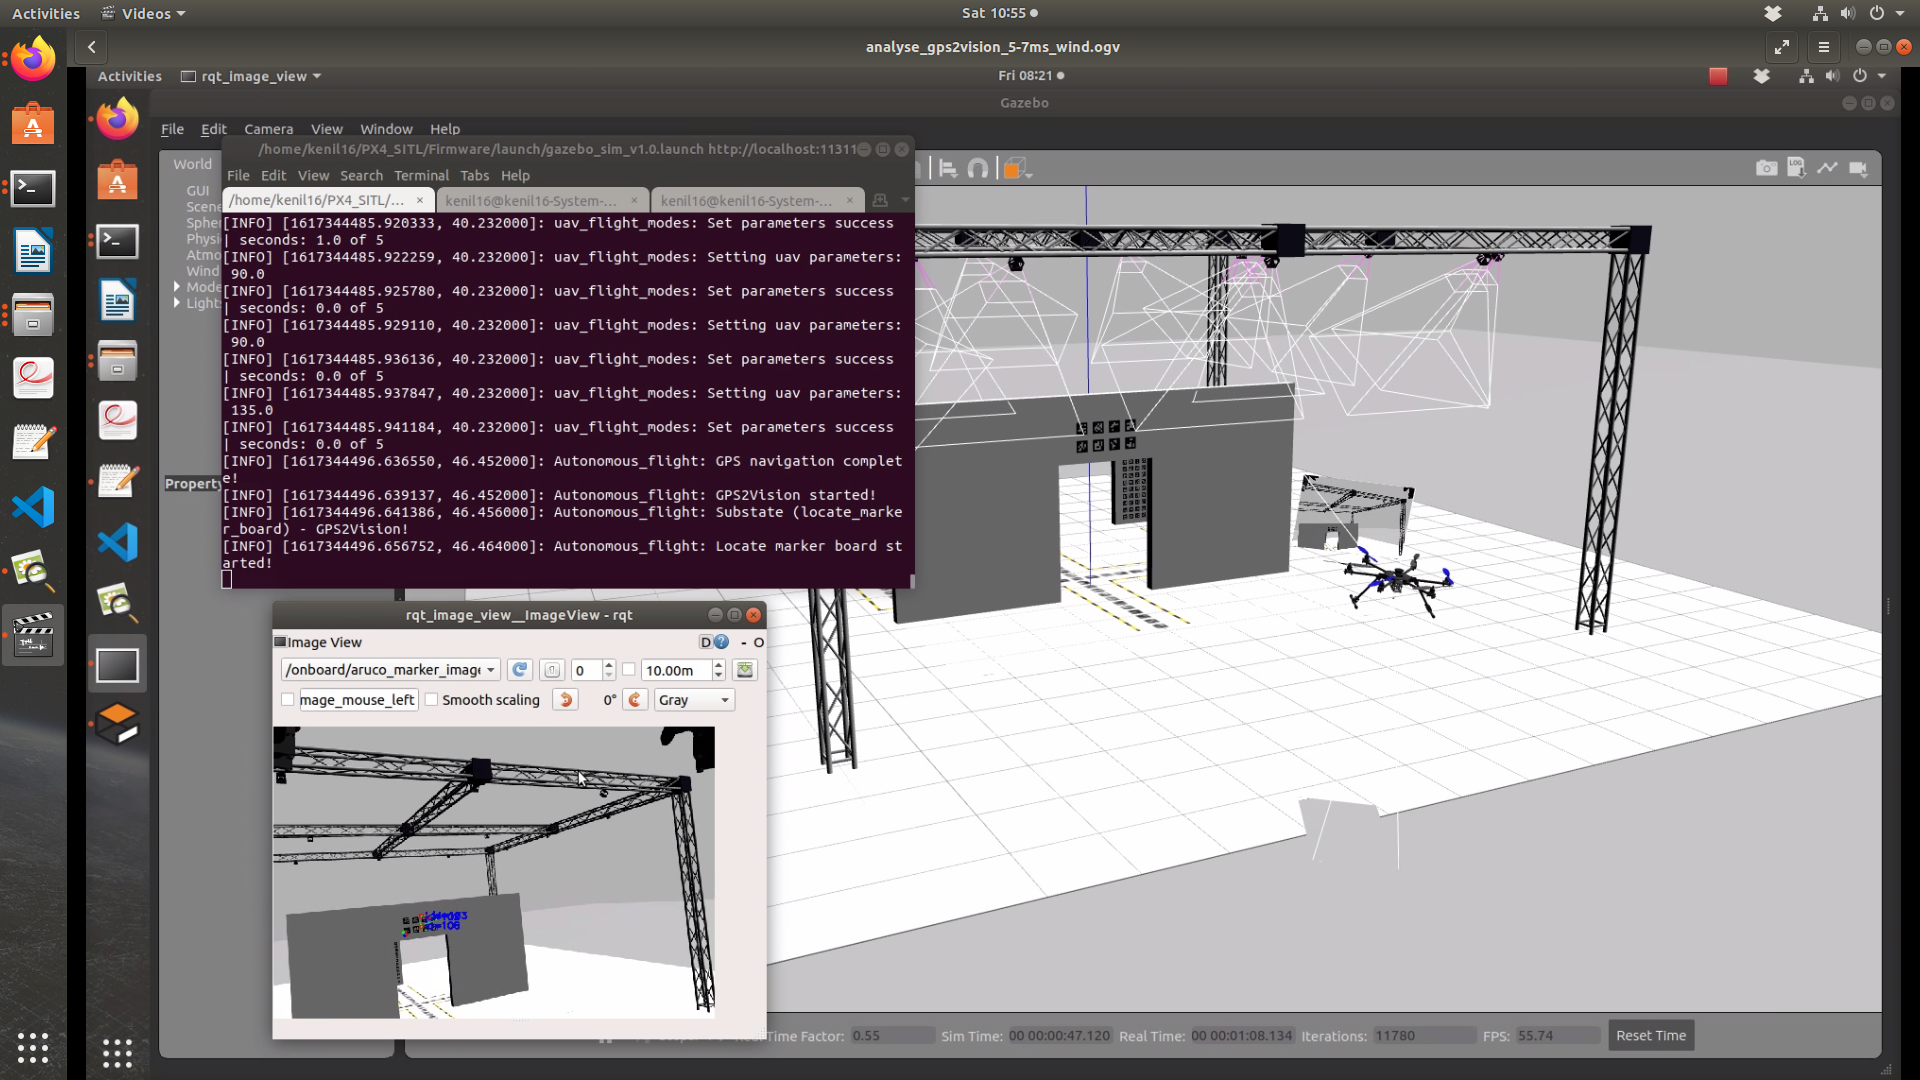
\includegraphics[width=\textwidth]{../Figures/GPS2Vision/drone_locate_board.png}
        \caption{}
        \label{fig:gps2vision_locate_board}
    \end{subfigure}
         \hspace{0.2em}
    \begin{subfigure}[t]{.30\textwidth}
        \centering
        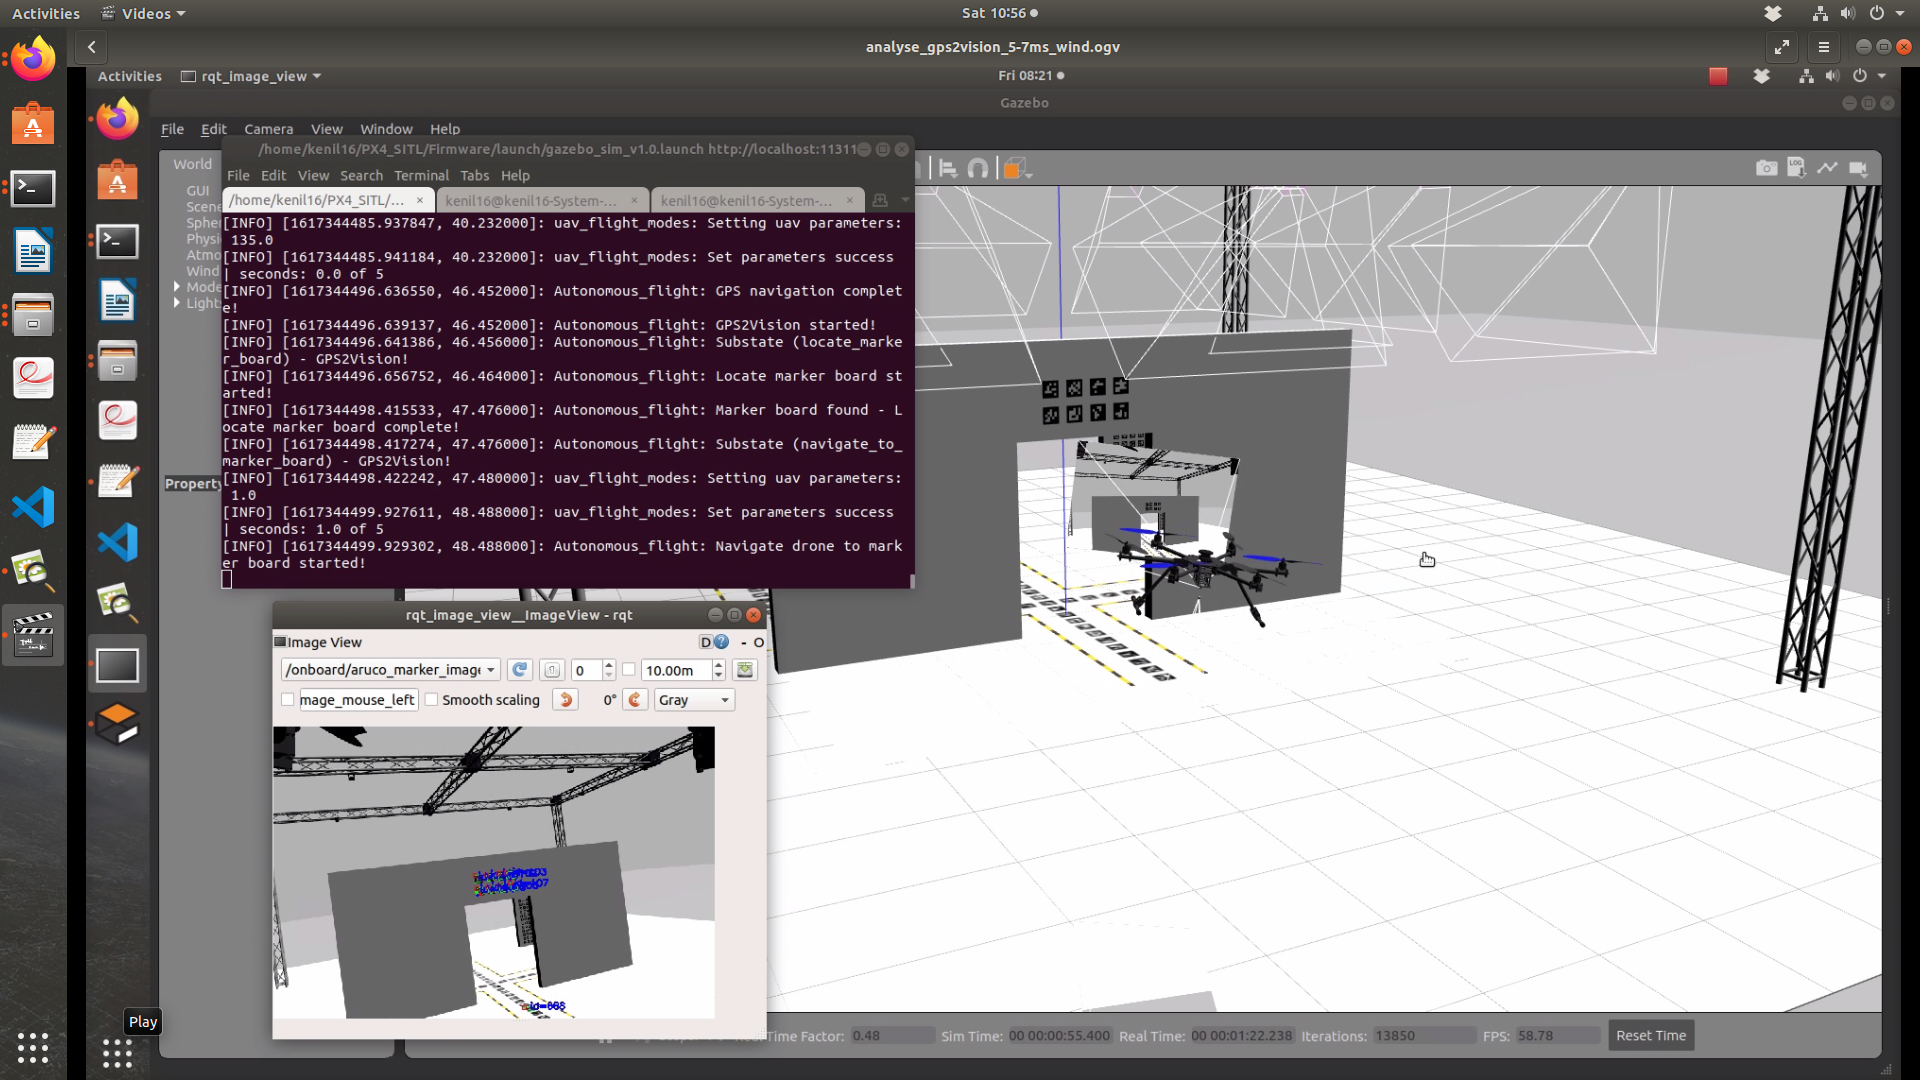
\includegraphics[width=\textwidth]{../Figures/GPS2Vision/drone_navigate_to_board.png}
        \caption{}
        \label{fig:gps2vision_navigate_to_board}
    \end{subfigure}
         \hspace{0.2em}
    \begin{subfigure}[t]{.30\textwidth}
        \centering
        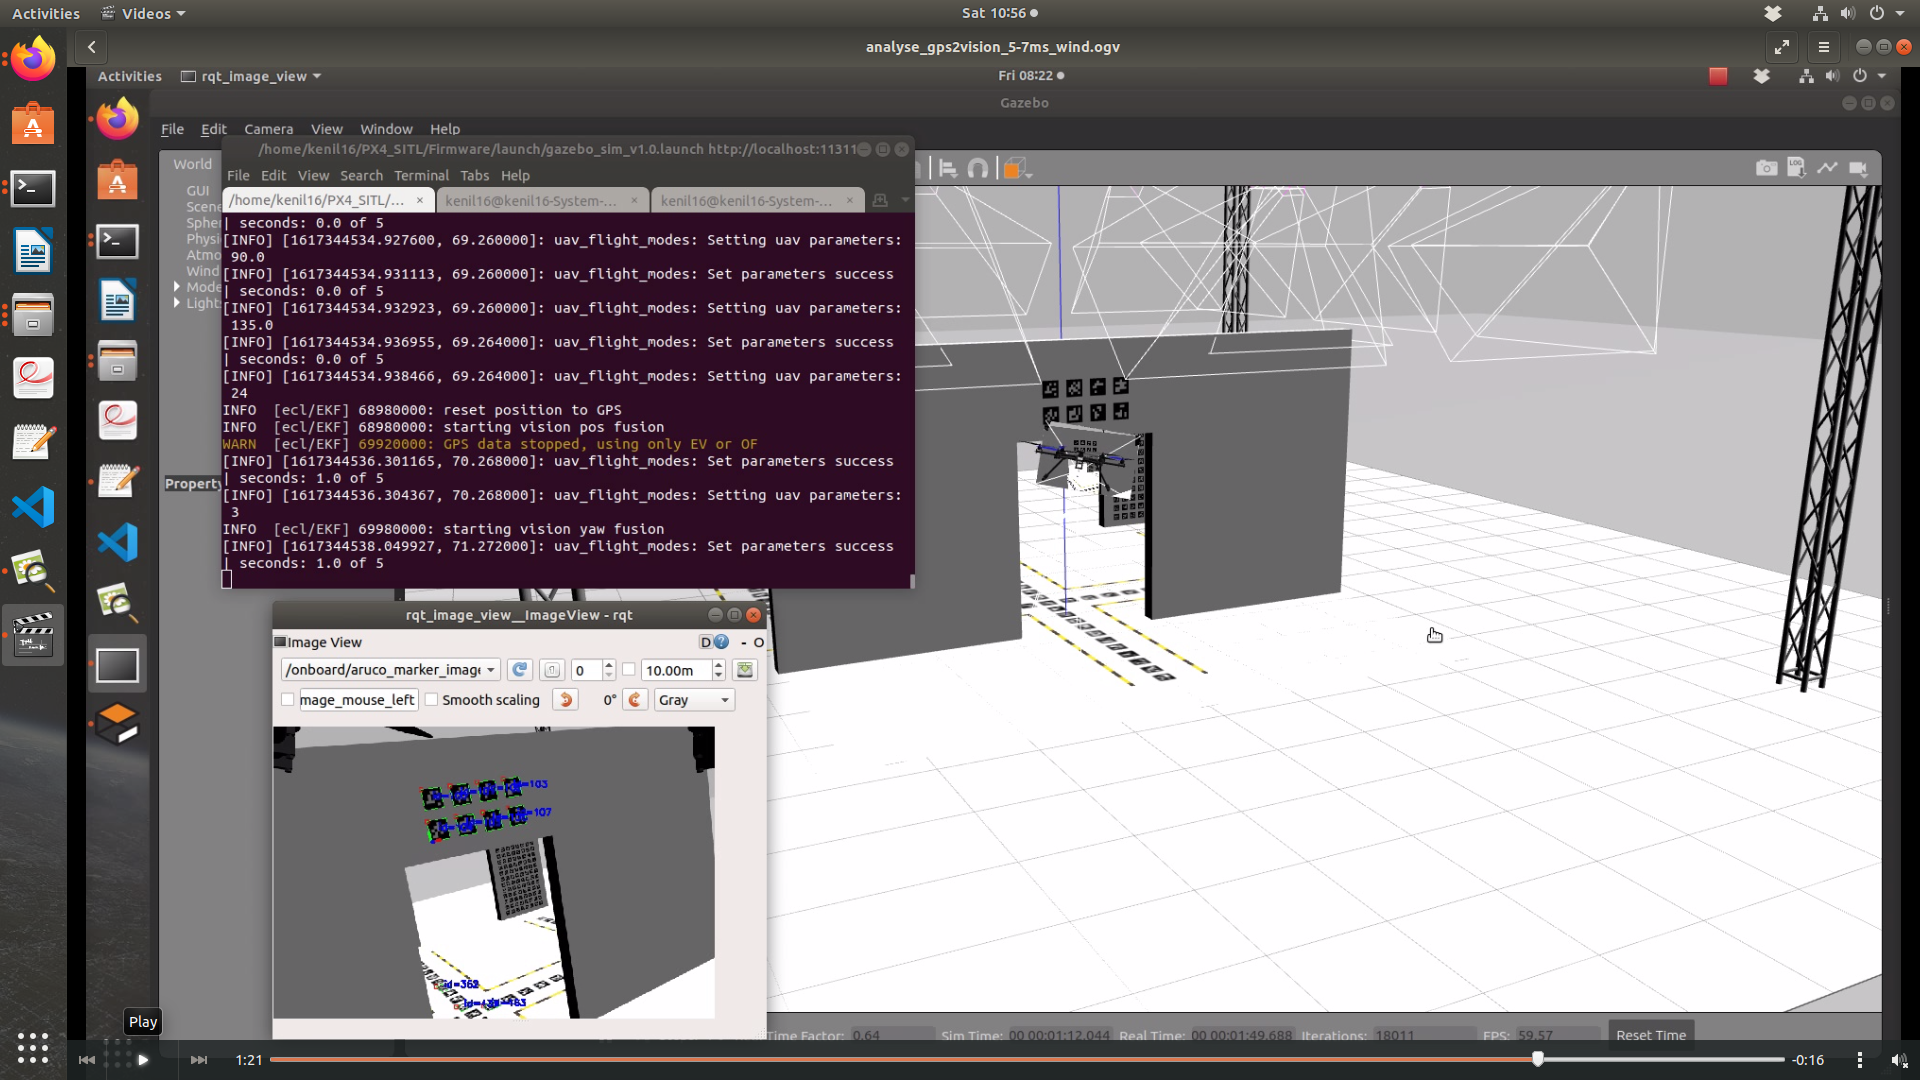
\includegraphics[width=\textwidth]{../Figures/GPS2Vision/drone_gps2vision_transition.png}
        \caption{}
        \label{fig:gps2vision_gps2vision_transition}
    \end{subfigure}
         \hspace{0.2em}
    \begin{subfigure}[t]{.30\textwidth}
        \centering
        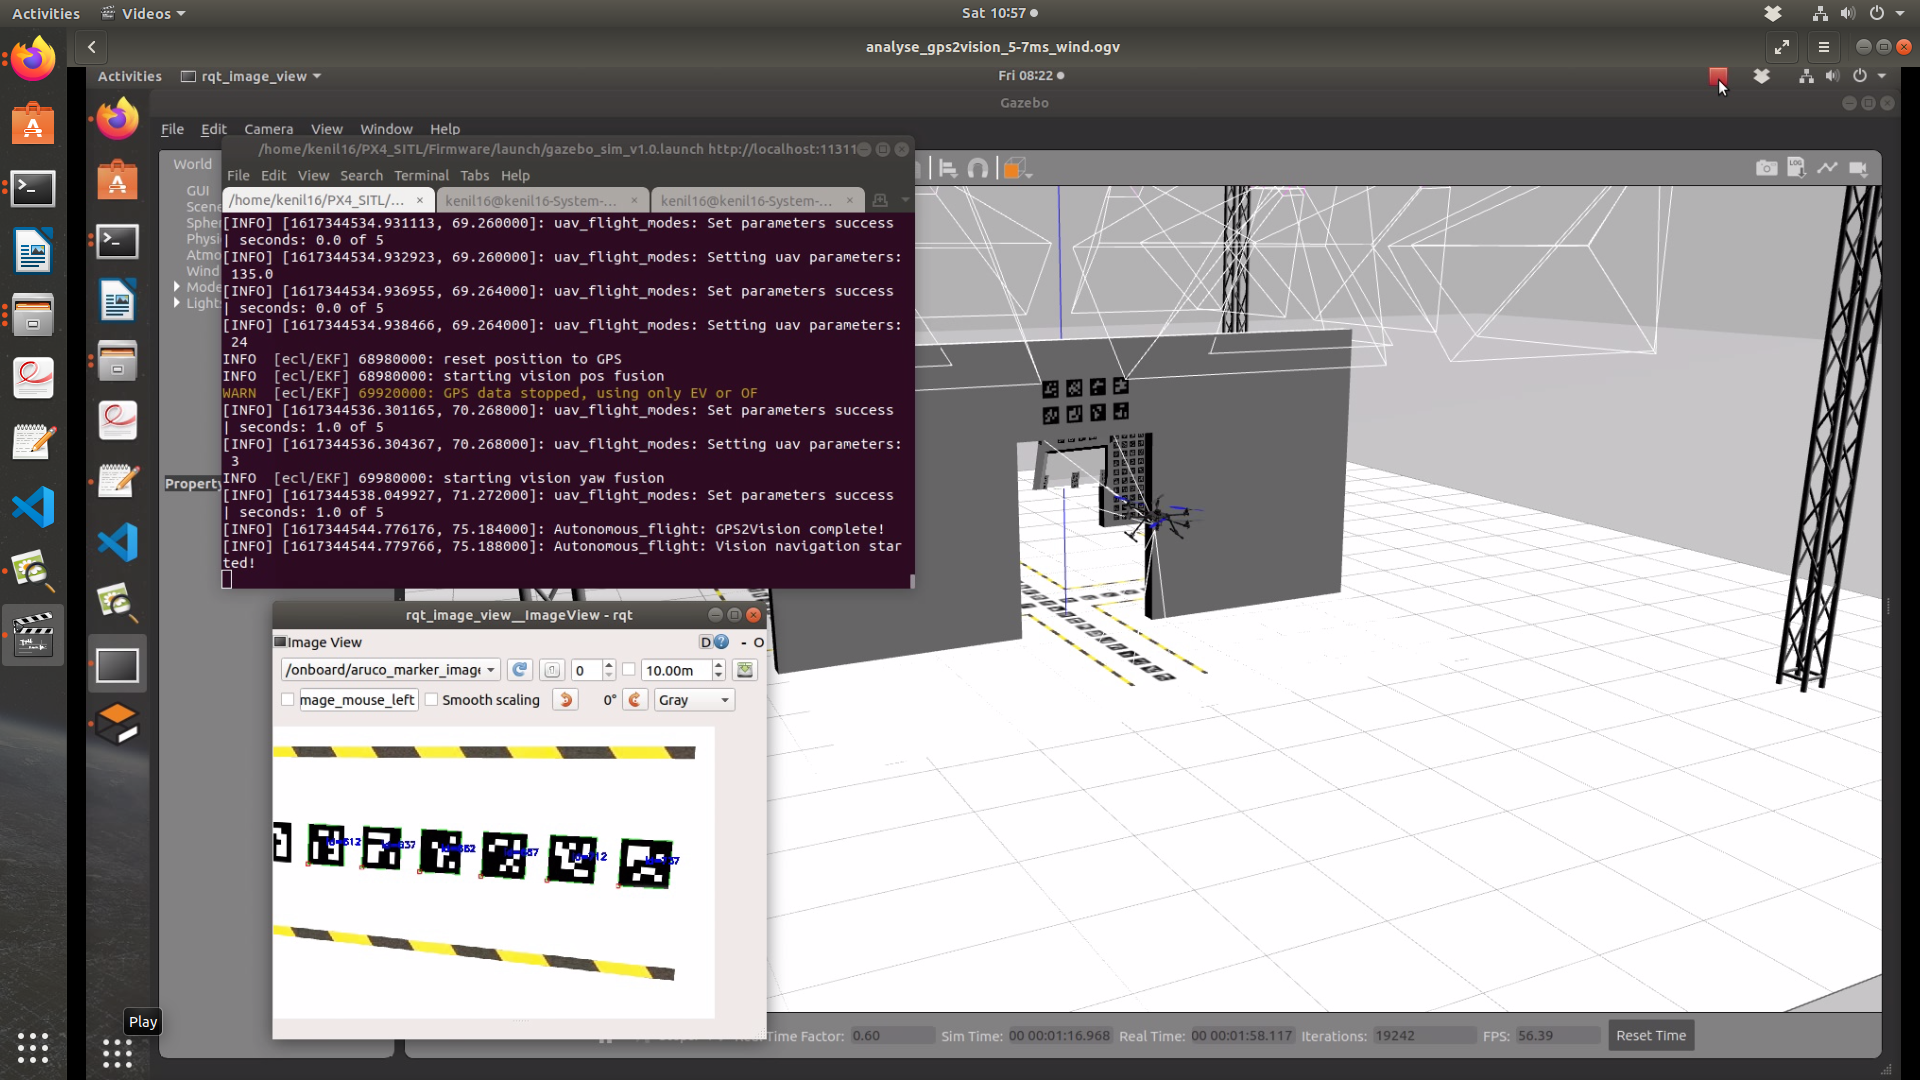
\includegraphics[width=\textwidth]{../Figures/GPS2Vision/drone_vision_navigation.png}
        \caption{}
        \label{fig:gps2vision_vision_navigation}
    \end{subfigure}
    \caption{Illustrations of the GPS2Vision test. Videos of the test can be seen on Github using \href{https://github.com/Kenil16/master_project/tree/master/test_videos/analyse_gps2vision_noWind}{GPS2Vision no wind}, \href{https://github.com/Kenil16/master_project/tree/master/test_videos/analyse_gps2vision_5-7ms_wind}{GPS2Vision 5-7 $\frac{m}{s}$ wind} and \href{https://github.com/Kenil16/master_project/tree/master/test_videos/analyse_gps2vision_7-10ms_wind}{GPS2Vision 7-10 $\frac{m}{s}$ wind}}
    \label{fig:gps2vision_states}
\end{figure}

\begin{table}[H]
    \centering
    \addtolength{\leftskip} {-2cm}
    \addtolength{\rightskip}{-2cm}
        \caption{Statistics of the results of the GPS2Vision tests. The GPS, locate board, navigate to board and GPS2Vision defines how much time the UAV in average spend in the different substates when executing the tests. It may be noticed that the UAV used a lot more time in GPS2Vision (gps to vision transition) in test 3. That it because the UAV had a hard time finding the ArUco markers located on the ground due to the angle in roll and pitch caused by the simulated wind. Moreover, it was only able to complete 17 out of 20 runs in test 3, because it lost sight of the ground marker in the gps to vision transition and had to land}
        \pgfplotstabletypeset[normal,
                columns/eg/.style={
                column name={Runs},
                dec sep align
        }
        ]{ %
       Wind & eg & Completed & Vel (GPS) & GPS & Locate board & Navigate to board & Vel (vision) & GPS2Vision\\
        \topmidheader{10}{\textbf{Test 1}}
          0 $\frac{m}{s}$ & 20 & 20 & $2\frac{m}{s}$ & $7.45s$ & $0.50s$ & $14.64s$ & $1\frac{m}{s}$ & $5.28s$\\
          \midheader{10}{\textbf{Test 2}}
               5-7 $\frac{m}{s}$ & 20 & 20 & $2 \frac{m}{s}$ & $6.66s$ & $1.76s$ & $16.05s$ & 1$\frac{m}{s}$ & $5.32s$\\
                  \midheader{10}{\textbf{Test 3}}
               7-10 $\frac{m}{s}$ & 20 & 17 & $2\frac{m}{s}$ & $7.04s$ & $3.71s$ & $16.24s$ & $1\frac{m}{s}$& $20.39s$\\
}
\label{tab:gps2vision_statistics}
\end{table}

\begin{figure}[H]
    \centering
    \begin{subfigure}[t]{.45\textwidth}
        \centering
        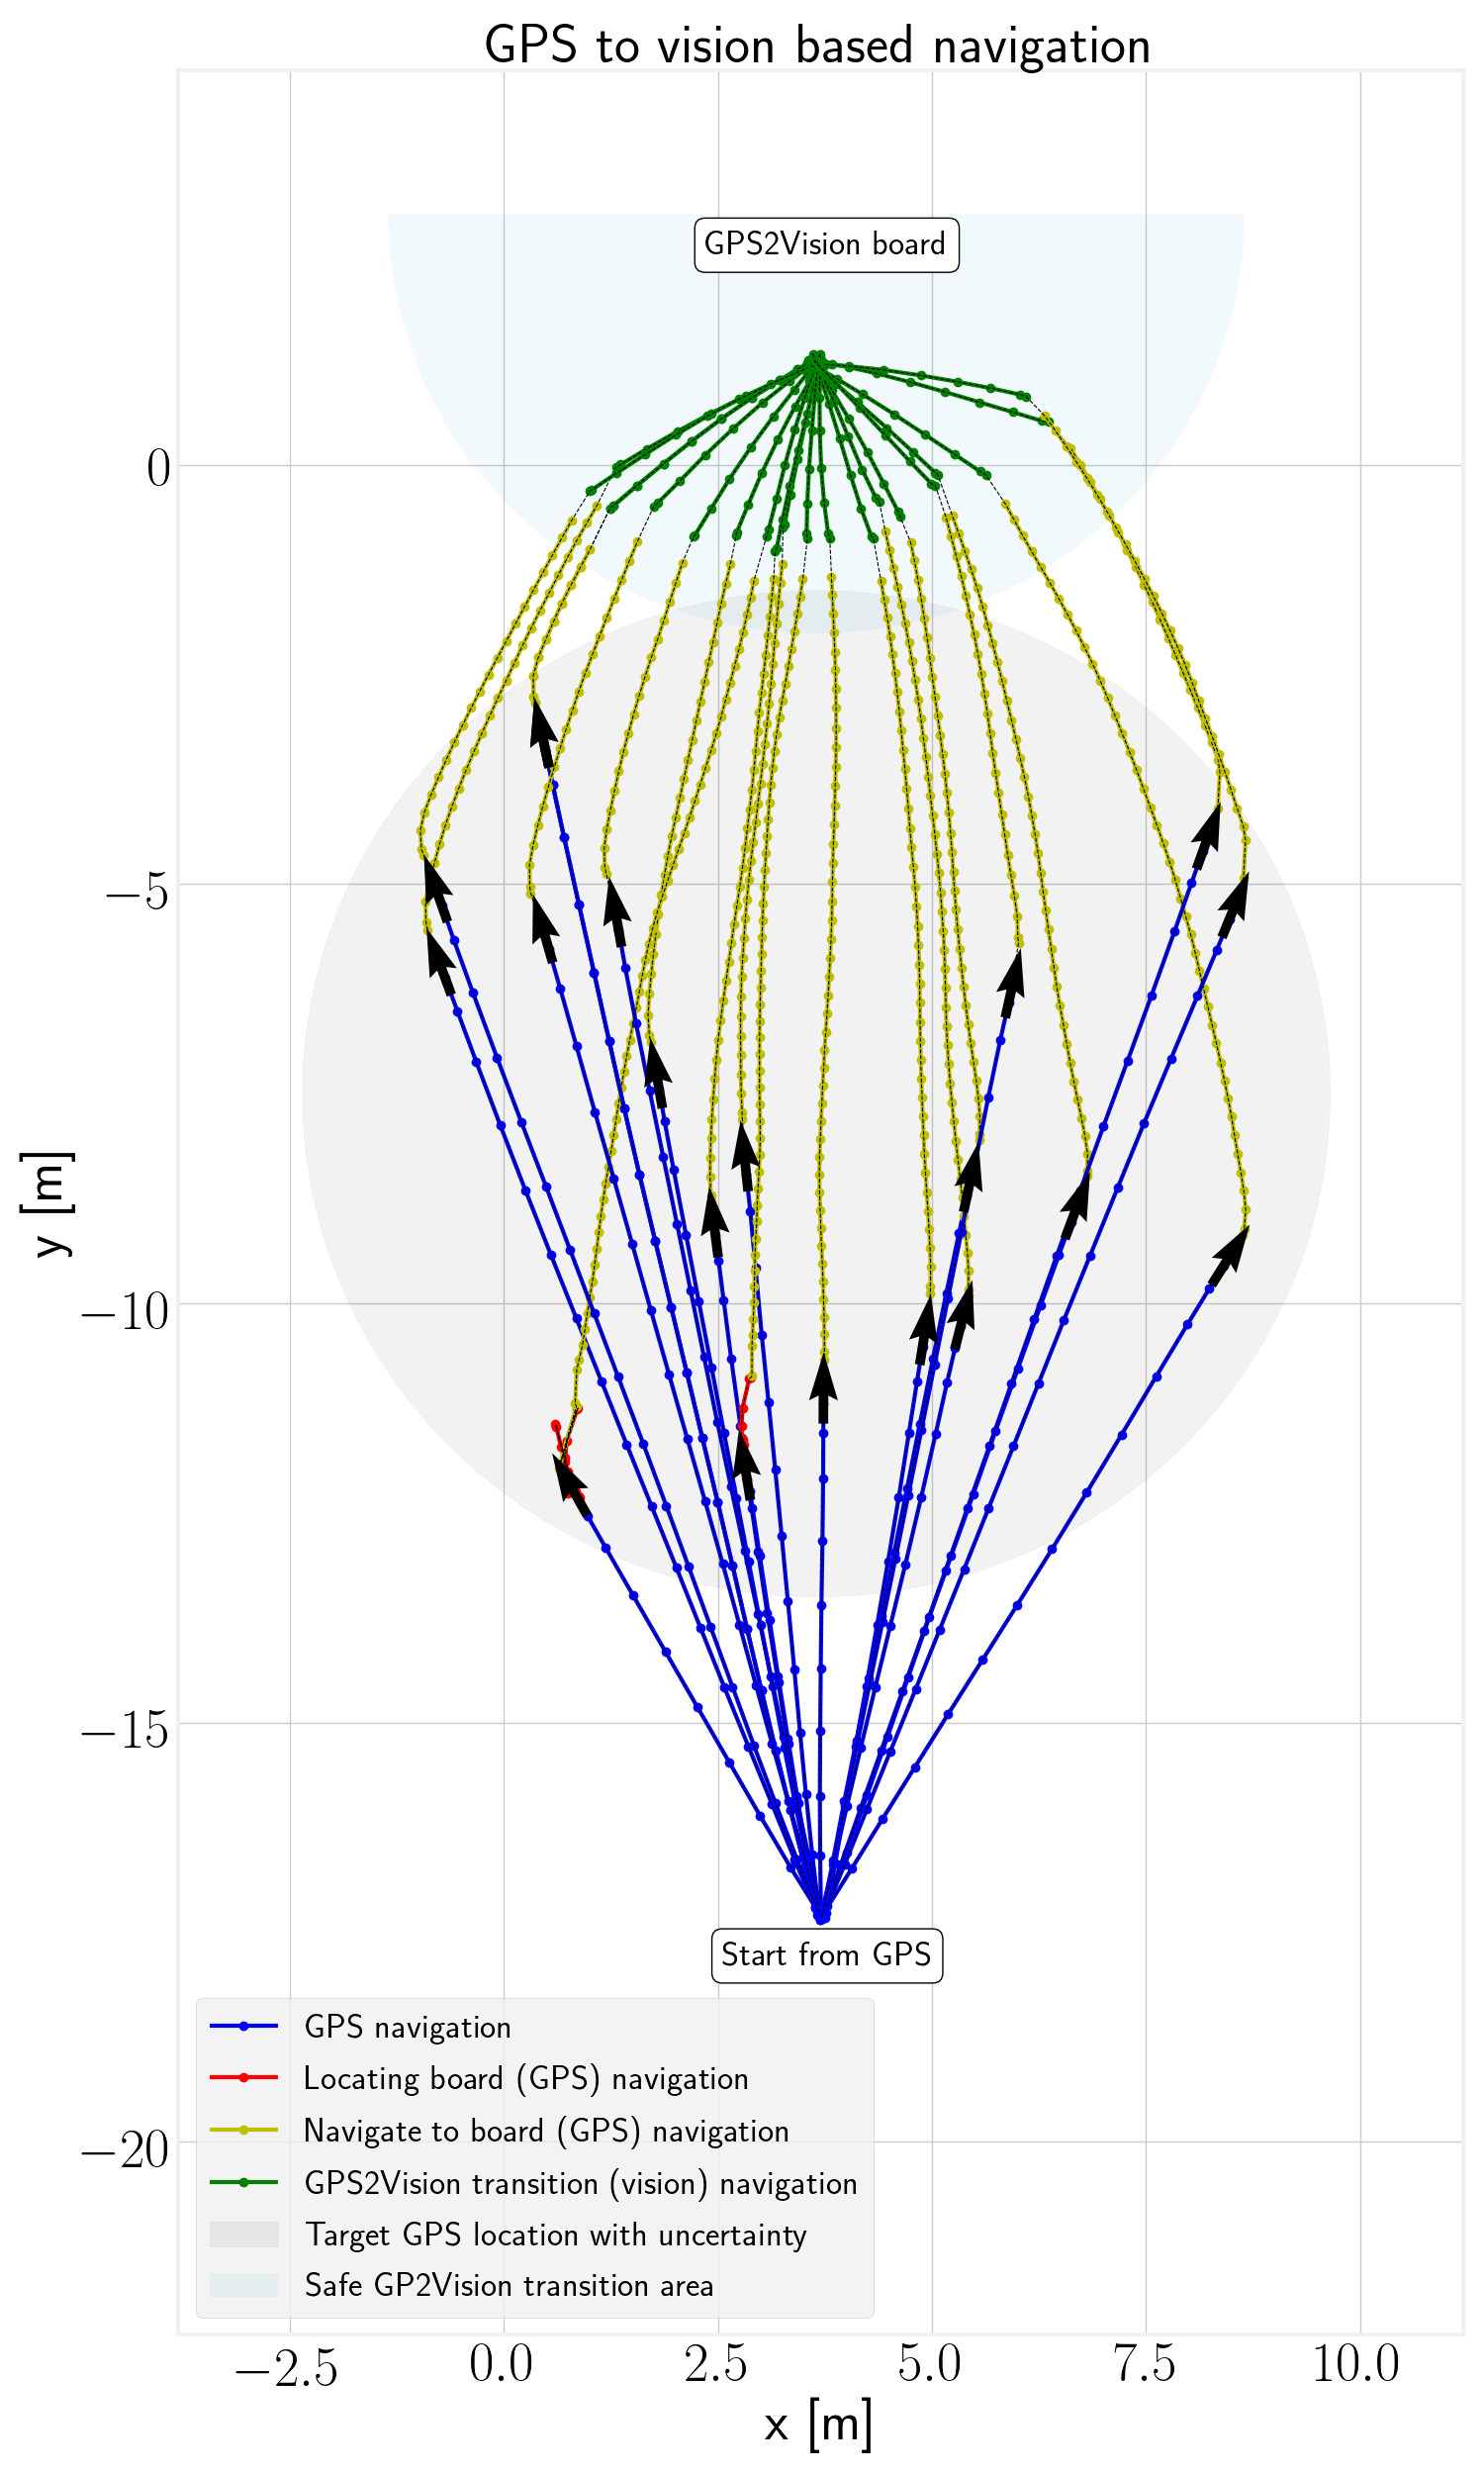
\includegraphics[width=\textwidth]{../Figures/GPS2Vision/test1_noWind_20_runs/gps2vision.png}
        \caption{}
        \label{fig:GPS2Vision_test1}
    \end{subfigure}
     \hspace{0.2em}
    \begin{subfigure}[t]{.45\textwidth}
        \centering
        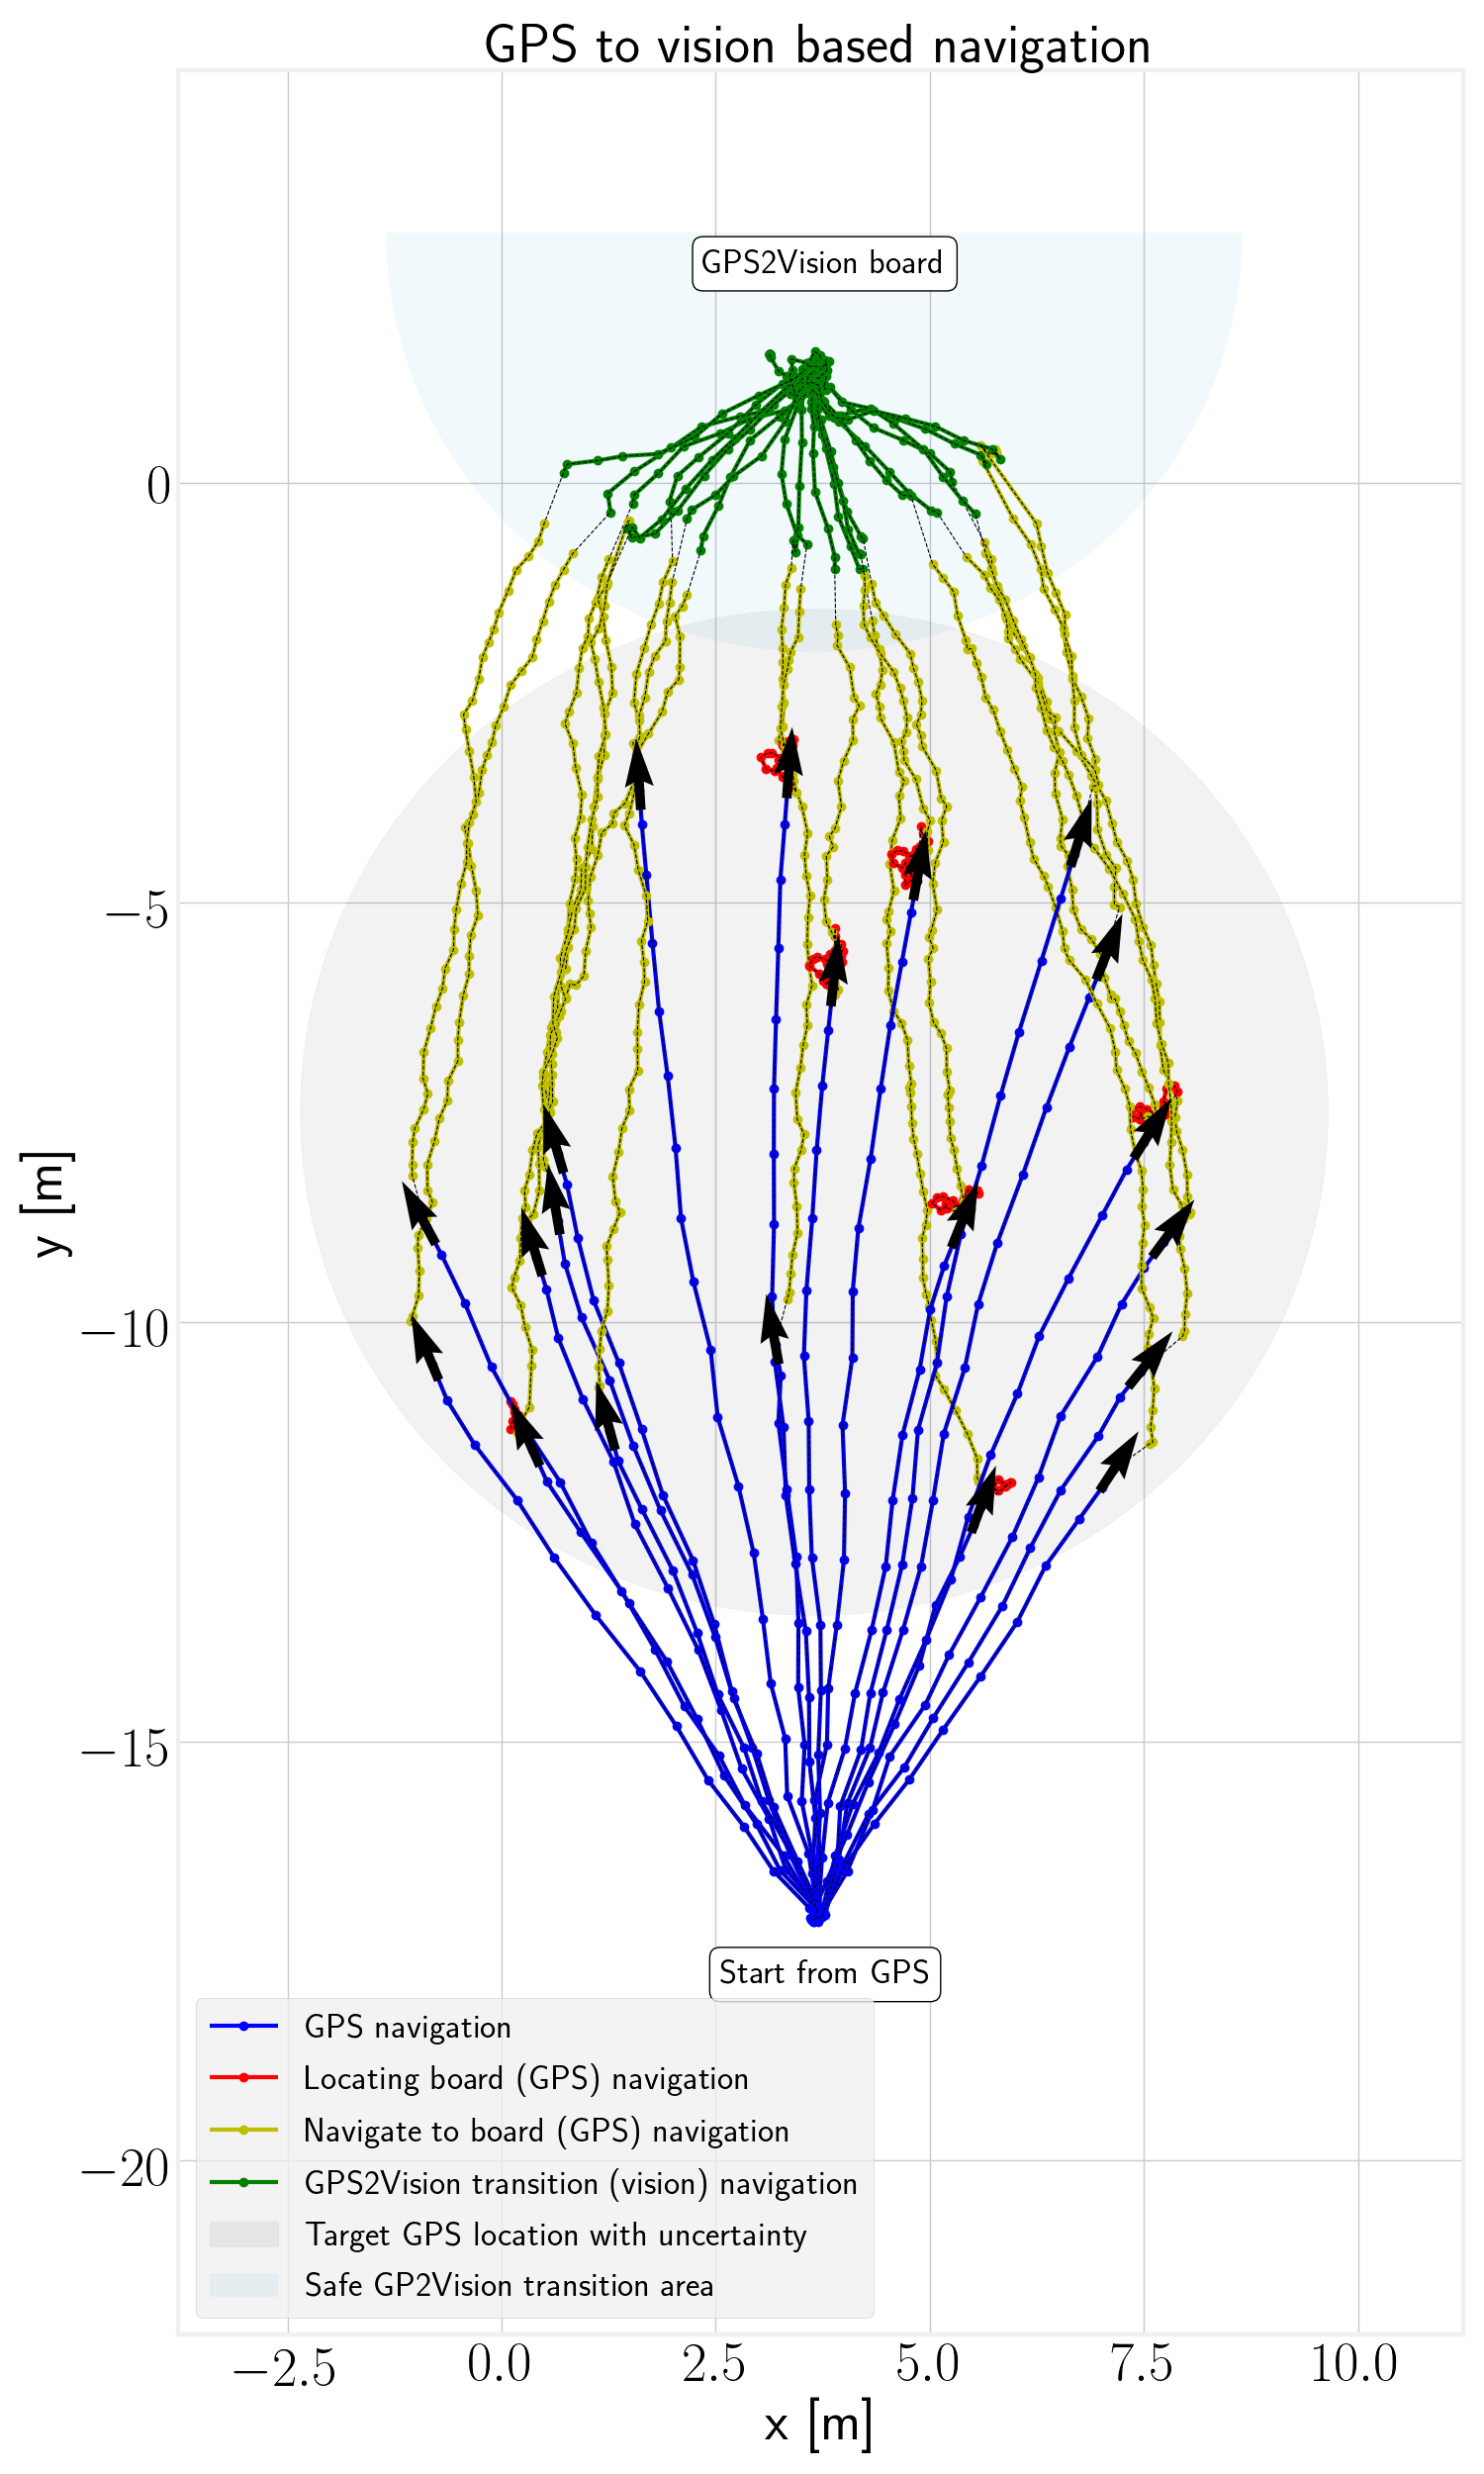
\includegraphics[width=\textwidth]{../Figures/GPS2Vision/test3_7-10ms_wind_20_runs/gps2vision.png}
        \caption{}
        \label{fig:GPS2Vision_test3}
    \end{subfigure}
    \caption{Illustrations of test 1 in Figure\ref{fig:GPS2Vision_test1} and test 3 in Figure \ref{fig:GPS2Vision_test3} summarized in Table \ref{tab:gps2vision_statistics}. The black arrows define the directions of movement of the UAV for each run along with ended GPS target location due to variations of $\pm 6$ meters in the GPS accuracy to take into account real life conditions. The actual target GPS location is predefined to be centered in the gray circle}
    \label{fig:GPS2Vision_test1_test3}
\end{figure}

In Figure \ref{fig:gps2vision_gps}, the UAV starts from an initial pose and moves to a predefined GPS target location. In Figure \ref{fig:gps2vision_locate_board}, the UAV has reached the target GPS location and begins to search for the GPS2Vision board. When the UAV has found the GPS2Vision board, it begins to navigate to it still using GPS as seen in Figure \ref{fig:gps2vision_navigate_to_board}. When the UAV is of a radius of maximum 5 meters away from the GPS2Vision board and the estimated pose is stable, it makes a GPS2Vision transition as seen in Figure \ref{fig:gps2vision_gps2vision_transition}. When the last setpoint is reached, the UAV now uses the bottom camera to enable the actual vision navigation which can be seen in Figure \ref{fig:gps2vision_vision_navigation}. 

In Figure \ref{fig:GPS2Vision_test1_test3}, a total of forty runs were performed with no wind in Figure \ref{fig:GPS2Vision_test1} and 7-10 $\frac{m}{s}$ simulated wind speeds in \ref{fig:GPS2Vision_test3}. The dots between the lines defines the actual point of ground truth measurement of the position of the UAV. The blue, red and yellow lines defines the use of GPS as pose estimate for navigation while the green lines defines the use of the GPS2Vision board as pose estimate. As it can be seen, the
transition of using vision instead of GPS first happens when the UAV is located inside of the \textit{safe transition area} visualized with a sky blue color. 

In order to replicate the tests, the command in Listing \ref{lst:GPS2Vision_test} can be run from the terminal.

\definecolor{lightgreen}{rgb}{0.56, 0.93, 0.56}
\definecolor{moonstoneblue}{rgb}{0.45, 0.66, 0.76}
\begin{listing}[H] 
\begin{tcolorbox}[
    enhanced,
    attach boxed title to top left={xshift=6mm,yshift=-3mm},
    colback=lightgreen!20,
    colframe=lightgreen,
    fonttitle=\bfseries\color{black},
]
\begin{minted}[ numbersep=6pt, linenos=true, breaklines=true, breakanywhere=true, mathescape, escapeinside=||,fontsize=\small]{bash}
#For execution of the giving test
roslaunch px4 gazebo_sim_v1.0.launch worlds:=optitrack_big_board_onepattern.world drone_control_args:="GPS2Vision_test" x:=-21.0 y:=0.0 headless:=false gui:=true
\end{minted}
\end{tcolorbox}
\caption{Command to be used to replicate the test}
\label{lst:GPS2Vision_test}    
\end{listing} 

For activating wind Listing \ref{lst:hold_aruco_pose_test_activate_wind} must be set. However, in the same piece of code the \textit{windVelocityMean} is set to 1.0 and 1.5 for test 1 and test 2 which insures wind speeds on approximately $5-7 \frac{m}{s}$ and $7-10 \frac{m}{s}$ respectively 

\subsubsection{Vision based navigation}
\label{sec:vision_based_navigation}

To analyze how the system performs when markers are not always visible in the image, a setup of different ArUco boards located on the ground has been proposed which can be seen in Figure \ref{fig:vision_navigation_boards}. This is done to stress test the system and evaluate the performance using the implemented sensor fusion. The UAV is set to move from a predefined location, to one of the landing stations and then back again. This can be seen in Figure \ref{fig:vision_navigation}. 

The ground truth pose of the UAV will be compared to the estimates of the pose from sensor fusion which is summarized in Table \ref{tab:vision_navigation_stastitics}. The waypoint error defined in Table \ref{tab:vision_navigation_stastitics}, means the maximum allowed error between the target setpoint and the estimated pose before moving on to the next target location. This error is calculated using the euclidean error distance added with the error in the yaw angle.   

\begin{figure}[H]
    \centering
    \begin{subfigure}[t]{.30\textwidth}
        \centering
        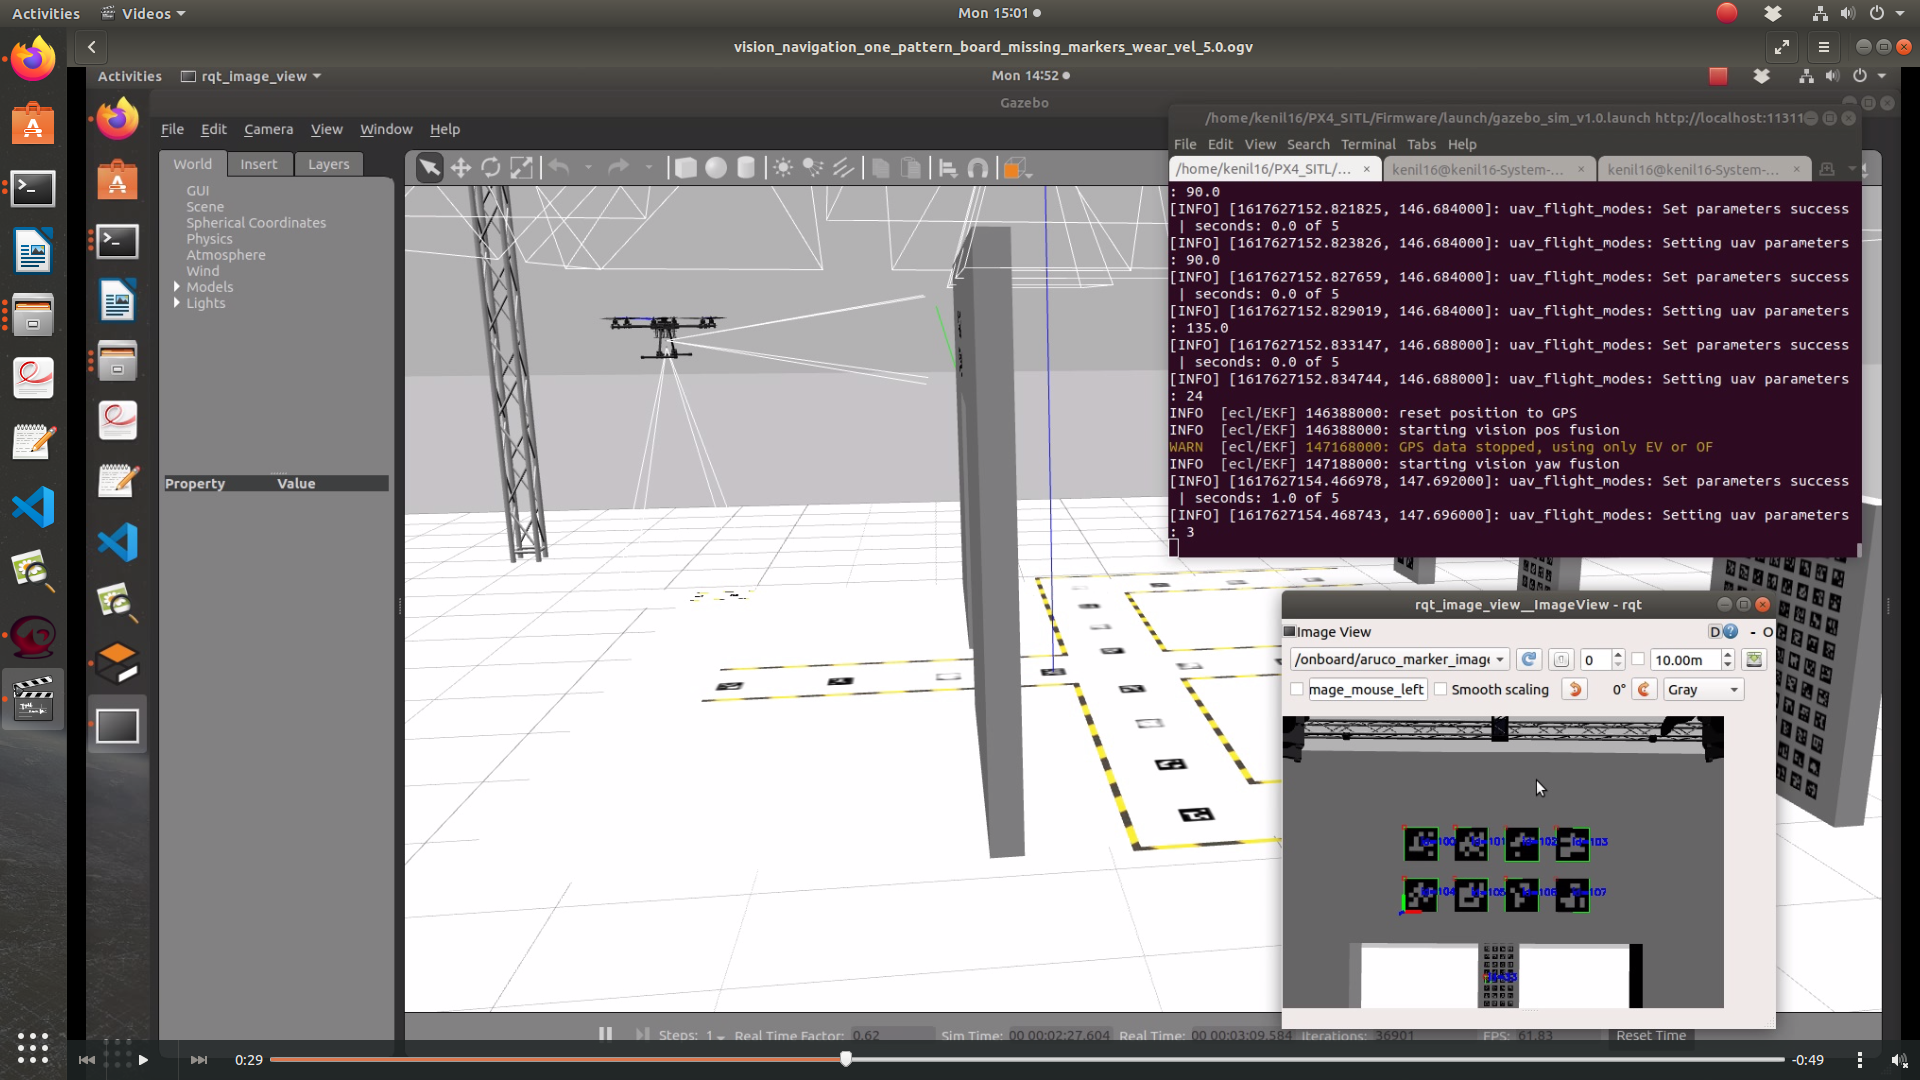
\includegraphics[width=\textwidth]{../Figures/vision_navigation/gps2vision.png}
        \caption{}
        \label{fig:vision_navigation_gps2vision}
    \end{subfigure}
     \hspace{0.2em}
    \begin{subfigure}[t]{.30\textwidth}
        \centering
        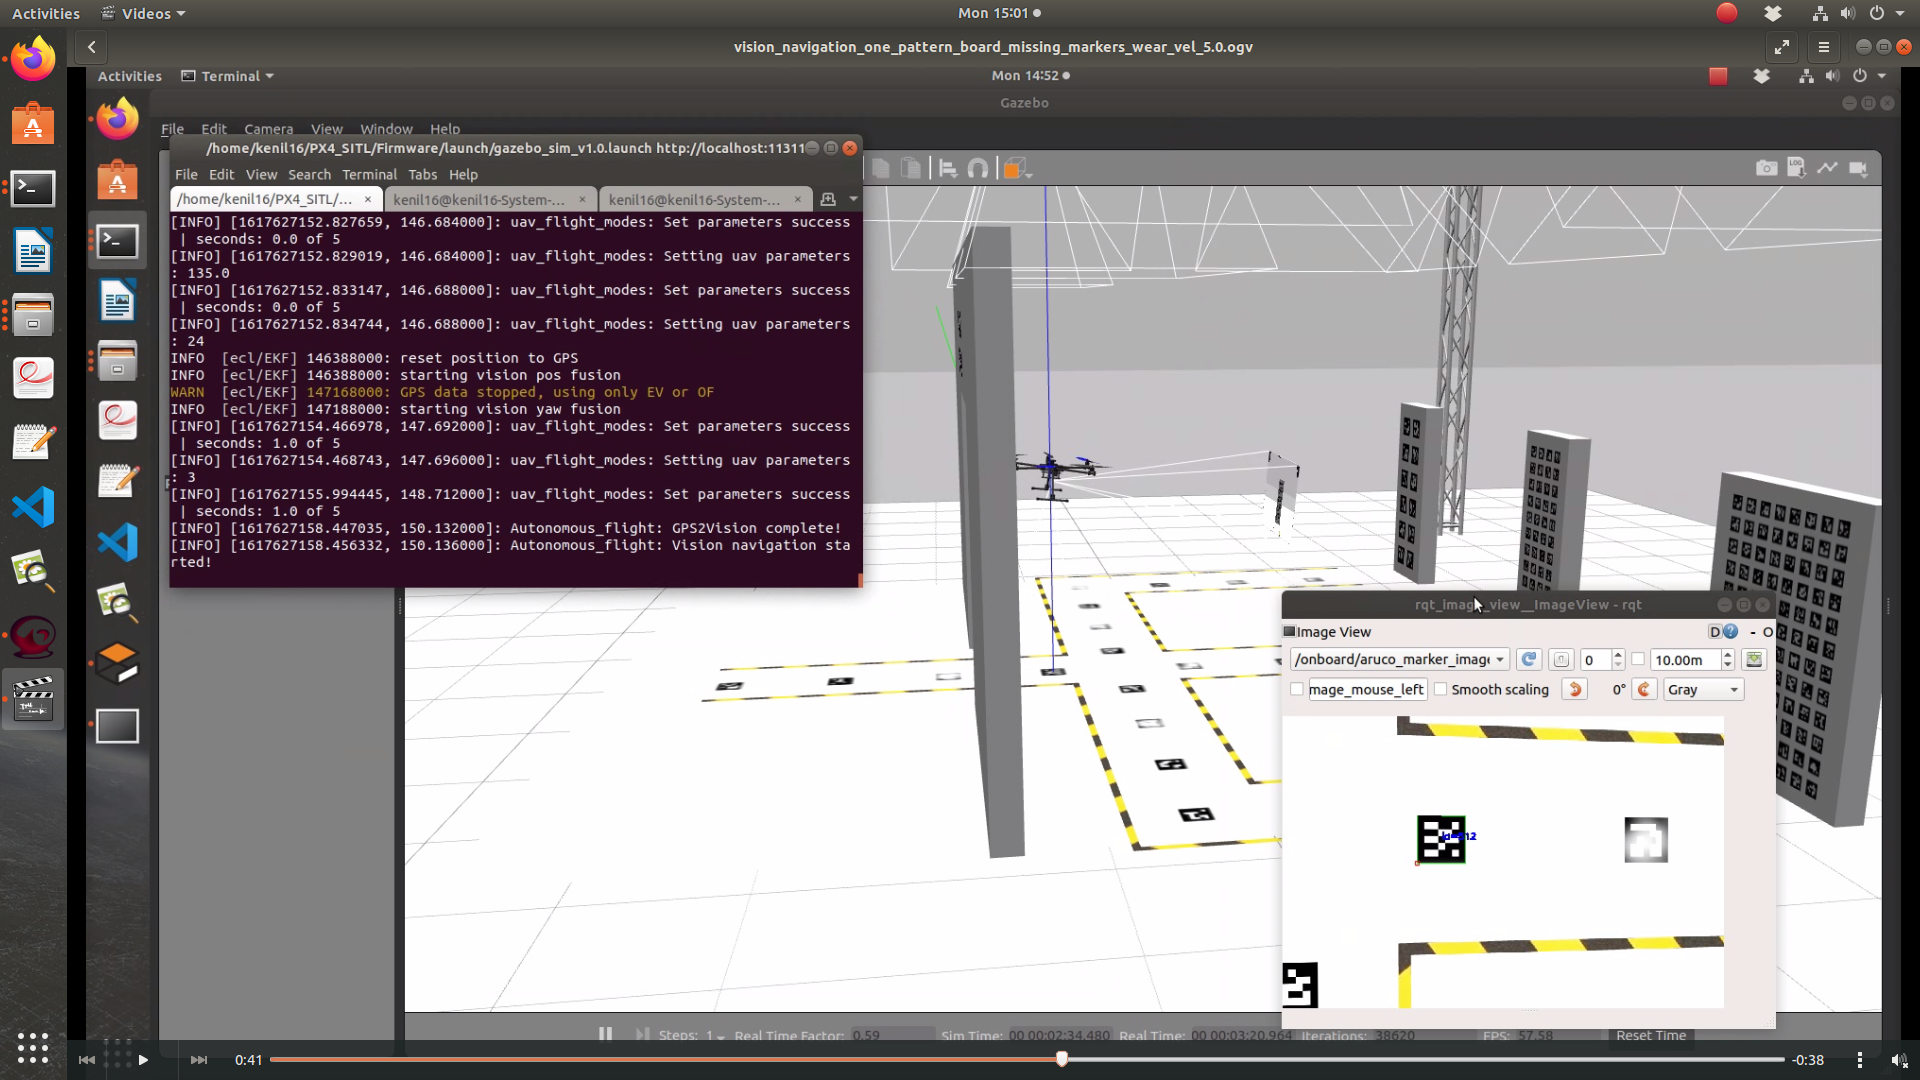
\includegraphics[width=\textwidth]{../Figures/vision_navigation/vision_navigation_one.png}
        \caption{}
        \label{fig:vision_navigation_vision_navigation_one}
    \end{subfigure}
     \hspace{0.2em}
    \begin{subfigure}[t]{.30\textwidth}
        \centering
        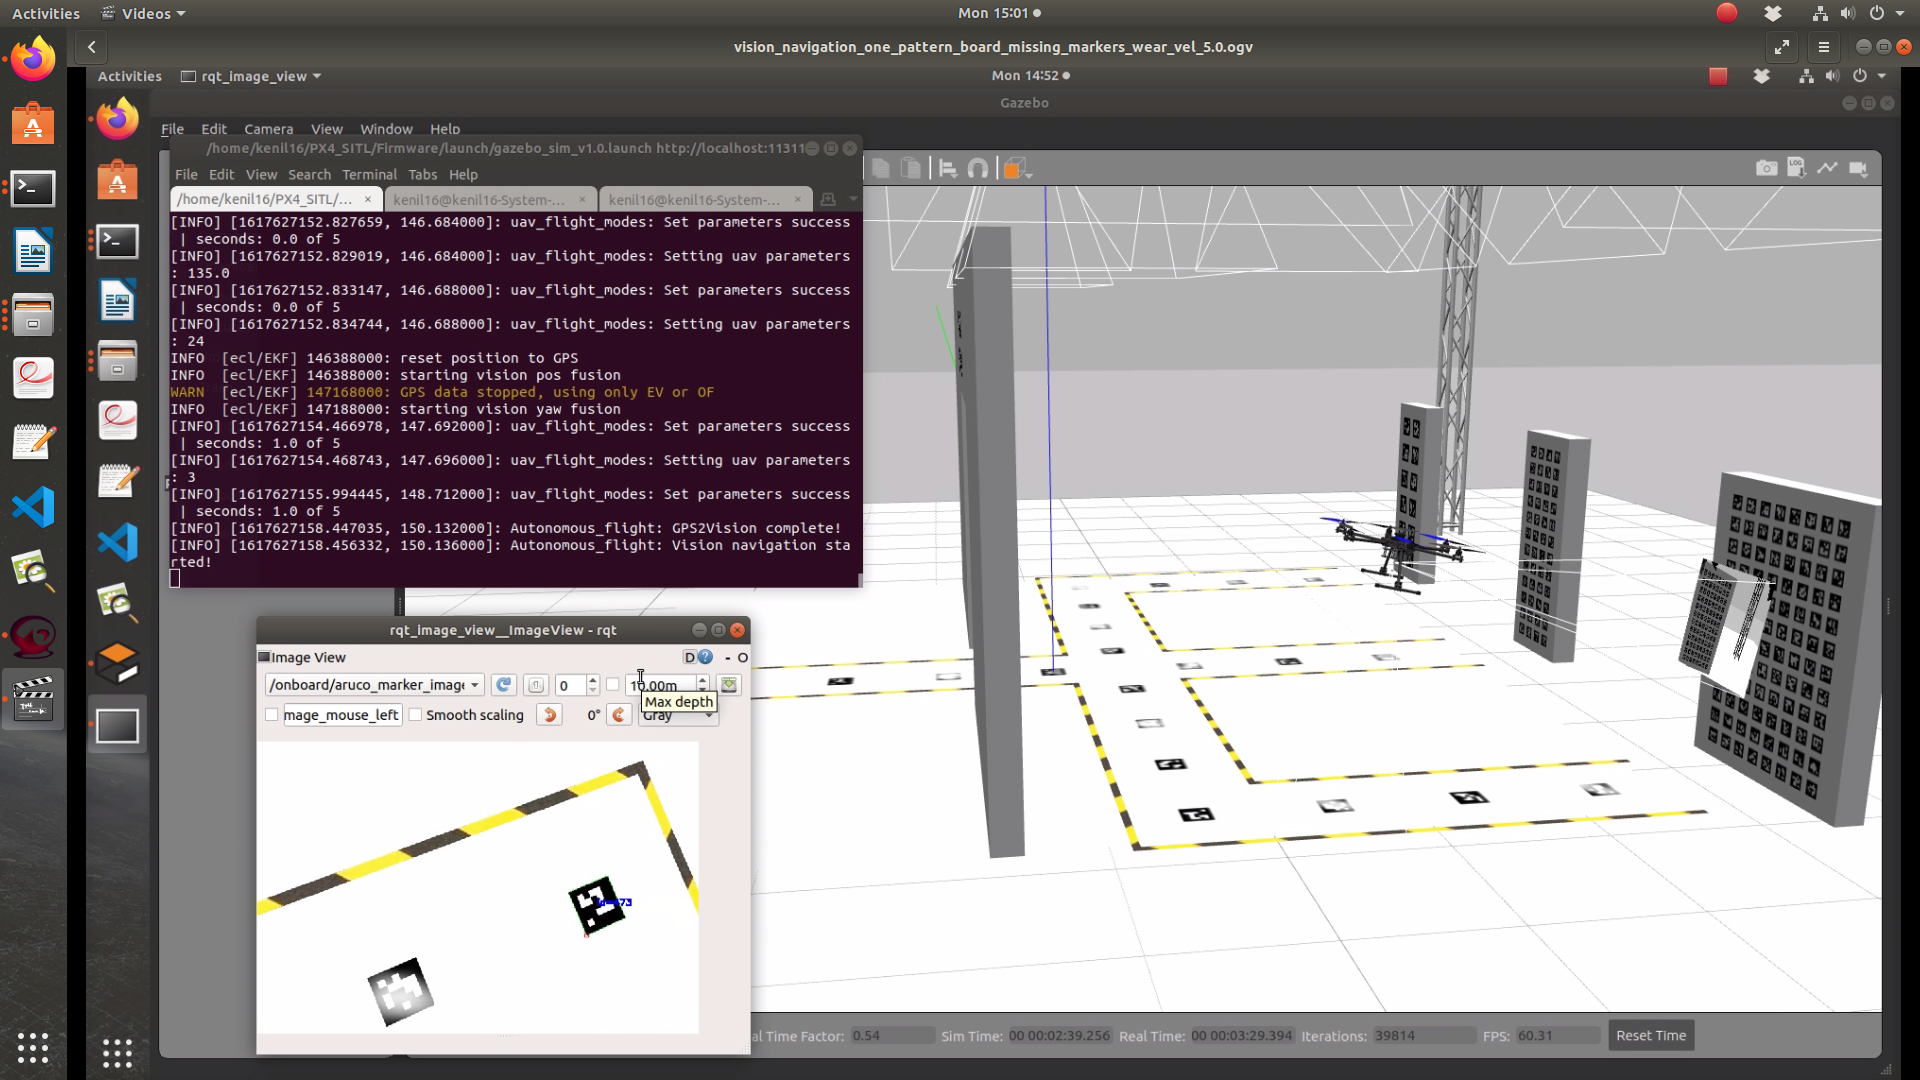
\includegraphics[width=\textwidth]{../Figures/vision_navigation/vision_navigation_two.png}
        \caption{}
        \label{fig:vision_navigation_vision_navigation_two}
    \end{subfigure}
    \caption{Illustrations of the vision based navigation test. The UAV initially starts in front of the GPS2Vision board as seen in Figure \ref{fig:vision_navigation_gps2vision}. Then it moves either to landing station one, two or three and then back to its initial position where the target landing station is chosen randomly at the initialization of the test. In this case, the UAV can be seen to move to landing station three in Figures \ref{fig:vision_navigation_vision_navigation_one} and \ref{fig:vision_navigation_vision_navigation_two}. Videos of the test can be seen on Github using \href{https://github.com/Kenil16/master_project/tree/master/test_videos/vision_navigation_full_marker_board_vel_1.0}{Vision navigation ( full ArUco board)} and \href{https://github.com/Kenil16/master_project/tree/master/test_videos/vision_navigation_one_pattern_board_missing_markers_wear_vel_5.0}{Vision navigation (ArUco board with missing markers)}}
    \label{fig:vision_navigation}
\end{figure}

\begin{figure}[H]
    \centering
    \begin{subfigure}[t]{.20\textwidth}
        \centering
        \includegraphics[width=\textwidth]{../Figures/vision_navigation/grid_board_new_200_full.png}
        \caption{}
        \label{fig:vision_navigation_full_pattern_board}
    \end{subfigure}
     \hspace{0.2em}
    \begin{subfigure}[t]{.20\textwidth}
        \centering
        \includegraphics[width=\textwidth]{../Figures/vision_navigation/grid_board_new_200_big_onepattern.png}
        \caption{}
        \label{fig:vision_navigation_one_pattern_board}
    \end{subfigure}
     \hspace{0.2em}
    \begin{subfigure}[t]{.20\textwidth}
        \centering
        \includegraphics[width=\textwidth]{../Figures/vision_navigation/grid_board_new_200_big_onepattern_missing_markers1.png}
        \caption{}
        \label{fig:vision_navigation_one_pattern_board_missing_markers}
    \end{subfigure}
         \hspace{0.2em}
    \begin{subfigure}[t]{.20\textwidth}
        \centering
        \includegraphics[width=\textwidth]{../Figures/vision_navigation/grid_board_new_200_big_onepattern_missing_markers_wear.png}
        \caption{}
        \label{fig:vision_navigation_one_pattern_board_missing_markers_wear}
    \end{subfigure}
    \caption{Illustrations of the ArUco boards used which are located on the ground. In Figure \ref{fig:vision_navigation_full_pattern_board}, a complete $25 \times 25$ ArUco board is used for test 1. A one pattern ArUco board is used in \ref{fig:vision_navigation_one_pattern_board} for test 2. The same one pattern ArUco board is used in \ref{fig:vision_navigation_one_pattern_board_missing_markers} for test 3 and \ref{fig:vision_navigation_one_pattern_board_missing_markers_wear} for test 4 and 5, but with a meter between the markers (missing markers) and with some of the markers blurred in Figure \ref{fig:vision_navigation_one_pattern_board_missing_markers_wear} to illustrate wear due to walking on the markers}  
    \label{fig:vision_navigation_boards}
\end{figure}

\begin{table}[H]
    \centering
    \addtolength{\leftskip} {-2cm}
    \addtolength{\rightskip}{-2cm}
        \caption{Statistics of the results in the vision navigation tests. The mean error can be seen to be in the range of centimeters in all tests, but with an increase when the number of visible markers decreases and speed increases. The large errors are primarily caused by a time delay between the ground truth of the UAV and the estimated pose based on sensor fusion}
        \pgfplotstabletypeset[normal,
                columns/eg/.style={
                column name={Runs},
                dec sep align
        }
        ]{ %
        Estimation error & eg & Waypoint error & Vel (Horizontal) & Mean position & STD position & Mean angle & STD angle\\
        \topmidheader{9}{\textbf{Test 1}}
        Sensor fusion & 20 & $0.1 m$ & $1\frac{m}{s}$ & $2.44cm$ & $2.51cm$ & $1.59 ^{\circ}$ & $9.68^{\circ}$\\
        \midheader{9}{\textbf{Test 2}}
        Sensor fusion & 20 & $0.1 m$ & $1\frac{m}{s}$ &$2.44cm$ & $2.29cm$ & $1.30 ^{\circ}$ & $7.44^{\circ}$\\
        \midheader{9}{\textbf{Test 3}}
        Sensor fusion & 20 & $0.1 m$ & $1\frac{m}{s}$ & $3.19cm$ & $3.28cm$ & $1.99 ^{\circ}$ & $10.88^{\circ}$\\
        \midheader{9}{\textbf{Test 4}}
        Sensor fusion & 20 & $0.1 m$ & $1\frac{m}{s}$ & $4.21cm$ & $3.96cm$ & $3.09 ^{\circ}$ & $11.99^{\circ}$\\
        \midheader{9}{\textbf{Test 5}}
        Sensor fusion & 20 & $0.1 m$ & $5\frac{m}{s}$ & $5.66cm$ & $5.79cm$ & $6.89 ^{\circ}$ & $22.29^{\circ}$\\}
        \label{tab:vision_navigation_stastitics}
\end{table}


\begin{figure}[H]
    \centering
    \begin{subfigure}[t]{.30\textwidth}
        \centering
        \includegraphics[width=\textwidth]{../Figures/vision_navigation/pose_error_x_test2.png}
        \caption{}
        \label{fig:vision_navigation_error_x}
    \end{subfigure}
     \hspace{0.2em}
    \begin{subfigure}[t]{.30\textwidth}
        \centering
        \includegraphics[width=\textwidth]{../Figures/vision_navigation/pose_error_y_test2.png}
        \caption{}
        \label{fig:vision_navigation_error_y}
    \end{subfigure}
     \hspace{0.2em}
    \begin{subfigure}[t]{.30\textwidth}
        \centering
        \includegraphics[width=\textwidth]{../Figures/vision_navigation/pose_error_z_test2.png}
        \caption{}
        \label{fig:vision_navigation_error_z}
    \end{subfigure}
    \caption{Illustration of the position estimation error using sensor fusion for test 1. It can be seen that the error increases a lot when large changes in the position occurs. This is because of a delay between the estimated position and the ground truth. This delay is even clearer in Figure \ref{fig:vision_navigation_error_yaw} when zooming in on the graph}
    \label{fig:vision_navigation_error_pos}
\end{figure}

\begin{figure}[H]
    \centering
    \begin{subfigure}[t]{.30\textwidth}
        \centering
        \includegraphics[width=\textwidth]{../Figures/vision_navigation/pose_error_roll_test2.png}
        \caption{}
        \label{fig:vision_navigation_error_roll}
    \end{subfigure}
     \hspace{0.2em}
    \begin{subfigure}[t]{.30\textwidth}
        \centering
        \includegraphics[width=\textwidth]{../Figures/vision_navigation/pose_error_pitch_test2.png}
        \caption{}
        \label{fig:vision_navigation_error_pitch}
    \end{subfigure}
     \hspace{0.2em}
    \begin{subfigure}[t]{.30\textwidth}
        \centering
        \includegraphics[width=\textwidth]{../Figures/vision_navigation/pose_error_yaw_test2.png}
        \caption{}
        \label{fig:vision_navigation_error_yaw}
    \end{subfigure}
    \caption{Illustration of the angle estimation error using sensor fusion for test 1. It can be seen that the error increases a lot when large changes in the angles occurs. This is because of a delay between the estimated angle and the ground truth. This delay leads to very large errors especially in yaw as seen in Figure \ref{fig:vision_navigation_error_yaw}}
    \label{fig:vision_navigation_error_angle}
\end{figure}

\begin{figure}[H]
    \centering
    \begin{subfigure}[t]{.30\textwidth}
        \centering
        \includegraphics[width=\textwidth]{../Figures/vision_navigation/test1_full_pattern_board/2d_path.png}
        \caption{}
        \label{fig:vision_navigation_2d_path_full_board}
    \end{subfigure}
     \hspace{0.2em}
    \begin{subfigure}[t]{.30\textwidth}
        \centering
        \includegraphics[width=\textwidth]{../Figures/vision_navigation/test4_one_pattern_missing_markers_wear_board/2d_path.png}
        \caption{}
        \label{fig:vision_navigation_2d_path_missing_markers_wear_vel_1.0}
    \end{subfigure}
     \hspace{0.2em}
    \begin{subfigure}[t]{.30\textwidth}
        \centering
        \includegraphics[width=\textwidth]{../Figures/vision_navigation/test5_one_pattern_missing_markers_wear_board/2d_path.png}
        \caption{}
        \label{fig:vision_navigation_2d_path_missing_markers_wear_vel_5.0}
    \end{subfigure}
    \caption{Illustrations of the ground truth path of the UAV seen from above in Figure \ref{fig:vision_navigation_2d_path_full_board}, \ref{fig:vision_navigation_2d_path_missing_markers_wear_vel_1.0} and \ref{fig:vision_navigation_2d_path_missing_markers_wear_vel_5.0} for test 1, 4 and 5 respectively. The blue dots illustrates the target setpoints when going to either landing station one, two or three. The gray lines defines the wanted trajectories and black lines the actual path of the UAV. Each test was performed for twenty runs}
    \label{fig:vision_navigation_2d_path}
\end{figure}  

In order to replicate the tests, the command in Listing \ref{lst:vision_navigation_test} can be run from the terminal.

\definecolor{lightgreen}{rgb}{0.56, 0.93, 0.56}
\definecolor{moonstoneblue}{rgb}{0.45, 0.66, 0.76}
\begin{listing}[H] 
\begin{tcolorbox}[
    enhanced,
    attach boxed title to top left={xshift=6mm,yshift=-3mm},
    colback=lightgreen!20,
    colframe=lightgreen,
    fonttitle=\bfseries\color{black},
]
\begin{minted}[ numbersep=6pt, linenos=true, breaklines=true, breakanywhere=true, mathescape, escapeinside=||,fontsize=\small]{bash}
#For execution of the giving test
roslaunch px4 gazebo_sim_v1.0.launch worlds:=optitrack_big_board_onepattern.world drone_control_args:="vision_navigation_test" x:=-3.0 y:=0.0 headless:=false gui:=true
\end{minted}
\end{tcolorbox}
\caption{Command to be used to replicate the test}
\label{lst:vision_navigation_test}    
\end{listing} 

Here the \textit{.world} file must be changed in Listing \ref{lst:vision_navigation_test} to optitrack\_big\_board\_full.world, optitrack\_big\_board\_onepattern.world and optitrack\_big\_board\_onepattern\_missing\_markers.world for the configuration in Figure \ref{fig:vision_navigation_full_pattern_board}, \ref{fig:vision_navigation_one_pattern_board}, \ref{fig:vision_navigation_one_pattern_board_missing_markers} and for the configuration with added custom wear optitrack\_big\_board\_onepattern\_missing\_markers\_wear.world  for  \ref{fig:vision_navigation_one_pattern_board_missing_markers_wear} respectively. 

\subsubsection{Vision based landing}
\label{sec:vision_based_landing}

\begin{figure}[H]
    \centering
    \begin{subfigure}[t]{.30\textwidth}
        \centering
        \includegraphics[width=\textwidth]{../Figures/landing_test/landing_station_one.png}
        \caption{}
        \label{fig:vision_based_landing_landing_station_one}
    \end{subfigure}
     \hspace{0.2em}
    \begin{subfigure}[t]{.30\textwidth}
        \centering
        \includegraphics[width=\textwidth]{../Figures/landing_test/landing_station_two.png}
        \caption{}
        \label{fig:vision_based_landing_landing_station_two}
    \end{subfigure}
     \hspace{0.2em}
    \begin{subfigure}[t]{.30\textwidth}
        \centering
        \includegraphics[width=\textwidth]{../Figures/landing_test/landing_station_three.png}
        \caption{}
        \label{fig:vision_based_landing_landing_station_three}
    \end{subfigure}
    \caption{Illustrations of the landing test. The UAV is set to move between the landing stations in a random order and make a landing using either landing station one, two or three which can be seen in Figures \ref{fig:vision_based_landing_landing_station_one}, \ref{fig:vision_based_landing_landing_station_two} and \ref{fig:vision_based_landing_landing_station_three} respectively. A video of the test can be seen on Github using \href{https://github.com/Kenil16/master_project/tree/master/test_videos/vision_landing_precision_and_accuracy_vertical_vel_0.5_max_error_0.05}{Vision based landing}}
    \label{fig:vision_based_landing_landing_stations}
\end{figure}  

\begin{table}[H]
    \centering
    \addtolength{\leftskip} {-2cm}
    \addtolength{\rightskip}{-2cm}
        \caption{Statistics of the results from landing tests. Each test runs for 100 landings randomly picked between landing stations. The error between the wanted landing setpoint and actual end position is defined with minimum, maximum, mean and STD error. The stabilize time is the time it takes the UAV to settle in front of the ArUco landing board before beginning the actual landing. The waypoint error defines the maximum allowed error, as already mentioned, before moving on to the next waypoint (landing is this case). It may be noticed that a decrease in stabilize and landing time comes with a cost of a larger final landing error. Also the velocity (vertical) has an impact on the final landing error}
        \pgfplotstabletypeset[normal,
                columns/eg/.style={
                column name={Runs},
                dec sep align
        }
        ]{ %
        Station & eg & Success & WP error & Vel & Min & Max & Mean & STD & Stabilize time & Landing time\\
        \topmidheader{12}{\textbf{Test 1}}
        One         & 35   & 32  & $0.1 m$ & $0.1 \frac{m}{s}$ & $1.60cm$ & $12.46cm$ & $5.81cm$ & $3.02cm$ & $3.60s$ &$11.51s$\\
        two         & 30  & 28   & $0.1 m$ & $0.1 \frac{m}{s}$ & $0.70cm$ & $11.83 cm$& $5.79cm$ & $2.54cm$& $0.70s$ &$11.76s$\\     
        Three       & 35  & 32   & $0.1 m$ & $0.1 \frac{m}{s}$ & $0.62cm$ & $10.75cm$ & $5.86cm$ & $2.50cm$& $3.22s$ &$11.82s$\\    
        \midheader{12}{\textbf{Test 2}}
        One         & 33   & 25   & $0.1 m$ & $0.5 \frac{m}{s}$ & $2.20cm$ & $15.04cm$ & $8.00cm$ & $2.67cm$ & $2.63s$ &$3.00s$\\
        two         & 29  & 25   & $0.1 m$ & $0.5 \frac{m}{s}$ & $3.18cm$ & $11.60 cm$& $7.62cm$ & $2.19cm$& $0.20s$ &$3.00s$\\     
        Three       & 38  & 27   & $0.1 m$ & $0.5 \frac{m}{s}$ & $1.11cm$ & $14.63cm$ & $7.87cm$ & $3.25cm$& $2.18s$ &$3.02s$\\    
        \midheader{12}{\textbf{Test 3}}
        One         & 32   & 19   & $0.1 m$ & $0.9 \frac{m}{s}$ & $4.63cm$ & $14.01cm$ & $9.25cm$ & $2.27cm$ & $1.68s$ &$2.15s$\\
        two         & 36  & 18  & $0.1 m$ & $0.9 \frac{m}{s}$ & $4.79cm$ & $14.00 cm$& $9.54cm$ & $1.92cm$& $0.19s$ &$2.13s$\\     
        Three       & 32   & 21  & $0.1 m$ & $0.9 \frac{m}{s}$ & $3.35cm$ & $18.45cm$ & $9.45cm$ & $2.88cm$& $2.09s$ &$2.18s$\\}
        \label{tab:vision_based_landing_statistics_waypoint_error_0.1}
\end{table}

\begin{figure}[H]
    \centering
    \begin{subfigure}[t]{.30\textwidth}
        \centering
        \includegraphics[width=\textwidth]{../Figures/landing_test/test3_speed_0.9_error_0.1/landing_for_station_one.png}
        \caption{}
        \label{fig:vision_based_landing_landing_station_one_test3}
    \end{subfigure}
     \hspace{0.2em}
    \begin{subfigure}[t]{.30\textwidth}
        \centering
        \includegraphics[width=\textwidth]{../Figures/landing_test/test3_speed_0.9_error_0.1/landing_for_station_two.png}
        \caption{}
        \label{fig:vision_based_landing_landing_station_two_test3}
    \end{subfigure}
     \hspace{0.2em}
    \begin{subfigure}[t]{.30\textwidth}
        \centering
        \includegraphics[width=\textwidth]{../Figures/landing_test/test3_speed_0.9_error_0.1/landing_for_station_three.png}
        \caption{}
        \label{fig:vision_based_landing_landing_station_three_test3}
    \end{subfigure}
    \caption{Illustrations of the final landings seen from above for test 3 in Figure \ref{fig:vision_based_landing_landing_station_one_test3}, \ref{fig:vision_based_landing_landing_station_two_test3} and \ref{fig:vision_based_landing_landing_station_three_test3} for landing station one, two and three respectively. It may be noticed the error is quite big where the wanted landing position should be in the center of the green circle which illustrates a threshold for acceptance for $\pm 10$ centimeters}
    \label{fig:vision_based_landing_test3}
\end{figure}

\begin{table}[H]
    \centering
    \addtolength{\leftskip} {-2cm}
    \addtolength{\rightskip}{-2cm}
        \caption{Statistics of the results from landing tests. It can be seen that if the waypoint check error is set lower, meaning the UAV has to settle even more before landing. The error in the final landing position decreases quite a lot. But again this comes with a cost of a longer stabilization time. In the best case as seen from test 4, the mean landing position error is decreased to be in the order of centimeters with a maximum error just above ten centimeters}
        \pgfplotstabletypeset[normal,
                columns/eg/.style={
                column name={Runs},
                dec sep align
        }
        ]{ %
        Station & eg & Success & WP error & Vel & Min & Max & Mean & STD & Stabilize time & Landing time\\
        \topmidheader{12}{\textbf{Test 4}}
One         & 33    & 33  & $0.05 m$ & $0.1 \frac{m}{s}$ & $0.08cm$ & $9.46cm$ & $4.81cm$ & $2.15cm$ & $9.93s$ &$11.45s$\\
        two         & 33   & 32  & $0.05 m$ & $0.1 \frac{m}{s}$ & $0.97cm$ & $11.18 cm$& $4.74cm$ & $2.56cm$& $6.96s$ &$11.69s$\\     
        Three       & 34    & 33  & $0.05 m$ & $0.1 \frac{m}{s}$ & $0.19cm$ & $11.84cm$ & $4.54cm$ & $2.41cm$& $9.11s$ &$11.58s$\\        		\midheader{12}{\textbf{Test 5}}
        One         & 32    & 32  & $0.05 m$ & $0.5 \frac{m}{s}$ & $1.63cm$ & $9.84cm$ & $5.25cm$ & $2.36cm$ & $8.43s$ &$3.00s$\\
        two         & 32   & 29  & $0.05 m$ & $0.5 \frac{m}{s}$ & $1.31cm$ & $13.07 cm$& $5.98cm$ & $2.90cm$& $6.34s$ &$3.00s$\\     
        Three       & 36    & 35  & $0.05 m$ & $0.5 \frac{m}{s}$ & $0.45cm$ & $12.22cm$ & $4.98cm$ & $2.88cm$& $9.33s$ &$3.00s$\\				\midheader{12}{\textbf{Test 6}}
        One         & 32    & 30  & $0.05 m$ & $0.9 \frac{m}{s}$ & $0.20cm$ & $11.89cm$ & $4.96cm$ & $2.77cm$ & $9.18s$ &$2.28s$\\
        two         & 35   & 32  & $0.05 m$ & $0.9 \frac{m}{s}$ & $0.65cm$ & $14.13 cm$& $5.90cm$ & $3.32cm$& $5.91s$ &$2.34s$\\     
        Three       & 33    & 31  & $0.05 m$ & $0.9 \frac{m}{s}$ & $1.06cm$ & $13.54cm$ & $5.35cm$ & $2.70cm$& $8.54s$ &$2.36s$\\}
        \label{tab:vision_based_landing_statistics_waypoint_error_0.05}
\end{table}

\begin{figure}[H]
    \centering
    \begin{subfigure}[t]{.30\textwidth}
        \centering
        \includegraphics[width=\textwidth]{../Figures/landing_test/test4_speed_0.1_error_0.05/landing_for_station_one.png}
        \caption{}
        \label{fig:vision_based_landing_landing_station_one_test4}
    \end{subfigure}
     \hspace{0.2em}
    \begin{subfigure}[t]{.30\textwidth}
        \centering
        \includegraphics[width=\textwidth]{../Figures/landing_test/test4_speed_0.1_error_0.05/landing_for_station_two.png}
        \caption{}
        \label{fig:vision_based_landing_landing_station_two_test4}
    \end{subfigure}
     \hspace{0.2em}
    \begin{subfigure}[t]{.30\textwidth}
        \centering
        \includegraphics[width=\textwidth]{../Figures/landing_test/test4_speed_0.1_error_0.05/landing_for_station_three.png}
        \caption{}
        \label{fig:vision_based_landing_landing_station_three_test4}
    \end{subfigure}
    \caption{Illustrations of the final landings seen from above for test 4 in Figure \ref{fig:vision_based_landing_landing_station_one_test4}, \ref{fig:vision_based_landing_landing_station_two_test4} and \ref{fig:vision_based_landing_landing_station_three_test4} for landing station one, two and three respectively. It can be seen that lowering the checkpoint error as well as decreasing the landing speed (vertical velocity), the accuracy and precision of the landings increases quite a lot}
    \label{fig:vision_based_landing_test4}
\end{figure}

To see how well the UAV is capable of performing landings when using the ArUco pose estimations, the UAV was set to start at landing station one. Then randomly move between landing stations and each time perform a landing where the landing position would be compared to the target landing position for error analysis. This can be seen in Figure \ref{fig:vision_based_landing_landing_stations}.  

In order to replicate the tests, the command in Listing \ref{lst:landing_test} can be run from the terminal.

\definecolor{lightgreen}{rgb}{0.56, 0.93, 0.56}
\definecolor{moonstoneblue}{rgb}{0.45, 0.66, 0.76}
\begin{listing}[H] 
\begin{tcolorbox}[
    enhanced,
    attach boxed title to top left={xshift=6mm,yshift=-3mm},
    colback=lightgreen!20,
    colframe=lightgreen,
    fonttitle=\bfseries\color{black},
]
\begin{minted}[ numbersep=6pt, linenos=true, breaklines=true, breakanywhere=true, mathescape, escapeinside=||,fontsize=\small]{bash}
#For execution of the giving test
roslaunch px4 gazebo_sim_v1.0.launch worlds:=optitrack_big_board_onepattern.world drone_control_args:="landing_test" x:=3.0 y:=3.3 headless:=false gui:=true
\end{minted}
\end{tcolorbox}
\caption{Command to be used to replicate the test}
\label{lst:landing_test}    
\end{listing} 

\subsection{OptiTrack}
\label{sec:optitrack}

\subsubsection{Steady state ArUco pose estimation}
\label{sec:steady_state_aruco_pose_estimation}

\begin{figure}[H]
    \centering
    \begin{subfigure}[t]{.25\textwidth}
        \centering
        \includegraphics[height=4.0cm]{../Figures/optitrack/steady_state_pose_estimation_one.png}
        \caption{}
        \label{fig:steady_state_aruco_pose_estimation_board_one}
    \end{subfigure}
    \begin{subfigure}[t]{.25\textwidth}
        \centering
        \includegraphics[height=4.0cm]{../Figures/optitrack/steady_state_pose_estimation_two.png}
        \caption{}
        \label{fig:steady_state_aruco_pose_estimation_board_two}
    \end{subfigure}
    \begin{subfigure}[t]{.25\textwidth}
        \centering
        \includegraphics[height=4.0cm]{../Figures/optitrack/steady_state_pose_estimation_three.png}
        \caption{}
        \label{fig:steady_state_aruco_pose_estimation_board_three}
    \end{subfigure}
    \caption{Illustration of steady state ArUco pose estimation test. Here the UAV can be seen in front of the landing marker board one, two and three in Figure \ref{fig:steady_state_aruco_pose_estimation_board_one}, \ref{fig:steady_state_aruco_pose_estimation_board_two} and \ref{fig:steady_state_aruco_pose_estimation_board_three} respectively} 
    \label{fig:steady_state_aruco_pose_estimation_boards}
\end{figure}

\begin{table}[H]
    \centering
    \addtolength{\leftskip} {-2cm}
    \addtolength{\rightskip}{-2cm}
        \caption{Statistics of the results of the steady state ArUco pose estimation test. Here it may be noticed that a mean error in the order of a couple of degrees is present. This is because of a misalignment of the ground truth from the OptiTrack system to that of the estimations from the ArUco marker boards. The reason for this is the legs attached to the UAV not being perfectly equal in height and the stand in which the ArUco markers boards is placed does tilt just a little which means it board not being totally perpendicular to the ground. These offsets can be seen in Figure \ref{fig:optitrack_steady_state_pose_estimation_error_ori_test_five}}
        \pgfplotstabletypeset[normal,
                columns/eg/.style={
                column name={Runs},
                dec sep align
        }
        ]{ %
        Estimation error & eg & Wind & Mean position & STD position & Mean angle & STD angle\\
        \topmidheader{8}{\textbf{Test 1}}
ArUco pose landing board one       & 5      & No & $0.60cm $ & $0.05cm$ & $2.0^{\circ}$ & $0.04^{\circ}$\\
		\midheader{8}{\textbf{Test 2}}
ArUco pose landing board two       & 5      & No & $0.21cm $ & $0.10cm$ & $1.89^{\circ}$ & $0.06^{\circ}$\\
		\midheader{8}{\textbf{Test 3}}
ArUco pose landing board three       & 5      & No & $0.13cm $ & $0.01cm$ &
$3.15^{\circ}$ & $0.02^{\circ}$\\
 }
 \label{tab:optitrack_hold_pose_using_estimated_aruco_pose}
\end{table}

\begin{figure}[H]
    \centering
    \begin{subfigure}[t]{.30\textwidth}
        \centering
        \includegraphics[width=\textwidth]{../Figures/optitrack/steady_aruco_pose_estimation/pose_error_x_test1.png}
        \caption{}
        \label{fig:optitrack_steady_state_pose_estimation_error_x_test_five}
    \end{subfigure}
     \hspace{0.2em}
    \begin{subfigure}[t]{.30\textwidth}
        \centering
        \includegraphics[width=\textwidth]{../Figures/optitrack/steady_aruco_pose_estimation/pose_error_y_test1.png}
        \caption{}
        \label{fig:optitrack_steady_state_pose_estimation_error_y_test_five}
    \end{subfigure}
     \hspace{0.2em}
    \begin{subfigure}[t]{.30\textwidth}
        \centering
        \includegraphics[width=\textwidth]{../Figures/optitrack/steady_aruco_pose_estimation/pose_error_z_test1.png}
        \caption{}
        \label{fig:optitrack_steady_state_pose_estimation_error_z_test_five}
    \end{subfigure}
    \caption{Illustration of the ArUco position estimation error using the configuration in Figure \ref{fig:steady_state_aruco_pose_estimation_board_three}. It may be noticed that the error is quite small and only negligible deviations in the pose estimations exist compared to the ground truth from the OptiTrack system} 
    \label{fig:optitrack_steady_state_pose_estimation_error_pos_test_five}
\end{figure}


\begin{figure}[H]
    \centering
    \begin{subfigure}[t]{.30\textwidth}
        \centering
        \includegraphics[width=\textwidth]{../Figures/optitrack/steady_aruco_pose_estimation/pose_error_roll_test1.png}
        \caption{}
        \label{fig:optitrack_steady_state_pose_estimation_error_roll_test_five}
    \end{subfigure}
     \hspace{0.2em}
    \begin{subfigure}[t]{.30\textwidth}
        \centering
        \includegraphics[width=\textwidth]{../Figures/optitrack/steady_aruco_pose_estimation/pose_error_pitch_test1.png}
        \caption{}
        \label{fig:optitrack_steady_state_pose_estimation_error_pitch_test_five}
    \end{subfigure}
     \hspace{0.2em}
    \begin{subfigure}[t]{.30\textwidth}
        \centering
        \includegraphics[width=\textwidth]{../Figures/optitrack/steady_aruco_pose_estimation/pose_error_yaw_test1.png}
        \caption{}
        \label{fig:optitrack_steady_state_pose_estimation_error_yaw_test_five}
    \end{subfigure}
    \caption{Illustration of the ArUco angle estimation error using the configuration in Figure \ref{fig:steady_state_aruco_pose_estimation_board_three}. It may be noticed that an offset exist which is more noticeable in roll and pitch in Figure \ref{fig:optitrack_steady_state_pose_estimation_error_roll_test_five} and \ref{fig:optitrack_steady_state_pose_estimation_error_pitch_test_five} due to a misalignment of the OptiTrack system and the estimated ArUco marker boards}
    \label{fig:optitrack_steady_state_pose_estimation_error_ori_test_five}
\end{figure}


\subsubsection{Hold pose using estimated ArUco pose}
\label{sec:hold_pose_using_estimated_aruco_pose}

\begin{figure}[H]
    \centering
    \begin{subfigure}[t]{.31\textwidth}
        \centering
        \includegraphics[height=3.5cm]{../Figures/optitrack/hold_pose_using_estimated_aruco_pose_one.png}
        \caption{}
        \label{fig:optitrack_hold_pose_board_one}
    \end{subfigure}
    \begin{subfigure}[t]{.31\textwidth}
        \centering
        \includegraphics[height=3.5cm]{../Figures/optitrack/hold_pose_using_estimated_aruco_pose_two.png}
        \caption{}
        \label{fig:optitrack_hold_pose_board_two}
    \end{subfigure}
    \begin{subfigure}[t]{.31\textwidth}
        \centering
        \includegraphics[height=3.5cm]{../Figures/optitrack/hold_pose_using_estimated_aruco_pose_three.png}
        \caption{}
        \label{fig:optitrack_hold_pose_board_three}
    \end{subfigure}
    \caption{Illustrations}
    \label{fig:optitrack_hold_pose_boards}
\end{figure}

\begin{table}[H]
    \centering
    \addtolength{\leftskip} {-2cm}
    \addtolength{\rightskip}{-2cm}
        \caption{Statistics of the results of holding the pose using the ArUco landing boards. It may be noticed that as more ArUco markers are present in the image, the lesser is the pose estimation error. However, no significant decrease in the pose estimation error is seen between using landing board one and three even though the entire image is filled with ArUco markers as seen in Figure \ref{fig:hold_pose_aruco_board_five}}
        \pgfplotstabletypeset[normal,
                columns/eg/.style={
                column name={Runs},
                dec sep align
        }
        ]{ %
        Estimation error & eg & Wind & Mean position & STD position & Mean angle & STD angle\\
        \topmidheader{8}{\textbf{Test 1}}
ArUco pose landing board one       & 5      & No & $2.99cm $ & $0.35cm$ & $0.83^{\circ}$ & $0.18^{\circ}$\\
Setpoint         & 5      & No & $3.80cm$ & $3.19cm$ & $0.69^{\circ}$ & $0.27^{\circ}$\\
		\midheader{8}{\textbf{Test 2}}
ArUco pose landing board two       & 5      & No & $2.56cm $ & $0.31cm$ & $0.97^{\circ}$ & $0.17^{\circ}$\\
Setpoint         & 5      & No & $5.36cm$ & $3.13cm$ & $0.28^{\circ}$ & $0.21^{\circ}$\\
		\midheader{8}{\textbf{Test 3}}
ArUco pose landing board three       & 5      & No & $2.97cm $ & $0.23cm$ &
$1.17^{\circ}$ & $0.22^{\circ}$\\
Setpoint         & 5      & No & $4.54cm$ & $3.03cm$ & $0.87^{\circ}$ & $0.22^{\circ}$\\
 }
 \label{tab:optitrack_hold_pose_using_estimated_aruco_pose}
\end{table}


\begin{figure}[H]
    \centering
    \begin{subfigure}[t]{.30\textwidth}
        \centering
        \includegraphics[width=\textwidth]{../Figures/optitrack/hold_pose_using_estimated_aruco_pose/pose_error_x_test5.png}
        \caption{}
        \label{fig:optitrack_hold_pose_using_estimated_aruco_pose_error_x_test_five}
    \end{subfigure}
     \hspace{0.2em}
    \begin{subfigure}[t]{.30\textwidth}
        \centering
        \includegraphics[width=\textwidth]{../Figures/optitrack/hold_pose_using_estimated_aruco_pose/pose_error_y_test5.png}
        \caption{}
        \label{fig:optitrack_hold_pose_using_estimated_aruco_pose_error_y_test_five}
    \end{subfigure}
     \hspace{0.2em}
    \begin{subfigure}[t]{.30\textwidth}
        \centering
        \includegraphics[width=\textwidth]{../Figures/optitrack/hold_pose_using_estimated_aruco_pose/pose_error_z_test5.png}
        \caption{}
        \label{fig:optitrack_hold_pose_using_estimated_aruco_pose_error_z_test_five}
    \end{subfigure}
    \caption{Illustration of the pose estimation and setpoint error using configuration in Figure \ref{fig:hold_pose_aruco_board_one_5-7ms_wind}. It may be noticed that the pose estimation errors in x and y are in the orders of centimeters with a bit increase in error in z}
    \label{fig:optitrack_hold_pose_using_estimated_aruco_pose_error_pos_test_five}
\end{figure}


\begin{figure}[H]
    \centering
    \begin{subfigure}[t]{.30\textwidth}
        \centering
        \includegraphics[width=\textwidth]{../Figures/optitrack/hold_pose_using_estimated_aruco_pose/pose_error_roll_test5.png}
        \caption{}
        \label{fig:optitrack_hold_pose_using_estimated_aruco_pose_error_roll_test_five}
    \end{subfigure}
     \hspace{0.2em}
    \begin{subfigure}[t]{.30\textwidth}
        \centering
        \includegraphics[width=\textwidth]{../Figures/optitrack/hold_pose_using_estimated_aruco_pose/pose_error_pitch_test5.png}
        \caption{}
        \label{fig:optitrack_hold_pose_using_estimated_aruco_pose_error_pitch_test_five}
    \end{subfigure}
     \hspace{0.2em}
    \begin{subfigure}[t]{.30\textwidth}
        \centering
        \includegraphics[width=\textwidth]{../Figures/optitrack/hold_pose_using_estimated_aruco_pose/pose_error_yaw_test5.png}
        \caption{}
        \label{fig:optitrack_hold_pose_using_estimated_aruco_pose_error_yaw_test_five}
    \end{subfigure}
    \caption{Illustration of the pose estimation and setpoint error using configuration in Figure \ref{fig:hold_pose_aruco_board_one_5-7ms_wind}. It may be noticed that the pose estimation errors in x and y are in the orders of centimeters with a bit increase in error in z}
    \label{fig:optitrack_hold_pose_using_estimated_aruco_pose_error_ori_test_five}
\end{figure}


\end{document}